% svn info. These are modified by svn at checkout time.
% The last version of these macros found before the maketitle will be the one on the front page,
% so only the main file is tracked.
% Do not edit by hand!
\RCS$Revision: 37671 $
\RCS$HeadURL: svn+ssh://svn.cern.ch/reps/tdr2/papers/EWK-10-005/tags/1.0/EWK-10-005.tex $
\RCS$Id: EWK-10-005.tex 37671 2011-02-08 09:31:51Z gdaskal $
%%%%%%%%%%%%% ptdr definitions %%%%%%%%%%%%%%%%%%%%%
\def\Fileversion$#1: #2 ${\gdef\fileversion{#2}}
\def\Filedate$#1: #2-#3-#4 #5 ${\gdef\filedate{#2/#3/#4}}
\Fileversion$Revision: 227897 $
\Filedate$Date: 2014-02-16 08:24:34 -0600 (Sun, 16 Feb 2014) $
%%%%%%%%%%%%%%%%%%%%%%%%%%%%%%%%%%%%%%%%%%%%%%%%%%%%%%%%%%%%%%%%%%%%
%
%  CMS Common definitions style file
%
%  N.B. use of \newcommand rather than \newcommand means
%       that a definition is ignored if already specified
%
%                                              L. Taylor 18 Feb 2005
%%%%%%%%%%%%%%%%%%%%%%%%%%%%%%%%%%%%%%%%%%%%%%%%%%%%%%%%%%%%%%%%%%%%
\NeedsTeXFormat{LaTeX2e}
\ProvidesPackage{ptdr-definitions}[\filedate\space CMS Additional Macro Definitions (\fileversion)]
\RequirePackage{xspace}
\RequirePackage{amsmath}

% Some shorthand
% turn off italics
\newcommand {\etal}{\mbox{et al.}\xspace} %et al. - no preceding comma
\newcommand {\ie}{\mbox{i.e.}\xspace}     %i.e.
\newcommand {\eg}{\mbox{e.g.}\xspace}     %e.g.
\newcommand {\etc}{\mbox{etc.}\xspace}     %etc.
\newcommand {\vs}{\mbox{\sl vs.}\xspace}      %vs.
\newcommand {\mdash}{\ensuremath{\mathrm{-}}} % for use within formulas

% some terms whose definition we may change
\newcommand {\Lone}{Level-1\xspace} % Level-1 or L1 ?
\newcommand {\Ltwo}{Level-2\xspace}
\newcommand {\Lthree}{Level-3\xspace}

% Some software programs (alphabetized)
\newcommand{\ACERMC} {\textsc{AcerMC}\xspace}
\newcommand{\ALPGEN} {{\textsc{alpgen}}\xspace}
\newcommand{\CALCHEP} {{\textsc{CalcHEP}}\xspace}
\newcommand{\CHARYBDIS} {{\textsc{charybdis}}\xspace}
\newcommand{\CMKIN} {\textsc{cmkin}\xspace}
\newcommand{\CMSIM} {{\textsc{cmsim}}\xspace}
\newcommand{\CMSSW} {{\textsc{cmssw}}\xspace}
\newcommand{\COBRA} {{\textsc{cobra}}\xspace}
\newcommand{\COCOA} {{\textsc{cocoa}}\xspace}
\newcommand{\COMPHEP} {\textsc{CompHEP}\xspace}
\newcommand{\EVTGEN} {{\textsc{evtgen}}\xspace}
\newcommand{\FAMOS} {{\textsc{famos}}\xspace}
\newcommand{\GARCON} {\textsc{garcon}\xspace}
\newcommand{\GARFIELD} {{\textsc{garfield}}\xspace}
\newcommand{\GEANE} {{\textsc{geane}}\xspace}
\newcommand{\GEANTfour} {{\textsc{Geant4}}\xspace}
\newcommand{\GEANTthree} {{\textsc{geant3}}\xspace}
\newcommand{\GEANT} {{\textsc{geant}}\xspace}
\newcommand{\HDECAY} {\textsc{hdecay}\xspace}
\newcommand{\HERWIG} {{\textsc{herwig}}\xspace}
\newcommand{\HERWIGpp} {{\textsc{herwig++}}\xspace}
\newcommand{\POWHEG} {{\textsc{powheg}}\xspace}
\newcommand{\HIGLU} {{\textsc{higlu}}\xspace}
\newcommand{\HIJING} {{\textsc{hijing}}\xspace}
\newcommand{\IGUANA} {\textsc{iguana}\xspace}
\newcommand{\ISAJET} {{\textsc{isajet}}\xspace}
\newcommand{\ISAPYTHIA} {{\textsc{isapythia}}\xspace}
\newcommand{\ISASUGRA} {{\textsc{isasugra}}\xspace}
\newcommand{\ISASUSY} {{\textsc{isasusy}}\xspace}
\newcommand{\ISAWIG} {{\textsc{isawig}}\xspace}
\newcommand{\MADGRAPH} {\textsc{MadGraph}\xspace}
\newcommand{\MCATNLO} {\textsc{mc@nlo}\xspace}
\newcommand{\MCFM} {\textsc{mcfm}\xspace}
\newcommand{\MILLEPEDE} {{\textsc{millepede}}\xspace}
\newcommand{\ORCA} {{\textsc{orca}}\xspace}
\newcommand{\OSCAR} {{\textsc{oscar}}\xspace}
\newcommand{\PHOTOS} {\textsc{photos}\xspace}
\newcommand{\PROSPINO} {\textsc{prospino}\xspace}
\newcommand{\PYTHIA} {{\textsc{pythia}}\xspace}
\newcommand{\SHERPA} {{\textsc{sherpa}}\xspace}
\newcommand{\TAUOLA} {\textsc{tauola}\xspace}
\newcommand{\TOPREX} {\textsc{TopReX}\xspace}
\newcommand{\XDAQ} {{\textsc{xdaq}}\xspace}


%  Experiments
\newcommand {\DZERO}{D0\xspace}     %etc.


% Measurements and units...

\newcommand{\de}{\ensuremath{^\circ}}
\newcommand{\ten}[1]{\ensuremath{\times \text{10}^\text{#1}}}
\newcommand{\unit}[1]{\ensuremath{\text{\,#1}}\xspace}
\newcommand{\mum}{\ensuremath{\,\mu\text{m}}\xspace}
\newcommand{\micron}{\ensuremath{\,\mu\text{m}}\xspace}
\newcommand{\cm}{\ensuremath{\,\text{cm}}\xspace}
\newcommand{\mm}{\ensuremath{\,\text{mm}}\xspace}
\newcommand{\mus}{\ensuremath{\,\mu\text{s}}\xspace}
\newcommand{\keV}{\ensuremath{\,\text{ke\hspace{-.08em}V}}\xspace}
\newcommand{\MeV}{\ensuremath{\,\text{Me\hspace{-.08em}V}}\xspace}
\newcommand{\MeVns}{\ensuremath{\text{Me\hspace{-.08em}V}}\xspace} % no leading thinspace
\newcommand{\GeV}{\ensuremath{\,\text{Ge\hspace{-.08em}V}}\xspace}
\newcommand{\GeVns}{\ensuremath{\text{Ge\hspace{-.08em}V}}\xspace} % no leading thinspace
\newcommand{\gev}{\GeV}
\newcommand{\TeV}{\ensuremath{\,\text{Te\hspace{-.08em}V}}\xspace}
\newcommand{\TeVns}{\ensuremath{\text{Te\hspace{-.08em}V}}\xspace} % no leading thinspace
\newcommand{\PeV}{\ensuremath{\,\text{Pe\hspace{-.08em}V}}\xspace}
\newcommand{\keVc}{\ensuremath{{\,\text{ke\hspace{-.08em}V\hspace{-0.16em}/\hspace{-0.08em}}c}}\xspace}
\newcommand{\MeVc}{\ensuremath{{\,\text{Me\hspace{-.08em}V\hspace{-0.16em}/\hspace{-0.08em}}c}}\xspace}
\newcommand{\GeVc}{\ensuremath{{\,\text{Ge\hspace{-.08em}V\hspace{-0.16em}/\hspace{-0.08em}}c}}\xspace}
\newcommand{\GeVcns}{\ensuremath{{\text{Ge\hspace{-.08em}V\hspace{-0.16em}/\hspace{-0.08em}}c}}\xspace} % no leading thinspace
\newcommand{\TeVc}{\ensuremath{{\,\text{Te\hspace{-.08em}V\hspace{-0.16em}/\hspace{-0.08em}}c}}\xspace}
\newcommand{\keVcc}{\ensuremath{{\,\text{ke\hspace{-.08em}V\hspace{-0.16em}/\hspace{-0.08em}}c^\text{2}}}\xspace}
\newcommand{\MeVcc}{\ensuremath{{\,\text{Me\hspace{-.08em}V\hspace{-0.16em}/\hspace{-0.08em}}c^\text{2}}}\xspace}
\newcommand{\GeVcc}{\ensuremath{{\,\text{Ge\hspace{-.08em}V\hspace{-0.16em}/\hspace{-0.08em}}c^\text{2}}}\xspace}
\newcommand{\GeVccns}{\ensuremath{{\text{Ge\hspace{-.08em}V\hspace{-0.16em}/\hspace{-0.08em}}c^\text{2}}}\xspace} % no leading thinspace
\newcommand{\TeVcc}{\ensuremath{{\,\text{Te\hspace{-.08em}V\hspace{-0.16em}/\hspace{-0.08em}}c^\text{2}}}\xspace}

\newcommand{\pbinv} {\mbox{\ensuremath{\,\text{pb}^\text{$-$1}}}\xspace}
\newcommand{\fbinv} {\mbox{\ensuremath{\,\text{fb}^\text{$-$1}}}\xspace}
\newcommand{\nbinv} {\mbox{\ensuremath{\,\text{nb}^\text{$-$1}}}\xspace}
\newcommand{\mubinv} {\ensuremath{\,\mu\mathrm{b}^{-1}}\xspace}
\newcommand{\percms}{\ensuremath{\,\text{cm}^\text{$-$2}\,\text{s}^\text{$-$1}}\xspace}
\newcommand{\lumi}{\ensuremath{\mathcal{L}}\xspace}
\newcommand{\Lumi}{\ensuremath{\mathcal{L}}\xspace}%both upper and lower
%
% Need a convention here:
\newcommand{\LvLow}  {\ensuremath{\mathcal{L}=\text{10}^\text{32}\,\text{cm}^\text{$-$2}\,\text{s}^\text{$-$1}}\xspace}
\newcommand{\LLow}   {\ensuremath{\mathcal{L}=\text{10}^\text{33}\,\text{cm}^\text{$-$2}\,\text{s}^\text{$-$1}}\xspace}
\newcommand{\lowlumi}{\ensuremath{\mathcal{L}=\text{2}\times \text{10}^\text{33}\,\text{cm}^\text{$-$2}\,\text{s}^\text{$-$1}}\xspace}
\newcommand{\LMed}   {\ensuremath{\mathcal{L}=\text{2}\times \text{10}^\text{33}\,\text{cm}^\text{$-$2}\,\text{s}^\text{$-$1}}\xspace}
\newcommand{\LHigh}  {\ensuremath{\mathcal{L}=\text{10}^\text{34}\,\text{cm}^\text{$-$2}\,\text{s}^\text{$-$1}}\xspace}
\newcommand{\hilumi} {\ensuremath{\mathcal{L}=\text{10}^\text{34}\,\text{cm}^\text{$-$2}\,\text{s}^\text{$-$1}}\xspace}

% Physics symbols ...

\newcommand{\PT}{\ensuremath{p_{\mathrm{T}}}\xspace}
\newcommand{\pt}{\ensuremath{p_{\mathrm{T}}}\xspace}
\newcommand{\ET}{\ensuremath{E_{\mathrm{T}}}\xspace}
\newcommand{\HT}{\ensuremath{H_{\mathrm{T}}}\xspace}
\newcommand{\et}{\ensuremath{E_{\mathrm{T}}}\xspace}
\newcommand{\Em}{\ensuremath{E\hspace{-0.6em}/}\xspace}
\newcommand{\Pm}{\ensuremath{p\hspace{-0.5em}/}\xspace}
\newcommand{\PTm}{\ensuremath{{p}_\mathrm{T}\hspace{-1.02em}/\kern 0.5em}\xspace}
\newcommand{\PTslash}{\PTm}
\newcommand{\ETm}{\ensuremath{E_{\mathrm{T}}^{\text{miss}}}\xspace}
\newcommand{\MET}{\ETm}
\newcommand{\ETmiss}{\ETm}
\newcommand{\ETslash}{\ensuremath{E_{\mathrm{T}}\hspace{-1.1em}/\kern0.45em}\xspace}
\newcommand{\VEtmiss}{\ensuremath{{\vec E}_{\mathrm{T}}^{\text{miss}}}\xspace}
\newcommand{\ptvec}{\ensuremath{{\vec p}_{\mathrm{T}}}\xspace}

% roman face derivative
\newcommand{\dd}[2]{\ensuremath{\frac{\cmsSymbolFace{d} #1}{\cmsSymbolFace{d} #2}}}
\newcommand{\ddinline}[2]{\ensuremath{\cmsSymbolFace{d} #1/\cmsSymbolFace{d} #2}}
\newcommand{\rd}{\ensuremath{\cmsSymbolFace{d}}}
\newcommand{\re}{\ensuremath{\cmsSymbolFace{e}}}
% absolute value
\newcommand{\abs}[1]{\ensuremath{\lvert #1 \rvert}}



\ifthenelse{\boolean{cms@italic}}{\newcommand{\cmsSymbolFace}{\relax}}{\newcommand{\cmsSymbolFace}{\mathrm}}

% Particle names which track the italic/non-italic face convention
\newcommand{\zp}{\ensuremath{\cmsSymbolFace{Z}^\prime}\xspace} % plain Z'
\newcommand{\JPsi}{\ensuremath{\cmsSymbolFace{J}\hspace{-.08em}/\hspace{-.14em}\psi}\xspace} % J/Psi (no mass)
\newcommand{\Z}{\ensuremath{\cmsSymbolFace{Z}}\xspace} % plain Z (no superscript 0)
\newcommand{\ttbar}{\ensuremath{\cmsSymbolFace{t}\overline{\cmsSymbolFace{t}}}\xspace} % t-tbar

% Extensions for missing names in PENNAMES % note no xspace, to match syntax in PENNAMES
\newcommand{\cPgn}{\ensuremath{\nu}} % generic neutrino
\providecommand{\Pgn}{\ensuremath{\nu}} % generic neutrino
\newcommand{\cPagn}{\ensuremath{\overline{\nu}}} % generic neutrino
\providecommand{\Pagn}{\ensuremath{\overline{\nu}}} % generic neutrino
\newcommand{\cPgg}{\ensuremath{\gamma}} % gamma
\newcommand{\cPJgy}{\ensuremath{\cmsSymbolFace{J}\hspace{-.08em}/\hspace{-.14em}\psi}} % J/Psi (no mass)
\newcommand{\cPZ}{\ensuremath{\cmsSymbolFace{Z}}} % plain Z (no superscript 0)
\newcommand{\cPZpr}{\ensuremath{\cmsSymbolFace{Z}^\prime}} % plain Z'
\newcommand{\cPqt}{\ensuremath{\cmsSymbolFace{t}}} % t for t quark
\newcommand{\cPqb}{\ensuremath{\cmsSymbolFace{b}}} % b for b quark
\newcommand{\cPqc}{\ensuremath{\cmsSymbolFace{c}}} % c for c quark
\newcommand{\cPqs}{\ensuremath{\cmsSymbolFace{s}}} % s for s quark
\newcommand{\cPqu}{\ensuremath{\cmsSymbolFace{u}}} % u for u quark
\newcommand{\cPqd}{\ensuremath{\cmsSymbolFace{d}}} % d for d quark
\newcommand{\cPq}{\ensuremath{\cmsSymbolFace{q}}} % generic quark
\newcommand{\cPg}{\ensuremath{\cmsSymbolFace{g}}} % generic gluon
\newcommand{\cPG}{\ensuremath{\cmsSymbolFace{G}}} % Graviton
\newcommand{\cPaqt}{\ensuremath{\overline{\cmsSymbolFace{t}}}} % t for t anti-quark
\newcommand{\cPaqb}{\ensuremath{\overline{\cmsSymbolFace{b}}}} % b for b anti-quark
\newcommand{\cPaqc}{\ensuremath{\overline{\cmsSymbolFace{c}}}} % c for c anti-quark
\newcommand{\cPaqs}{\ensuremath{\overline{\cmsSymbolFace{s}}}} % s for s anti-quark
\newcommand{\cPaqu}{\ensuremath{\overline{\cmsSymbolFace{u}}}} % u for u anti-quark
\newcommand{\cPaqd}{\ensuremath{\overline{\cmsSymbolFace{d}}}} % d for d anti-quark
\newcommand{\cPaq}{\ensuremath{\overline{\cmsSymbolFace{q}}}} % generic anti-quark
\newcommand{\cPKstz}{\ensuremath{\cmsSymbolFace{K}^{\ast0}}\xspace} %note has xspace
% future symbols from heppennames2
\providecommand{\PH}{\ensuremath{\cmsSymbolFace{H}}\xspace} % plain Higgs
\providecommand{\PJGy}{\ensuremath{\cmsSymbolFace{J}\hspace{-.08em}/\hspace{-.14em}\psi}\xspace} % J/Psi (no mass)
\providecommand{\PBzs}{\ensuremath{\cmsSymbolFace{B}^0_\cmsSymbolFace{s}}\xspace} % B^0_s
\providecommand{\Pg}{\ensuremath{\cmsSymbolFace{g}}\xspace} % generic gluon
\providecommand{\PSg}{\ensuremath{\widetilde{\cmsSymbolFace{g}}}\xspace} % gluino
\providecommand{\PSQ}{\ensuremath{\widetilde{\cmsSymbolFace{q}}}\xspace} % squark
\providecommand{\PXXG}{\ensuremath{\cmsSymbolFace{G}}\xspace} % graviton
\providecommand{\PXXSG}{\ensuremath{\widetilde{\PXXG}}\xspace} % gravitino
\providecommand{\PSGcp}{\ensuremath{\widetilde{\chi}^+}\xspace}
\providecommand{\PSGc}{\ensuremath{\widetilde{\chi}}\xspace} % neutralino
\providecommand{\PSGcz}{\ensuremath{\widetilde{\chi}^0}\xspace} % neutralino with superscript 0
\providecommand{\PSGczDo}{\ensuremath{\widetilde{\chi}^{0}_{1}}\xspace} % neutralino
\providecommand{\PSGczDt}{\ensuremath{\widetilde{\chi}^{0}_{2}}\xspace} % neutralino
\providecommand{\PSGcpm}{\ensuremath{\widetilde{\chi}^\pm}\xspace} % neutralino
\providecommand{\Pl}{\ensuremath{\cmsSymbolFace{l}}\xspace} % non-ell lepton
\providecommand{\PAl}{\ensuremath{\overline{\cmsSymbolFace{l}}}\xspace} % non-ell anti-lepton
\providecommand{\PGnl}{\ensuremath{\nu_\cmsSymbolFace{l}}\xspace} % lepton neutrino
\providecommand{\PAGnl}{\ensuremath{\overline{\nu}_\cmsSymbolFace{l}}\xspace} % anti-lepton neutrino
\providecommand{\PQtpr}{\ensuremath{\cmsSymbolFace{t}^{\prime}}\xspace} % t'
\providecommand{\PAQtpr}{\ensuremath{\bar{\cmsSymbolFace{t}}^\prime}\xspace} % t'-bar; needs to be converted to overline-requires rework a la heppennames
\providecommand{\PQbpr}{\ensuremath{\cmsSymbolFace{b}^{\prime}}\xspace} % b'
\providecommand{\PAQbpr}{\ensuremath{\bar{\cmsSymbolFace{b}}^\prime}\xspace} % b'-bar; needs same as anti-t'
\providecommand{\PGg}{\ensuremath{\gamma}\xspace} % gamma
\providecommand{\PKzS}{\ensuremath{\cmsSymbolFace{K}^0_\cmsSymbolFace{S}}\xspace} % K short
\providecommand{\PBs}{\ensuremath{\cmsSymbolFace{B}_\cmsSymbolFace{s}}\xspace} % B sub s
\providecommand{\PSQt}{\ensuremath{\widetilde{\cmsSymbolFace{t}}}\xspace} % stop
\providecommand{\PZpr}{\ensuremath{\cmsSymbolFace{Z}^\prime}\xspace} % plain Z'
\providecommand{\PWpr}{\ensuremath{\cmsSymbolFace{W}^\prime}\xspace} % plain W'
\providecommand{\PGn}{\ensuremath{\nu}\xspace} % generic neutrino
\providecommand{\PAGn}{\ensuremath{\overline{\nu}}\xspace} % generic neutrino


% for APS style tables
\ifthenelse{\boolean{cms@external}}{%
\newenvironment{scotch}[1]{\protect\centering\ruledtabular\tabular{#1}}{\endtabular\endruledtabular}
}{
\newenvironment{scotch}[1]{\protect\centering\tabular{#1}\hline\hline}{\hline\endtabular}
}

% SM (still to be classified)

\newcommand{\AFB}{\ensuremath{A_\text{FB}}\xspace}
\newcommand{\wangle}{\ensuremath{\sin^{2}\theta_{\text{eff}}^\text{lept}(M^2_{\Z})}\xspace}
\newcommand{\stat}{\ensuremath{\,\text{(stat.)}}\xspace}
\newcommand{\syst}{\ensuremath{\,\text{(syst.)}}\xspace}
\newcommand{\lum}{\ensuremath{\,\text{(lum.)}}\xspace}
\newcommand{\kt}{\ensuremath{k_{\mathrm{T}}}\xspace}

\newcommand{\BC}{\ensuremath{\cmsSymbolFace{B_{c}}}\xspace}
\newcommand{\bbarc}{\ensuremath{\cPqb\cPaqc}\xspace}
\newcommand{\bbbar}{\ensuremath{\cPqb\cPaqb}\xspace}
\newcommand{\ccbar}{\ensuremath{\cPqc\cPaqc}\xspace}
\newcommand{\bspsiphi}{\ensuremath{\cmsSymbolFace{B_s} \to \JPsi\, \phi}\xspace}
\newcommand{\EE}{\ensuremath{\Pep\Pem}\xspace}
\newcommand{\MM}{\ensuremath{\Pgmp\Pgmm}\xspace}
\newcommand{\TT}{\ensuremath{\Pgt^{+}\Pgt^{-}}\xspace}

%%%  E-gamma definitions
\newcommand{\HGG}{\ensuremath{\cmsSymbolFace{H}\to\gamma\gamma}}
\newcommand{\GAMJET}{\ensuremath{\gamma + \text{jet}}}
\newcommand{\PPTOJETS}{\ensuremath{\Pp\Pp\to\text{jets}}}
\newcommand{\PPTOGG}{\ensuremath{\Pp\Pp\to\gamma\gamma}}
\newcommand{\PPTOGAMJET}{\ensuremath{\Pp\Pp\to\gamma + \mathrm{jet}}}
\newcommand{\MH}{\ensuremath{M_{\PH}}}
\newcommand{\RNINE}{\ensuremath{R_\mathrm{9}}}
\newcommand{\DR}{\ensuremath{\Delta R}}





%%%%%%
% From Albert
%

\newcommand{\ga}{\ensuremath{\gtrsim}}
\newcommand{\la}{\ensuremath{\lesssim}}
%
\newcommand{\swsq}{\ensuremath{\sin^2\theta_\cmsSymbolFace{W}}\xspace}
\newcommand{\cwsq}{\ensuremath{\cos^2\theta_\cmsSymbolFace{W}}\xspace}
\newcommand{\tanb}{\ensuremath{\tan\beta}\xspace}
\newcommand{\tanbsq}{\ensuremath{\tan^{2}\beta}\xspace}
\newcommand{\sidb}{\ensuremath{\sin 2\beta}\xspace}
\newcommand{\alpS}{\ensuremath{\alpha_S}\xspace}
\newcommand{\alpt}{\ensuremath{\tilde{\alpha}}\xspace}

\newcommand{\QL}{\ensuremath{\cmsSymbolFace{Q}_\cmsSymbolFace{L}}\xspace}
\newcommand{\sQ}{\ensuremath{\widetilde{\cmsSymbolFace{Q}}}\xspace}
\newcommand{\sQL}{\ensuremath{\widetilde{\cmsSymbolFace{Q}}_\cmsSymbolFace{L}}\xspace}
\newcommand{\ULC}{\ensuremath{\cmsSymbolFace{U}_\cmsSymbolFace{L}^\cmsSymbolFace{C}}\xspace}
\newcommand{\sUC}{\ensuremath{\widetilde{\cmsSymbolFace{U}}^\cmsSymbolFace{C}}\xspace}
\newcommand{\sULC}{\ensuremath{\widetilde{\cmsSymbolFace{U}}_\cmsSymbolFace{L}^\cmsSymbolFace{C}}\xspace}
\newcommand{\DLC}{\ensuremath{\cmsSymbolFace{D}_\cmsSymbolFace{L}^\cmsSymbolFace{C}}\xspace}
\newcommand{\sDC}{\ensuremath{\widetilde{\cmsSymbolFace{D}}^\cmsSymbolFace{C}}\xspace}
\newcommand{\sDLC}{\ensuremath{\widetilde{\cmsSymbolFace{D}}_\cmsSymbolFace{L}^\cmsSymbolFace{C}}\xspace}
\newcommand{\LL}{\ensuremath{\cmsSymbolFace{L}_\cmsSymbolFace{L}}\xspace}
\newcommand{\sL}{\ensuremath{\widetilde{\cmsSymbolFace{L}}}\xspace}
\newcommand{\sLL}{\ensuremath{\widetilde{\cmsSymbolFace{L}}_\cmsSymbolFace{L}}\xspace}
\newcommand{\ELC}{\ensuremath{\cmsSymbolFace{E}_\cmsSymbolFace{L}^\cmsSymbolFace{C}}\xspace}
\newcommand{\sEC}{\ensuremath{\widetilde{\cmsSymbolFace{E}}^\cmsSymbolFace{C}}\xspace}
\newcommand{\sELC}{\ensuremath{\widetilde{\cmsSymbolFace{E}}_\cmsSymbolFace{L}^\cmsSymbolFace{C}}\xspace}
\newcommand{\sEL}{\ensuremath{\widetilde{\cmsSymbolFace{E}}_\cmsSymbolFace{L}}\xspace}
\newcommand{\sER}{\ensuremath{\widetilde{\cmsSymbolFace{E}}_\cmsSymbolFace{R}}\xspace}
\newcommand{\sFer}{\ensuremath{\widetilde{\cmsSymbolFace{f}}}\xspace}
\newcommand{\sQua}{\ensuremath{\widetilde{\cmsSymbolFace{q}}}\xspace}
\newcommand{\sUp}{\ensuremath{\widetilde{\cmsSymbolFace{u}}}\xspace}
\newcommand{\suL}{\ensuremath{\widetilde{\cmsSymbolFace{u}}_\cmsSymbolFace{L}}\xspace}
\newcommand{\suR}{\ensuremath{\widetilde{\cmsSymbolFace{u}}_\cmsSymbolFace{R}}\xspace}
\newcommand{\sDw}{\ensuremath{\widetilde{\cmsSymbolFace{d}}}\xspace}
\newcommand{\sdL}{\ensuremath{\widetilde{\cmsSymbolFace{d}}_\cmsSymbolFace{L}}\xspace}
\newcommand{\sdR}{\ensuremath{\widetilde{\cmsSymbolFace{d}}_\cmsSymbolFace{R}}\xspace}
\newcommand{\sTop}{\ensuremath{\widetilde{\cmsSymbolFace{t}}}\xspace}
\newcommand{\stL}{\ensuremath{\widetilde{\cmsSymbolFace{t}}_\cmsSymbolFace{L}}\xspace}
\newcommand{\stR}{\ensuremath{\widetilde{\cmsSymbolFace{t}}_\cmsSymbolFace{R}}\xspace}
\newcommand{\stone}{\ensuremath{\widetilde{\cmsSymbolFace{t}}_1}\xspace}
\newcommand{\sttwo}{\ensuremath{\widetilde{\cmsSymbolFace{t}}_2}\xspace}
\newcommand{\sBot}{\ensuremath{\widetilde{\cmsSymbolFace{b}}}\xspace}
\newcommand{\sbL}{\ensuremath{\widetilde{\cmsSymbolFace{b}}_\cmsSymbolFace{L}}\xspace}
\newcommand{\sbR}{\ensuremath{\widetilde{\cmsSymbolFace{b}}_\cmsSymbolFace{R}}\xspace}
\newcommand{\sbone}{\ensuremath{\widetilde{\cmsSymbolFace{b}}_1}\xspace}
\newcommand{\sbtwo}{\ensuremath{\widetilde{\cmsSymbolFace{b}}_2}\xspace}
\newcommand{\sLep}{\ensuremath{\widetilde{\cmsSymbolFace{l}}}\xspace}
\newcommand{\sLepC}{\ensuremath{\widetilde{\cmsSymbolFace{l}}^\cmsSymbolFace{C}}\xspace}
\newcommand{\sEl}{\ensuremath{\widetilde{\cmsSymbolFace{e}}}\xspace}
\newcommand{\sElC}{\ensuremath{\widetilde{\cmsSymbolFace{e}}^\cmsSymbolFace{C}}\xspace}
\newcommand{\seL}{\ensuremath{\widetilde{\cmsSymbolFace{e}}_\cmsSymbolFace{L}}\xspace}
\newcommand{\seR}{\ensuremath{\widetilde{\cmsSymbolFace{e}}_\cmsSymbolFace{R}}\xspace}
\newcommand{\snL}{\ensuremath{\widetilde{\nu}_L}\xspace}
\newcommand{\sMu}{\ensuremath{\widetilde{\mu}}\xspace}
\newcommand{\sNu}{\ensuremath{\widetilde{\nu}}\xspace}
\newcommand{\sTau}{\ensuremath{\widetilde{\tau}}\xspace}
\newcommand{\Glu}{\ensuremath{\cmsSymbolFace{g}}\xspace}
\newcommand{\sGlu}{\ensuremath{\widetilde{\cmsSymbolFace{g}}}\xspace}
\newcommand{\Wpm}{\ensuremath{\cmsSymbolFace{W}^{\pm}}\xspace}
\newcommand{\sWpm}{\ensuremath{\widetilde{\cmsSymbolFace{W}}^{\pm}}\xspace}
\newcommand{\Wz}{\ensuremath{\cmsSymbolFace{W}^{0}}\xspace}
\newcommand{\sWz}{\ensuremath{\widetilde{\cmsSymbolFace{W}}^{0}}\xspace}
\newcommand{\sWino}{\ensuremath{\widetilde{\cmsSymbolFace{W}}}\xspace}
\newcommand{\Bz}{\ensuremath{\cmsSymbolFace{B}^{0}}\xspace}
\newcommand{\sBz}{\ensuremath{\widetilde{\cmsSymbolFace{B}}^{0}}\xspace}
\newcommand{\sBino}{\ensuremath{\widetilde{\cmsSymbolFace{B}}}\xspace}
\newcommand{\Zz}{\ensuremath{\cmsSymbolFace{Z}^{0}}\xspace}
\newcommand{\sZino}{\ensuremath{\widetilde{\cmsSymbolFace{Z}}^{0}}\xspace}
\newcommand{\sGam}{\ensuremath{\widetilde{\gamma}}\xspace}
\newcommand{\chiz}{\ensuremath{\widetilde{\chi}^{0}}\xspace}
\newcommand{\chip}{\ensuremath{\widetilde{\chi}^{+}}\xspace}
\newcommand{\chim}{\ensuremath{\widetilde{\chi}^{-}}\xspace}
\newcommand{\chipm}{\ensuremath{\widetilde{\chi}^{\pm}}\xspace}
\newcommand{\Hone}{\ensuremath{\cmsSymbolFace{H}_\cmsSymbolFace{d}}\xspace}
\newcommand{\sHone}{\ensuremath{\widetilde{\cmsSymbolFace{H}}_\cmsSymbolFace{d}}\xspace}
\newcommand{\Htwo}{\ensuremath{\cmsSymbolFace{H}_\cmsSymbolFace{u}}\xspace}
\newcommand{\sHtwo}{\ensuremath{\widetilde{\cmsSymbolFace{H}}_\cmsSymbolFace{u}}\xspace}
\newcommand{\sHig}{\ensuremath{\widetilde{\cmsSymbolFace{H}}}\xspace}
\newcommand{\sHa}{\ensuremath{\widetilde{\cmsSymbolFace{H}}_\cmsSymbolFace{a}}\xspace}
\newcommand{\sHb}{\ensuremath{\widetilde{\cmsSymbolFace{H}}_\cmsSymbolFace{b}}\xspace}
\newcommand{\sHpm}{\ensuremath{\widetilde{\cmsSymbolFace{H}}^{\pm}}\xspace}
\newcommand{\hz}{\ensuremath{\cmsSymbolFace{h}^{0}}\xspace}
\newcommand{\Hz}{\ensuremath{\cmsSymbolFace{H}^{0}}\xspace}
\newcommand{\Az}{\ensuremath{\cmsSymbolFace{A}^{0}}\xspace}
\newcommand{\Hpm}{\ensuremath{\cmsSymbolFace{H}^{\pm}}\xspace}
\newcommand{\sGra}{\ensuremath{\widetilde{\cmsSymbolFace{G}}}\xspace}
%
\newcommand{\mtil}{\ensuremath{\widetilde{m}}\xspace}
%
\newcommand{\rpv}{\ensuremath{\rlap{\kern.2em/}R}\xspace}
\newcommand{\LLE}{\ensuremath{LL\bar{E}}\xspace}
\newcommand{\LQD}{\ensuremath{LQ\bar{D}}\xspace}
\newcommand{\UDD}{\ensuremath{\overline{UDD}}\xspace}
\newcommand{\Lam}{\ensuremath{\lambda}\xspace}
\newcommand{\Lamp}{\ensuremath{\lambda'}\xspace}
\newcommand{\Lampp}{\ensuremath{\lambda''}\xspace}
%
\newcommand{\spinbd}[2]{\ensuremath{\bar{#1}_{\dot{#2}}}\xspace}

\newcommand{\MD}{\ensuremath{{M_\mathrm{D}}}\xspace}% ED mass
\newcommand{\Mpl}{\ensuremath{{M_\mathrm{Pl}}}\xspace}% Planck mass
\newcommand{\Rinv} {\ensuremath{{R}^{-1}}\xspace}
\endinput

%%%%%%%%%%%%%%%  Additional definitions %%%%%%%%%%%%%%%%%%%%%%%%
\newcommand{\comment}[1]{}
\newcommand{\pb}{\ensuremath{\mathrm{pb}}}%
\newcommand{\pp}{\ensuremath{\mathrm{pp}}}%
\newcommand{\Wo}{\ensuremath{\mathrm{W}}}%
\newcommand{\Wp}{\ensuremath{\mathrm{W^+}}}%
\newcommand{\Wm}{\ensuremath{\mathrm{W^-}}}%
\newcommand{\Zo}{\ensuremath{\mathrm{Z}}}%
\newcommand{\rts}{\ensuremath{\sqrt{s}}}%
\newcommand{\ra}{\ensuremath{\rightarrow}}%
\newcommand{\MN}{\ensuremath{\mu\nu}}%
\renewcommand{\EE}{\ensuremath{\mathrm{e}^+\mathrm{e}^-}}%
\newcommand{\EN}{\ensuremath{\mathrm{e}\nu}}%
\newcommand{\LN}{\ensuremath{\ell\nu}}%
\newcommand{\MW}{\ensuremath{\mathrm{m}_\Wo}}%
\newcommand{\MZ}{\ensuremath{\mathrm{m}_\Zo}}%
\newcommand{\MT}{\ensuremath{\mathrm{M}_T}}%
\newcommand{\MLL}{\ensuremath{\mathrm{M}_{\ell\ell}}}%
\newcommand{\met}{\ensuremath{{E\!\!\!/}_{\mathrm{T}}}\xspace}
\renewcommand{\ttbar}{\ensuremath{\mathrm{t}\bar{\mathrm{t}}}}%
\newcommand{\Wmn}{\ensuremath{\Wo \ra \MN}}%
\newcommand{\Wpmn}{\ensuremath{\Wp \ra \mu^+\nu}}%
\newcommand{\Wmmn}{\ensuremath{\Wm \ra \mu^-\overline{\nu}}}%
\newcommand{\Zmm}{\ensuremath{\Zo \ra \MM}}%
\newcommand{\Wtn}{\ensuremath{\Wo \ra \tau\nu}}%
\newcommand{\Ztt}{\ensuremath{\Zo \ra \tau^+\tau^-}}%
\newcommand{\ppZmm}{\pp \ra \Zo(\gamma^*) + X \ra \MM + X}%
\newcommand{\ppWmn}{\pp \ra \Wo + X \ra \MN + X}%
\newcommand{\ppWpmn}{\pp \ra \Wp + X \ra \mu^+\nu + X}%
\newcommand{\ppWmmn}{\pp \ra \Wm + X \ra \mu^-\overline{\nu} + X}%
\newcommand{\Wen}{\ensuremath{\Wo \ra \EN}}%
\newcommand{\Wpen}{\ensuremath{\Wp \ra \mathrm{e}^+\nu}}%
\newcommand{\Wmen}{\ensuremath{\Wm \ra \mathrm{e}^-\overline{\nu}}}%
\newcommand{\Zee}{\ensuremath{\Zo \ra \EE}}%
\newcommand{\ppZee}{\pp \ra \Zo(\gamma^*) + X \ra \EE + X}%
\newcommand{\ppWen}{\pp \ra \Wo + X \ra \EN + X}%
\newcommand{\ppWpen}{\pp \ra \Wp + X \ra \mathrm{e}^+\nu  + X}%
\newcommand{\ppWmen}{\pp \ra \Wm + X \ra \mathrm{e}^-\overline{\nu} + X}%

\newcommand{\Wln}{\ensuremath{\Wo \ra \LN}}%
\newcommand{\Wpln}{\ensuremath{\Wp \ra \ell^+\nu}}%
\newcommand{\Wmln}{\ensuremath{\Wm \ra \ell^-\overline{\nu}}}%
\newcommand{\Zll}{\ensuremath{\Zo \ra \ell^+ \ell^-}}%
\newcommand{\ppZll}{\pp \ra \Zo(\gamma^*) + X \ra \ell^+ \ell^- + X}%
\newcommand{\ppWln}{\pp \ra \Wo + X \ra \LN + X}%
\newcommand{\ppWpln}{\pp \ra \Wp + X \ra \ell^+\nu  + X}%
\newcommand{\ppWmln}{\pp \ra \Wm + X \ra \ell^-\overline{\nu} + X}%

\newcommand{\Wptn}{\ensuremath{\Wp \ra \tau^+\nu_\tau}}%
\newcommand{\Wmtn}{\ensuremath{\Wm \ra \tau^-\overline{\nu}}}%

\newcommand{\Wev}{\Wen}
\newcommand{\Wmv}{\Wmn}
\newcommand{\Ztautau}{\Ztt}
\renewcommand{\MET}{\met}
\newcommand{\gammaZ}{\ensuremath{\gamma^{*}\Zo}}
\newcommand{\gammaZmm}{\mbox{$ \gamma^{*}/\Zo\rightarrow \MM$}}
\newcommand{\gammaZee}{\mbox{$ \gamma^{*}\Zo\rightarrow e^{+}  e^{-}$}}
\newcommand{\gammaZtt}{\mbox{$ \gamma^{*}\Zo\rightarrow \tau^{+}  \tau^{-}$}}
\newcommand{\gammaZll}{\mbox{$ \gamma^{*}\Zo\rightarrow \ell^{+}  \ell^{-}$}}
\newcommand{\invpb}{\mbox{$\textrm{pb}^{-1}$}}
\newcommand{\invnb}{\mbox{$\textrm{nb}^{-1}$}}
\newcommand{\mz}{\mbox{$ m_{Z}$}}
\newcommand{\hta}{\mbox{$ \eta$}}
\newcommand{\fh}{\mbox{$ \phi$}}
\newcommand{\etot}{\mbox{$ \epsilon_{tot}$}}
\newcommand{\eclustering}{\mbox{$ \epsilon_{clustering}$}}
\newcommand{\etracking}{\mbox{$ \epsilon_{tracking}$}}
\newcommand{\egsfele}{\mbox{$ \epsilon_{gsfele}$}}
\newcommand{\epreselection}{\mbox{$ \epsilon_{preselection}$}}
\newcommand{\eisolation}{\mbox{$ \epsilon_{isolation}$}}
\newcommand{\eclassification}{\mbox{$ \epsilon_{classification}$}}
\newcommand{\eelID}{\mbox{$ \epsilon_{elID}$}}
\newcommand{\etrigger}{\mbox{$ \epsilon_{trigger}$}}

\newcommand{\DE}{$\Delta\eta_{in}$}
\newcommand{\DP}{$\Delta\phi_{in}$}
\newcommand{\SEE}{$\sigma_{\eta\eta}$~}
\newcommand{\SEP}{$\sigma_{\eta\phi}$}
\newcommand{\SPP}{$\sigma_{\phi\phi}$}
\newcommand{\SXY}{$\sigma_{XY}$}
\newcommand{\pth}{\hat{p}_{\perp}}
\newcommand{\Pt}{p_{T}}
\newcommand{\Et}{E_{T}}
\newcommand{\Lint}{\ensuremath{{\cal L}_{\mathrm{int}}}}
\newcommand{\IRelComb} {I^{\textrm{rel}}_{\textrm{comb}}}%
\newcommand{\ITRK}     {I_{\textrm{trk}}}%
\newcommand{\IECAL}    {I_{\textrm{ECAL}}}%
\newcommand{\IHCAL}    {I_{\textrm{HCAL}}}%
\newcommand{\Nbg}{N_{\mathrm{bg}}}%

\newcommand{\mumu}{\mu\mu}
\newcommand{\Zmumu}{Z_{\mumu}}
\newcommand{\Zmus}{Z_{\mu s}}
\newcommand{\Zmut}{Z_{\mu t}}
\newcommand{\nonIso}{\mathrm{non\,iso}}
\newcommand{\ZmumuNonIso}{\Zmumu^\nonIso}
\newcommand{\ZmumuTwoHlt}{\Zmumu^{2\mathrm{HLT}}}
\newcommand{\ZmumuOneHlt}{\Zmumu^{1\mathrm{HLT}}}

\newcommand{\NZtomumu}{N_{\Zmm}}

\newcommand{\Nmumu}{N_{\mumu}}
\newcommand{\Nmus}{N_{\mu s}}
\newcommand{\Nmut}{N_{\mu t}}
\newcommand{\NmumuNonIso}{\Nmumu^\nonIso}
\newcommand{\NmumuTwoHlt}{\Nmumu^{2\mathrm{HLT}}}
\newcommand{\NmumuOneHlt}{\Nmumu^{1\mathrm{HLT}}}


\newcommand{\effHlt}{\epsilon_\mathrm{HLT}}
\newcommand{\effIso}{\epsilon_\mathrm{iso}}
\newcommand{\effTrk}{\epsilon_\mathrm{trk}}
\newcommand{\effSa}{\epsilon_\mathrm{sa}}
% GHM
\def\ERROR#1#2{ \ensuremath{ \pm #1\, (\textrm{#2}) } \xspace }
\def\RESA#1#2#3{ \ensuremath{ #1 \ERROR{#2}{#3} } \xspace}
\def\RESB#1#2#3#4#5{ \ensuremath{ \RESA{#1}{#2}{#3} \ERROR{#4}{#5} } \xspace}
\def\RESC#1#2#3#4#5#6#7{ \ensuremath{ \RESB{#1}{#2}{#3}{#4}{#5} \ERROR{#6}{#7} } \xspace}
\def\RESD#1#2{ \ensuremath{ #1 \pm #2 } }
\def\RESE#1#2#3#4#5#6#7#8#9{ \ensuremath{ \RESC{#1}{#2}{#3}{#4}{#5}{#6}{#7} \ERROR{#8}{#9} } \xspace}
\def\RESGD#1#2#3#4{ \ensuremath{ \RESC{#1}{#2}{stat.}{#3}{syst.}{#4}{lumi.} }}
\def\EFF#1#2{ \ensuremath{ (\RESA{#1}{#2}{stat.})\% } \xspace}
\def\EFFA#1#2{ \ensuremath{ ({#1} \pm {#2})\% } \xspace}
\def\EFFB#1#2#3{ \ensuremath{ (\RESA{#1}{#2}{stat.} \ERROR{#3}{syst.})\% } \xspace}
%\def\EFFA#1#2{ \ensuremath{ \PRINTEFF{#1}{#2} } \xspace}
\def\SIGBR#1#2{  \ensuremath{ \sigma \left( \pp \to #1 X \right) \times {\cal B} \left( #1 \to #2 \right) } \xspace}
\def\SIGBRSHORT#1{\ensuremath{ \sigma\times{\cal B}(#1) }}
\def\RESSIGBR#1#2#3#4#5#6{  \ensuremath{ \SIGBR{#1}{#2} &=& \RESC{#3}{#4}{stat.}{#5}{syst.}{#6}{lumi.} \, \textrm{nb} } \xspace}
\def\RESSIGBRTH#1#2#3#4#5#6#7{  \ensuremath{ \SIGBR{#1}{#2} &=& \RESE{#3}{#4}{stat.}{#5}{syst.}{#6}{th.}{#7}{lumi.} \, \textrm{nb} } \xspace}
\def\RATWZ#1#2{ \ensuremath{ {
 \frac{ \sigma(\pp\rightarrow \Wo X)\times {\cal B}(\Wo\rightarrow #1)  }
      { \sigma(\pp\rightarrow \Zo X)\times {\cal B}(\Zo\rightarrow #2)  }   }  } }
\def\RESRATWZ#1#2#3#4#5#6{ \ensuremath{ \RATWZ{#1}{#2} &=& 
                                   #3 \ERROR{#4}{stat.} \ERROR{#5}{syst.} \ERROR{#6}{th.}} }
\def\RATWW#1#2{ \ensuremath{ {
 \frac{ \sigma(\pp\rightarrow \Wp X)\times {\cal B}(\Wp\rightarrow #1)  }
      { \sigma(\pp\rightarrow \Wm X)\times {\cal B}(\Wm\rightarrow #2)  }   }  } }
\def\RESRATWW#1#2#3#4#5#6{ \ensuremath{ \RATWW{#1}{#2} &=& 
                                   #3 \ERROR{#4}{stat.} \ERROR{#5}{syst.} \ERROR{#6}{th.}} }

\def\THEORYSIGBR#1#2{\ensuremath{ \RESD{#1}{#2}~{\mathrm{nb}} }}
\def\THEORYRATIO#1#2{\ensuremath{ \RESD{#1}{#2} }}

\def\EPS#1{ \ensuremath{ \epsilon_{\textrm{#1}} } \xspace}
\def\EPSTNPALL#1{ \ensuremath{ \EPS{\tnp-WP{#1}-ALL}  } \xspace }
\def\EPSTNPREC{ \ensuremath{ \EPS{\tnp-rec} } \xspace }
\def\EPSTNPTRG{ \ensuremath{ \EPS{\tnp-trg} } \xspace }
\def\EPSTNPWP#1{ \ensuremath{ \EPS{\tnp-WP{#1} } } \xspace }
\def\EPSTNPTRGWP#1{ \ensuremath{ \EPS{\tnp-TRG{#1}} } \xspace }  % MHS

% integrated luminosity
\newcommand{\THELUMI} {\ensuremath{{35.9\pm 1.4}~\mathrm{pb}^{-1}}}%

% Tag'n probe efficiencies 

% I=Inclusive; P=Plus; M=Minus

% WPW = Working Point @ 80\%  -- WPZ = Working Point @ 95\%

% one bin
\def\WPWIEFFRECO{   \ensuremath{\EFFA{99.7}{1.0}} \xspace} % GHM
\def\WPWIEFFID{     \ensuremath{\EFFA{76.3}{1.9}} \xspace} % GHM
\def\WPWIEFFHLT{    \ensuremath{\EFFA{98.9}{1.3}} \xspace} % GHM
\def\WPWIEFF{       \ensuremath{\EFFA{75.3}{2.3}} \xspace} % GHM 
\def\WPWIEFFMC{     \ensuremath{ 79.98\% } \xspace} % GHM
\def\WPWITNPR{      \ensuremath{\RESD{0.941}{0.028}} \xspace}  % !!!

% EB
\def\WPWIEBEFFRECO{   \ensuremath{\EFFA{97.0}{1.0}} \xspace} % GHM 
\def\WPWIEBMCRECO{   \ensuremath{\EFFA{97.78}{0.02}} \xspace}  % GHM
\def\WPWIEBRRECO{   \ensuremath{\RESD{0.992}{0.011}} \xspace} % GHM

\def\WPWIEBEFFID{   \ensuremath{\EFFA{84.0}{0.3}} \xspace} %GHM 
\def\WPWIEBMCID{   \ensuremath{\EFFA{87.47}{0.05}} \xspace} % GHM
\def\WPWIEBRID{   \ensuremath{\RESD{0.960}{0.004}} \xspace} % GHM

\def\WPZIEBEFFID{   \ensuremath{\EFFA{93.9}{1.5}} \xspace} % GHM
\def\WPZIEBMCID{   \ensuremath{ 96.4\% } \xspace}  % GHM
\def\WPZIEBRID{   \ensuremath{\RESD{0.974}{0.016}} \xspace} %GHM 

\def\WPWIEBEFFHLT{  \ensuremath{\EFFA{98.0}{0.1}}    \xspace} % GHM
\def\WPWIEBMCHLT{   \ensuremath{\EFFA{97.10}{0.03}}    \xspace} % GHM
\def\WPWIEBRHLT{    \ensuremath{\RESD{1.009}{0.001}} \xspace} % GHM 

\def\WPZIEBEFFHLT{  \ensuremath{\EFFA{98.7}{0.2}}    \xspace} % GHM
\def\WPZIEBMCHLT{   \ensuremath{ 99.4\% }           \xspace} % GHM
\def\WPZIEBRHLT{    \ensuremath{\RESD{0.992}{0.002}} \xspace} % GHM 

\def\WPWIEBEFF{    \ensuremath{\EFFA{79.8}{0.9}}     \xspace} % GHM
\def\WPWIEBMC{     \ensuremath{\EFFA{83.05}{0.06}}     \xspace} % GHM
\def\WPWIEBR{      \ensuremath{\RESD{0.961}{0.011} } \xspace} % GHM

\def\WPZIEBEFF{     \ensuremath{\EFFA{91.3}{1.5}}    \xspace} % GHM
\def\WPZIEBMC{     \ensuremath{ 94.4\% }            \xspace} % GHM
\def\WPZIEBR{      \ensuremath{\RESD{0.967}{0.016} } \xspace} % GHM

%EE
\def\WPWIEEEFFRECO{   \ensuremath{\EFFA{94.3}{1.1}} \xspace} % GHM
\def\WPWIEEMCRECO{   \ensuremath{\EFFA{94.61}{0.05}} \xspace} % GHM
\def\WPWIEERRECO{   \ensuremath{\RESD{0.997}{0.011}} \xspace}  % GHM

\def\WPWIEEEFFID{   \ensuremath{\EFFA{73.1}{0.7}} \xspace}  % GHM
\def\WPWIEEMCID{   \ensuremath{\EFFA{75.61}{0.10}} \xspace}  % GHM
\def\WPWIEERID{   \ensuremath{\RESD{0.966}{0.009}} \xspace}  % GHM

\def\WPWIEEEFFHLT{  \ensuremath{\EFFA{97.3}{0.3}}    \xspace} % GHM
\def\WPWIEEMCHLT{   \ensuremath{\EFFA{97.16}{0.04}}    \xspace} % GHM
\def\WPWIEERHLT{    \ensuremath{\RESD{1.001}{0.003}} \xspace} % GHM

\def\WPWIEEEFF{     \ensuremath{\EFFA{67.0}{1.0}} \xspace}  % GHM
\def\WPWIEEMC{     \ensuremath{\EFFA{69.51}{0.10}}    \xspace} % GHM
\def\WPWIEER{      \ensuremath{\RESD{0.965}{0.015} } \xspace} % GHM

%%%

\def\WPZIEEEFFID{   \ensuremath{\EFFA{90.3}{1.9}} \xspace} % GHM
\def\WPZIEEMCID{   \ensuremath{ 93.9\% } \xspace} % GHM
\def\WPZIEERID{   \ensuremath{\RESD{0.962}{0.020}} \xspace}  % GHM

\def\WPZIEEEFF{     \ensuremath{\EFFA{86.1}{1.9}} \xspace}  % GHM
\def\WPZIEEMC{     \ensuremath{ 88.3\% } \xspace}
 % GHM
\def\WPZIEER{      \ensuremath{\RESD{0.975}{0.022} } \xspace} % GHM

\def\WPZIEEEFFHLT{   \ensuremath{\EFFA{99.16}{0.02}} \xspace} % GHM
\def\WPZIEEMCHLT{   \ensuremath{ 97.7\% } \xspace} % GHM
\def\WPZIEERHLT{   \ensuremath{\RESD{1.015}{0.0003}} \xspace} % GHM



% W electron, total efficiency from TNP, data
\def\WEITNPDAT{ \ensuremath{\EFFA{75.1}{0.9}} \xspace} 
\def\WEPTNPDAT{ \ensuremath{\EFFA{75.3}{1.1}} \xspace} 
\def\WEMTNPDAT{ \ensuremath{\EFFA{74.8}{1.1}} \xspace} 

% W electron, total efficiency from TNP, MC
\def\WEITNPMC{ \ensuremath{ \EFFA{78.06 }{0.03}} \xspace} 
\def\WEPTNPMC{ \ensuremath{ \EFFA{77.68 }{0.03}} \xspace} 
\def\WEMTNPMC{ \ensuremath{ \EFFA{78.57 }{0.03}} \xspace} 

% electron, data/MC ratio from TNP
\def\WEITNPR{ \ensuremath{\RESD{0.962}{0.012} } \xspace} 
\def\WEPTNPR{ \ensuremath{\RESD{0.969}{0.014} } \xspace} 
\def\WEMTNPR{ \ensuremath{\RESD{0.952}{0.013} } \xspace} 


% W electron, true MC efficiency
\def\WEIEFFMC{ \ensuremath{(76.40 \pm 0.02)\%} \xspace} %GHM
\def\WEPEFFMC{ \ensuremath{(76.04 \pm 0.03)\%} \xspace} %GHM
\def\WEMEFFMC{ \ensuremath{(76.94 \pm 0.03)\%} \xspace} %GHM

\def\WEIEBEFFMC{ \ensuremath{\RESD{81.51\%} {0.02\%}} \xspace} %GHM 
\def\WEPEBEFFMC{ \ensuremath{\RESD{81.38\%} {0.03\%}} \xspace} %GHM
\def\WEMEBEFFMC{ \ensuremath{\RESD{81.69\%} {0.03\%}} \xspace} %GHM

\def\WEIEEEFFMC{ \ensuremath{\RESD{67.63\%} {0.03\%}} \xspace} %GHM
\def\WEPEEEFFMC{ \ensuremath{\RESD{67.47\%} {0.03\%}} \xspace} %GHM
\def\WEMEEEFFMC{ \ensuremath{\RESD{67.90\%} {0.04\%}} \xspace} %GHM

\def\WEIEFF{ \ensuremath{ \EFFA{73.5}{0.9} } \xspace} %GHM
\def\WEPEFF{ \ensuremath{ \EFFA{73.7}{1.0} } \xspace} %GHM
\def\WEMEFF{ \ensuremath{ \EFFA{73.2}{1.0} } \xspace} %GHM

% WEI=Wenu-inclusive, WEP=Wenu-plus, WEM=Wenu-minus

% selected sample 
\def\WEISAMPLE{  \ensuremath{235\,687}   \xspace}  % GHM
\def\WEPSAMPLE{  \ensuremath{132\,696}   \xspace}  % GHM
\def\WEMSAMPLE{  \ensuremath{102\,991}   \xspace}  % GHM

% acceptances
%\def\WEIAGEN{   \ensuremath{0.5649} \xspace} % errors!
%\def\WEPAGEN{   \ensuremath{0.5906} \xspace} % errors!
%\def\WEMAGEN{   \ensuremath{0.5436} \xspace} % errors!
\def\WEIAGEN{   \ensuremath{\RESD{0.5201}{0.0003}} \xspace} % errors!
\def\WEPAGEN{   \ensuremath{\RESD{0.5297}{0.0004}} \xspace} % errors!
\def\WEMAGEN{   \ensuremath{\RESD{0.5059}{0.0004}} \xspace} % errors!

\def\WEIAGENGD{   \ensuremath{\RESD{0.520}{0.003}} } % errors!
\def\WEPAGENGD{   \ensuremath{\RESD{0.530}{0.004}} } % errors!
\def\WEMAGENGD{   \ensuremath{\RESD{0.506}{0.007}} } % errors!


% acceptances
\def\WEIAPRIM{   \ensuremath{\RESD{0.3768}{0.0053}} \xspace} 
\def\WEPAPRIM{   \ensuremath{\RESD{0.3815}{0.0061}} \xspace} 
\def\WEMAPRIM{   \ensuremath{\RESD{0.3699}{0.0071}} \xspace} 

\def\WEIACC{   \ensuremath{ \RESD{0.4933 }{ 0.0003 }} \xspace} %GHM
\def\WEPACC{   \ensuremath{ \RESD{0.5017 }{ 0.0004 }} \xspace} %GHM
\def\WEMACC{   \ensuremath{ \RESD{0.4808 }{ 0.0004 }} \xspace} %GHM

\def\WEIEBACC{ \ensuremath{ \RESD{0.3115 }{ 0.0003 }} \xspace} %GHM 
\def\WEPEBACC{ \ensuremath{ \RESD{0.3090 }{ 0.0003 }} \xspace} %GHM 
\def\WEMEBACC{ \ensuremath{ \RESD{0.3152 }{ 0.0004 }} \xspace} %GHM 

\def\WEIEEACC{ \ensuremath{ \RESD{0.1817 }{ 0.0002 }} \xspace} %GHM
\def\WEPEEACC{ \ensuremath{ \RESD{0.1927 }{ 0.0003 }} \xspace} %GHM
\def\WEMEEACC{ \ensuremath{ \RESD{0.1655 }{ 0.0003 }} \xspace} %GHM

% yield from fit
%\def\WEIYIELD{ \ensuremath{\RESA{11\,871.5}{130.3}{stat.}} \xspace} 
%\def\WEPYIELD{ \ensuremath{\RESA{ 7\,143.3}{ 94.9}{stat.}} \xspace} 
%\def\WEMYIELD{ \ensuremath{\RESA{ 4\,751.4}{ 78.4}{stat.}} \xspace} 
%\def\WEIYIELD{ \ensuremath{\RESD{11\,849.3}{133.1} } \xspace} %GHM
%\def\WEPYIELD{ \ensuremath{\RESD{ 7\,174.1}{ 96.6} } \xspace} %GHM
%\def\WEMYIELD{ \ensuremath{\RESD{ 4\,703.4}{ 79.3} } \xspace} %GHM

\def\WEIYIELD{ \ensuremath{\RESD{136\,328}{386} } \xspace} %GHM
\def\WEPYIELD{ \ensuremath{\RESD{ 81\,568}{297} } \xspace} %GHM
\def\WEMYIELD{ \ensuremath{\RESD{ 54\,760}{246} } \xspace} %GHM

\def\WEIftYIELD{ \ensuremath{\RESD{135\,982}{388} } \xspace} %GHM
\def\WEPftYIELD{ \ensuremath{\RESD{ 81\,286}{302} } \xspace} %GHM
\def\WEMftYIELD{ \ensuremath{\RESD{ 54\,703}{249} } \xspace} %GHM

\def\WEIabYIELD{ \ensuremath{\RESD{136\,003}{498} } \xspace} %GHM
\def\WEPabYIELD{ \ensuremath{\RESD{ 81\,525}{385} } \xspace} %GHM
\def\WEMabYIELD{ \ensuremath{\RESD{ 54\,356}{315} } \xspace} %GHM

\def\rWEIftYIELD{ \ensuremath{\RESD{0.997}{0.005} } \xspace} %GHM
\def\rWEPftYIELD{ \ensuremath{\RESD{0.997}{0.005} } \xspace} %GHM
\def\rWEMftYIELD{ \ensuremath{\RESD{0.999}{0.005} } \xspace} %GHM

\def\rWEIabYIELD{ \ensuremath{\RESD{0.998}{0.007} } \xspace} %GHM
\def\rWEPabYIELD{ \ensuremath{\RESD{0.999}{0.007} } \xspace} %GHM
\def\rWEMabYIELD{ \ensuremath{\RESD{0.993}{0.007} } \xspace} %GHM

% p-value of KS test
\def\WEIKSP{ \ensuremath{ X.XX } \xspace} % GHM
\def\WEPKSP{ \ensuremath{ X.XX } \xspace} % GHM
\def\WEMKSP{ \ensuremath{ X.XX } \xspace} % GHM
\def\WEIKSPCOR{ \ensuremath{ X.XX } \xspace} % GHM
\def\WEPKSPCOR{ \ensuremath{ 0.31 } \xspace} % GHM
\def\WEMKSPCOR{ \ensuremath{ 0.25 } \xspace} % GHM

% sigma X BF
\def\WEISIGBR{ \ensuremath{  \RESSIGBRTH{\Wo}{\mathrm{e}\nu}
                             {10.48}{0.03}{0.15}{0.09}{0.42} } \xspace} %GHM 
\def\WEPSIGBR{ \ensuremath{  \RESSIGBRTH{\Wp}{\mathrm{e}^+\bar{\nu}}
                             {6.15}{0.02}{0.10}{0.07}{0.25} } \xspace} %GHM
\def\WEMSIGBR{ \ensuremath{  \RESSIGBRTH{\Wm}{e^-\nu}
                             {4.34}{0.02}{0.07}{0.06}{0.17} } \xspace} %GHM
\def\ZEESIGBR{ \ensuremath{  \RESSIGBRTH{\Zo}{\mathrm{e}^+\mathrm{e}^-}
                             {0.992}{0.011}{0.018}{0.016}{0.040} } \xspace} % GHM

% restricted cross sections

\def\WEISIGBRX{\ensuremath{ \RESSIGBR{\Wo}{\mathrm{e}\nu}
                             {5.449}{0.015}{0.086}{0.218} } \xspace}
\def\WEPSIGBRX{\ensuremath{ \RESSIGBR{\Wp}{\mathrm{e}^+\nu}
                             {3.257}{0.012}{0.061}{0.130} } \xspace}
\def\WEMSIGBRX{\ensuremath{ \RESSIGBR{\Wm}{\mathrm{e}^-\bar{\nu}}
                             {2.193}{0.010}{0.039}{0.088} } \xspace}
\def\ZEESIGBRX{\ensuremath{ \RESSIGBR{\Zo}{\mathrm{e}^+\mathrm{e}^-}
                             {0.420}{0.005}{0.010}{0.017} } \xspace}


\def\WEISIGBRXGD{\ensuremath{ \RESGD
                             {5.449}{0.015}{0.086}{0.218} }}
\def\WEPSIGBRXGD{\ensuremath{ \RESGD
                             {3.257}{0.012}{0.061}{0.130} }}
\def\WEMSIGBRXGD{\ensuremath{ \RESGD
                             {2.193}{0.010}{0.039}{0.088} }}
\def\ZEESIGBRXGD{\ensuremath{ \RESGD
                             {0.420}{0.005}{0.010}{0.017} }}





% yields and backgrounds
\def\ZEESAMPLE{  \ensuremath{8452}   \xspace} % in [60,120] window
\def\ZEESAMPLEN{  \ensuremath{8442}   \xspace} % in [60,120] window

\def\ZEEYIELD{ \ensuremath{ \RESD{8406}{92} } \xspace} % GHM
%\def\ZEEQCDBKG{ \ensuremath{ \RESD{6.2}{13.8}  } \xspace}
\def\ZEEQCDBKG{ \ensuremath{ \RESD{5}{12}  } \xspace} % GHM
\def\ZEEEWKBKG{   \ensuremath{ \RESD{30.8}{0.4}   } \xspace} % GHM
%\def\ZEEBKG{ \ensuremath{ \RESD{9.8}{11.8}  } \xspace}
\def\ZEEBKG{ \ensuremath{ \RESD{36}{12}  } \xspace} % GHM
\def\ZEESIG{   \ensuremath{ \RESD{xxx.x}{xx.x} } \xspace} %GHM

%\def\ZEEAGEN{     \ensuremath{ \RESD{0.4364}{0.0001} } \xspace}  %errors!
\def\ZEEAGEN{     \ensuremath{ \RESD{0.4230}{0.0005} } \xspace}  %errors!
\def\ZEEAPRIM{     \ensuremath{ \RESD{0.2577}{0.0045} } \xspace}  %!!!

\def\ZEEAGENGD{     \ensuremath{ \RESD{0.423}{0.004} } }  %errors!

\def\ZEEACC{     \ensuremath{ \RESD{0.3876}{0.0005} } \xspace} % GHM
\def\ZEEBBACC{   \ensuremath{ \RESD{0.2119}{0.0004} } \xspace} % GHM
\def\ZEEBEACC{   \ensuremath{ \RESD{0.1296}{0.0003} } \xspace} % GHM
\def\ZEEEEACC{   \ensuremath{ \RESD{0.0462}{0.0002} } \xspace} % GHM

\def\ZEETNPDAT{ \ensuremath{ \EFFA{60.7}{1.1} } \xspace} % GHM 
\def\ZEETNPMC{ \ensuremath{ \EFFA{66.48}{0.03} } \xspace}  % GHM
\def\ZEETNPR{  \ensuremath{ \RESD{0.913}{0.017} } \xspace}  % GHM
\def\ZEEEFFMC{ \ensuremath{ \EFFA{66.74}{0.07} } \xspace}  % GHM
\def\ZEEEFF{   \ensuremath{ \EFFA{60.9}{1.1} } \xspace}  % GHM

\def\EBESCALE{ \ensuremath{ {X.XXX}\pm{X.XXX} } \xspace} 
\def\EEESCALE{ \ensuremath{ {X.XXX}\pm{X.XXX} } \xspace}  

\def\EBESMEAR{ \ensuremath{ {X.XX}\pm{X.XX}~\GeV } \xspace} 
\def\EEESMEAR{ \ensuremath{ {X.XX}\pm{X.XX}~\GeV } \xspace}  

\def\RESRATWZE{ \ensuremath{ \RESRATWZ{\mathrm{e}\nu}{\mathrm{e}^+\mathrm{e}^-}{10.56}{0.12}{0.12}{0.15} } }
\def\RESRATWWE{ \ensuremath{ \RESRATWW{\mathrm{e}^+\nu}{\mathrm{e}^-\bar{\nu}}{1.418}{0.008}{0.022}{0.029} } }

% systematics
\def\LUMISYST{ \ensuremath{ 4 } \xspace}

\def\WEITNPSYST{ \ensuremath{ 1.3 } \xspace}
\def\WEIESCALESYST{ \ensuremath{ 0.5 } \xspace}
\def\WEPESCALESYST{ \ensuremath{ 0.5 } \xspace}
\def\WEMESCALESYST{ \ensuremath{ 0.6 } \xspace}
\def\WERESCALESYST{ \ensuremath{ 0.1 } \xspace}
\def\WEIMETSYST{ \ensuremath{ 0.3 } \xspace}
\def\WEPMETSYST{ \ensuremath{ 0.3 } \xspace}
\def\WEMMETSYST{ \ensuremath{ 0.3 } \xspace}
\def\WERMETSYST{ \ensuremath{ 0.1 } \xspace}
\def\WEIBKGSYST{ \ensuremath{ 0.35 } \xspace}
\def\WEPBKGSYST{ \ensuremath{ 0.33 } \xspace}
\def\WEMBKGSYST{ \ensuremath{ 0.48 } \xspace}
\def\WERBKGSYST{ \ensuremath{ 0.39 } \xspace}
\def\ZEEBKGSYST{ \ensuremath{ 0.14 } \xspace}
%\def\ZEEBKGSYST{ \ensuremath{ 0.XX } \xspace} % MS, requested by GD
\def\WPWMISID{ \ensuremath{ X.X^{+X.X}_{-X.X} } \xspace}

\def\ZEEESCALESYST{ \ensuremath{ 0.12 } \xspace}
\def\ZEETNPSYST{ \ensuremath{ 1.8 } \xspace}

\def\WEIPDFACCSYST{\ensuremath{ 0.6 }}
\def\ZEEPDFACCSYST{\ensuremath{ 0.9 }}
\def\WEITHSYST{\ensuremath{ 0.7 }}
\def\ZEETHSYST{\ensuremath{ 1.4 }}

\def\WEITOTSYST{\ensuremath{ 1.7 }}
\def\ZEETOTSYST{\ensuremath{ 2.4 }}

\def\WEEXPSYST{\ensuremath{ 1.5 }}
\def\ZEEEXPSYST{\ensuremath{ 1.8 }}
\def\WEITOTTHSYST{   \ensuremath{ 0.9 }}
\def\ZEETOTTHSYST{   \ensuremath{ 1.6 }}

%%%%%%%%%%%%%%%%%%%%%%%%%%%%%%%%%%%%%%%%%%%%%%%%%%%%%%%%%%%%%%%%%%%%%%
% MS:  muon 

\def\WMUIEFFSA{      \ensuremath{\EFFA{96.4}{0.5}} \xspace}
\def\WMUIMCEFFSA{    \ensuremath{ 97.2\% }  \xspace} 
\def\WMUIRSA{      \ensuremath{\RESD{0.992}{0.005}}  \xspace}
\def\WMUIEFFTRK{      \ensuremath{\EFFA{99.1}{0.4}} \xspace}
\def\WMUIMCEFFTRK{    \ensuremath{ 99.3\% }  \xspace} 
\def\WMUIRTRK{      \ensuremath{\RESD{0.998}{0.003}}  \xspace}
\def\WMUIEFFSEL{      \ensuremath{\EFFA{99.7}{0.3}} \xspace}
\def\WMUIMCEFFSEL{    \ensuremath{ 99.7\% }  \xspace} 
\def\WMUIRSEL{      \ensuremath{\RESD{1.000}{0.003}}  \xspace}
\def\WMUIEFFISO{      \ensuremath{\EFFA{98.5}{0.4}} \xspace}
\def\WMUIMCEFFISO{    \ensuremath{ 99.1\% }  \xspace} 
\def\WMUIRISO{      \ensuremath{\RESD{0.994}{0.004}}  \xspace}
\def\WMUIEFFTRG{      \ensuremath{\EFFA{88.3}{0.8}} \xspace}
\def\WMUIMCEFFTRG{    \ensuremath{ 93.2\% }  \xspace} 
\def\WMUIRTRG{      \ensuremath{\RESD{0.947}{0.009}}  \xspace}
\def\WMUIEFF{      \ensuremath{\EFFA{82.8}{1.0}} \xspace}
\def\WMUIMCEFF{    \ensuremath{ 88.7\% }  \xspace} 

\def\WMIEFFPLS{\ensuremath{ \RESD{0.935}{0.018} }}
\def\WMIEFFMIN{\ensuremath{ \RESD{0.931}{0.019} }}
\def\WMIEFFBAR{\ensuremath{ \RESD{0.955}{0.024} }}
\def\WMIEFFTRA{\ensuremath{ \RESD{0.89}{0.04} }}
\def\WMIEFFEND{\ensuremath{ \RESD{0.92}{0.03} }}


% efficiencies
\def\WMIRHOEFF{ \ensuremath{\RESD{0.933}{0.012}} }
\def\WMUIR{        \ensuremath{\WMIRHOEFF}  \xspace}

% acceptances
%%\def\WMIAGEN{   \ensuremath{\RESD{0.4638}{0.0003}} } 
%%\def\WMPAGEN{   \ensuremath{\RESD{0.4706}{0.0004}} } 
%%\def\WMMAGEN{   \ensuremath{\RESD{0.4570}{0.0004}} } 
\def\WMIAGEN{   \ensuremath{\RESD{0.4543}{0.0003}} } 
\def\WMPAGEN{   \ensuremath{\RESD{0.4594}{0.0004}} } 
\def\WMMAGEN{   \ensuremath{\RESD{0.4471}{0.0004}} } 
%\def\ZMMAGEN{   \ensuremath{\RESD{0.3977}{0.0017}} }
\def\ZMMAGEN{   \ensuremath{\RESD{0.3977}{0.0048}} } %GHM error=1.2%

\def\WMIAGENGD{   \ensuremath{\RESD{0.464}{0.003}} }
\def\WMPAGENGD{   \ensuremath{\RESD{0.471}{0.005}} }
\def\WMMAGENGD{   \ensuremath{\RESD{0.457}{0.008}} }
\def\ZMMAGENGD{   \ensuremath{\RESD{0.398}{0.005}} } 



\def\WMIAPRIM{  \ensuremath{\RESD{0.4618}{0.0051}} } 
\def\WMPAPRIM{  \ensuremath{\RESD{0.4765}{0.0053}} } 
\def\WMMAPRIM{  \ensuremath{\RESD{0.4413}{0.0052}} } 

% background
\def\ZMMBG{ \ensuremath{\RESD{55}{3}} }

% selected sample 
\def\WMISAMPLE{  \ensuremath{18\,571} }
\def\WMPSAMPLE{  \ensuremath{10\,682} }
\def\WMMSAMPLE{  \ensuremath{ 7\,889} }
\def\WMISAMPLEH{ \ensuremath{11\,011} }
\def\WMPSAMPLEH{ \ensuremath{ 6\,495} }
\def\WMMSAMPLEH{ \ensuremath{ 4\,516} }
\def\ZMMSAMPLE{  \ensuremath{913} }

% yields
\def\WMIYIELD{ \ensuremath{\RESD{12\,257}{111} }} 
\def\WMPYIELD{ \ensuremath{\RESD{ 7\,445}{ 87} }} 
\def\WMMYIELD{ \ensuremath{\RESD{ 4\,812}{ 68} }} 
%\def\ZMMYIELD{ \ensuremath{\RESD{1\,045}{35} }} 
\def\ZMMYIELD{ \ensuremath{\RESD{13\,728}{121} }} 

% systematics
\def\WMIEFFSYST{     \ensuremath{ 0.9 }}
\def\WMIEFFPRET{     \ensuremath{ 0.5 }}
\def\ZMMEFFSYST{     \ensuremath{ 1.2 }}
\def\ZMMEFFPRET{     \ensuremath{ 0.5 }}
\def\WMIEFFSYSTPRET{     \ensuremath{ 1.5 }}
\def\WMISCALESYST{   \ensuremath{ 0.22 }}
\def\ZMMSCALESYST{   \ensuremath{ 0.35 }}
\def\WMIQCDSHAPESYST{\ensuremath{ 0.4 }}
\def\WMIRECOILSYST{\ensuremath{ 0.6 }}

\def\WMIMETSYST{ \ensuremath{ 0.2 } }
\def\WMIBKGSYST{\ensuremath{ ? }}
\def\ZMMBKGSYST{\ensuremath{ 0.2 }}
\def\ZMMFITSYST{\ensuremath{ 0.2 }}
\def\ZMMBKGSYST{\ensuremath{ 0.2 }}
\def\ZMMBKGTOTSYST{\ensuremath{ 0.28 }}
\def\ZMMTRIGABSYST{\ensuremath{ 0.1 }}

\def\WMEXPSYST{\ensuremath{ 1.1 }}
\def\ZMMEXPSYST{\ensuremath{ 0.7 }}

\def\WMIPDFACCSYST{\ensuremath{ 0.8 }}
\def\ZMMPDFACCSYST{\ensuremath{ 1.1 }}
\def\WMITHSYST{    \ensuremath{ 0.8 }}
\def\ZMMTHSYST{    \ensuremath{ 1.6 }}
\def\WMITOTSYST{   \ensuremath{ 1.6 }}
\def\ZMMTOTTHSYST{   \ensuremath{ 1.9 }}
\def\WMITOTTHSYST{   \ensuremath{ 1.1 }}
\def\ZMMTOTSYST{   \ensuremath{ 2.0 }}

% cross sections
\def\WMISIGBR{\ensuremath{ \RESSIGBRTH{\Wo}{\mu\nu}
                             {10.18}{0.03}{0.12}{0.11}{0.41}} }
\def\WMPSIGBR{\ensuremath{ \RESSIGBRTH{\Wp}{\mu^+\nu}
                             {5.98}{0.02}{0.07}{0.08}{0.24} } }
\def\WMMSIGBR{\ensuremath{ \RESSIGBRTH{\Wm}{\mu^-\bar{\nu}}
                             {4.20}{0.02}{0.05}{0.07}{0.17} } }
\def\ZMMSIGBR{\ensuremath{  \RESSIGBRTH{\Zo}{\mu^+\mu^-}
                             {0.968}{0.008}{0.007}{0.018}{0.039} } }
% restricted cross sections
\def\WMISIGBRX{\ensuremath{ \RESSIGBR{\Wo}{\mu\nu}
                             {4.723}{0.012}{0.066}{0.189} } \xspace}
\def\WMPSIGBRX{\ensuremath{ \RESSIGBR{\Wp}{\mu^+\nu}
                             {2.815}{0.009}{0.042}{0.113} } \xspace}
\def\WMMSIGBRX{\ensuremath{ \RESSIGBR{\Wm}{\mu^-\bar{\nu}}
                             {1.920}{0.008}{0.027}{0.077} } \xspace}
\def\ZMMSIGBRX{\ensuremath{ \RESSIGBR{Z}{\mu^+\mu^-}
                             {0.385}{0.003}{0.007}{0.015} } \xspace}


\def\WMISIGBRXGD{\ensuremath{ \RESGD
                             {4.736}{0.012}{0.067}{0.189} }}
\def\WMPSIGBRXGD{\ensuremath{ \RESGD
                             {2.815}{0.009}{0.042}{0.113} }}
\def\WMMSIGBRXGD{\ensuremath{ \RESGD
                             {1.921}{0.008}{0.027}{0.077} }}
\def\ZMMSIGBRXGD{\ensuremath{ \RESGD
                             {0.396}{0.003}{0.007}{0.016} }}





% ratios
\def\RESRATWZM{\ensuremath{ \RESRATWZ{\mu\nu}{\mu^+\mu^-}{10.52}{0.09}{0.10}{0.17} }}
\def\RESRATWWM{\ensuremath{ \RESRATWW{\mu^+\nu}{\mu^-\bar{\nu}}{1.423}{0.008}{0.019}{0.030} }}


%%%%%%%%%%%%%%%%%%%%%%%%%%%%%%%%%%%%%%%%%%%%%%%%%%%%%%%%%%%%%%%%%%%%%%
% combined results
\def\WLISIGBR{\ensuremath{ \RESSIGBRTH{\Wo}{\ell\nu}
                             {10.31}{0.02}{0.09}{0.10}{0.41} } }
\def\WLPSIGBR{\ensuremath{ \RESSIGBRTH{\Wp}{\ell^+\nu}
                             {6.04}{0.02}{0.06}{0.08}{0.24} } }
\def\WLMSIGBR{\ensuremath{ \RESSIGBRTH{\Wm}{\ell^-\bar{\nu}}
                             {4.26}{0.01}{0.04}{0.07}{0.17} } }
\def\ZLLSIGBR{\ensuremath{ \RESSIGBRTH{\Zo}{\ell^+\ell^-}
                             {0.974}{0.007}{0.007}{0.018}{0.039} } }

\def\RESRATWZL{ \ensuremath{ \RESRATWZ{\ell\nu}{\ell^+\ell^-}{10.54}{0.07}{0.08}{0.16} }}
\def\RESRATWWL{ \ensuremath{ \RESRATWW{\ell^+\nu}{\ell^-\bar{\nu}}{1.421}{0.006}{0.014}{0.029} }}

%%%%%%%%%%%%%%%%%%%%%%%%%%%%%%%%%%%%%%%%%%%%%%%%%%%%%%%%%%%%%%%%%%%%%%
% theoretical predictions
\def\THEORYSIGBR#1#2{\ensuremath{ \RESD{#1}{#2}~{\mathrm{nb}} }}
\def\THEORYSIGBRWI{\ensuremath{ \THEORYSIGBR{10.44}{0.27} }}
\def\THEORYSIGBRWP{\ensuremath{ \THEORYSIGBR{6.15}{0.17} }}
\def\THEORYSIGBRWM{\ensuremath{ \THEORYSIGBR{4.29}{0.11} }}
\def\THEORYSIGBRZ{ \ensuremath{ \THEORYSIGBR{0.97}{0.03} }}
\def\THEORYRATIOWZ{\ensuremath{ \THEORYRATIO{10.74}{0.04} }}
\def\THEORYRATIOWW{\ensuremath{ \THEORYRATIO{1.43}{0.01} }}


%%%%%%%%%%%%%%%%%%%%%%%%%%%%%%%%%%%%%%%%%%%%%%%%%%%%%%%%%%%%%%%%%%%%%%
% ratios of CMS over Theory
\def\RATCMSTHY#1#2#3#4{\ensuremath{ #1\pm #2\,{\mathrm{(exp.)}}\pm #3\,{\mathrm{(th.)}}\,\, [ \pm #4\,{\mathrm{(tot.)}} ] }}
\def\RATCMSTHYWI{\ensuremath{\RATCMSTHY{0.987}{0.009}{0.028}{0.029}}}
\def\RATCMSTHYWP{\ensuremath{\RATCMSTHY{0.982}{0.009}{0.030}{0.031}}}
\def\RATCMSTHYWM{\ensuremath{\RATCMSTHY{0.993}{0.010}{0.029}{0.031}}}
\def\RATCMSTHYZ {\ensuremath{\RATCMSTHY{1.002}{0.010}{0.032}{0.034}}}
\def\RATCMSTHYWZ{\ensuremath{\RATCMSTHY{0.981}{0.010}{0.015}{0.018}}}
\def\RATCMSTHYWW{\ensuremath{\RATCMSTHY{0.990}{0.011}{0.023}{0.025}}}

%==============================================================================

%%%%%%%%%%%%%%%  Title page %%%%%%%%%%%%%%%%%%%%%%%%
\cmsNoteHeader{EWK-10-005}

\title{Measurements of Inclusive W and Z Cross Sections\\ in pp Collisions at $\sqrt{s}=7~\,\text{Te\hspace{-.08em}V}$}

\address[cern]{CERN}
\author[cern]{The CMS Collaboration}

\date{\today}

% note that you cannot use \verb in the abstract text
\abstract{
We present the measurements of inclusive W and Z production
cross sections in electron and muon decay channels at $\sqrt{s} = 7~\text{Te\hspace{-.08em}V}$,
obtained using $36~\text{pb}^{-1}$ of pp collisions in the Compact Muon
Solenoid (CMS) detector at the Large Hadron Collider (LHC).  The
measured inclusive cross sections are  
$\WLISIGBR$
and 
$\ZLLSIGBR$
limited to the di-lepton invariant mass range $[60, 120]~\text{Ge\hspace{-.08em}V}$. 
The luminosity-independent cross section ratios are
$\RESRATWZL$
and 
$\RESRATWWL$.
The measured values agree with NNLO QCD cross section calculations
and current parton distribution functions.
}

% Do not comment out the following hypersetup lines (metadata). They will disappear in NODRAFT mode and are needed by CDS.
% Also: make sure that the values of the metadata items are sensible.
\hypersetup{%
pdfauthor={Georgios Daskalakis, Luca Lista},%
pdftitle={Measurement of the W and Z inclusive production cross sections at sqrts=7 TeV with the CMS experiment at the LHC},%
pdfsubject={CMS},%
pdfkeywords={CMS, physics}}

\maketitle %maketitle comes after all the front information has been supplied

%%%%%%%%%%%%%%%%%%%%%%%%%%%%%%%%  Begin text %%%%%%%%%%%%%%%%%%%%%%%%%%%%%
%\tableofcontents


In the present iteration of the analysis our goal is to 
reconstruct either a linear discriminant or likelihood of 
minimum number of uncorrelated variables necessary to 
describe the event topology. 
This is because the individual cuts are highly 
inefficient. 
To keep the analysis as simple as possible we have intentionally 
not focused on exploiting the full potential of the 
multivariate analysis because this would involve 
inclusion of additional correlated variables.



\subsection{Training and validation method}
The Toolkit for Multivariate Data Analysis with ROOT 
(TMVA)~\cite{tmva}
is a toolkit to be implemented using ROOT that allows the user 
to carry out a significant number of multivariate analysis 
techniques such as boosted decision trees, neural networks, 
projected likelihood estimators and linear discriminants.

Using TMVA to implement the majority of these techniques 
consists of two phases: the Training Phase and the Testing Phase. 
To begin the Training Phase, the user must have samples where 
it is known which events are to be classified as signal and which 
are to be classified as background. 
Using this information, TMVA is trained to separate these classes 
as efficiently as possible. 
Next, the Testing Phase simply stands to implement the trained 
method of separation on a dataset where it is unknown which 
events are to be classified as signal or background. 

In the present analysis we try three classifiers to separate 
Higgs signal from the background: linear discriminant (LD),
likelihood, and boosted decision tree (BDT).
We have tried to use a complete set of minimum number of 
input variables necessary to describe the whole event topology, 
as will be described in detail in the next section.


The TMVA has some knobs to optimize the
performance of various classifiers, but we didn't tune these knobs. 
In the region of interest to us (90--95\% background
rejection points) the likelihood and BDT classifiers have almost 
identical performance. 
This is expected because the input variables are mostly uncorrelated, 
and there are no large correlations to be exploited.

We have also seen in the previous iterations of training that
with inclusion of additional (correlated) variables the BDT
performs better than likelihood. However, some of these
variables were correlated with the 4-body mass ($m_{WW} = m_{\ell\nu jj}$), 
so we decided to trim down to the minimum possible complete
set comprising of 10 variables. 


\subsection{Training and validation samples}
We perform a two-component multivariate analysis (MVA) to 
separate the Higgs signal from the dominant W+jets background.
We used the Fall11 MC samples for both Higgs signal and the 
W+jets background, as listed in Table~\ref{tab:MCsamples}.
%%%%%%%%%%%%%%%%%%%%%%%%%%
\begin{table}[htb]
  \begin{center}
    \begin{tabular}{l|l} 
      \hline
       Category & Sample name\\
      \hline
      Background & {\footnotesize /WJetsToLNu\_TuneZ2\_7TeV-madgraph-tauola/Fall11-PU\_S6\_START42\_V14B-v1/AODSIM}  \\
      \hline
      Signal &  {\footnotesize /GluGluToHToWWToLNuQQ\_M-*\_7TeV-powheg-pythia6/Fall11-PU\_S6\_START42\_}\\
       &  {\footnotesize V14B-v1/AODSIM} (with Higgs mass from 170 to 600~GeV) \\
      \hline
    \end{tabular}
  \end{center}
  \caption{Summary of Monte Carlo training and testing samples used in the analysis. 
    We use 50\% of the events in each category for training and the other 50\% for testing/validation.}
  \label{tab:MCsamples}
\end{table}
%%%%%%%%%%%%%%%%%%%%%%%%%%

\subsection{Training method}
We train the MVA separately for the following 12 Higgs mass 
points: 170, 180, 190, 200, 250, 300, 350, 400, 450, 500, 550, and 600~GeV.
Exactly 50\% of the events in each category are used for training 
the classifier and the other 50\% are used for testing/validation.
We train separately the events with two jets 
and three jets in the final state, because the background composition 
and kinematics are different for the two categories.
We also train separately for the two lepton species, \textit{i.e.}, 
muons and electrons.
In the following sections we will show the plots for muon channel 
only because the corresponding plots for the electron channel are 
very similar.


\subsection{Selection cuts}
Selection cuts are identical to the pre-selection described in 
CMS AN-2011/110. These include requirements on lepton ID, loose 
jet ID, second lepton veto in the event, and minimum missing transverse 
energy (25 GeV for muon and 35 GeV for electron events). 


\section{Lepton Reconstruction and Identification\label{sec:leptonId}}
Events with high-$\et$ electrons are selected online when they pass an
unprescaled L1 trigger filter that requires a coarse-granularity region 
of the ECAL to have $\et > $ 5 or 8~GeV depending on the run period. 
They subsequently must pass an unprescaled High-Level Trigger (HLT)~\cite{HLT}
filter that requires an ECAL cluster with $\et$ well below the offline 
$\et$ threshold of 25 GeV, using the full granularity of the ECAL and $\et$ measurements
corrected using offline calibration~\cite{CMS-PAS-EGM-10-003}. 
High-$\Pt$ muons are recorded online using the Level-1 muon
trigger and the HLT, which requires muons within $|\eta| < 2.1$ and
with a thresholds of $\Pt>9 \GeVc$ or $\Pt>15 \GeVc$, according to the running periods.

Electrons are identified offline as clusters of ECAL energy deposits
matched to tracks~\cite{GSF} from the silicon tracker. The ECAL clusters are designed
to collect the largest fraction of the energy of the original electron,
including energy radiated along its trajectory.  
They must fall in the ECAL fiducial volume
of $|\eta| < 1.44$ for EB clusters or $1.57 < |\eta| < 2.5$ for EE clusters.
The transition region from $1.44 < |\eta| < 1.57$
is excluded as it leads to lower-quality reconstructed clusters, due mainly to
services and cables exiting between the barrel and endcap calorimeters.

%Electron tracks are reconstructed using an
%algorithm~\cite{GSF} that accounts for possible energy loss due to
%bremsstrahlung in the tracker layers.
%The energy of an electron candidate with $\et>20~\gev$ is essentially
%determined by the ECAL cluster energy, while its momentum direction
%is determined by that of the associated track.

%\subsection{Muons \label{sec:muonId}}

%Muon used in this analysis are selected according to the
%quality criteria studies in
%Events with high-$\Pt$ muons are recorded online using the Level-1 muon
%trigger and the High-Level Trigger (HLT), which requires muons within $|\eta| < 2.1$ and
%with a thresholds of $\Pt>9 \GeVc$ or $\Pt>15 \GeVc$, according to the running periods. 
Muons must be identified by two different algorithms~\cite{MUONPAS}: one proceeds from 
the inner tracker outwards (``tracker muons''), the other one starts from 
segments in the muon chambers and proceeds inwards (``global muons''). 
Decays in flight of hadrons and punch-through are reducing a cut of $\chi^2/ndof < 10$ 
on a global fit containing tracker and muon detector hits. 
In order to ensure a precise estimate of momentum and impact parameter 
%(the muon momentum resolution is dominated by the inner tracker detector
%for the tranverse momentum range interesting for this measurement)
only tracks with more than 10 hits and at least one hit in the pixel detector are used. 
We require at least two levels of muon stations in the measurement, 
to ensures a good quality momentum estimate at trigger level, and
to further suppresses remaining fake muon candidates.
%For the $\Zmm$ analysis we minimize the cross-corrlation between tracker and muon 
%detectors by drop the $\chi^2/{\mathrm{ndof}}$ and 
%the request that the muon is found by the tracker algorithm.
Cosmics are rejected by requiring a transverse impact parameter distance to the beam spot
position of less than 2 mm.


% Muon used in this analysis are selected according to the
% quality criteria studies in~\cite{MUONPAS}. 
% %For the tranverse momentum range interesting for this measurement ($\Pt<200 \GeVc$)
% %the muon momentum resolution is dominated by the inner tracker detector.
% The muon must be identified by two different algorithms: one proceeds from
% the inner tracker outwards (``tracker muons''), the other one starts from
% segments in the muon chambers and proceeds inwards (``global muons'').
% Decays in flight of hadrons and punch-through are reducing a cut of $\chi^2/ndof < 10$
% on a global fit containing tracker and muon detector hits.
% In order to ensure a precise estimate of momentum and impact parameter,
% only tracks with more than 10 hits and at least one hit in the pixel detector are used.
% We require the presence of at least two levels of muon stations in the measurement, in order
% to ensures a good quality momentum estimate at the muon trigger level, and
% to further suppresses remaining fake muon candidates, which exhibit a
% small penetration into the iron yoke.
% %For the $\Zmm$ analysis we drop the $\chi^2/{\mathrm{ndof}}$ and
% %the request that the muon is found by the tracker algorithm
% %in order to minimize the cross-correlation between tracker and muon
% %detector for muon identification.
% %, that we exploit this feature in the simultaneous fit 
% %described in Section~\ref{sec:Zmumu}.
% Cosmics are rejected by requiring a transverse impact parameter distance to the beam spot
% position of less than 2 mm.



Events in which hadronic jets mimic an electron or a muon can contaminate
the $\Wo$ and $\Zo$ samples. Such background
%fake leptons, 
%as well as real leptons arising from decays of heavy-flavour hadrons
%or decays in flight of light mesons
%within jets, are 
is suppressed by imposing limits on the presence of additional 
tracks and calorimetric deposits near the trajectory of the lepton candidate.
We define isolation variables for the three subsystems:  
$\IECAL = \sum \et(\textrm{ECAL})/\pt^{\ell}$, 
$\IHCAL = \sum \et(\textrm{HCAL})/\pt^{\ell}$ and 
$\ITRK  = \sum \pt(\textrm{tracks})/\pt^{\ell}$,
where  $\pt^{\ell}$ is the transverse momentum of the lepton candidate.
The scalar sums of transverse energy ($\et$) 
and transverse momentum ($\pt$) 
are performed for objects falling within a cone
$\Delta R = \sqrt{(\Delta\eta)^2+(\Delta\phi)^2} < 0.3$ around
the lepton candidate,
the energy deposits and the track associated with the lepton candidate 
being excluded from the sums.  We also define a combined isolation variable,
$\IRelComb =  \IECAL+\IHCAL+\ITRK$.

\par
For both the $\Wen$ and $\Zee$ analyses
an electron candidate is considered isolated if $\ITRK <0.09$, $\IECAL < 0.07$
and $\IHCAL < 0.10$ in the barrel region;  $\ITRK <0.04$, $\IECAL < 0.05$
and $\IHCAL < 0.025$ in the endcap regions. The muon is considered to be 
isolated if $\IRelComb <$~0.10 for $\Wmn$ and $\ITRK<3$~GeV for $\Zmm$.


Particles misidentified as electrons are additionally 
suppressed by requiring that the $\eta$ and $\phi$ coordinates
of the track trajectory extrapolated to the ECAL match the $\eta$ and
$\phi$ coordinates of the ECAL cluster, by requiring a narrow ECAL
cluster width in $\eta$, and by limiting the HCAL energy measured in a
cone of $\Delta R < 0.15$ around the ECAL cluster direction.
Electrons from photon conversions are suppressed by requiring
one hit in the innermost pixel layer for the
reconstructed electron track.  Furthermore, electrons are
rejected when a partner track is found that is consistent with a
photon conversion, based on the opening angle and the separation in
the transverse plane at the point at which the electron and partner
tracks are parallel.
%\par
%The electron selection criteria were obtained
%by optimizing signal and background levels according to
%simulation-based studies. The optimization was done for EB
%and EE separately.  We use the same criteria for the $\Wen$ and
%$\Zee$ channels; these select approximately 81\% of the
%reconstructed electrons in the data with clusters in the ECAL fiducial
%volume and
%$\et>25~\GeV$, and reduce the
%fake electron background by
%two orders of magnitude.
%\par
More details and studies of electron reconstruction and identification
can be found in Ref.~\cite{CMS-PAS-EGM-10-004}.


An accurate $\MET$ measurement is essential for distinguishing
$\Wo$ signal from QCD backgrounds. We use $\MET$ estimate provided
by the Particle Flow (PF) algorithm which showed the best performance for the
CMS detector. Details on Particle Flow $\MET$ are provided in Ref.~\cite{PFMET}.


%\subsection{Electron Channel Selection}
\label{sec:electronId}


Electrons are identified offline as clusters of ECAL energy deposits
matched to tracks reconstructed in the silicon tracker.
The ECAL clustering algorithm is designed to reconstruct clusters containing a
large fraction of the energy of the original electron, including energy
radiated along its trajectory. The ECAL clusters must fall in the ECAL fiducial volume
of $|\eta| < 1.44$ for EB clusters or $1.57 < |\eta| < 2.5$ for EE clusters.
The transition region $1.44 < |\eta| < 1.57$ is excluded as it leads to lower-quality
reconstructed clusters, due mainly to services and cables exiting between the barrel and
endcap calorimeters. Electron tracks are reconstructed using an algorithm~\cite{GSF} 
(Gaussian-sum filter, or GSF tracking) that accounts for possible energy loss due to 
bremsstrahlung in the tracker layers. 


%%%%%
\begin{figure}[htbp]
  \begin{center}
   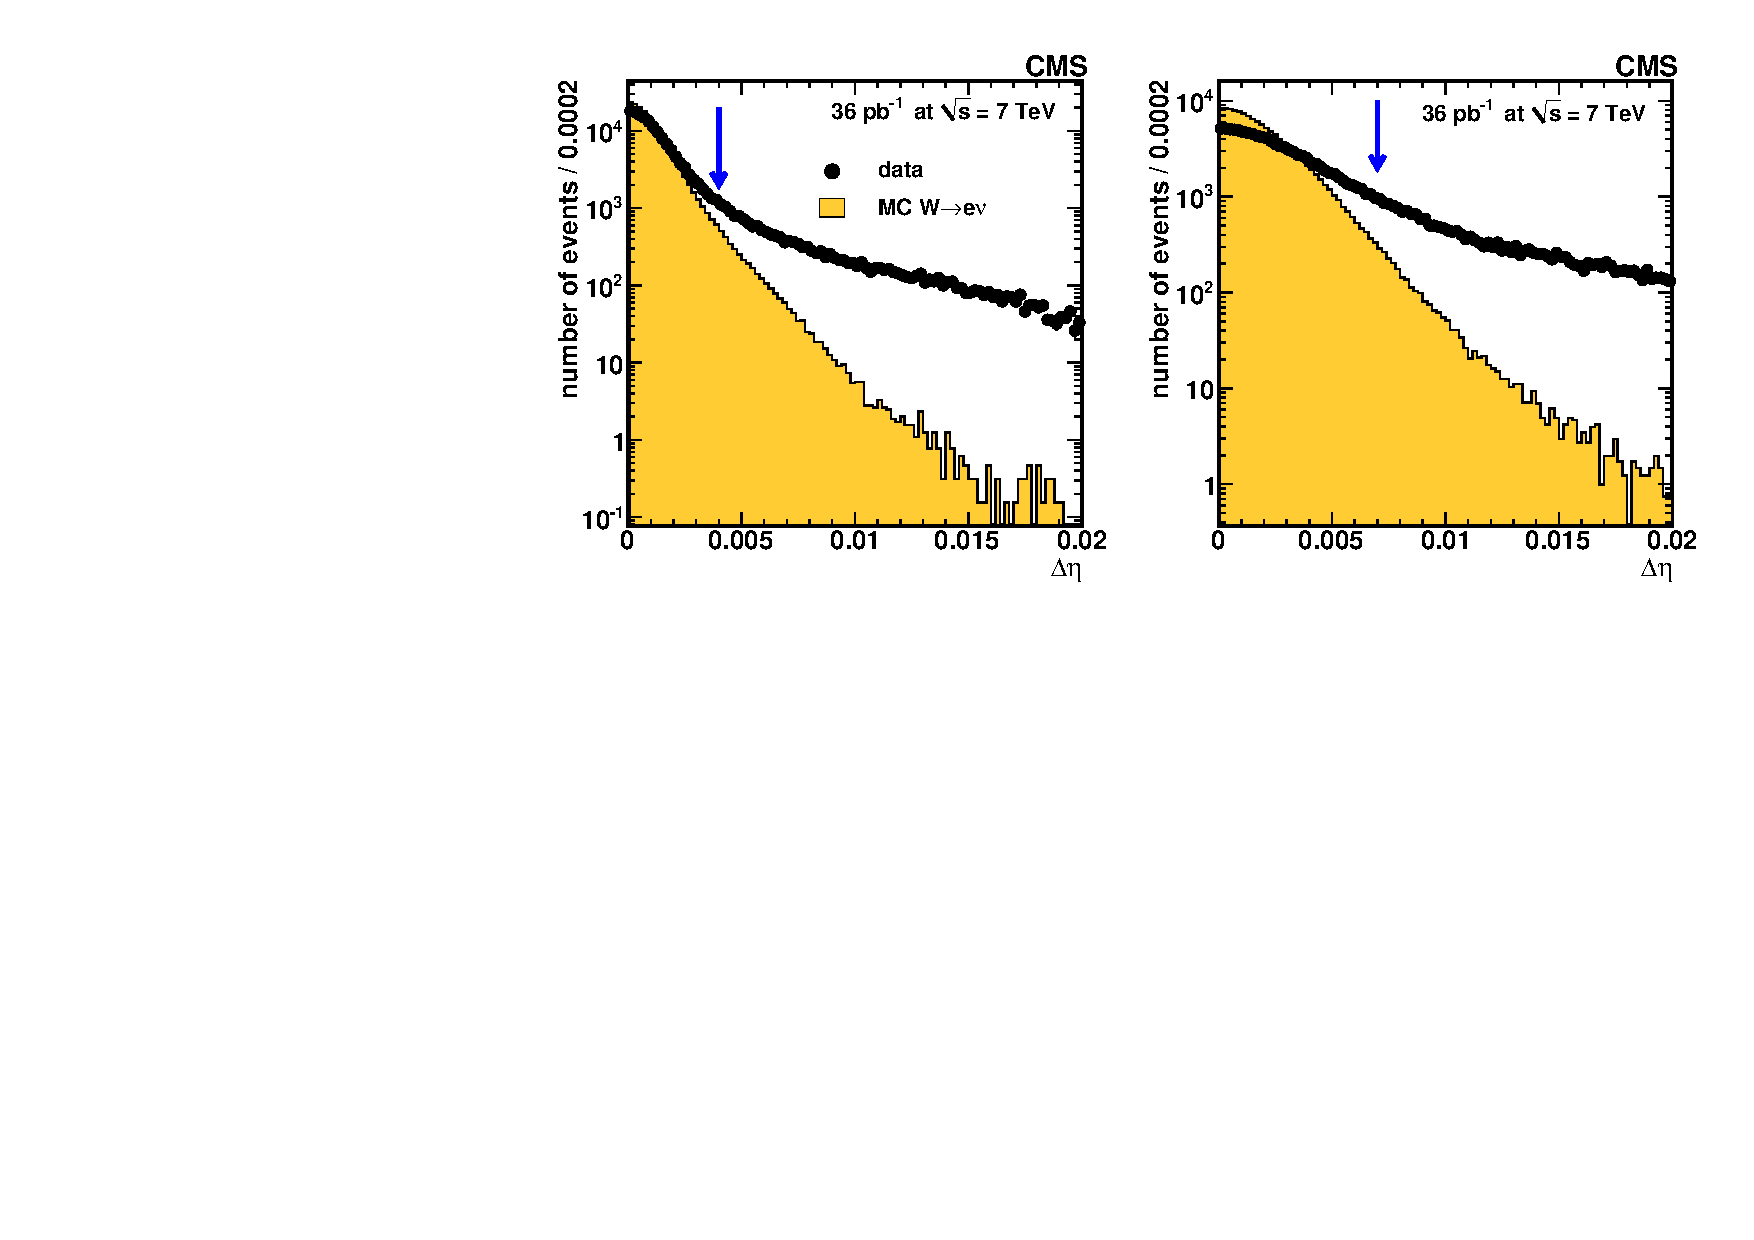
\includegraphics[width=0.68\textwidth]{figs/deta.pdf}
   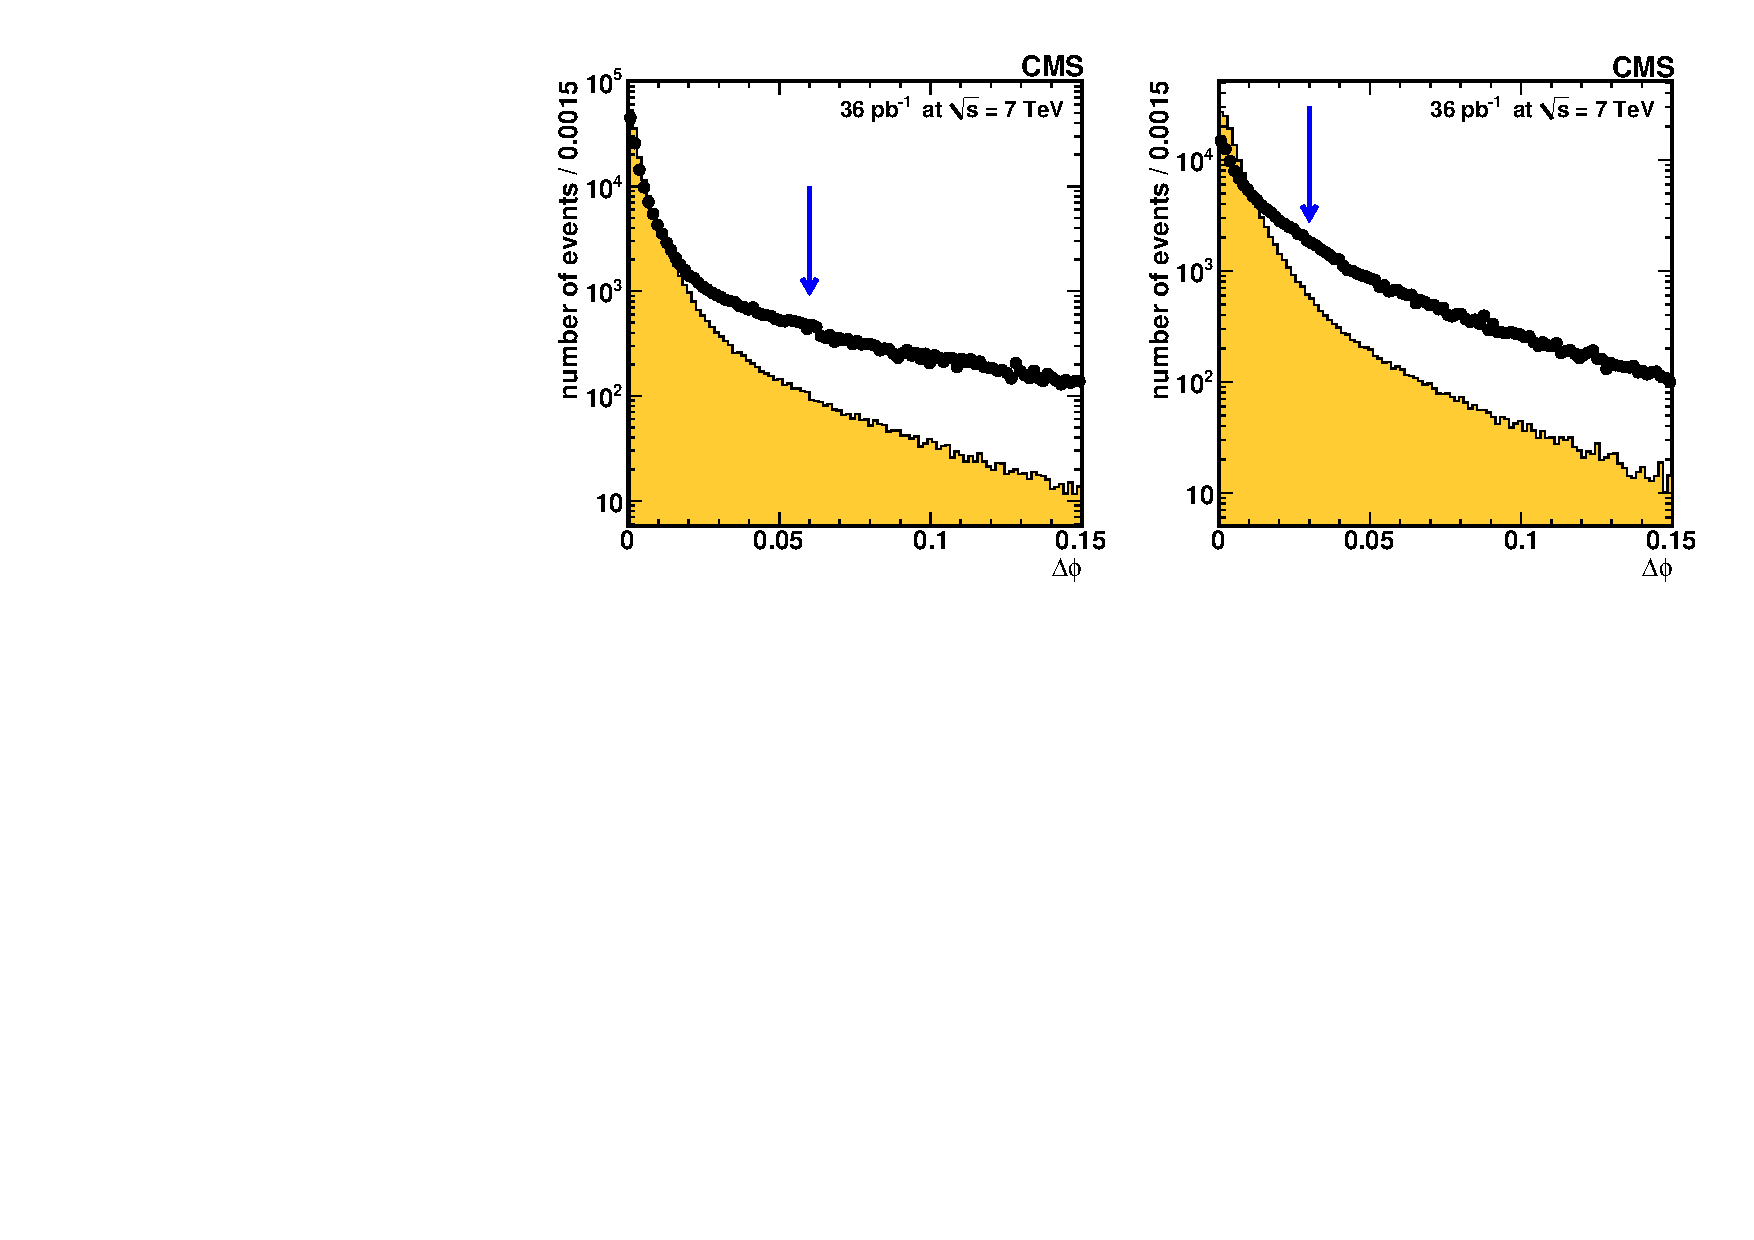
\includegraphics[width=0.68\textwidth]{figs/dphi.pdf}
   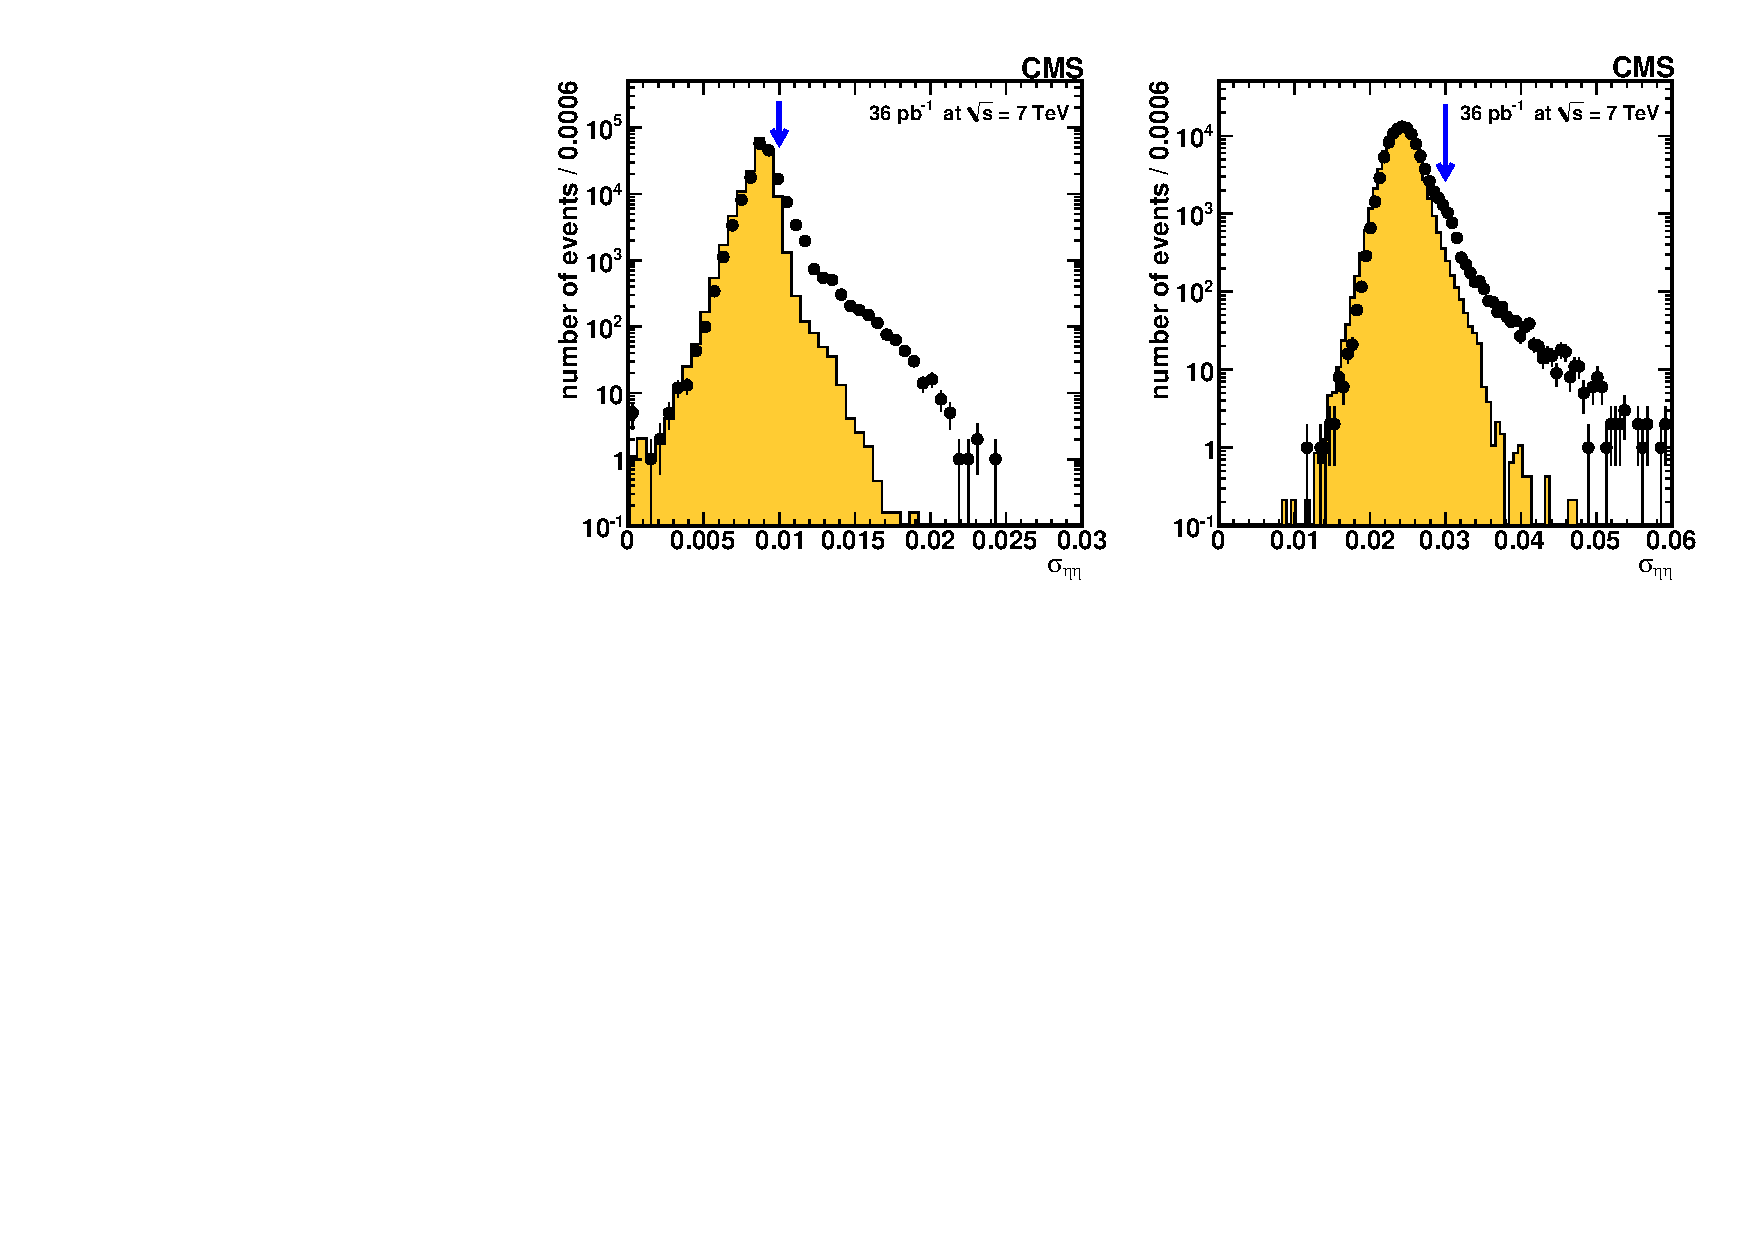
\includegraphics[width=0.68\textwidth]{figs/sihih.pdf}
   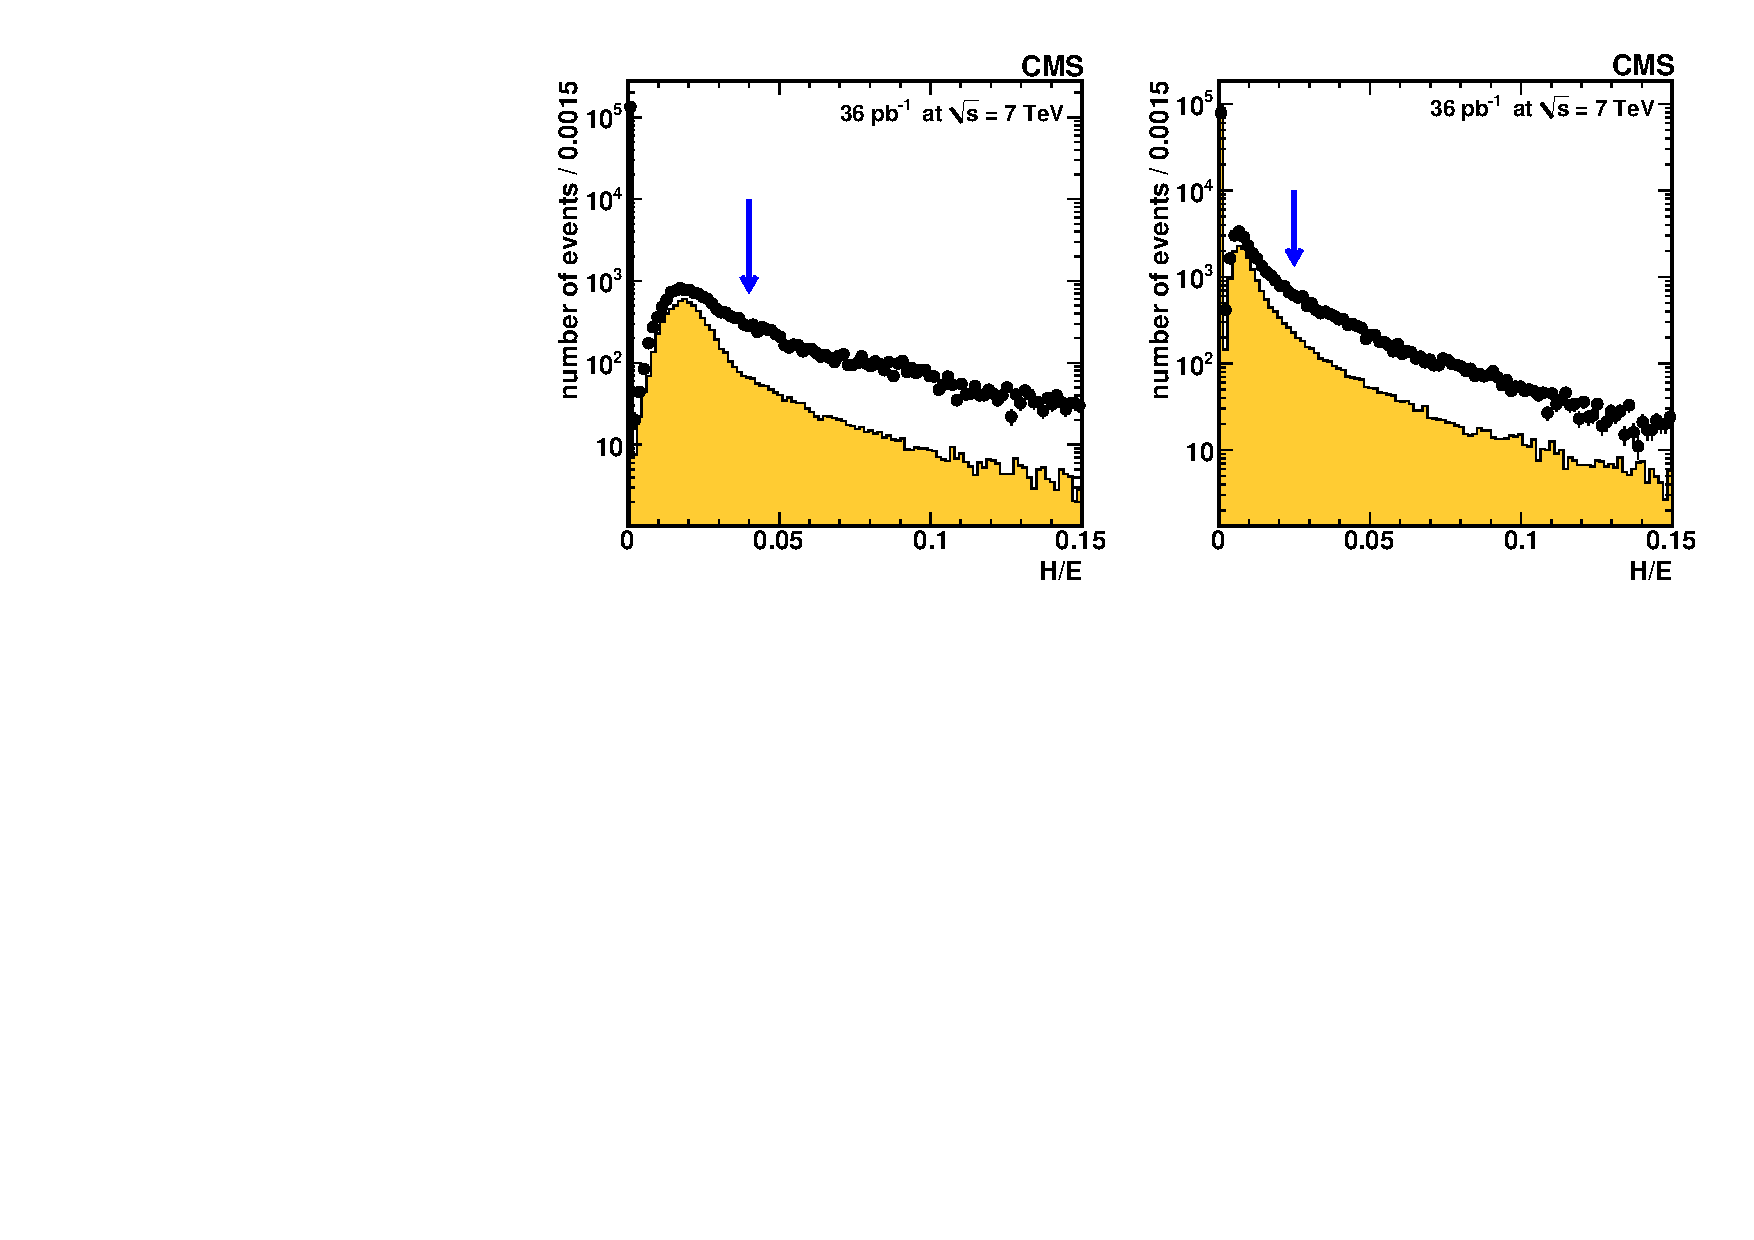
\includegraphics[width=0.68\textwidth]{figs/hoe.pdf}
   \caption{ \label{fig:WenuSelection1}
Distributions of the electron identification variables $\Delta\eta$, $\Delta\phi$, $\sigma_{\eta\eta}$, 
and $H/E$ for data (points with the error bars), for EB (left) and EE (right).
For illustration the simulated $\Wen$ signal (histograms), normalized to the number of events
observed in data, is superimposed.
These distributions are obtained after applying all 
the tight requirements on the selection variables, except that on the presented
variable. The tight requirement on that variable is indicated with an arrow. }
  \end{center}
\end{figure}
%%%%%

%%%%%
\begin{figure}[htbp]
  \begin{center}
   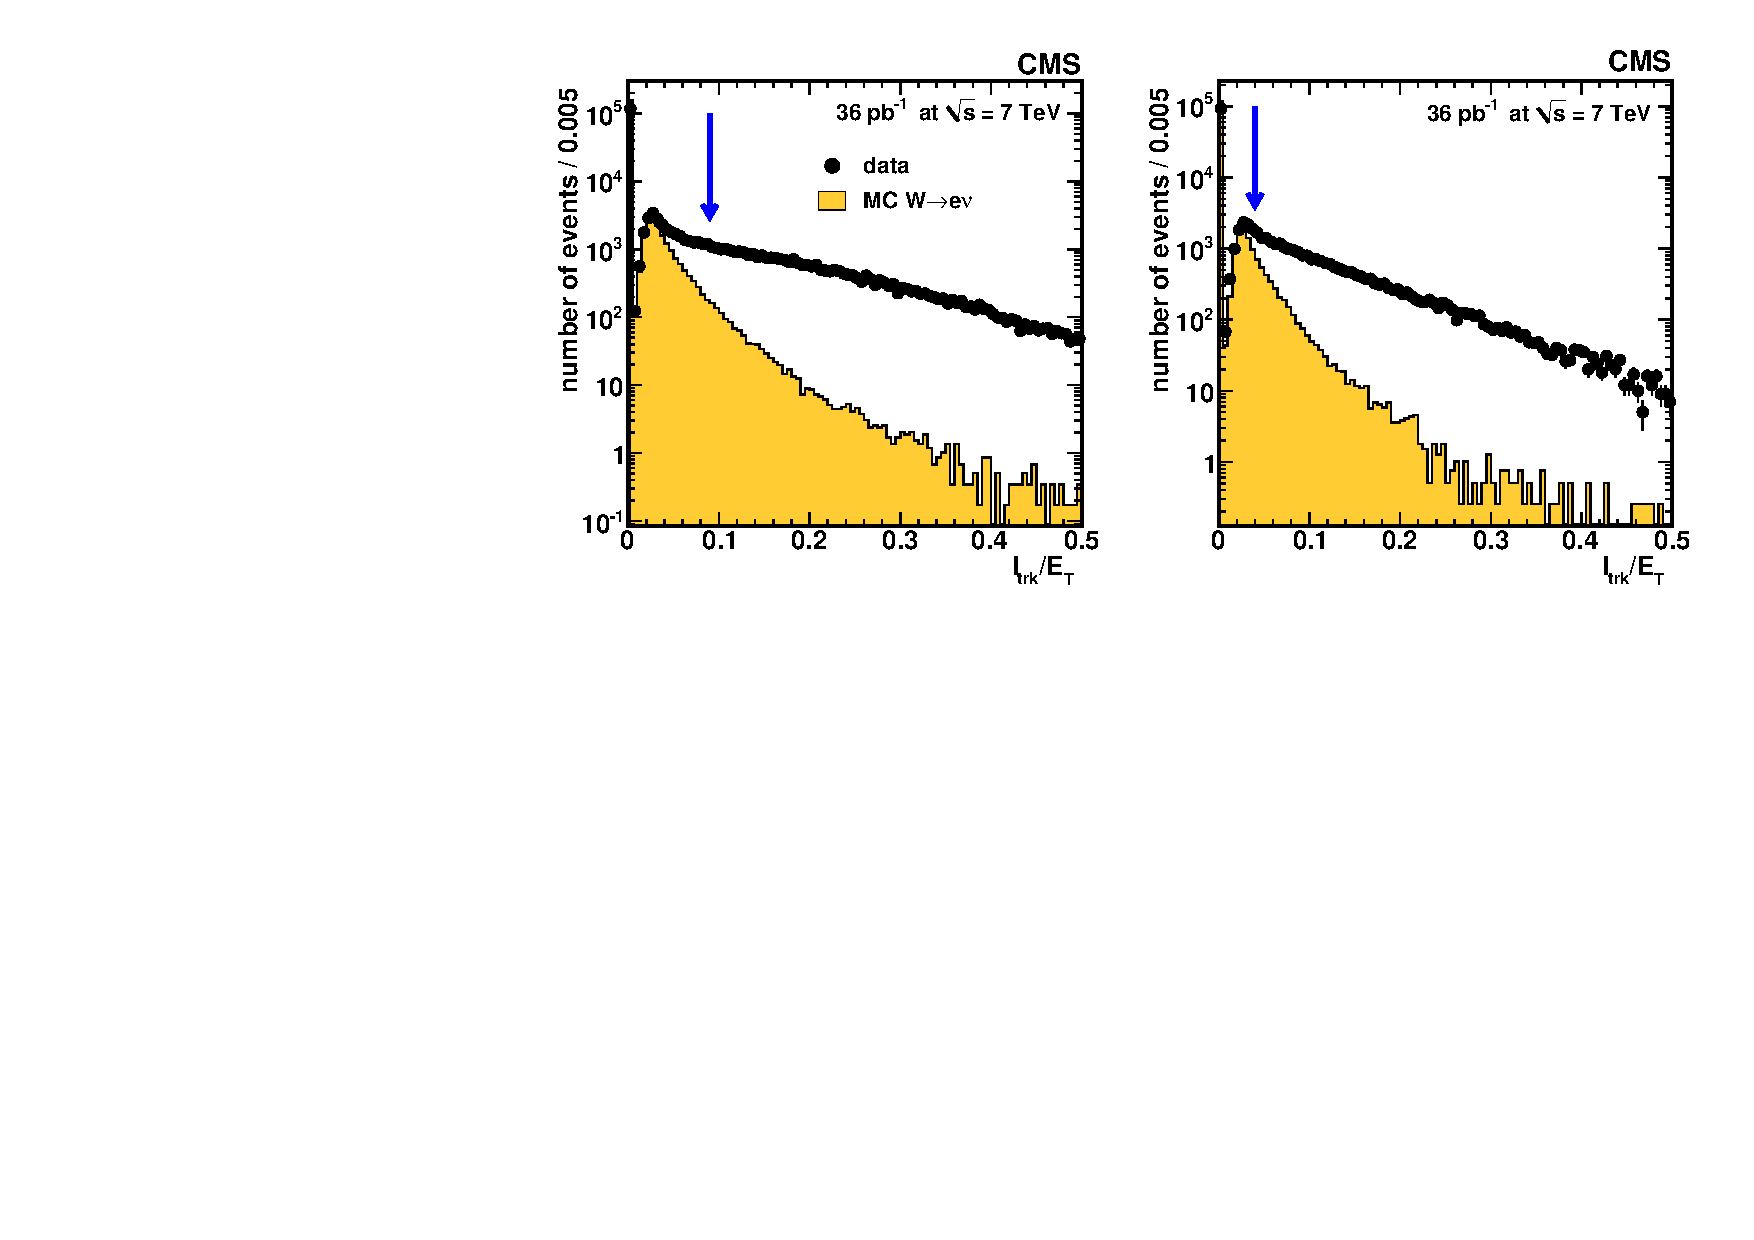
\includegraphics[width=0.68\textwidth]{figs/tkiso.pdf}
   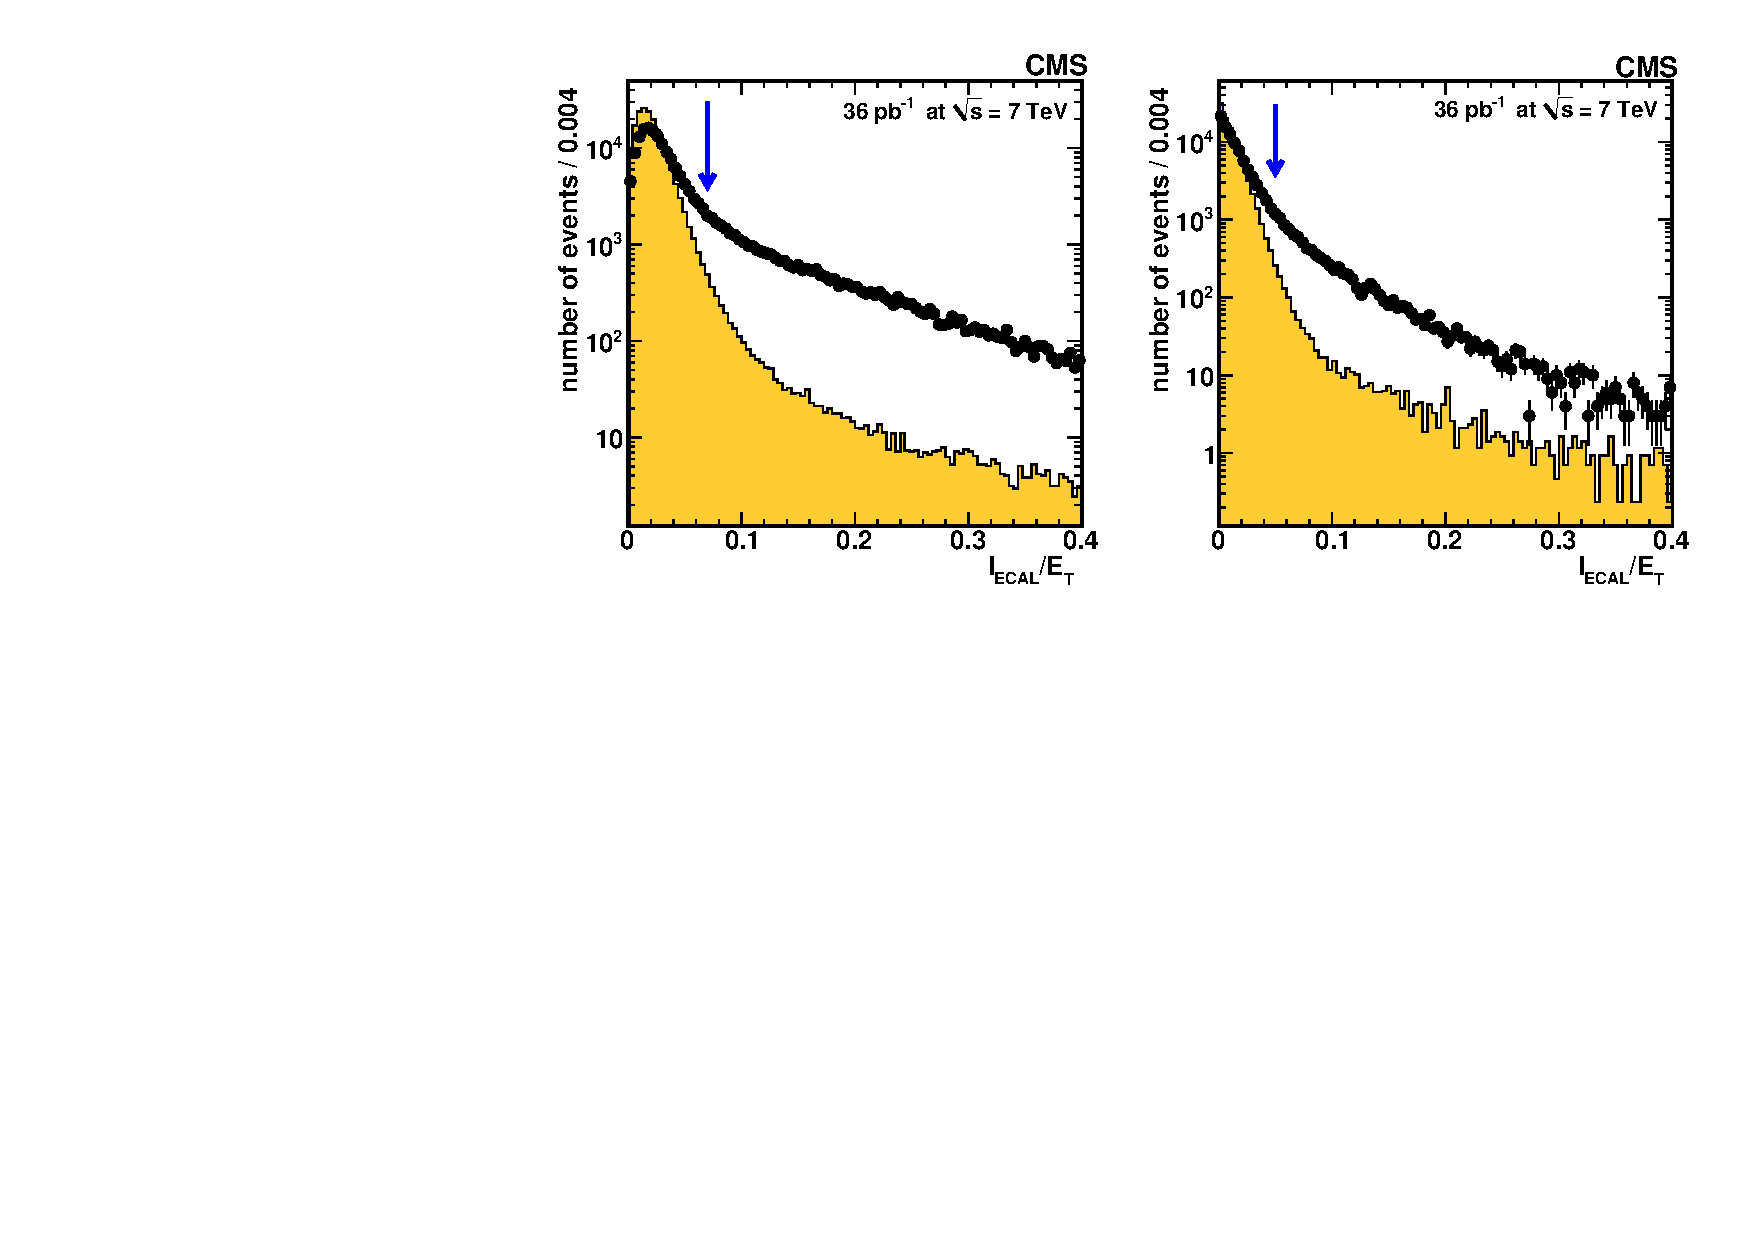
\includegraphics[width=0.68\textwidth]{figs/ecaliso.pdf}
   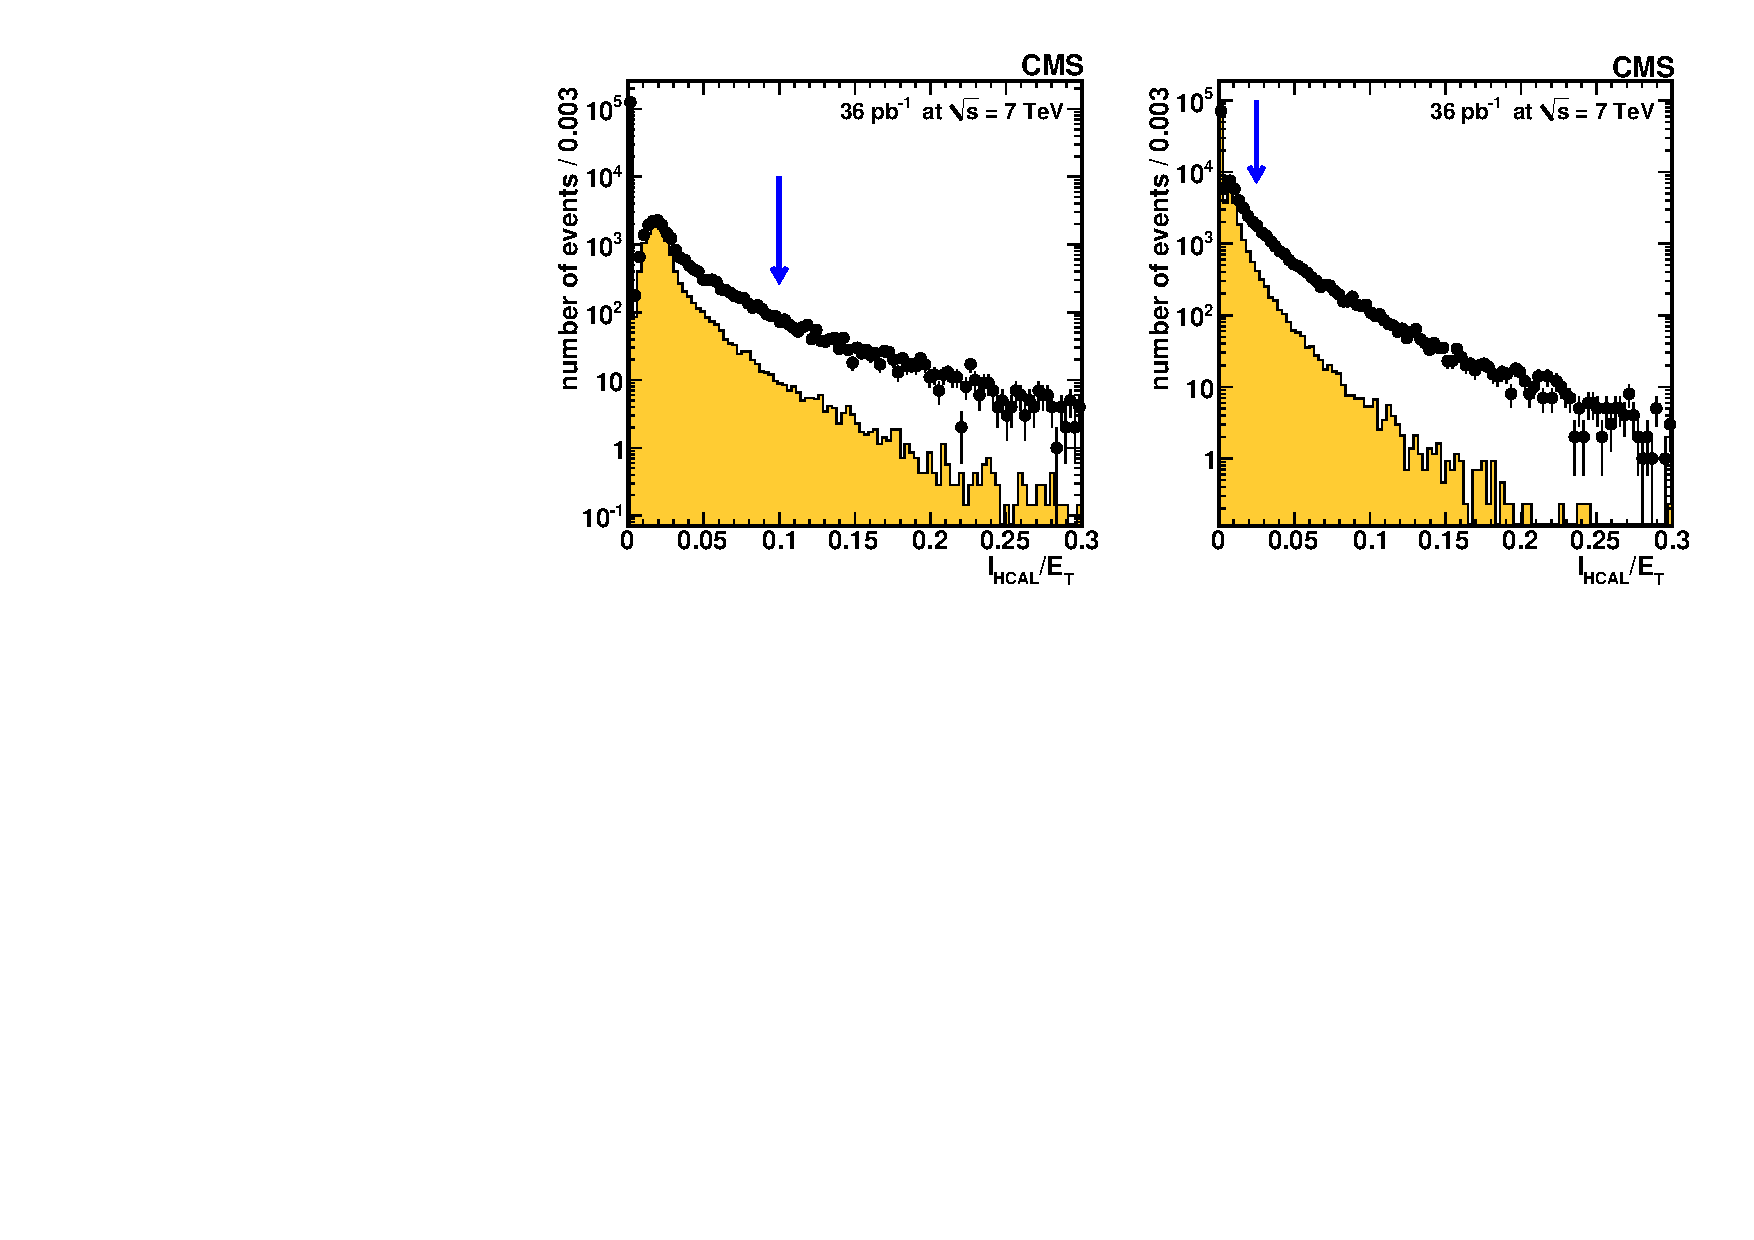
\includegraphics[width=0.68\textwidth]{figs/hcaliso.pdf}
   \caption{ \label{fig:WenuSelection2}
Distributions of the electron isolation variables $\ITRK/\Et$, $\IECAL/\Et$, and $\IHCAL/\Et$
for data (points with the error bars), for EB (left) and EE (right).
For illustration the simulated $\Wen$ signal (histograms), normalized to the number of events
observed in data, is superimposed.
These distributions are obtained after applying all
the tight requirements on the selection variables, except that on the presented
variable. The tight requirement on that variable is indicated with an arrow. }
  \end{center}
\end{figure}
%%%%%

The radiated photons may convert close to the
original electron trajectory, leading to charge misidentification.
Three different methods are used to determine the electron charge. First, the electron 
charge is determined by the signed curvature of the associated GSF track. Second, the charge 
is determined from the associated trajectory reconstructed in the silicon tracker using a 
Kalman Filter algorithm~\cite{KF}. Third, the electron charge is determined based on the azimuthal 
angle between the vector joining the nominal interaction point and the ECAL cluster 
position and the vector joining the nominal interaction point and innermost hit of the GSF track. 
The electron charge is determined from the two out of three charge estimates that are in agreement.
The electron charge misidentification rate is measured in data using the $\Zee$ data
sample to be within 0.1$\%$--1.3$\%$ in EB and 1.4$\%$--2.1$\%$ in EE, increasing with
electron pseudorapidity.


Events are selected if they contain one or two electrons having $\Et>25~\gev$ 
for the $\Wen$ or the $\Zee$ analysis, respectively. 
For the  $\Zee$ selection there is no requirement on the charges of the electrons.
The energy of an electron candidate with $\Et>25~\gev$ is 
determined by the ECAL cluster energy, while its momentum direction is determined by 
that of the associated track. 

Particles misidentified as electrons are suppressed by requiring that the $\eta$ and $\phi$ coordinates
of the track trajectory extrapolated to the ECAL match those
of the ECAL cluster permitting only small differences ($\Delta\eta$, $\Delta\phi$) 
between the coordinates, by requiring a narrow ECAL cluster width in $\eta$ ($\sigma_{\eta\eta}$), 
and by limiting the ratio of the hadronic energy $H$ to the electromagnetic 
energy $E$ measured in a cone of $\Delta R = 0.15$ around the ECAL cluster direction.
More details on the electron identification variables can be found in Refs.~\cite{EGMid,PhotonQCD}. 
Electron isolation is based on requirements on the three isolation 
variables $\IHCAL/\Et$, $\IECAL/\Et$, and $\ITRK/\Et$.

\par
Electrons from photon conversions are suppressed by requiring the 
reconstructed electron track to have at least one hit in the innermost pixel layer.
Furthermore, electrons are
rejected when a partner track is found that is consistent with a
photon conversion, based on the opening angle and the separation in
the transverse plane at the point where the electron and partner
tracks are parallel.

The electron selection criteria were obtained
by optimizing signal and background levels according to
simulation-based studies. The optimization was done for EB
and EE separately.  

Two sets of electron selection criteria are considered: 
a tight one and a loose one.
Their efficiencies, from simulation studies based on $\Wen$ events, are
approximately 80$\%$ and 95$\%$, respectively. These efficiencies correspond 
to reconstructed electrons within the geometrical and kinematic 
acceptance, which is defined in Section~\ref{sec:acceptance}.  
The tight selection criteria give a purer sample of prompt 
electrons and are used for both the $\Wen$ and $\Zee$ analyses.
The virtue of this choice is to have consistent electron definitions 
for both analyses, simplifying the treatment of systematic 
uncertainties in the $\mathrm{W}/\mathrm{Z}$ ratio measurement. 
In addition, the tight working point, applied to both electrons
in the $\Zee$ analysis, reduces the QCD backgrounds to a negligible level.
%%The values of the cuts for the tight and "loose" selection sets are 
%%listed in Table~\ref{tab:electron_cuts}.
%%%%% GD
Distributions of the selection variables are shown in Figs.~\ref{fig:WenuSelection1}
and~\ref{fig:WenuSelection2}.
The plots show the distribution of data together with the simulated signal 
normalized to the same number of events as the data, after applying all 
the tight requirements on the selection variables except the requirement on the displayed
variable. 
%The tight cut on that variable is shown with a vertical line.



For the W analysis, an event is also rejected if there is a second electron 
that passes the loose selection with $\Et > 20~\gev$. This requirement reduces
the contamination from DY events.  
The number of $\Wen$ candidate events selected in the data sample is 
$\WEISAMPLE$, with $\WEPSAMPLE$ positrons and $\WEMSAMPLE$ electrons.

For the Z analysis, two electrons are required within the ECAL acceptance, 
both with $\Et > 25~\gev$ and both satisfying the tight electron selection. 
Events in the dielectron mass region of $60 < m_{\mathrm{ee}} < 120$~GeV are counted.
These requirements select $\ZEESAMPLE$ events.



% \begin{table}[htb]
% \caption{Selection cuts for electrons.}
% \label{tab:electron_cuts}
% \begin{center}
% \begin{tabular}{ | l || c | c || c | c |}
% \hline
%           & \multicolumn{2}{| c ||}{"Loose" e} & \multicolumn{2}{| c |}{tight e} \\
% \hline
%                          & Barrel & Endcap & Barrel & Endcap \\
% \hline \hline
%    $\ITRK/\Et$             & 0.15   & 0.08   & 0.09   & 0.04   \\
% \hline
%    $\IECAL/\Et$              & 2.0    & 0.06   & 0.07   & 0.05   \\
% \hline
%    $\IHCAL/\Et$              & 0.12   & 0.05   & 0.10   & 0.025  \\
% \hline
%    Missing hits $\leq$    & 1      & 1      & 0      & 0      \\
% \hline
%    Dcot                  & $-$    & $-$    & 0.02   & 0.02   \\
% \hline
%    Dist                  & $-$    & $-$    & 0.02   & 0.02   \\
% \hline
%    $\sigma_{\eta\eta}$   & 0.01   & 0.03   & 0.01   & 0.03   \\
% \hline
%    \DP                    & $-$    & $-$    & 0.06   & 0.03   \\
% \hline
%    \DE                    & 0.007  & 0.01   & 0.004  & 0.007  \\
% \hline
%    $H/E$                  & 0.15   & 0.07   & 0.04   & 0.025  \\
% \hline
% \end{tabular}
% \end{center}
% \end{table}






%%\subsection{Muons \label{sec:muonId}}

%Muon used in this analysis are selected according to the
%quality criteria studies in
%Events with high-$\Pt$ muons are recorded online using the Level-1 muon
%trigger and the High-Level Trigger (HLT), which requires muons within $|\eta| < 2.1$ and
%with a thresholds of $\Pt>9 \GeVc$ or $\Pt>15 \GeVc$, according to the running periods. 
Muons must be identified by two different algorithms~\cite{MUONPAS}: one proceeds from 
the inner tracker outwards (``tracker muons''), the other one starts from 
segments in the muon chambers and proceeds inwards (``global muons''). 
Decays in flight of hadrons and punch-through are reducing a cut of $\chi^2/ndof < 10$ 
on a global fit containing tracker and muon detector hits. 
In order to ensure a precise estimate of momentum and impact parameter 
%(the muon momentum resolution is dominated by the inner tracker detector
%for the tranverse momentum range interesting for this measurement)
only tracks with more than 10 hits and at least one hit in the pixel detector are used. 
We require at least two levels of muon stations in the measurement, 
to ensures a good quality momentum estimate at trigger level, and
to further suppresses remaining fake muon candidates.
%For the $\Zmm$ analysis we minimize the cross-corrlation between tracker and muon 
%detectors by drop the $\chi^2/{\mathrm{ndof}}$ and 
%the request that the muon is found by the tracker algorithm.
Cosmics are rejected by requiring a transverse impact parameter distance to the beam spot
position of less than 2 mm.

%\section{Missing Transverse Energy\label{sec:MET}}
An accurate $\MET$ measurement is essential for distinguishing
$\Wo$ signal from QCD backgrounds. We use $\MET$ estimate provided
by the Particle Flow (PF) algorithm which showed the best performance for the
CMS detector. Details on Particle Flow $\MET$ are provided in Ref.~\cite{PFMET}. 
\par
We have very good agreement of the $\MET$
distributions in $\Wln$ in data and simulation~\cite{metPAS}.
\par
The $\MET$ is computed as the vector sum of all PF objects.
The resolution for inclusive multi-jet samples and for
$\Wln$ events is well reproduced by the 
simulation.  A modest broadening of about $10\%$ is observed 
when there is more than one primary vertex; this occurs in less 
than $40\%$ of the events and has a negligible impact on the
extraction of the $W$ yields described below.


\section{Lepton Selection Efficiencies\label{sec:leptonSel}}
\par
The efficiencies for lepton reconstruction, identification,
isolation and trigger efficiencies are obtained from data.
Correction factors are the ratios of efficiencies extracted from data and simulations 
($\rho = {\epsilon_{\mathrm{data}}}/{\epsilon_{\mathrm{MC}}}$) 
with a tag-and-probe method exercised on $\Zll$ samples in both data and simulation.
%This procedure adequately removes any systematic uncertainties coming from imperfections in
%the simulation, even though the kinematic distributions
%of leptons in the $\Zll$ sample differ slightly from those
%in the selected $\Wln$ sample.
The tag-and-probe sample for the measurement of a given efficiency
contains events selected with two lepton candidates.
One lepton candidate, called the ``tag,'' satisfies
tight identification and isolation requirements. The other
lepton candidate, called the ``probe,'' is selected with
criteria that depend on the efficiency being measured.
The invariant mass of the tag and probe lepton candidates
must fall in the range $60$--$120~\GeV$.
%The signal yields are obtained for two exclusive subsamples of events
%in which the probe lepton passes or fails the selection criteria considered.
%Fits are performed to the invariant-mass distributions
%of the pass and fail subsamples, including a term that
%accounts for the background.
%The measured efficiency is
%deduced from the relative level of signal in the pass and fail subsamples;
%its uncertainty includes a systematic contribution from the fitting
%procedure.
%\par
%The correction factors are obtained as
%ratios of tag-and-probe efficiencies for
%the data and for the simulation.  They are used to compute
%the signal selection efficiency ratios $\RHO{}$, and
%their uncertainties are  propagated as systematic uncertainties
%on these quantities,
%except in the $\Zmm$ analysis, for which the efficiencies and yields
%are determined simultaneously.


\subsection{Electrons}
\label{sec:ELEefficiencies}

%The overall electron efficiency is the product of
%three terms: the reconstruction efficiency (GSF tracking),
%the selection efficiency (identification and isolation criteria),
%and the trigger efficiency (L1+HLT), taken in this order.
As mentioned in the previous section, 
the tight electron selection is considered for both the W and Z analyses, so 
the overall efficiency can be written as
\begin{equation}
  \EPS{all} = \EPS{rec}\, \EPS{tight}\, \EPS{trg}.
\label{eq:e-eff}
\end{equation}
The reconstruction efficiency $\EPS{rec}$ is relative to ECAL clusters
within the ECAL acceptance, the selection efficiency $\EPS{tight}$ is relative to GSF electrons
within the acceptance, and the trigger efficiency $\EPS{trg}$ is relative to electrons
satisfying the tight selection criteria.

\par
All the efficiencies are determined by the \TNP technique.
%The tag electron is required to pass the tight electron
%identification criteria. 
Selections with different criteria have been 
tried on the tag electron. It was found that the estimated efficiencies are 
insensitive to the tag selection definition. 
The invariant mass of the \TNP pair
is required to be within the window $60<m_{\mathrm{ee}}<120~\GeV$.
%,ensuring high purity of the probe sample. 
No opposite-charge requirement is enforced.
%The measured efficiency for a given selection
%is the fraction of probes passing the selection.

The number of probes passing and failing the selection is
determined from fits to the invariant mass distribution,
with signal and background components.
Estimated backgrounds, mostly from QCD multijet processes, are in most cases
at the percent level of the overall sample, but can be larger in subsamples
where the probe fails a selection, hence the importance of background
modeling. The signal shape is a Breit--Wigner with nominal Z mass and width convolved with an
asymmetric resolution function (Crystal Ball~\cite{CrystalBall}) with floating parameters.  The
background is modeled by an exponential. Systematic uncertainties that depend on the efficiency
under study are determined by considering alternative signal and background shape models.
Details can be found in Section~\ref{sec:systematics}. 

%A systematic error which depends on the efficiency
%under study is determined by considering alternative background models like power-low or error function
%multiplied with an exponential. The size of the background systematic is 0.3$\%$ for the electron
%identification efficiencies and 1.0$\%$ for electron reconstruction efficiency. The estimation
%of the trigger efficiency is considered to be background free.

%
% GD too technical to be interesting
%
%For this selection, only the charge of the probe is considered except for the
%determination of the reconstruction efficiency, where the probe (which is an
%ECAL cluster) is assigned the charge opposite to that of the tag.
%For the determination of the reconstruction efficiency,
%the probe is an ECAL cluster within ECAL acceptance.
%To reduce the background level, and only in that case, we
%require the ECAL cluster to pass a loose $H/E<0.15$ 
%requirement for both EB and EE which is shown from
%simulations to be almost uncorrelated with the reconstruction efficiency.
%The reconstruction efficiencies have been independently estimated by varying 
%the ECAL cluster "cleaning" criteria or without any cleaning cuts giving 
%consistent results with the first method.


%\begin{figure}[htbp]
%\begin{center}
% \begin{minipage}[Reconstruction]{0.32\textwidth}
%  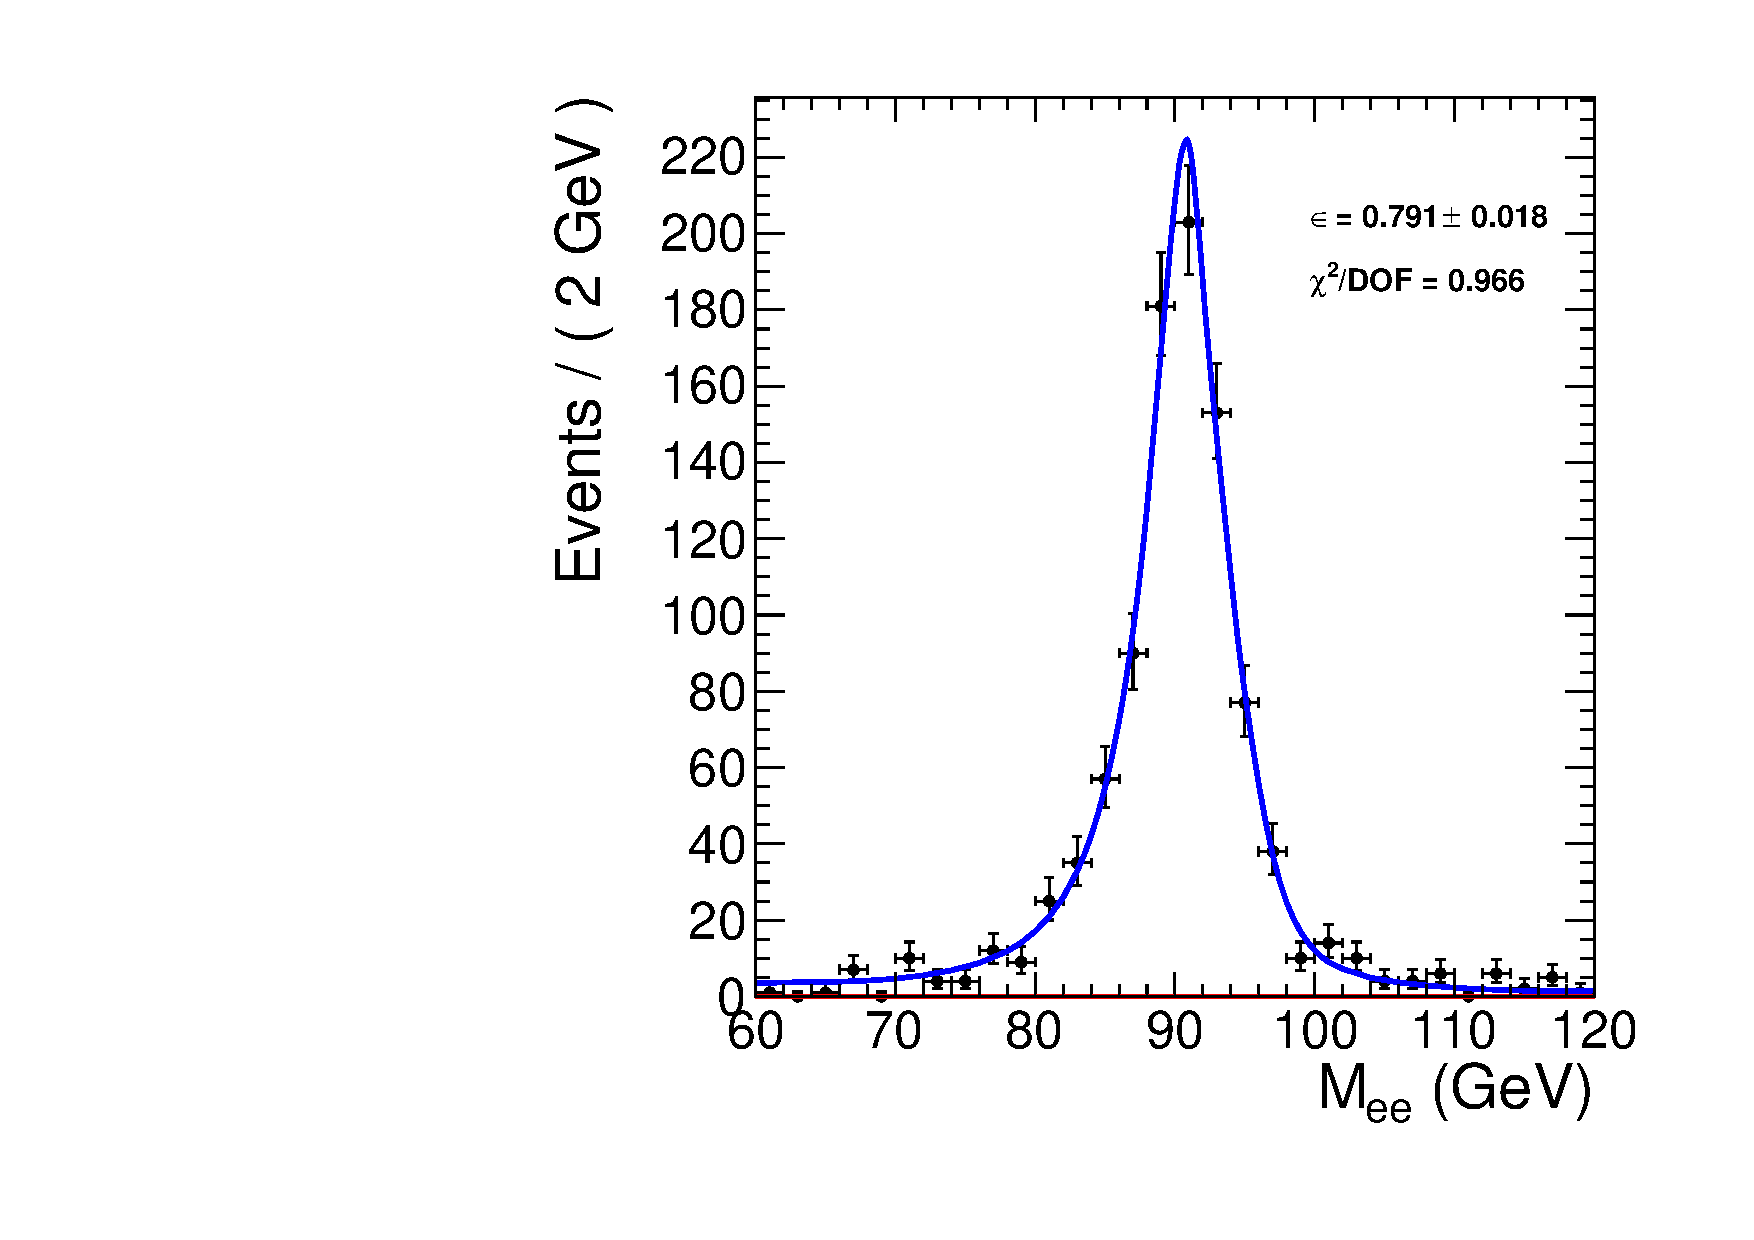
\includegraphics[width=1.0\textwidth]{figs/tpHistos_ID80_eb_pass.pdf}
%  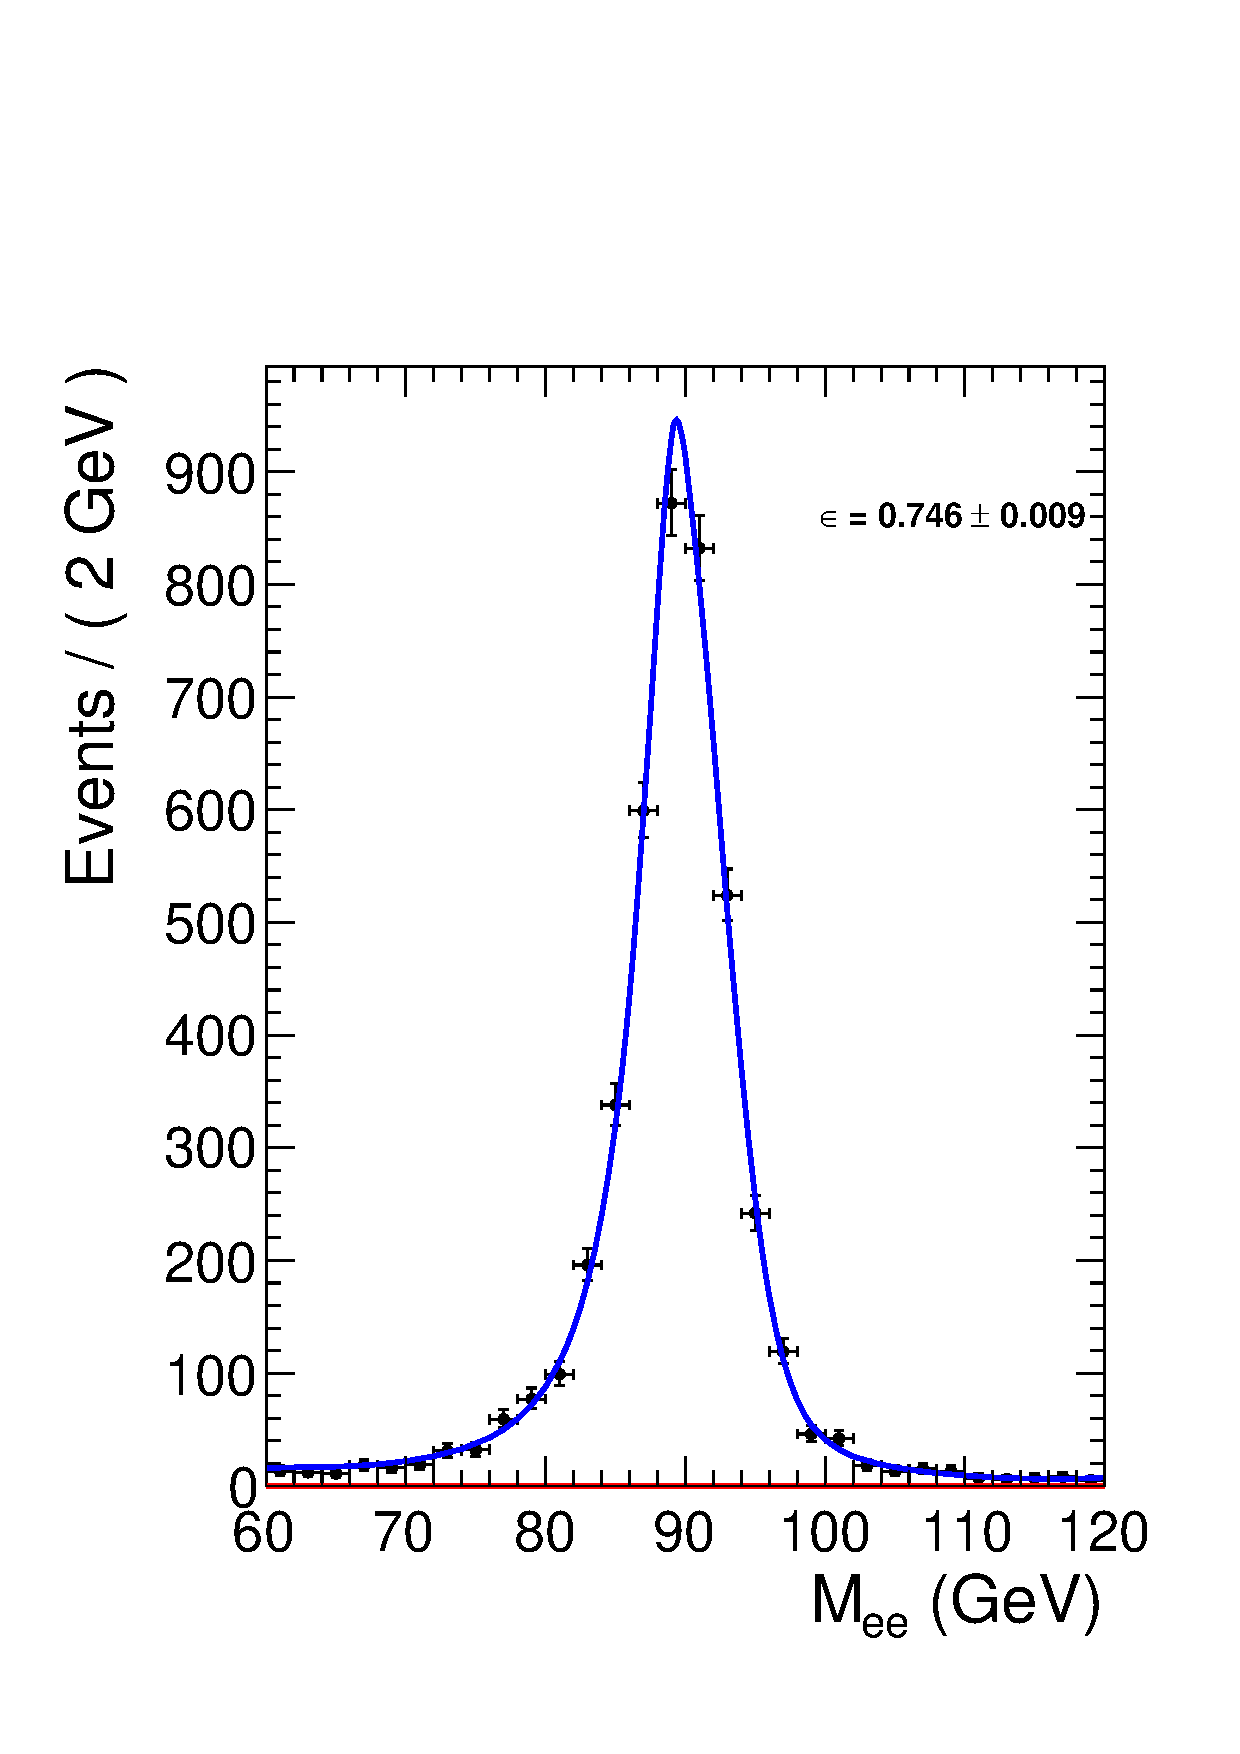
\includegraphics[width=1.0\textwidth]{figs/tpHistos_ID80_ee_pass.pdf}
% \end{minipage}
% \begin{minipage}[WP80]{0.32\textwidth}
%  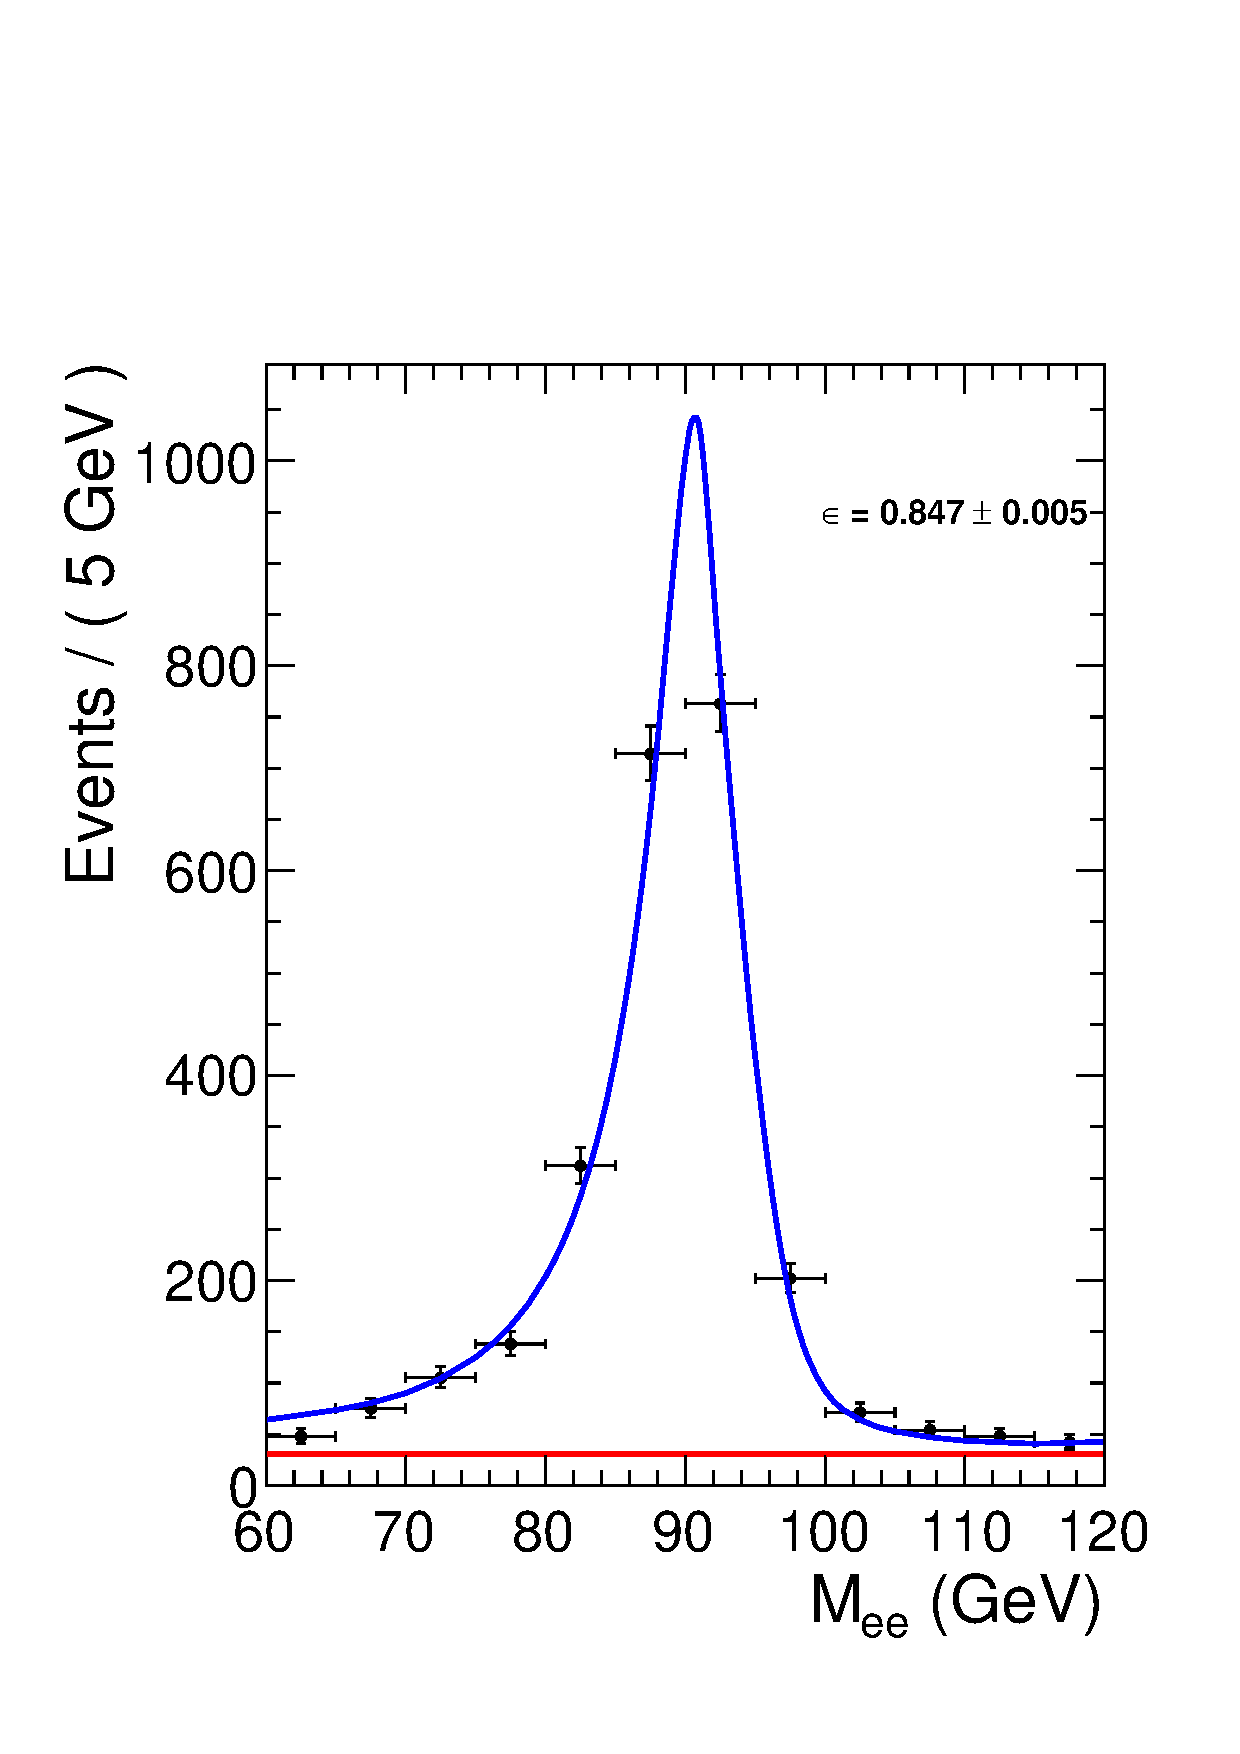
\includegraphics[width=1.0\textwidth]{figs/tpHistos_ID80_eb_fail.pdf}
%  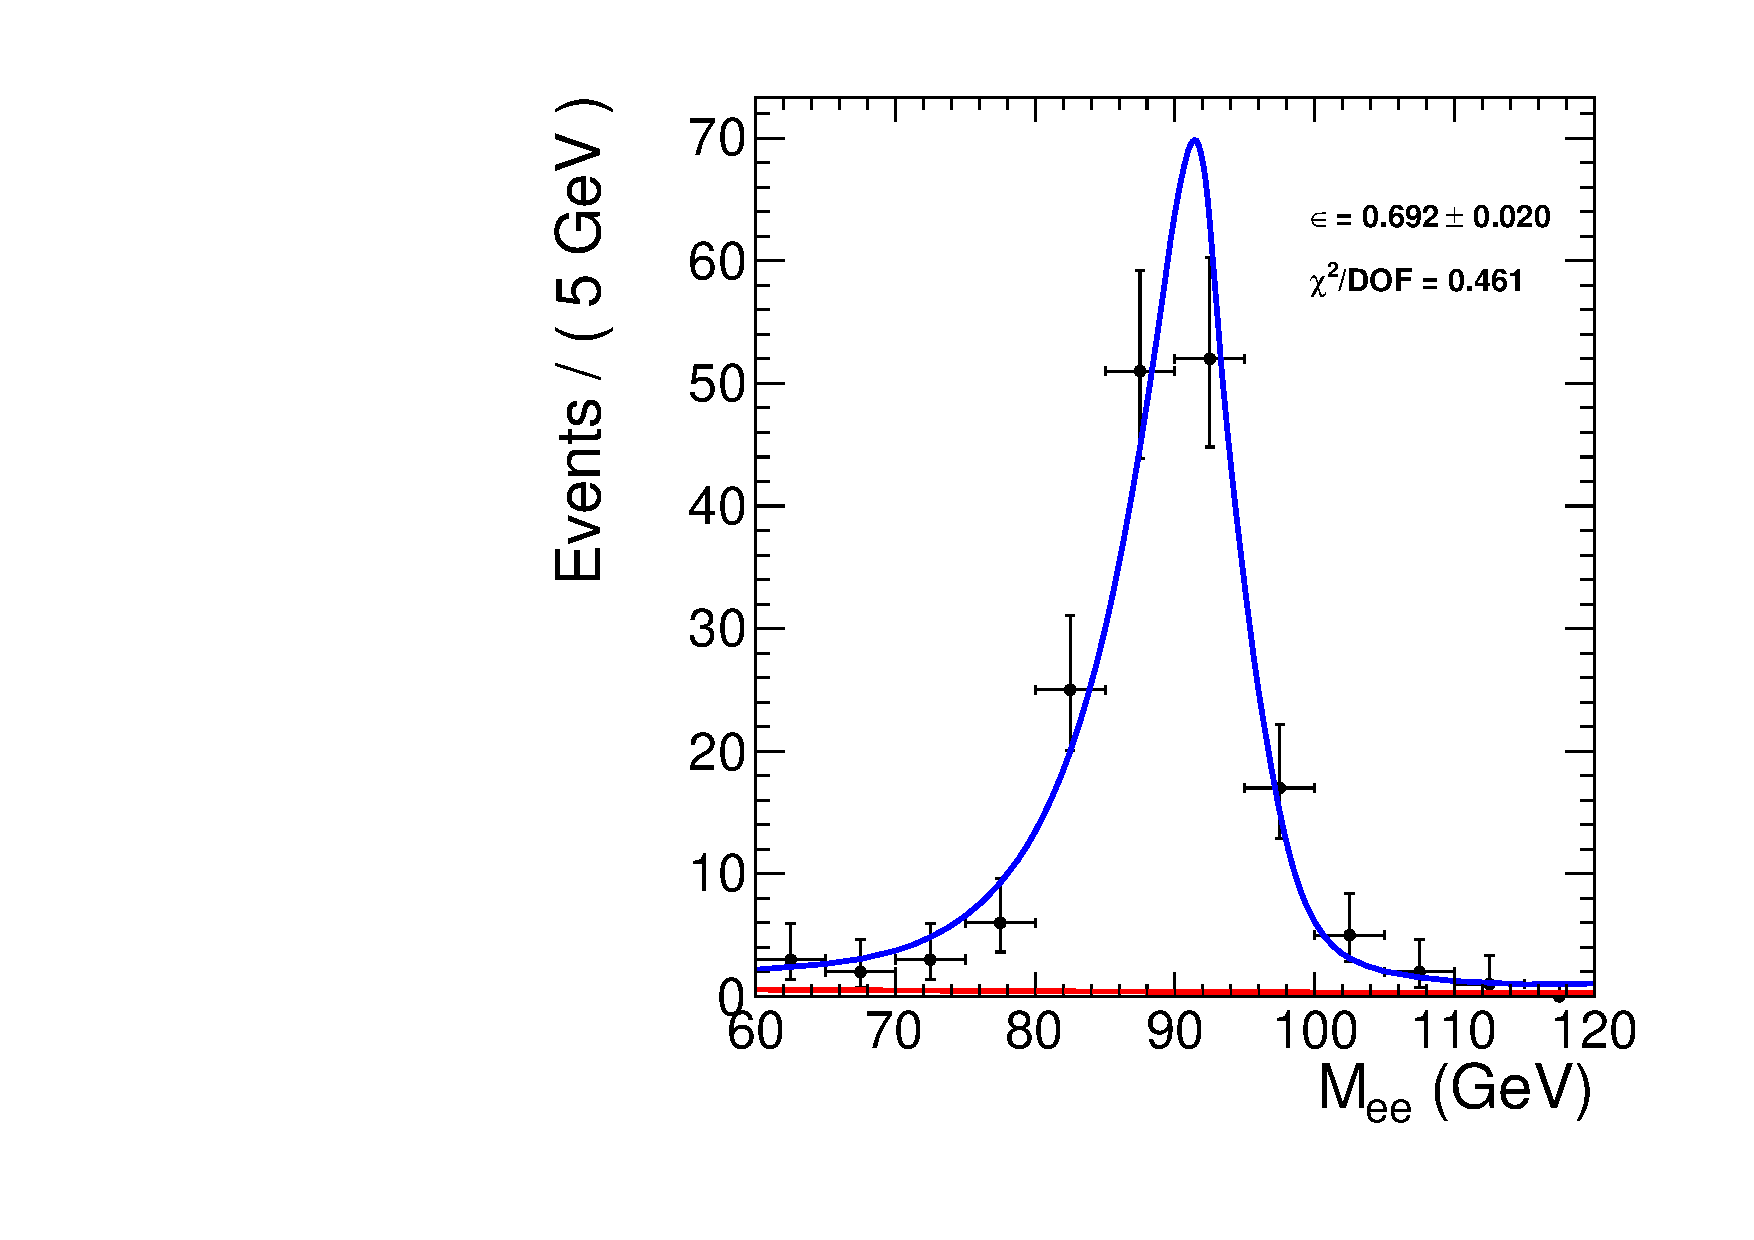
\includegraphics[width=1.0\textwidth]{figs/tpHistos_ID80_ee_fail.pdf}
% \end{minipage}
%% \begin{minipage}[W80toTrigger]{0.32\textwidth}
%%  \includegraphics[width=1.0\textwidth]{figs/TNPe_fake.png}
%%  \includegraphics[width=1.0\textwidth]{figs/TNPe_fake.png}
%% \end{minipage}
% \end{center}
%\caption{Extraction of \TNP efficiencies in the data from fits
%to the dielectron mass distributions for passing (upper row) and failing (lower row) probes:
%GSF-electron $\to$ tight selection for ECAL Barrel (left column) and ECAL Endcaps (right column). 
%The red line represents the background estimation.
%\label{fig:e-TNP}}
%\end{figure}
%Examples of \TNP fits on the data are given in Fig.~\ref{fig:e-TNP}
%for illustration.
%% can't cite an AN
%% All the details of the \TNP fits can be found in~\cite{CMS_AN_2010-323}.


%In addition to efficiencies, we report data/MC efficiency
%ratios $\rhoeff$, also called data/MC correction factors:
%\begin{equation}
%  \rho_{\textrm{eff-X}} = \frac{\EPS{TNP-X}(\textrm{data})}{\EPS{TNP-X}(\textrm{MC})}  \ \ \ 
%\textrm{and} \ \ \ \EPS{X} = \EPS{MC-X} \times \rho_{\textrm{eff-X}} ,
%\end{equation}
%where $\EPS{X}$ is the final electron efficiency
%and $\EPS{MC-X}$, the ``true''
%MC efficiency, for selection $X$ (reco, tight selection, HLT or overall).

The \TNP event selection efficiencies in the simulation 
are determined from large samples of signal events with no
background added.

%The main reason for considering data/MC correction factors rather
%than absolute efficiencies is that some biases cancel in the ratio.
%One bias that affects the $W$ analysis comes from the fact that,
%due limited statistics, we consider only two bins
%in pseudorapidity (EB and EE). In each bin efficiencies are weighted
%by the pseudorapidity distribution of electrons from Z decays,
%which is different from that of electrons from W$^+$ or W$^-$ decays.
%Hence, any $\eta$ dependence of the efficiency within the bin induces
%a bias, which is expected to cancel in the ratio (assuming that
%the dependence is roughly reproduced in the simulation).

The \TNP efficiencies are measured for the EB and EE electrons separately.
Tag-and-probe efficiencies are also determined separately by charge, 
to be used in the measurements of the W$^+$ and W$^-$ cross sections and their ratio.
%For this selection, only the charge of the probe is considered except for the
%determination of the reconstruction efficiency, where the probe (which is an
%ECAL cluster) is assigned the charge opposite to that of the tag.
%Tag-and-probe electron efficiencies, for the data and the Monte Carlo 
%simulation, and efficiency correction factors, are summarized in 
%Table~\ref{tab:e-eff-summary}. 
Inclusive efficiencies and correction factors are summarized in 
Table~\ref{tab:e-eff-summary}. The \TNP measurements of the efficiencies 
on the right-hand side of Eq.~(\ref{eq:e-eff})
are denoted as $\EPSTNPREC$, $\EPS{\tnp-tight}$, and $\EPSTNPTRG$.

%--------------------------------------------------
\begin{table}[htbp] %
\begin{center}
\caption[.]{\label{tab:e-eff-summary}
Tag-and-probe efficiencies in data and simulation, and the correction factors
used in the electron channels for the barrel (EB) and endcaps (EE). The combined statistical and systematic 
uncertainties are quoted. }
\begin{tabular}{|l|c|c|c|}
\hline
Efficiency & Data & Simulation & Data/simulation ($\rhoeff$) \\
\hline
\hline
\multicolumn{4}{|c|}{EB} \\
\hline
 \EPS{\tnp-rec}      & \WPWIEBEFFRECO  & \WPWIEBMCRECO & \WPWIEBRRECO \\
 \EPS{\tnp-tight}    & \WPWIEBEFFID    & \WPWIEBMCID   & \WPWIEBRID   \\
 \EPS{\tnp-trg}      & \WPWIEBEFFHLT   & \WPWIEBMCHLT  & \WPWIEBRHLT  \\
\hline
 \EPS{\tnp-all}  & \WPWIEBEFF  & \WPWIEBMC & \WPWIEBR \\
\hline
\hline
\multicolumn{4}{|c|}{EE} \\
\hline
 \EPS{\tnp-rec}       & \WPWIEEEFFRECO  & \WPWIEEMCRECO & \WPWIEERRECO \\
 \EPS{\tnp-tight}    & \WPWIEEEFFID    & \WPWIEEMCID   & \WPWIEERID   \\
 \EPS{\tnp-trg} & \WPWIEEEFFHLT   & \WPWIEEMCHLT  & \WPWIEERHLT  \\
\hline
 \EPS{\tnp-all}  & \WPWIEEEFF  & \WPWIEEMC & \WPWIEER \\
\hline
\end{tabular}
\end{center}
\end{table}


\par
Event selection efficiencies are measured with respect to the W events
within the ECAL acceptance.
Simulation efficiencies estimated from {\sc POWHEG} $\Wo$ samples 
are shown in Table~\ref{tab:el-Weff}.
These are efficiencies at the event level,
e.g.: they include efficiency loss due to the second electron veto.  
Given the acceptances listed in Table~\ref{tab:WZlaccgen} and the \TNP 
efficiencies listed in Table~\ref{tab:e-eff-summary},
the overall efficiency correction factors for electrons from $\Wo$ decays are computed.
The overall $\Wo$ signal efficiencies, obtained as products of simulation efficiencies
with data/simulation correction factors, are listed in Table~\ref{tab:el-Weff}.
%These efficiencies are relative to $\Wo$ events with the electron within the acceptance,
%as described above. 
%Theoretical uncertainties on the efficiencies related to the PDF uncertainties and 
%the PDF choice are negligible.
\begin{table}[ht] %
  \begin{center}
  \caption{ Simulation efficiencies and the final corrected selection efficiencies for the 
$\Wp$, $\Wm$, and their average, in the $\Wen$ analysis. The quoted uncertainties are 
statistical for $\effmc$ and include both statistical and systematic uncertainties 
for the corrected efficiencies $\effmc \times \rhoeff$.
  \label{tab:el-Weff}}
  \begin{tabular}{|l|c|c|}
    \hline
     & $\effmc$  &  $\effmc \times \rhoeff$ \\
    \hline\hline
 $\Wpen$   & \WEPEFFMC  & \WEPEFF \\
 $\Wmen$   & \WEMEFFMC  & \WEMEFF \\
 $\Wen$  & \WEIEFFMC  & \WEIEFF \\
    \hline
    \end{tabular}
  \end{center}
\end{table}

The efficiencies and the data/simulation ratios are also estimated in bins of the electron 
$\Et$ and $\eta$ in order to examine in detail the detector performance and take into 
account the differences in the W and Z kinematic distributions. 
The data/simulation ratios for reconstruction, selection, and trigger are shown 
in Fig.~\ref{fig:e-TnPratios} as functions of the electron $\Et$ and $\eta$.

The reconstruction data/simulation ratios appear to be uniform with respect to $\Et$ and $\eta$, so
a smaller number of bins is sufficient for the determination of their values.
%Based on this fact our choice was to quote as reconstruction 
%efficiency the estimation in two $\eta$ bins only (in ECAL Barrel and ECAL Endcaps).
The data/simulation ratios for the selection and trigger efficiencies show a dependence 
that is estimated using ten $\eta$ bins and six $\Et$ bins. Data/simulation ratios are estimated for 
both electron charges as well. 

The binned ratios and simulation efficiencies are transferred into the W analysis by properly weighting 
their product in each ($\Et$, $\eta$) bin by the relative ECAL cluster abundance
estimated from {\sc POWHEG} simulations. The corrected efficiencies are compared with the 
two-bin case in which the efficiencies are estimated in two bins of $\eta$ (EB and EE). 
The multibin corrected efficiencies are found to be consistent with the  two-bin 
corrected efficiencies within the assigned uncertainties. 
% In order to be sure that no hidden systematic uncertainty is missed,  half of the 
% maximum difference between the multibin and two-bin corrected efficiencies 
% is propagated as an additional systematic uncertainty on the two-bin efficiencies used to estimate the cross 
% sections. The additional relative uncertainty is at the level of 0.6$\%$.  


\begin{figure}[htbp]
\begin{center}
% \begin{minipage}[Reconstruction]{0.64\textwidth}
  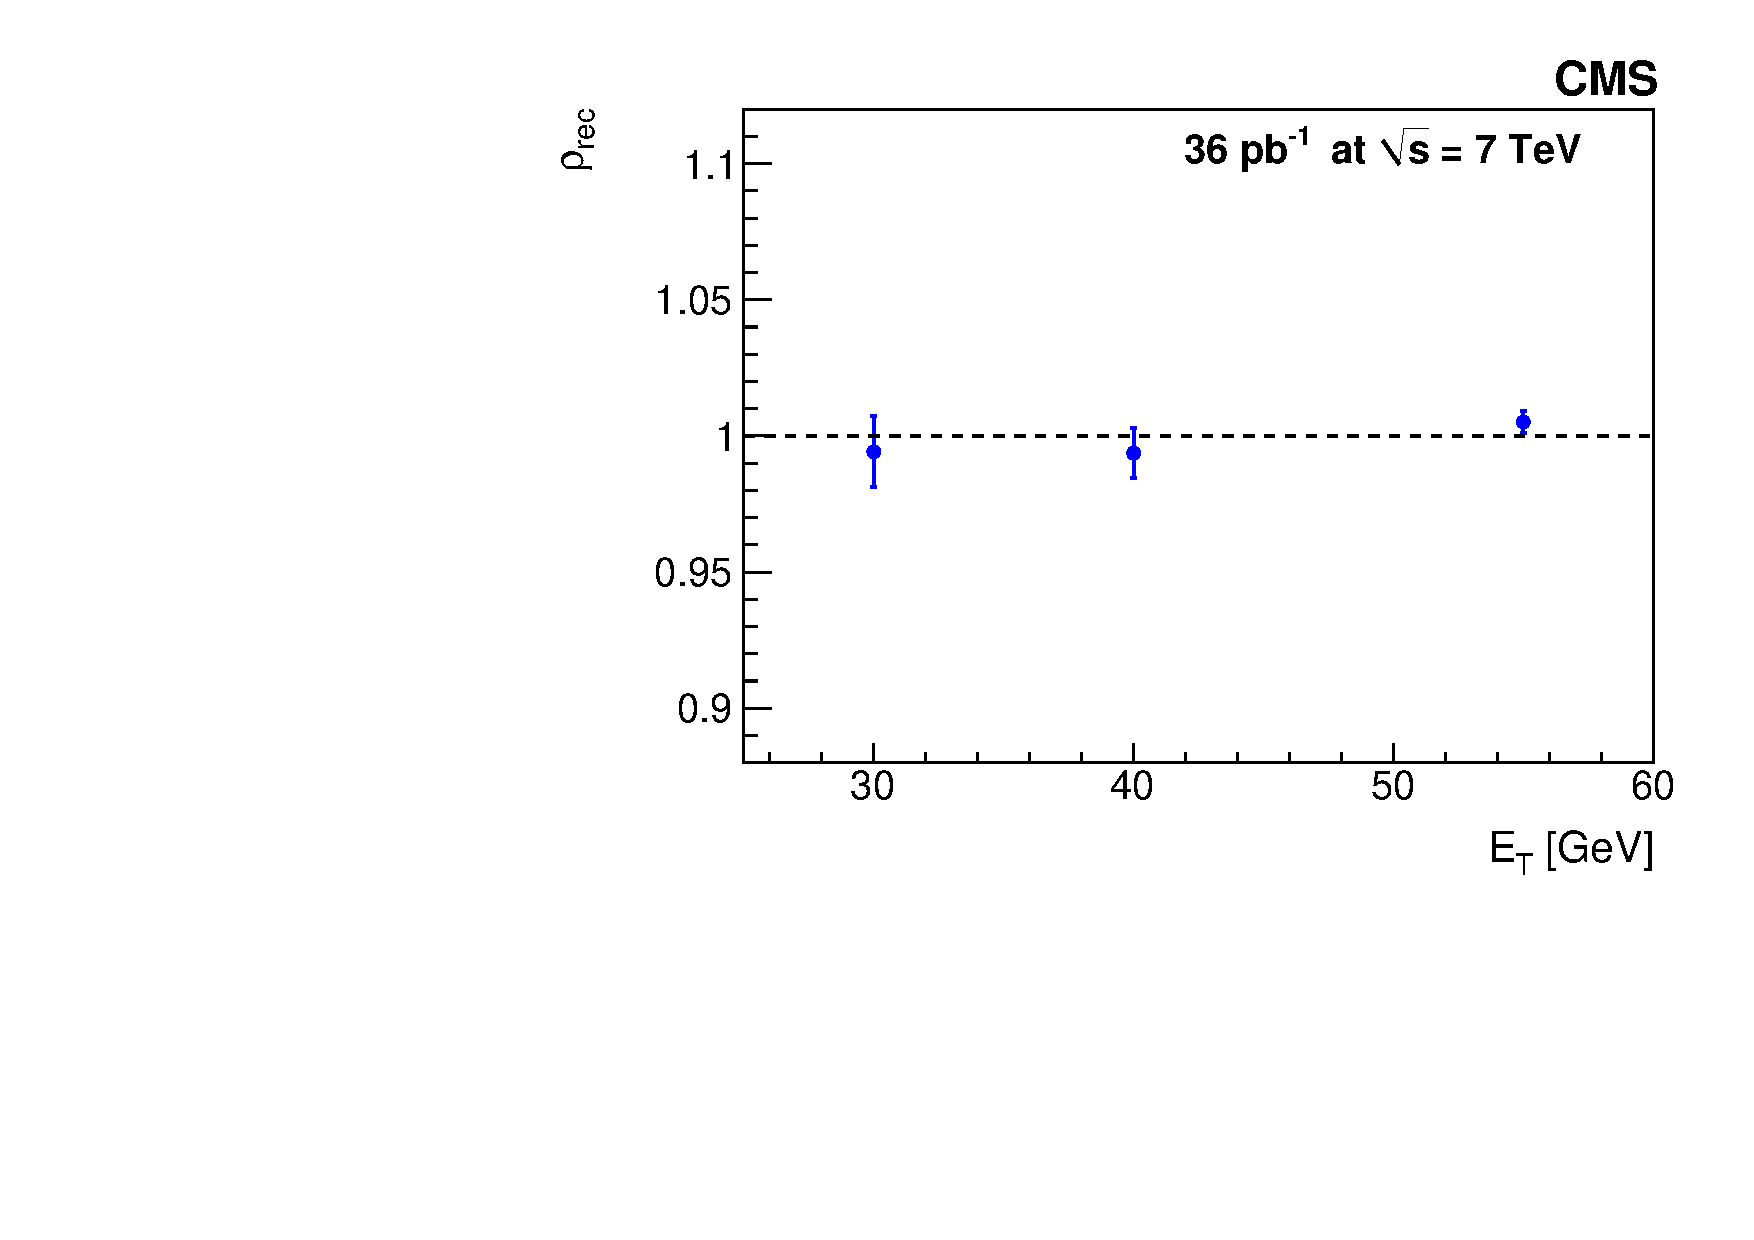
\includegraphics[width=0.48\textwidth]{figs/recoeff_scalept.pdf}
  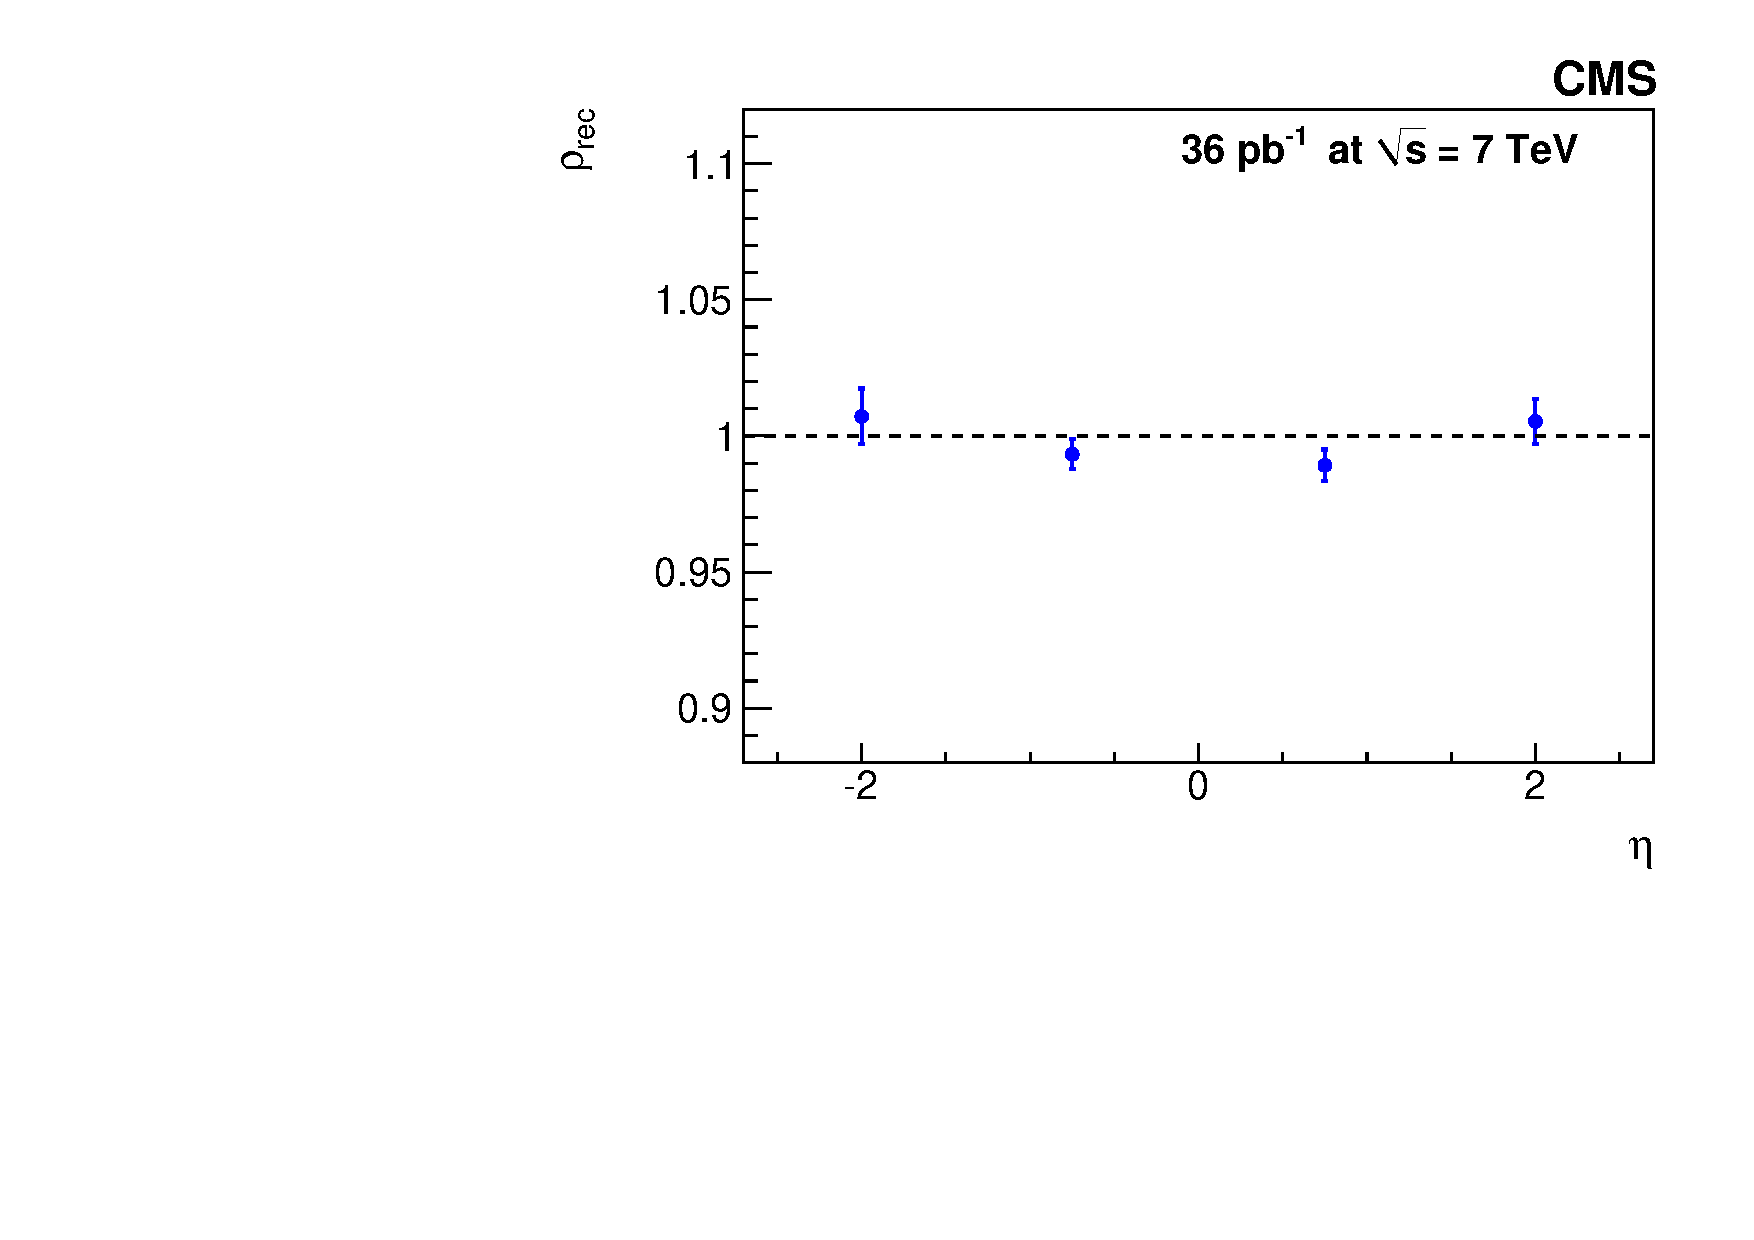
\includegraphics[width=0.48\textwidth]{figs/recoeff_scaleeta.pdf}
% \end{minipage}
% \begin{minipage}[WP80]{0.64\textwidth}
  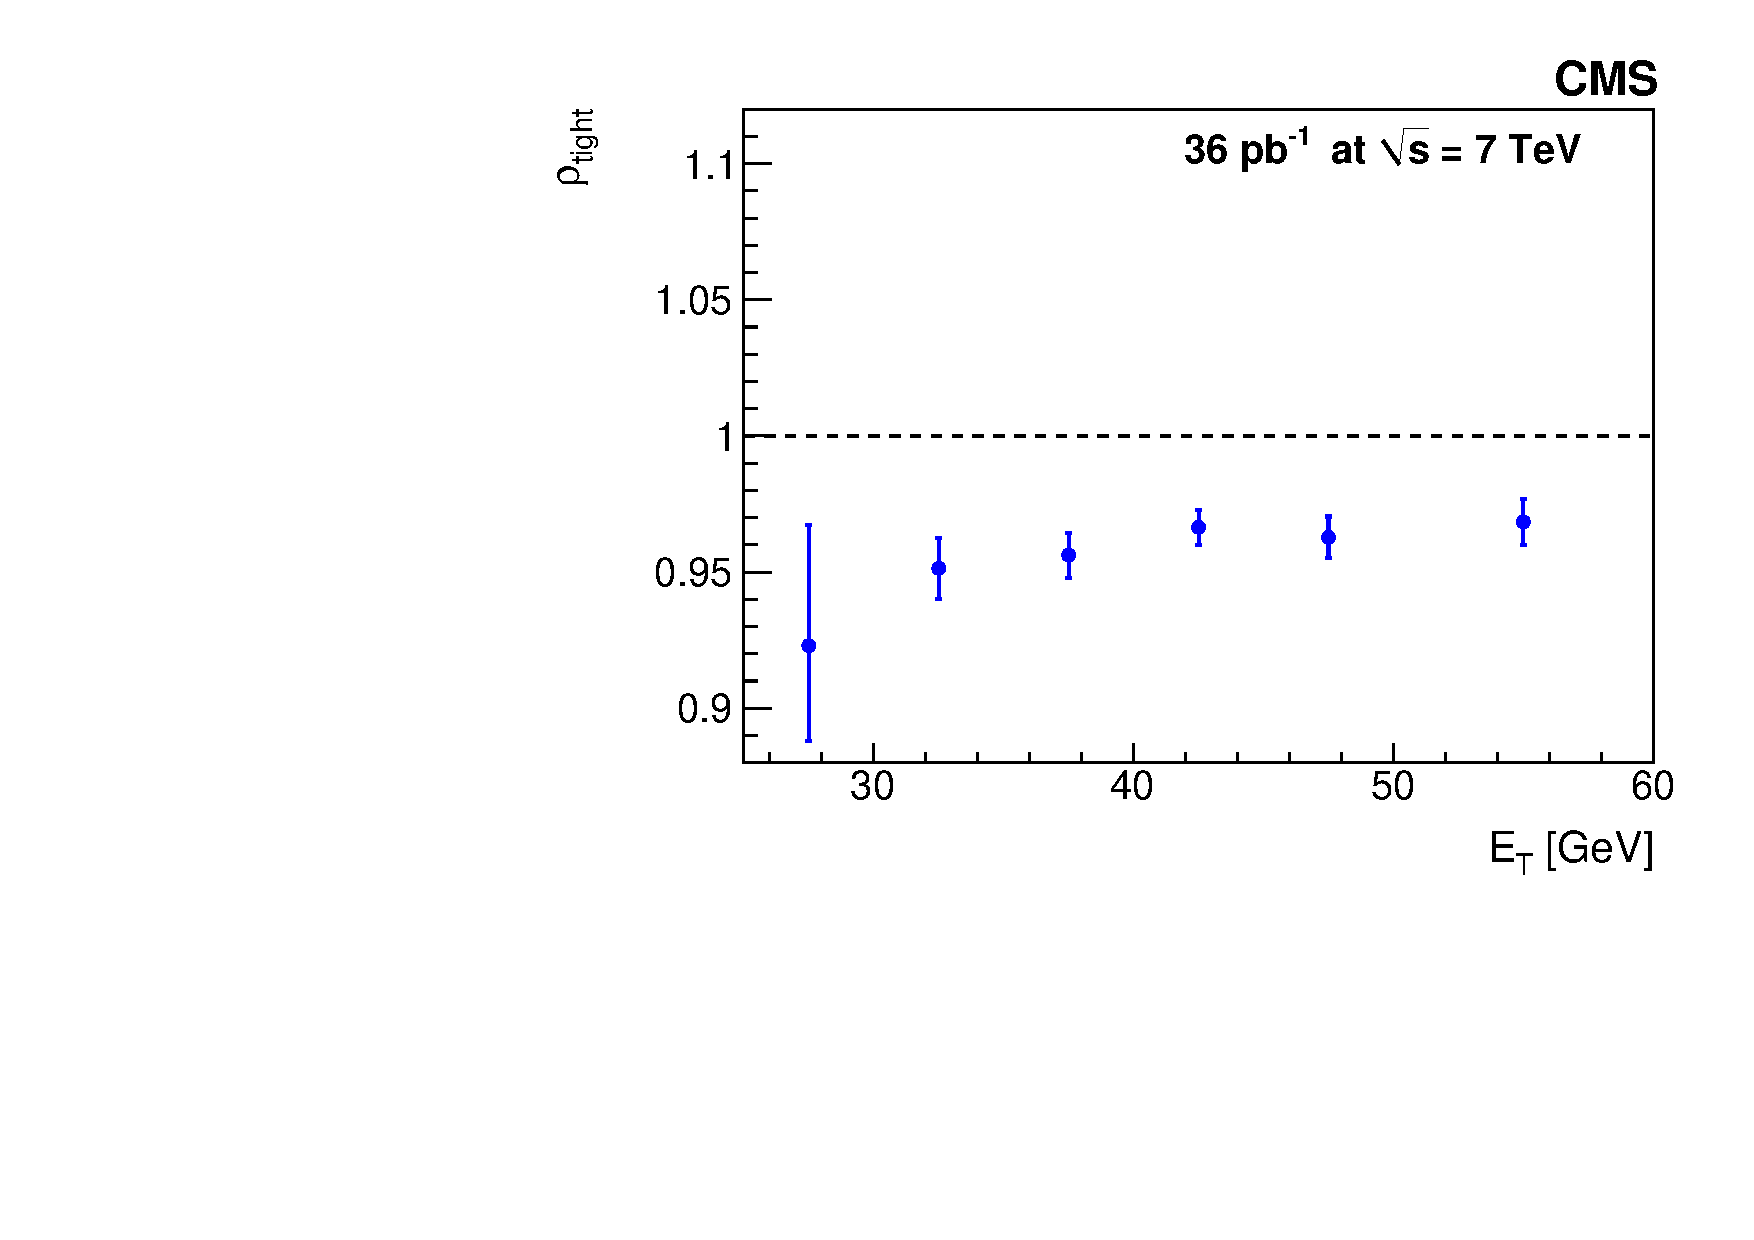
\includegraphics[width=0.48\textwidth]{figs/eleideff_scalept.pdf}
  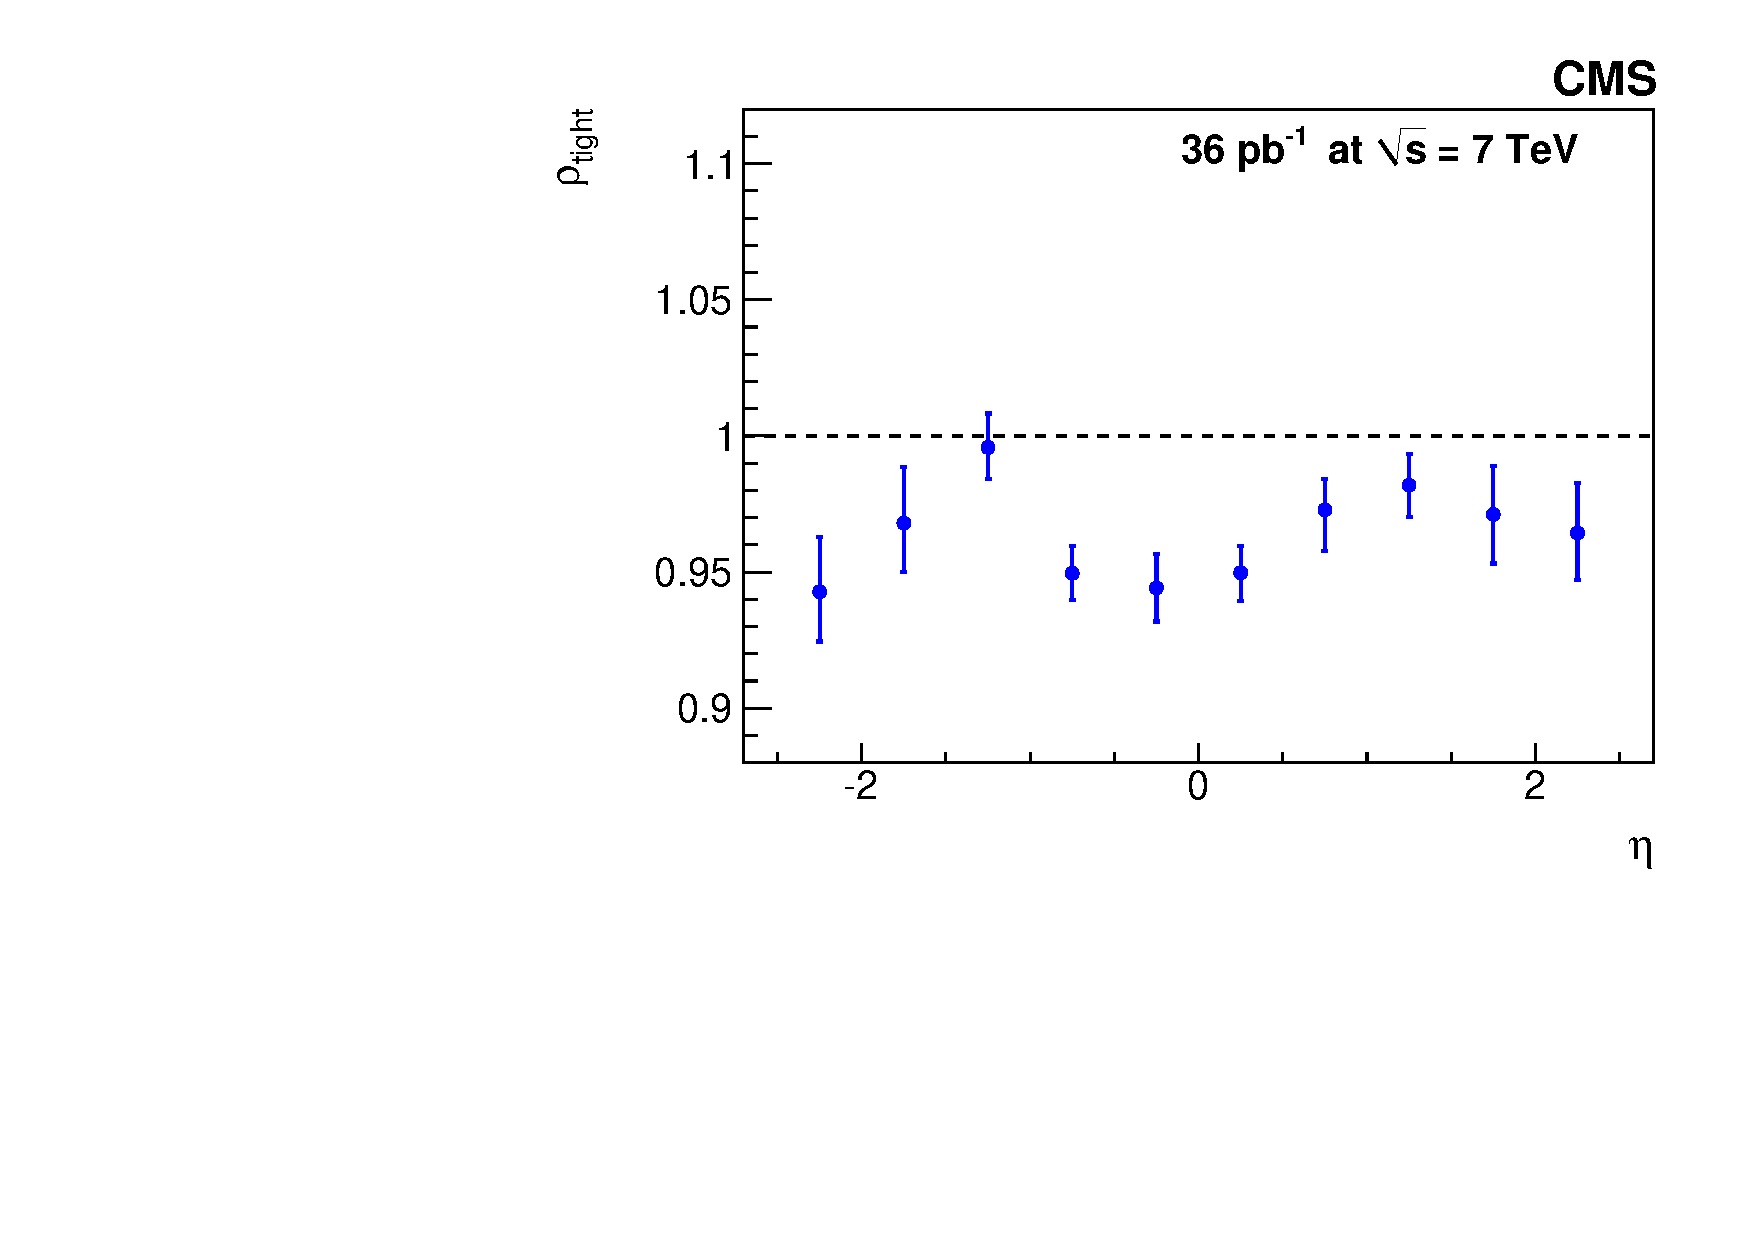
\includegraphics[width=0.48\textwidth]{figs/eleideff_scaleeta.pdf}
% \end{minipage}
% \begin{minipage}[W80toTrigger]{0.64\textwidth}
  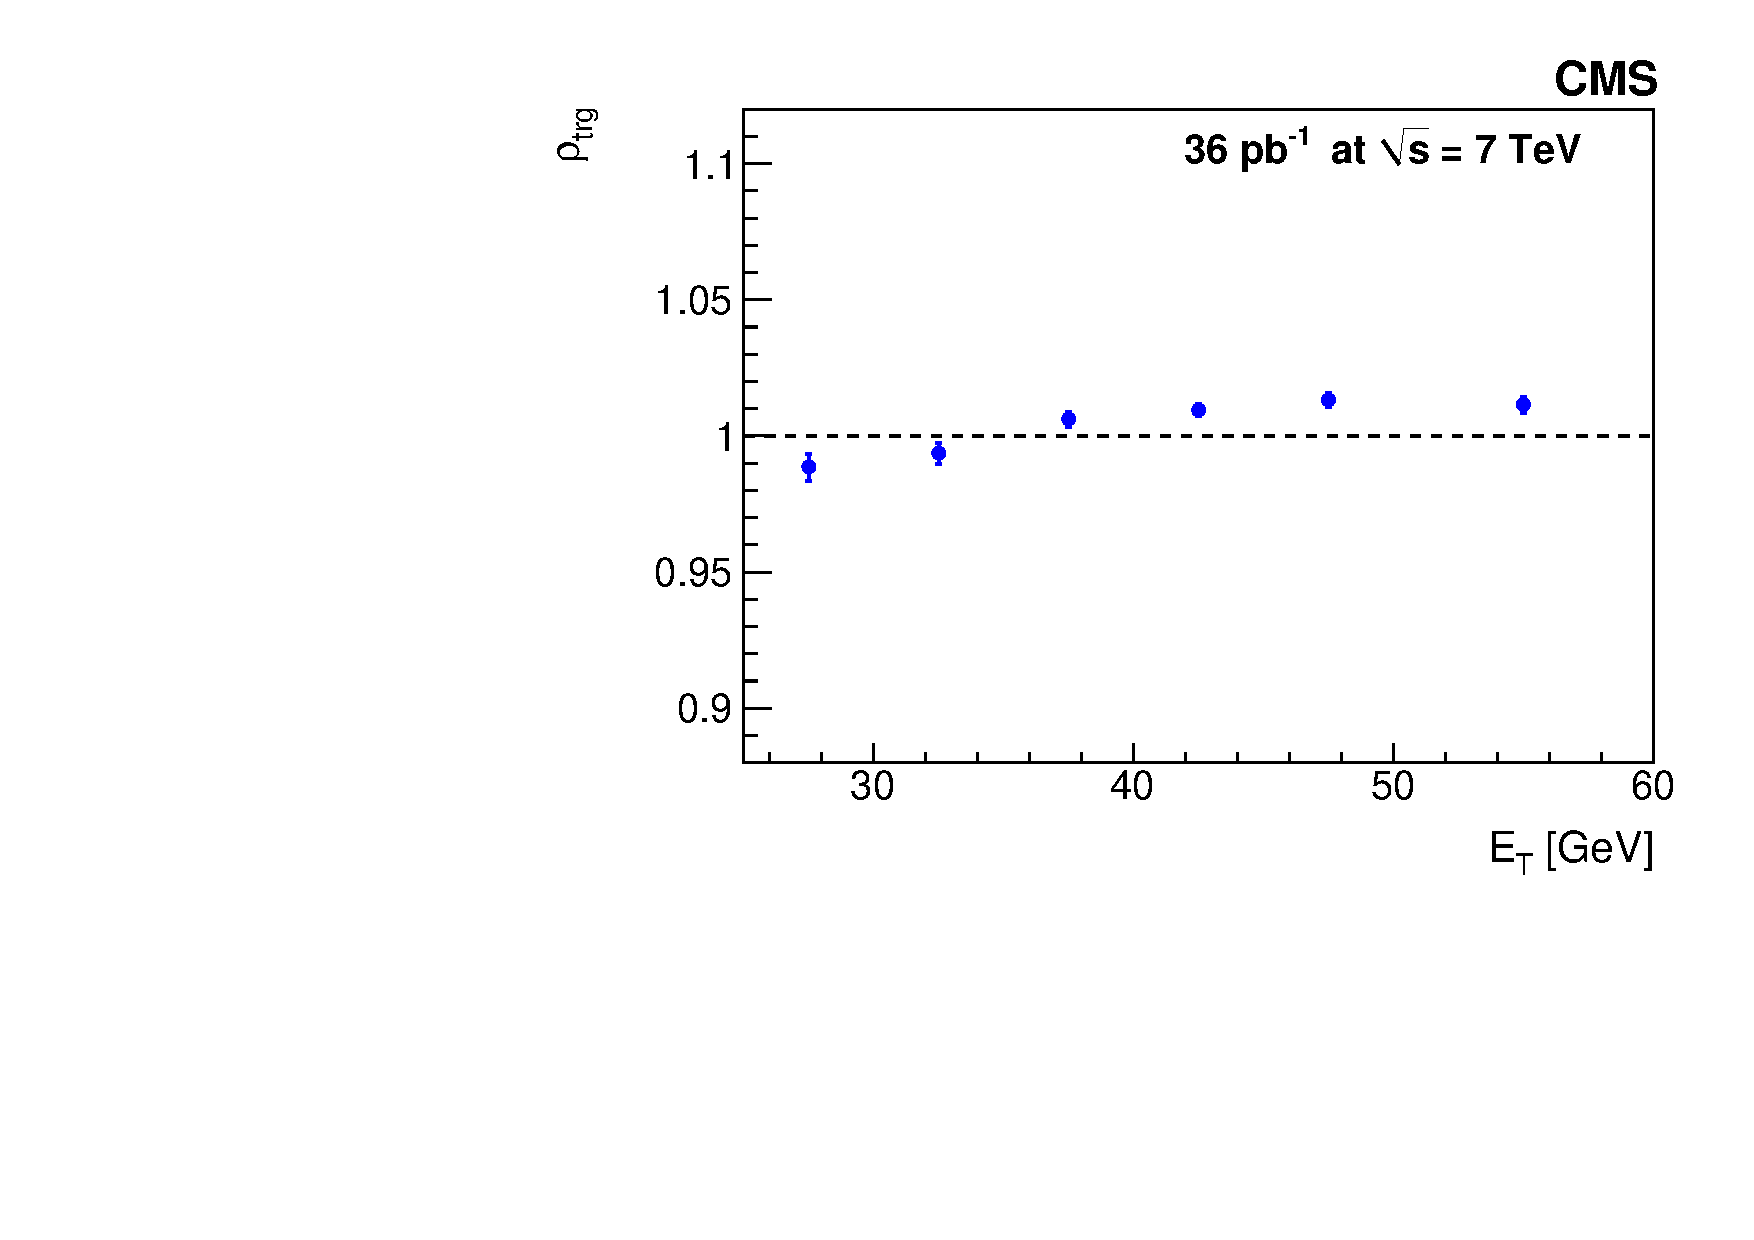
\includegraphics[width=0.48\textwidth]{figs/trigeff_scalept.pdf}
  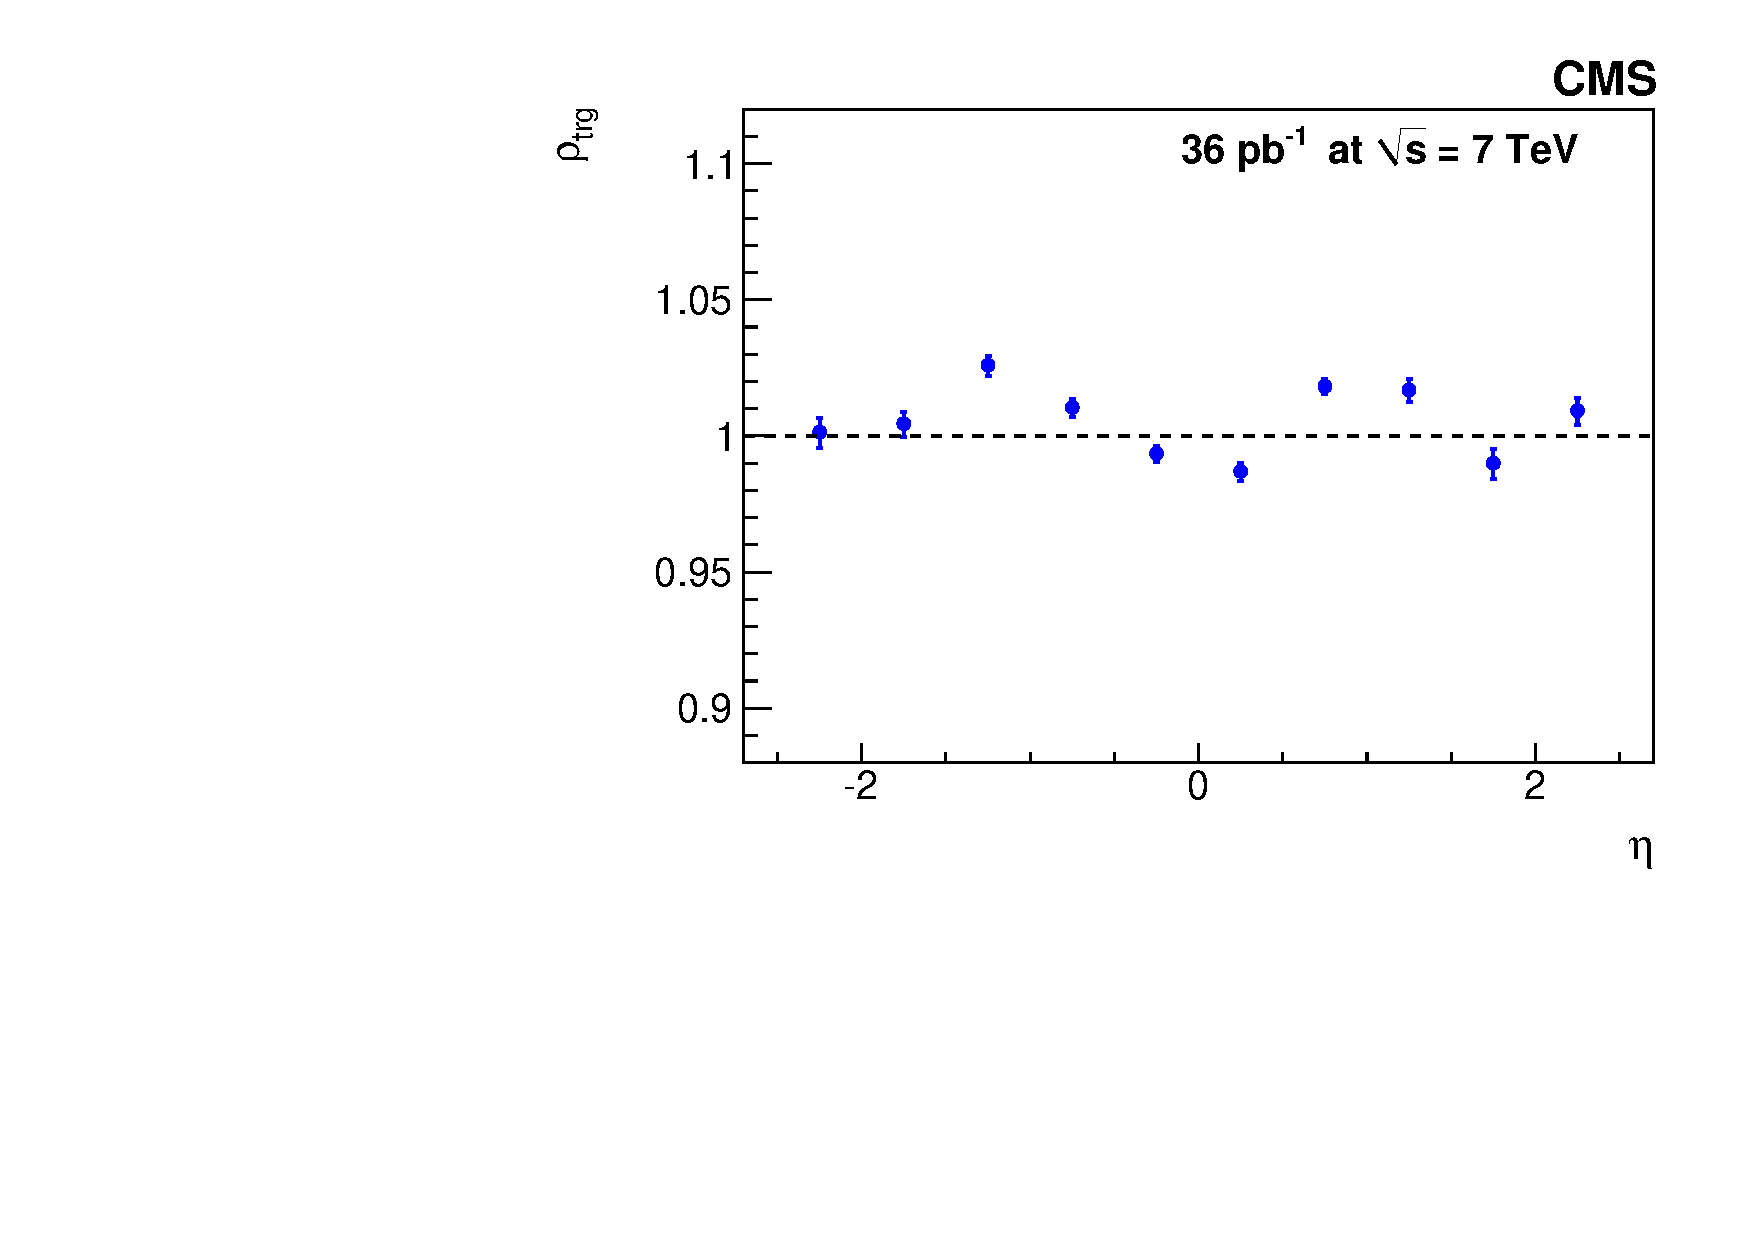
\includegraphics[width=0.48\textwidth]{figs/trigeff_scaleeta.pdf}
% \end{minipage}
 \end{center}
\caption{Data/simulation \TNP ratios versus electron $\Et$ (left column) and $\eta$ (right column).
The ratios are presented for the reconstruction ($\rho_\mathrm{rec}$, top row), selection 
($\rho_\mathrm{tight}$, middle row), and trigger ($\rho_\mathrm{trg}$, bottom row) efficiencies.
Points with error bars represent the ratio measured in data; dashed lines correspond to a constant ratio of one.
\label{fig:e-TnPratios}}
\end{figure}


The $\Zo$ selection efficiencies for data and simulation are obtained based
on the \TNP efficiencies
listed in Table~\ref{tab:e-eff-summary}  and
the event acceptances given in Table~\ref{tab:WZlaccgen}.
The $\Zo$ efficiencies are first determined after
reconstruction and identification (as products of
single-electron efficiencies).
The event trigger efficiency is computed
as the probability that at least one of the two electrons
satisfies the L1+HLT requirement. 
The overall selection efficiency for the $\Zo$ analysis is
the product of the reconstruction, identification, and trigger 
efficiencies. The simulation efficiency obtained from the {\sc POWHEG} $\Zo$ 
samples, together with the final corrected $\Zo$ selection efficiency 
$\effmc \times \rhoeff$, are shown in Table~\ref{tab:el-Zeff}.
These efficiencies are relative to the $\Zo$ events with both electrons within the ECAL acceptance.
%Similarly to the W case, the PDF uncertainties on the corrected $\Zo$ efficiencies 
%were found to be negligible.
\begin{table}[ht] %
  \begin{center}
  \caption{ Simulation efficiency and the final corrected selection efficiency for the ~$\Zee$ analysis.
The quoted uncertainties are statistical for $\effmc$ and include both statistical and 
systematic uncertainties for the corrected efficiency $\effmc \times \rhoeff$.
 \label{tab:el-Zeff}}
  \begin{tabular}{|l|c|c|}
    \hline
     & $\effmc$ & $\effmc \times \rhoeff$ \\
    \hline\hline
    $\Zee$  & \ZEEEFFMC & \ZEEEFF \\
    \hline
    \end{tabular}
  \end{center}
\end{table}


\par
%For later convenience, we define the quantity $A^{\prime}$, which is 
%the overall selection efficiency in the Monte Carlo simulation, as:
%\begin{equation}
%  A^{\prime} = A \times \epsilon
%            = A^{\textrm{ECAL}} \times \EPS{MC} \ .
%\end{equation}



%\subsection{Muon Efficiencies \label{sec:muonEff}}

The muon reconstruction overall selection efficiency 
is determined by the efficiency to find a track in the inner tracker and in the
muon chambers, to pass the isolation requirements, and the probability 
to pass the L1 trigger and HLT.

Tag-and-Probe method is used to determine muon efficiencies for $\Wmn$ cross section determination,
while for $\Zmm$ muon efficiencies are determined simultaneously with the Z yield using a simultaneous
fit technique that is described in Section~\ref{sec:Zmumu}. 
%Tag-and-Probe method uses a clean sample of $\Zmm$ candidates selected from the 36~pb$^{-1}$ available data
%on which about 22000 triggered muon {\em tags} are selected.
%$\Zmm$ events have muon kinematics very similar to those used in the $\Wo$ analysis.
%The possible presence of background processes in the selected event sample has been also taken into account.

%, making use of the 2 million events
%The efficiency ratio 
%$\rho_\mu = {\epsilon_{\mathrm{data}}}/{\epsilon_{\mathrm{MC}}}$ 
%has been calculated in order to be applied to the  
%W cross-section determination. 
The efficiencies have been studied as a function of muon pseudorapidity and transverse momentum, 
to reproduce better the real detector performance. 
The promediated efficiencies are estimated to be
$\epsilon_{\mathrm{data}} = 0.8548 \pm 0.0025\, \mathrm{(stat)} \pm  0.024\, \mathrm{(syst)}$ and
$\epsilon_{\mathrm{MC}} = 0.8989  \pm   0.0004\, \mathrm{(stat)}$ in data and Monte Carlo respectively,
hence a correction factor of $\rho_\mu= 0.9509 \pm  0.0028 \mathrm{(stat)} \pm  0.024\, \mathrm{(syst)}$
has been appled to the data.
The quoted systematic errors take into account the fit parameter uncertainties stemming 
from the correction of the background.

Single-muon efficiencies have also been determined separating in positive or negative charged muons, 
obtaining the following correction factors: $\rho_\mu^+ = 0.957 \pm 0.004\,\mathrm{(stat)} \pm 0.024\,\mathrm{(syst)}$,
$\rho_\mu^- = 0.945 \pm 0.004\,\mathrm{(stat)} \pm 0.024\,\mathrm{(syst)}$.

A small fraction (0.5\%) of muon events is lost because of Level-1 trigger pre-firing
due to the wrong assignment to the muon bunch crossing number, due to imperfect timing. 
Cross sections in muon channels have been corrected by this effect and
the uncertainty on the correction factor has been taken as systematic uncertainty.

\section{Event Selection\label{sec:evtSel}}
\par
We used the data-taking periods from 2010 LHC operations 
passing the standard CMS quality criteria, which allow no anomalous or
faulty behavior for the inner tracker, the calorimeters,
and the muon chambers.
\par
Several large samples of simulated events were used to evaluate the signal
and background efficiencies and to validate our analysis techniques.
Samples of electroweak processes with $\Wo$ and $\Zo$ production, both for
signal and background events, were produced with
POWHEG~\cite{Alioli:2008gx, Nason:2004rx, Frixione:2007vw},
interfaced with the PYTHIA~\cite{Sjostrand:2006za} parton-shower generator.
QCD events with muons, electrons, or jets likely to be misidentified
as electrons in the final state were studied with PYTHIA, as were other minor
backgrounds such as $\ttbar$ and certain electroweak processes
($\Wtn$, $\Ztt$, $\Wo\Wo$, $\Wo\Zo$, and $\Zo\Zo$).
We do not consider the diboson channels ($\Wo\Wo$, $\Wo\Zo$, and $\Zo\Zo$)
as part of the $\Wo$ and $\Zo$ signals in order to facilitate the comparison 
of our results to theoretical predictions,
which do not take these contributions into account.
Generated events were processed through the full GEANT4~\cite{GEANT4} detector 
simulation, trigger emulation, and event reconstruction chain.

\subsection{$\Wo$ boson selection}

\par
The $\Wo$ events are characterized by a prompt, energetic, and
isolated lepton, and significant missing energy.
The main backgrounds are QCD multijet events and Drell-Yan (DY)
events in which one lepton fails the selection.  The QCD background is
reduced by requiring the lepton to be isolated; the remaining
events do not have large $\MET$ and can be distinguished from
signal events on a statistical basis.  The DY background
is suppressed by rejecting events with a second lepton candidate.

To measure the signal yields, we choose to fit the $\MET$
distribution for both the electron and muon channels.
According to the simulation, $\Wtn$ background contribution is small,
while backgrounds from $\Ztt$, $\ttbar$, and diboson production
are negligible in both electron and muon channels.

\subsection{$\Wen$ signal extraction\label{sec:Wen}}

The $\Wen$ candidate events are required to have one identified electron
with an ECAL cluster of $\et > 25\GeV$ in the ECAL fiducial volume.
If a second electron candidate
satisfying looser criteria and with $\et > 20\GeV$ is present in
the event, the event is rejected.
%The fraction of signal events selected in the simulation is
%$\APRIM{\Wo} = \WEIAPRIM$, with  $\APRIM{\Wop}=\WEPAPRIM$ and
%$\APRIM{\Wom}=\WEMAPRIM$.
The number of events selected in the data
is $\WEISAMPLE$, with $\WEPSAMPLE$ positive and $\WEMSAMPLE$
negative electrons.
\par
The $\Wen$ signal is extracted from an unbinned maximum likelihood
fit of the observed $\MET$ distribution to the sum of signal and
background shapes.
The QCD background shape, which accounts
for both QCD multijet production and direct-photon
production with the photon converting in the detector,
can be modeled by a modified Rayleigh distribution,
$$f(\MET) = \MET \times \exp{\left(-\frac{\MET^2}{2(\sigma_0+\sigma_1\MET)^2}\right)}.$$
This function can be understood as describing fluctuations of the
missing transverse momentum vector around zero due to measurement errors;
%the resolution term, $\sigma_0+\sigma_1 \MET$, increases
%with $\MET$ to account for tails in the $\MET$ measurement.  
%This function describes well the QCD background shape in the simulation, over the full
%range of $\MET$, as well as $\MET$ distributions from signal-free samples obtained by 
%inverting the identification or isolation criteria.
The fit to the anti-selected sample shown on
Fig.~\ref{fig:e-inverted} illustrates the quality of the description
of the background shape by our parameterized function,
including in the region of the signal, at high \MET.
\begin{figure}[b]
\begin{center}
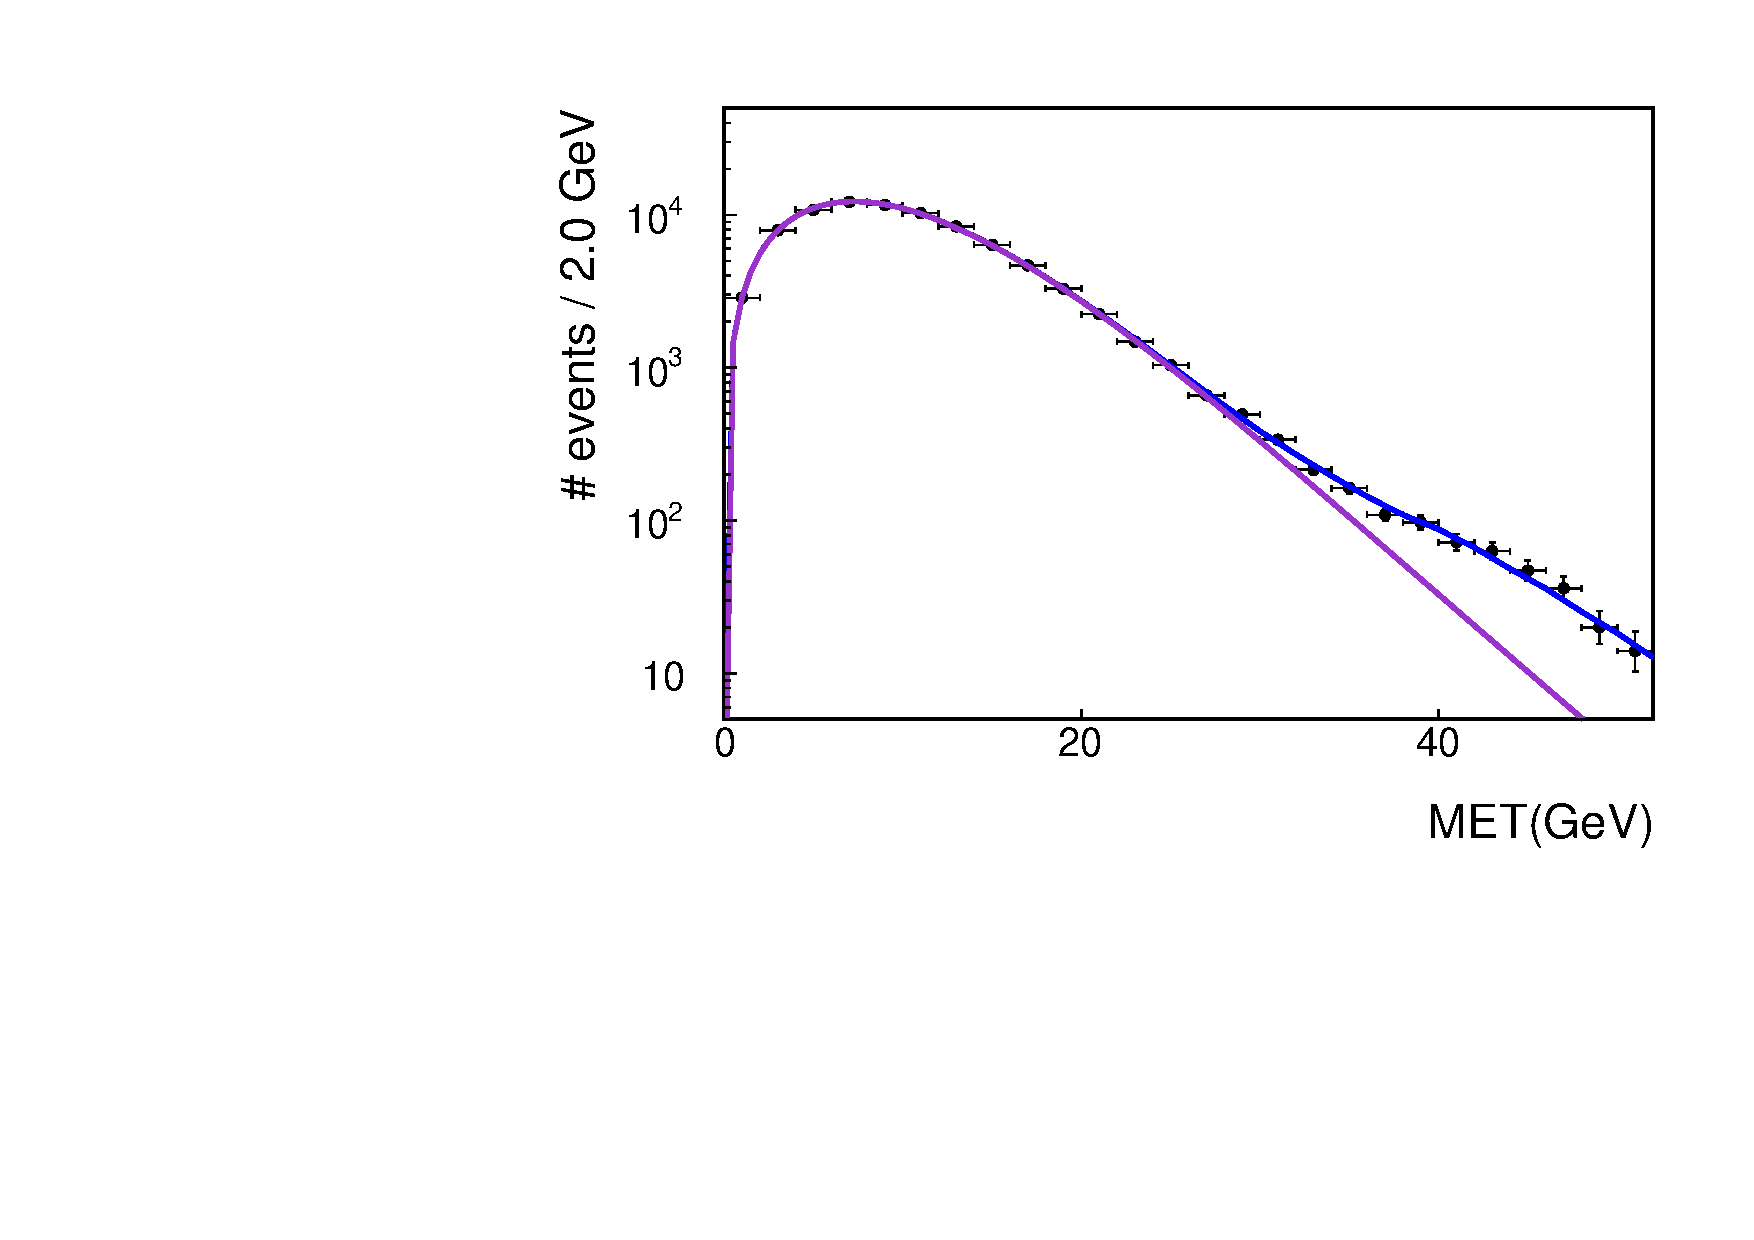
\includegraphics[width=0.50\textwidth]{figs/fixedMCyield_normal_model.pdf}
\caption{Fit to the anti-selected background sample (we invert cuts on the track-match
variables while maintaining the usual \ET and ECAL-iso selections).
}\label{fig:e-inverted}
\end{center}
\end{figure}


The signal distributions are derived from simulation,
separately for $\Wp$ and $\Wm$, and receive
an event-by-event correction in bins of the $\Wo$ transverse momentum,
determined from a study of the hadronic recoil
distributions of $\Zee$ events in the data.%~\cite{CMS-PAS-JME-10-005}.
In fig.~\ref{fig:Recoil} the left-hand side plot demonstrates the effect of the recoil
corrections on the MET shape for the electron channel while the right-hand side plot
shows the uncertainty from the recoil method propagated to the corrected W MET shape.


%%%%%%%%%%%%%%%%%%%%%%%%%
\begin{figure}
\begin{center}
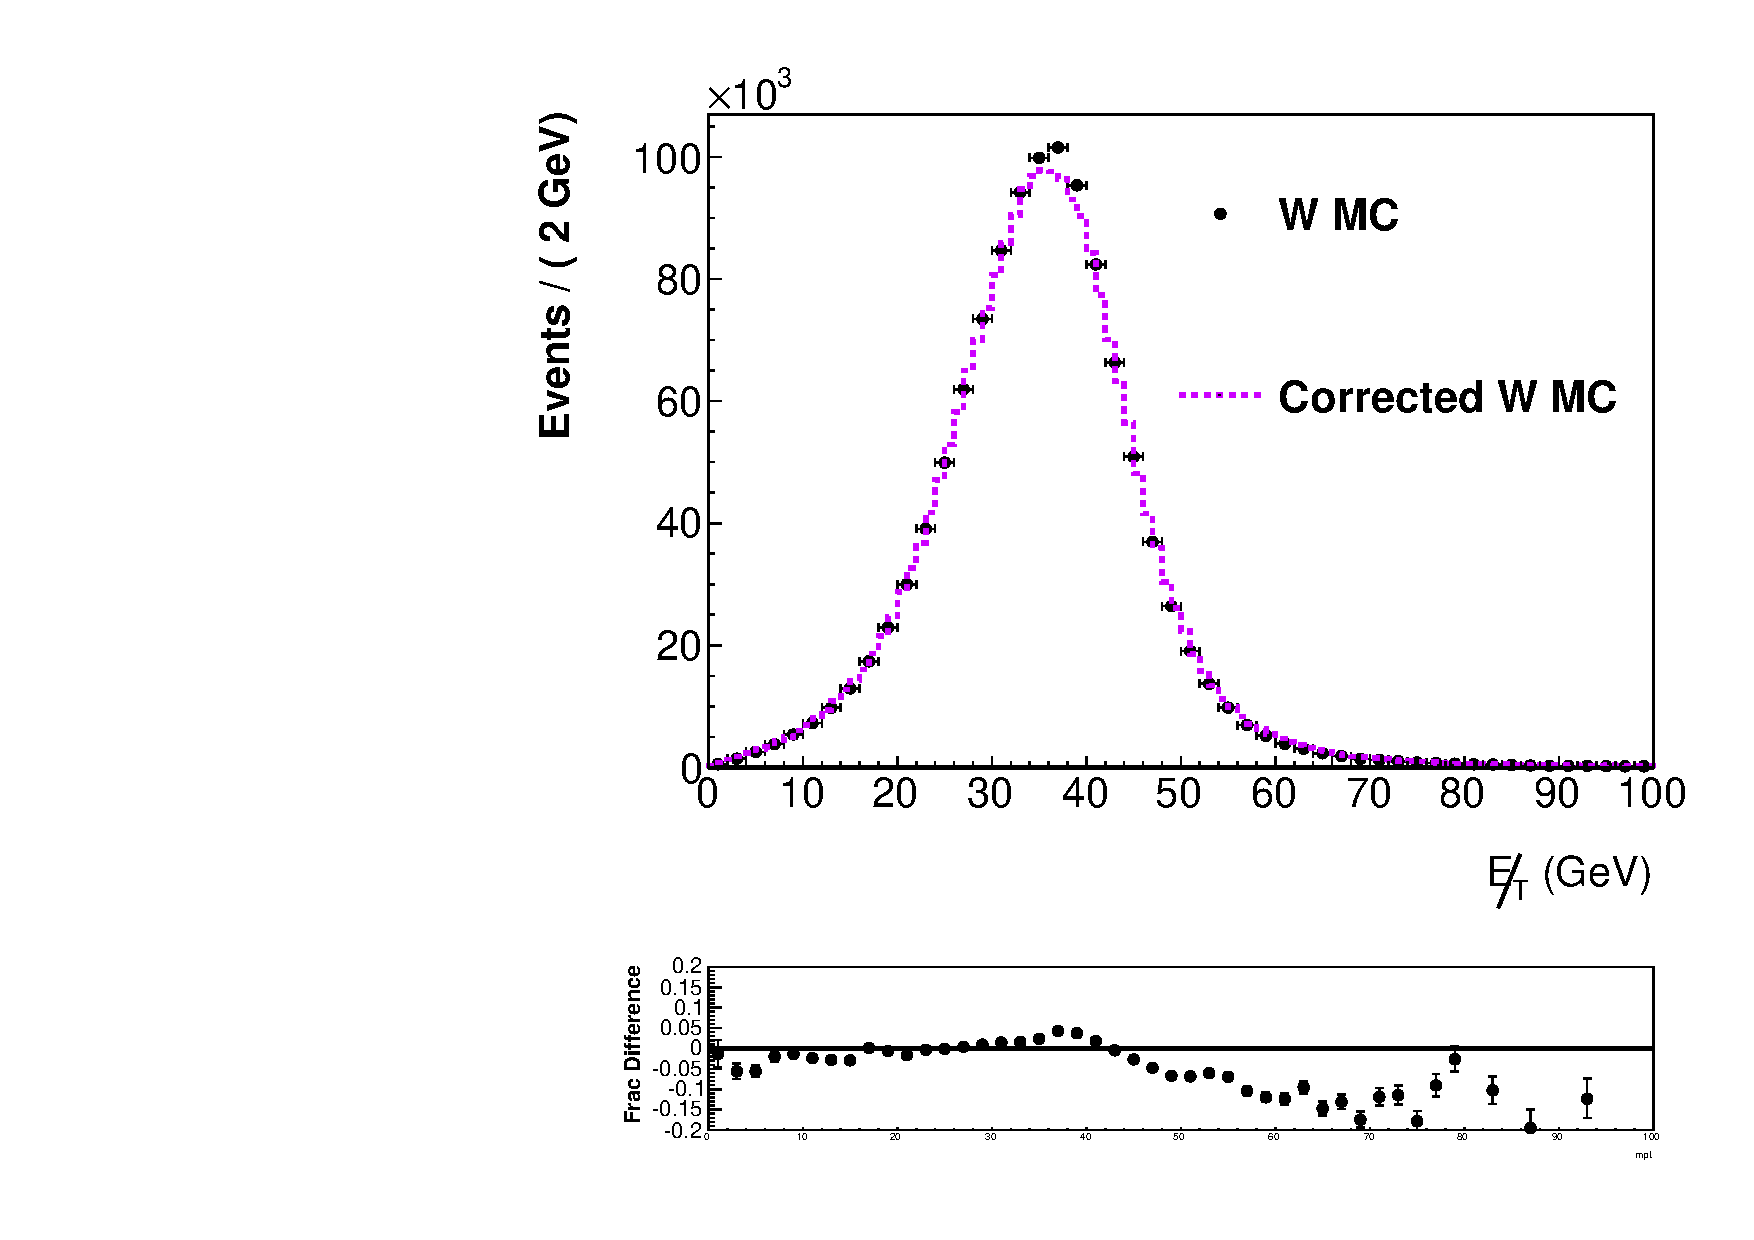
\includegraphics[width=0.48\textwidth]{figs/beforeANDafter.pdf}
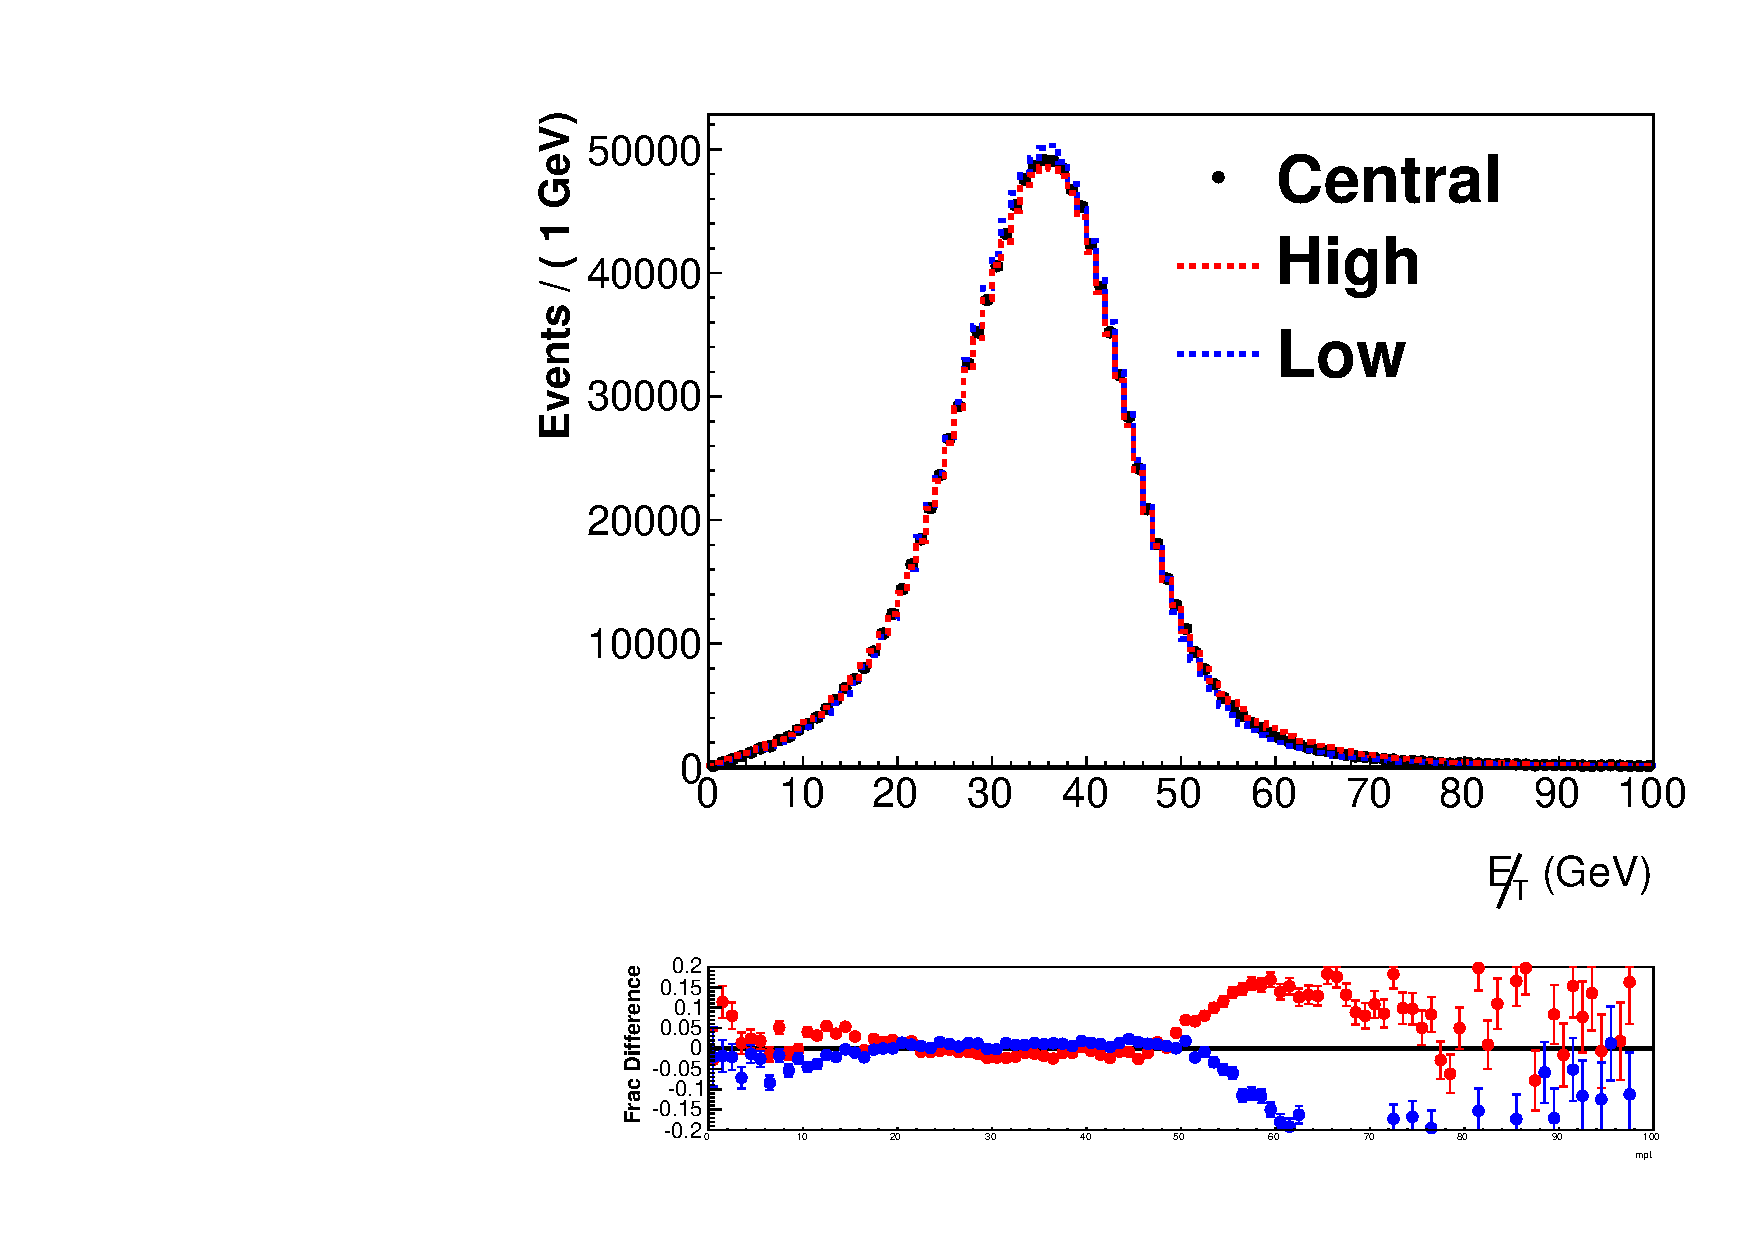
\includegraphics[width=0.48\textwidth]{figs/upANDdown.pdf}
\caption{ \label{fig:Recoil}
Demonstration of the recoil corrections on the $\Wen$ $\MET$ shape (left)
and uncertainties from the recoil method propagated to the corrected
$\Wen$ $\MET$ shape (right).
}
\end{center}
\end{figure}
%%%%%%%%%%%%%%%%%%%%%%%%%


%In fits to the $\MET$ distributions, the free parameters
%are the $\Wo$ signal yield, the QCD background yield, and
%the shape parameters $\sigma_0$ and $\sigma_1$.

We extract the inclusive yield $\NSIG{\Wo}$ from a fit where
the expected ratio for $\XVL{\sigma}{(\Wp)}/\XVL{\sigma}{(\Wm)}$
is assumed.
It has been  checked that the result was insensitive to this assumption.
Figure~\ref{fig:Wenu}~(a) shows the $\MET$ distribution of
the inclusive $\Wen$ sample
and the results of the likelihood fit.
%the fit function describes the
%data well, with a $p$-value of $\WEIKSPCOR$ for the Kolmogorov-Smirnov test.
The inclusive yield is $\NSIG{\Wo} = \WEIYIELD$ events.

%%%%%%%%%%%%%%%%%%%%%%%%%
\begin{figure}[t]
\begin{center}
         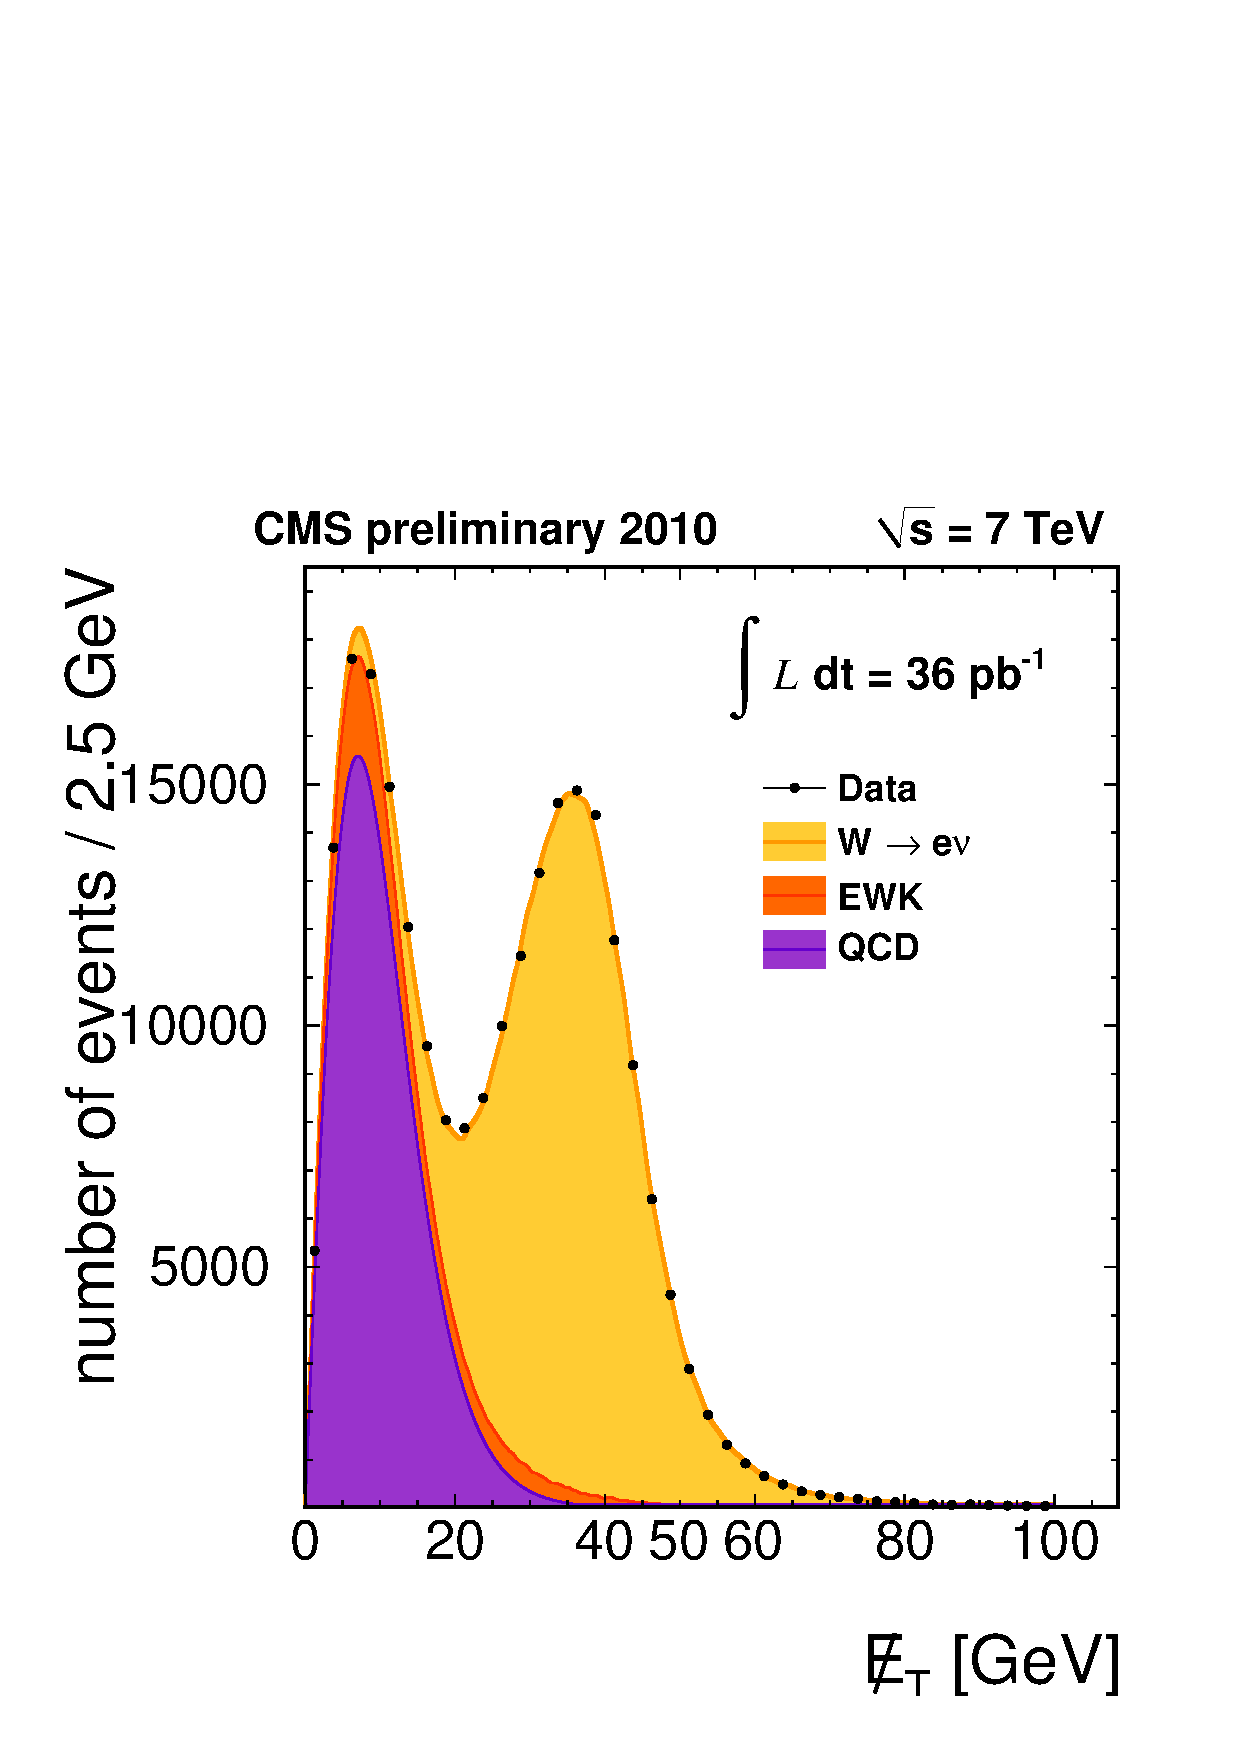
\includegraphics[width=.45\textwidth]{figs/w_inc_36pb.pdf}
        \hspace{.05in}
         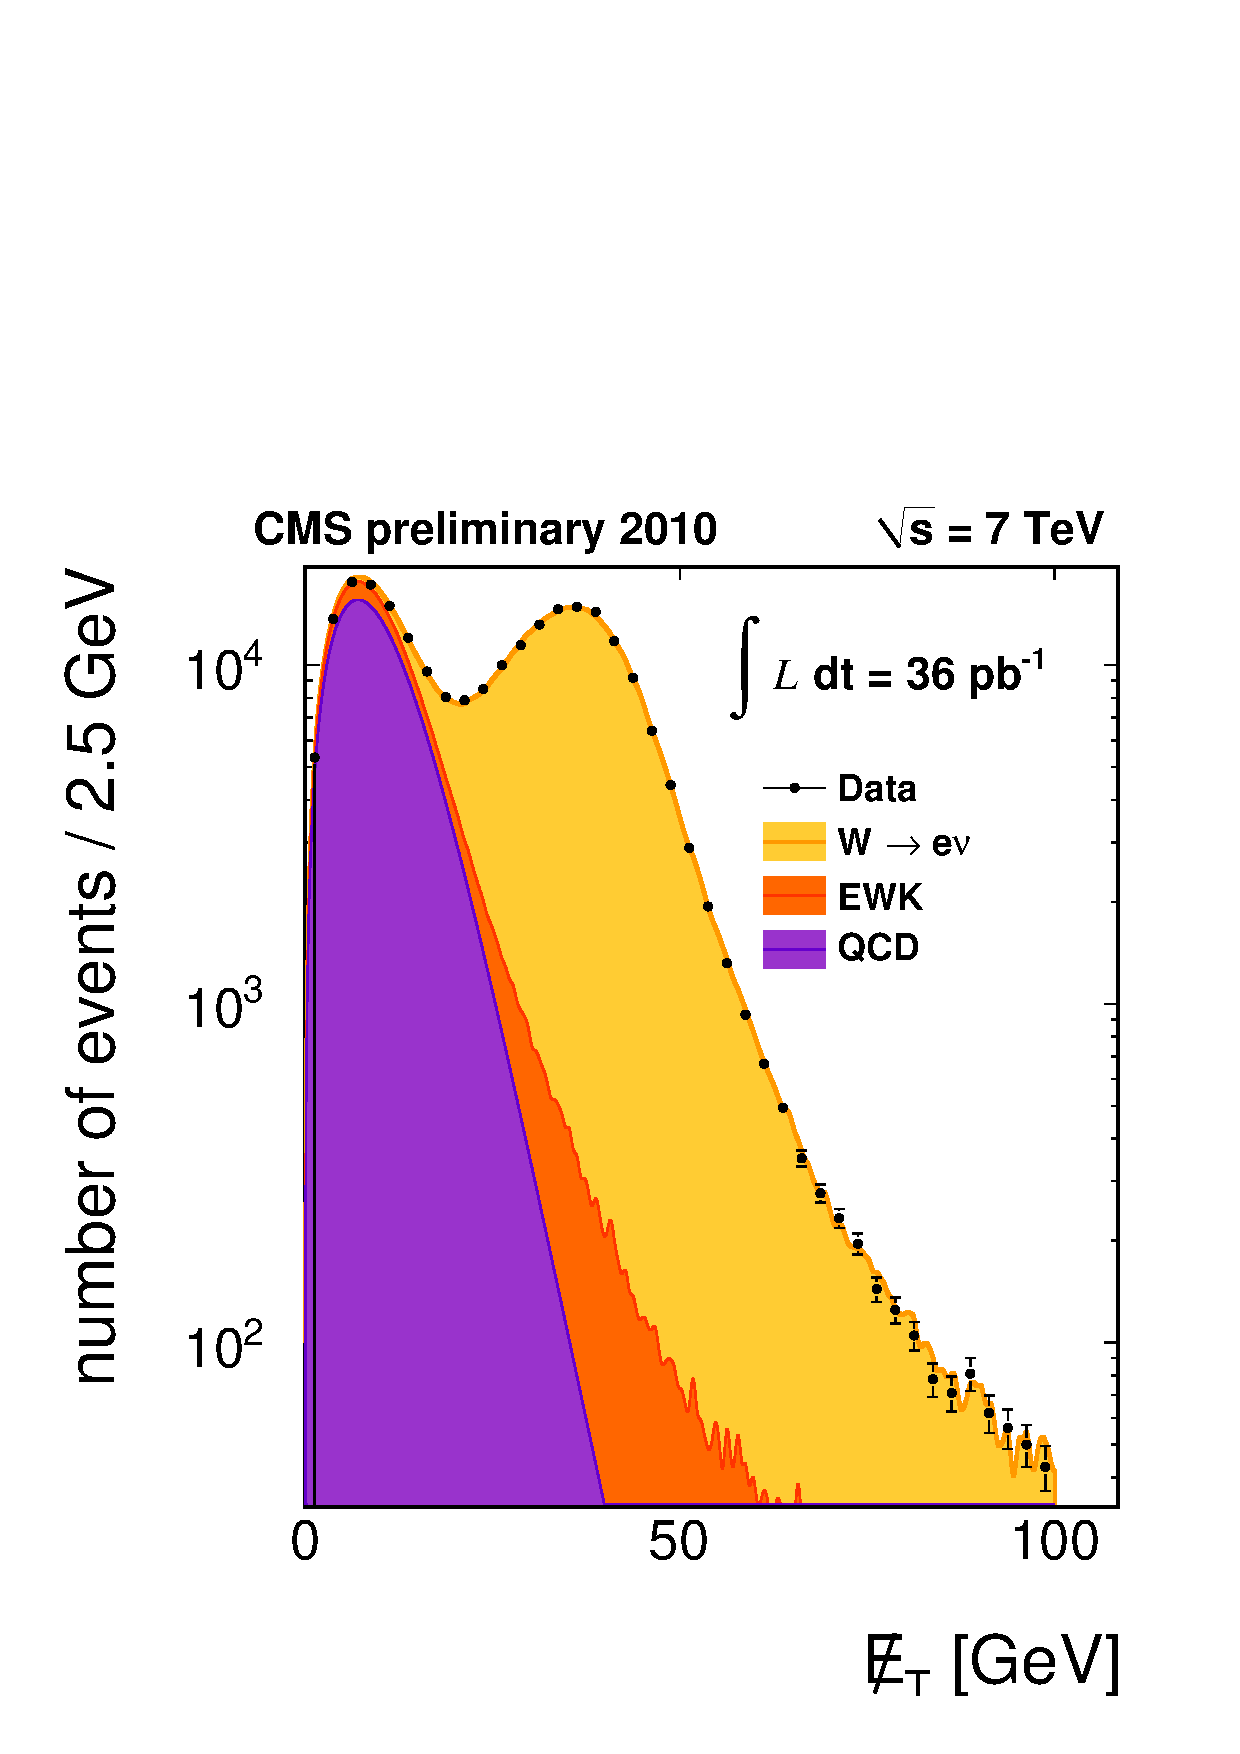
\includegraphics[width=.45\textwidth]{figs/w_inc_36pb_log.pdf}
        \hspace{.05in}
       \caption{The $\MET$ distributions for the $\Wen$ candidates:~(a)
linear scale;~(b)~log-scale.  The points represent
the data.  Superimposed are the results of the maximum likelihood fits for
signal plus backgrounds, in yellow; all backgrounds, in orange;
QCD backgrounds, in violet.
\label{fig:Wenu} }
\end{center}
\end{figure}
%%%%%%%%%%%%%%%%%%%%%%%%%


The signals for the $\Wpen$ and $\Wmen$ channels are
extracted from a simultaneous fit to the individual $\MET$
distributions, in which the QCD background  shape parameters $\sigma_0$ and
$\sigma_1$ are constrained to be the same for both samples.
The yields are $\WEPYIELD$ for $\Wpen$ and $\WEMYIELD$
for $\Wmen$, with a negligible correlation.
%Because the two fits are independent,
%the relation $\NSIG{\Wo} = \NSIG{\Wop} + \NSIG{\Wom}$ is not exactly satisfied,
%but holds to within 0.2\%.

Two additional signal extraction techniques were explored. 

In the first approach the QCD \MET template is extracted directly from the data using a
control sample obtained by inverting a subset of the cuts used to select the
signal. In this way, the shape of the template is fixed from the data, and
only the normalization is allowed to float in the fit. 
%The advantage of this approach
%is that detector effects such as anomalous signals in the calorimeters, or
%dead ECAL towers, are automatically reproduced in the QCD template, since these
%effects are not affected by the cut inversion used to define the control sample.
Possible differences in shape between the selected and anti-selected \MET
distributions has been found to be due to a combination of two effects,
and can be eliminated by applying corrections.  In the
Particle Flow algorithm, electron candidates contribute differently to
\MET depending on the output of a multivariate analysis (MVA) used to identify
electrons.  A correction is applied to account for the fact that the
distribution of the MVA output is very different in the signal and
control samples, resulting in a bias to the \MET shape.  The second
correction accounts for the effect of a small observed correlation between
one of the inverted variables and \MET.  The correction is derived by performing linear
fits, separately for the ECAL barrel and endcaps, to profile histograms of
the mean value of \MET in slices of the inverted variable.


The results of inclusive fits for \MET and $M_T$ using the fixed shape QCD
template are shown in Figure~\ref{fig:resultAll}.

\begin{figure}[htb]
  \begin{center}
    \includegraphics*[width=0.9\textwidth]{figs/resultsAll.pdf}
    \caption{Result of fixed shape template fits for \MET (left) and $M_T$
(right) for all W candidates.  The bottom plots show the ratio of the data to
the sum of the fitted templates.}
    \label{fig:resultAll}
  \end{center}
\end{figure}

%By applying the method we obtain the following yields:
% 134894 $\pm$ 384 for the inclusive sample, xx $\pm$ xx for $\Wpen$ sample and
% xx $\pm$ xx for $\Wmen$ sample. Those yields are in good agreement with the
% parametrized fits method.

By applying the method we obtain a yield of 134894 $\pm$ 384 (stat) for the inclusive sample. 
The ratio of the inclusive yields between this method and the parameterized QCD shape is
0.989 $\pm$ 0.005 considering only the uncorrelated systematics between the two methods. 

In the second approach the data are divided into 5 categories defined by cuts 
on $\MET$ and relative tracker isolation of the electron candidate.
The ABCD region in this method roughly maps onto the AB region of the older approach, 
with the E box mapping onto the CD region. This particular arrangement is chosen to minimize 
the sensitivity to uncertainties on the background model. A system of equations is constructed 
relating the number of observed data events in each of the four regions to the number of 
background and signal events, with a number of parameters to be determined from auxilliary 
measurements or simulations. By applying the method we obtain the following yields:
135858 $\pm$ 496 (stat) for the inclusive sample, 81407 $\pm$ 384 (stat) for $\Wpen$ sample and
54319 $\pm$ 315 (stat) for $\Wmen$ sample, with negligible correlation.
The ratio of the inclusive yields between this method and the parameterized QCD shape is
0.997 $\pm$ 0.007 considering only the uncorrelated systematics between the two methods. 

The EWK backgrouds consist mainly of $\Zee+\Ztt$ (7.6$\%$), $\Wtn$ (3.0$\%$), 
di-bosons (0.14$\%$) and $\ttbar$ (0.44$\%$).


\subsection{\texorpdfstring{Modeling of the QCD Background and $\Wmn$ Signal Yield}{Modeling of the QCD Background the W->mu nu Signal Yield}}
\label{sec:Wmunu}

The $\Wmn$ analysis is performed using fixed distributions for the $\MET$ shapes
obtained from data for the QCD background component and from simulations,
after applying proper corrections, for the signal and the remaining background components.

Different approaches to signal extraction are considered for $\Wmn$, as for $\Wen$.
The alternative methods do not demonstrate better performance than the use of fixed shapes
in the W signal fit. Given the lower backgrounds in the muon channel with respect to the
electron channel, the alternative strategies are not pursued at the same level of detail
as in the electron case.

The $\MET$ shape of the QCD background component is obtained from a high-purity QCD sample
of events that pass the signal selection, except that the isolation requirement
is inverted and set to $\IRelComb > 0.2$ (Fig.~\ref{figure:Wmunu_iso}).

Simulation studies indicate that this distribution does not accurately
reproduce the $\MET$ shape when muon isolation is required.
This is shown in Fig.~\ref{figure:Wmunu_QCD} (left),
where the solid line represents the shape for events with an isolated muon and the dashed line
the shape obtained by inverting the isolation requirement. %They are very distinct.

A positive correlation between the isolation variable $\IRelComb$ and $\MET$ is shown
in Fig.~\ref{figure:Wmunu_QCD} (right, red open circles). This behavior can be
parameterized in terms of a linear function
$\MET\propto (1+\alpha\,\IRelComb)$, as shown in the same figure.
A compensation for the correlation is subsequently made
by applying a correction of the kind of $\MET^\prime = \MET/(1+\alpha\,\IRelComb)$ to
the events selected by inverting the isolation requirement and a new corrected shape is obtained.
The agreement of this new shape (black points in Fig.~\ref{figure:Wmunu_QCD}, left)
with the prediction from events with an isolated muon is considerably improved.
It is also observed that a maximal variation in the correction factor of $\Delta \alpha =  0.08$ successfully
covers the simulation prediction for events with an isolated muon over the whole $\MET$ interval (shaded area in Fig.~\ref{figure:Wmunu_QCD}, left).
\begin{figure}[htbp] {\centering
    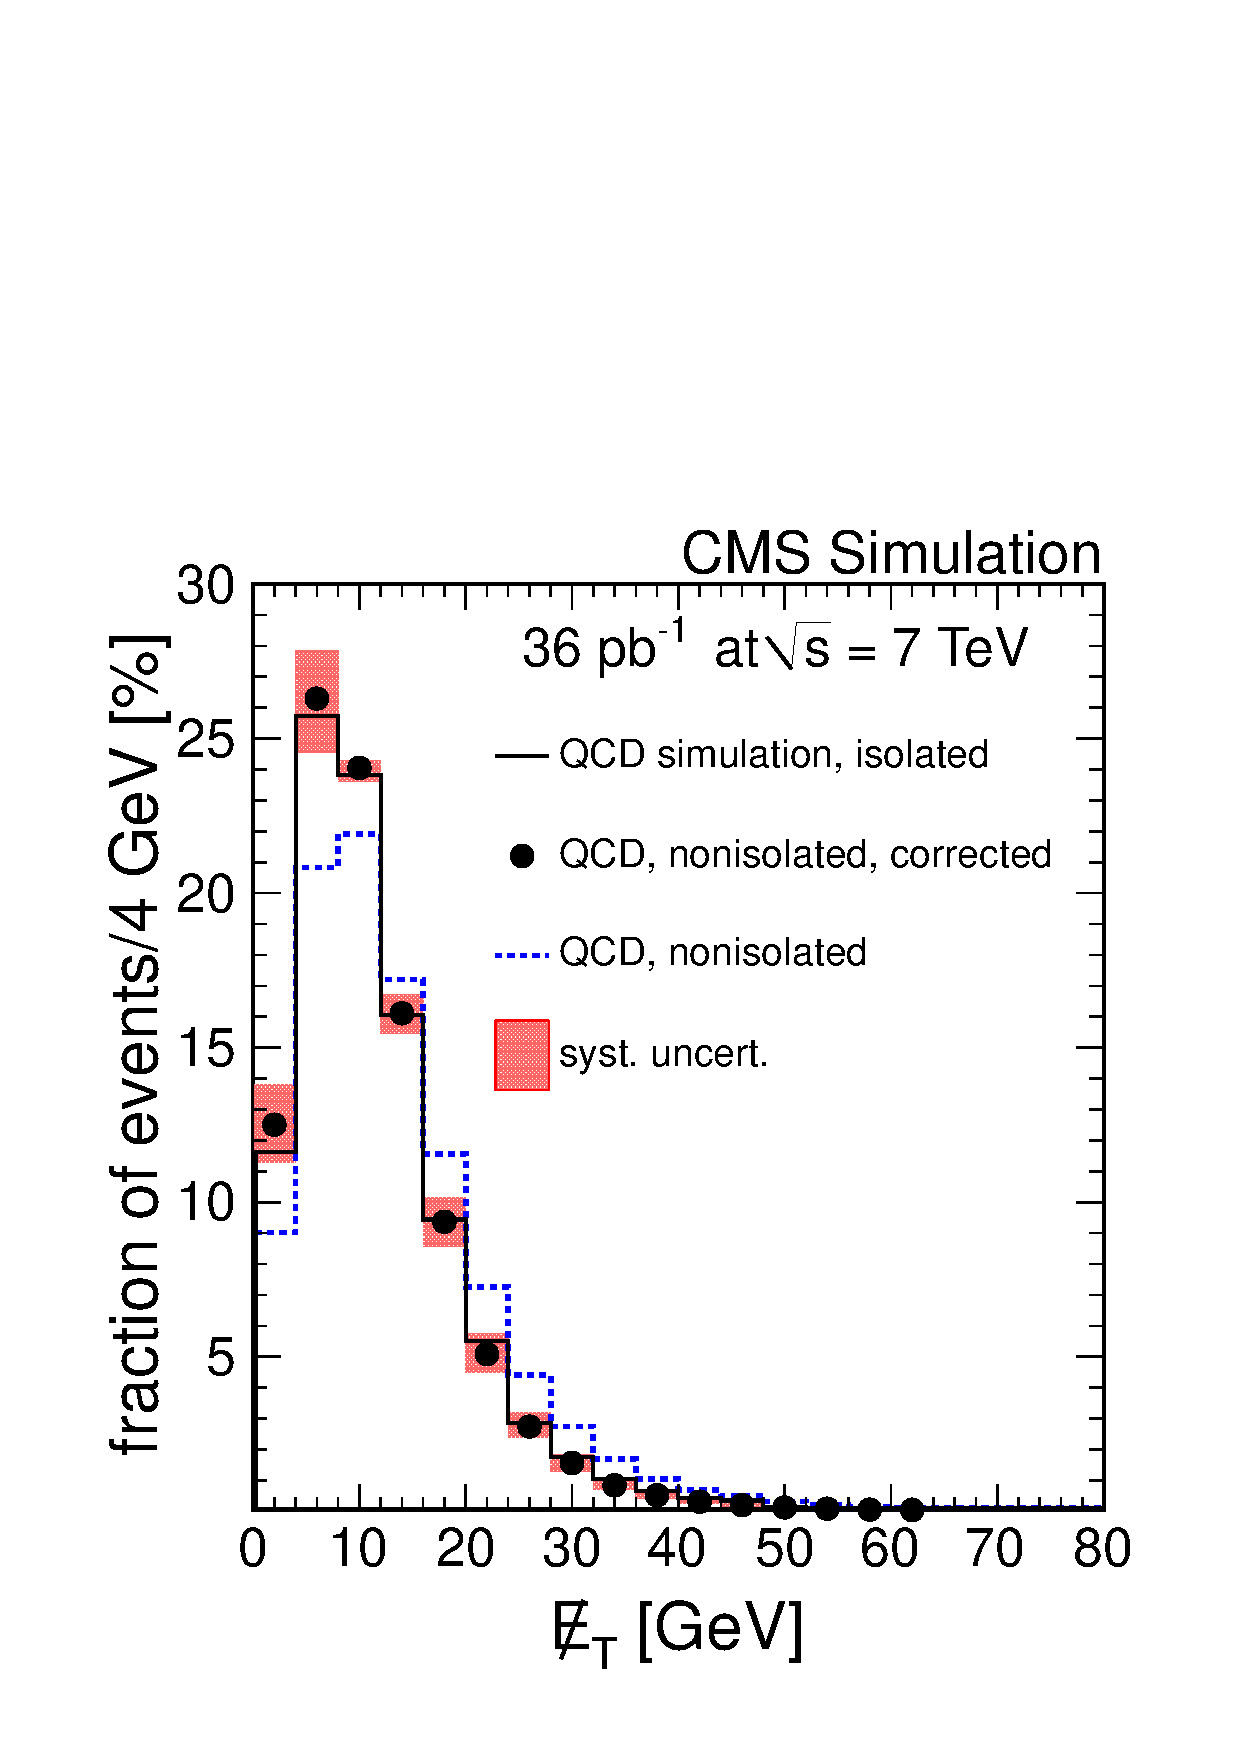
\includegraphics[width=7.5cm]{figs/qcd_template_MC.pdf}
    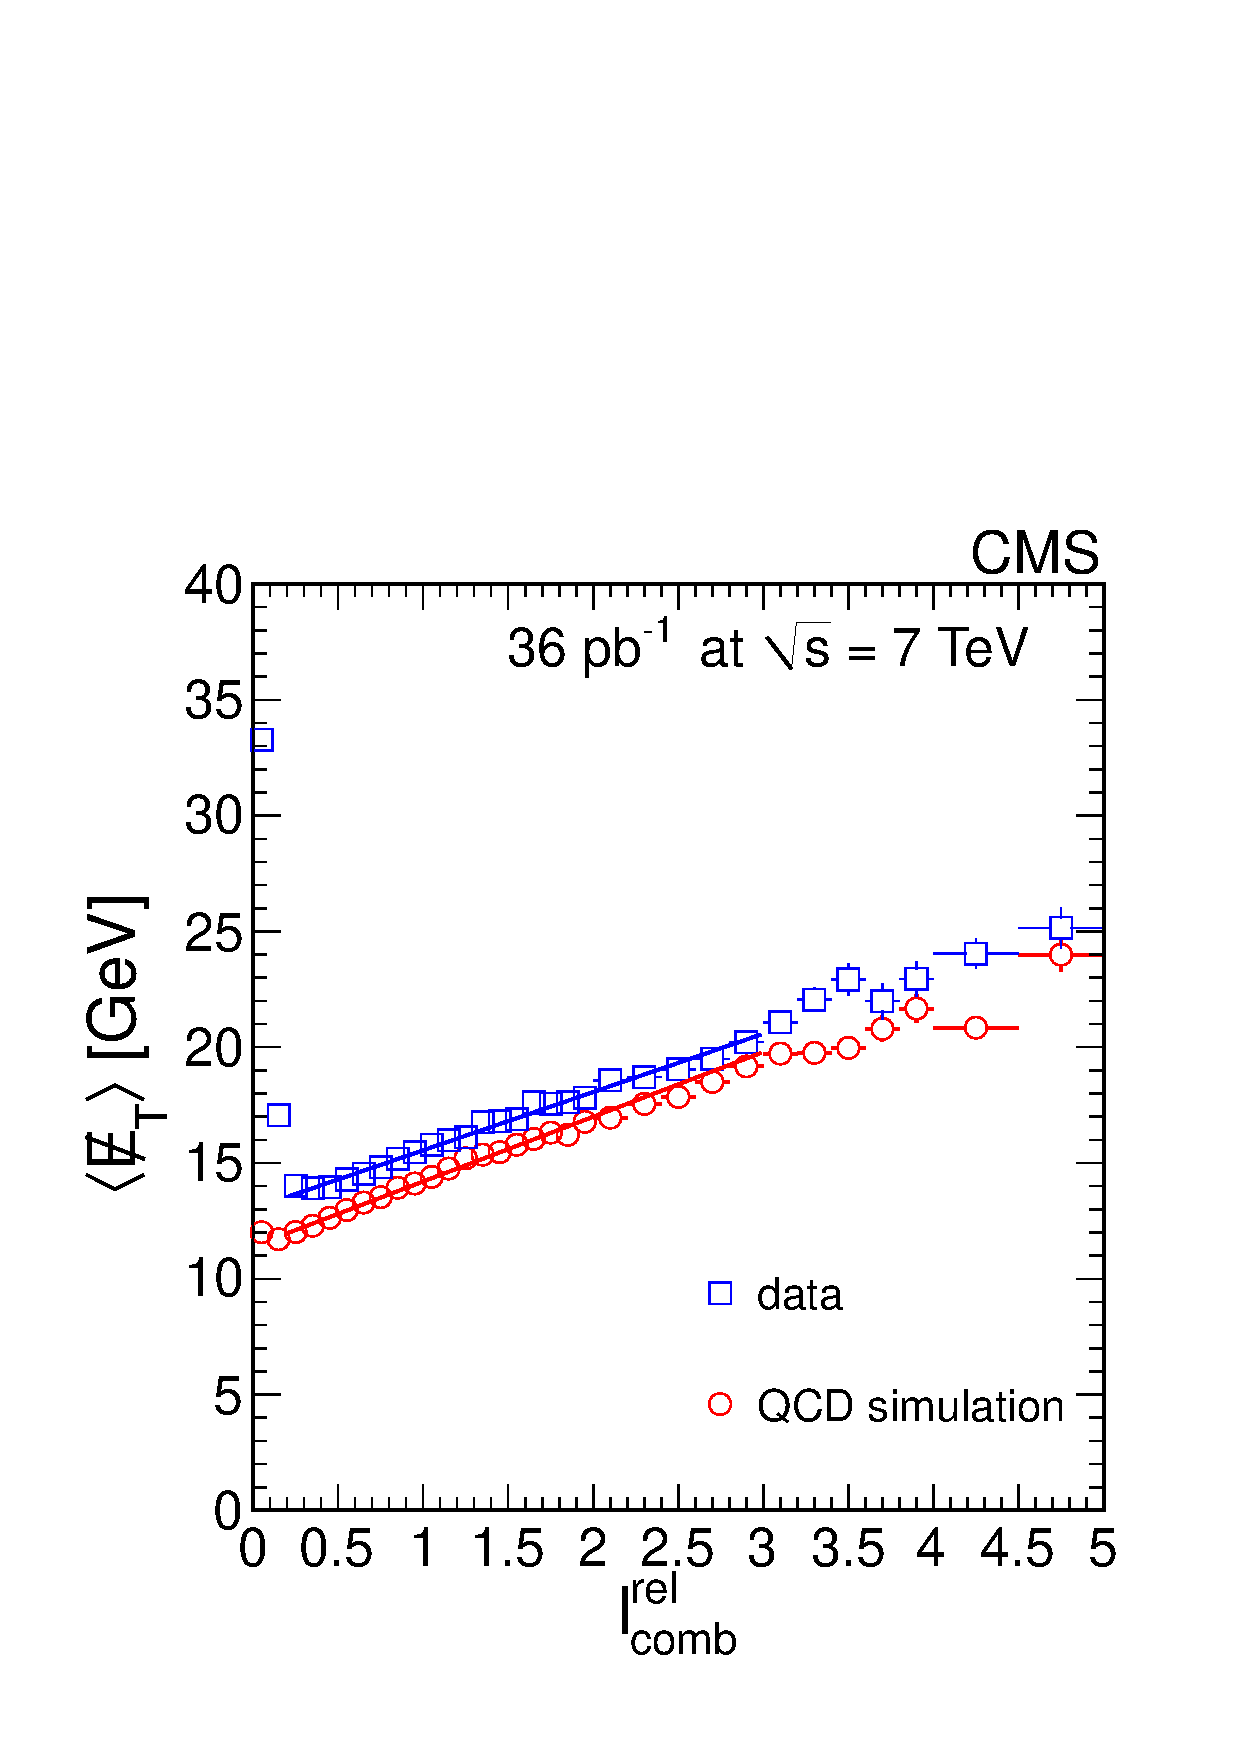
\includegraphics[width=7.5cm]{figs/Wmn_METvsIso.pdf}
    \caption{Left: distribution of the corrected $\MET$ for selected events
with a non isolated muon (black points) superimposed
on the distribution of uncorrected $\MET$ for the same events (blue, dashed line) and
$\MET$ for events with an isolated muon (black, solid histogram). All distributions are from simulated QCD events.
The shaded area represents the systematic uncertainty due to corrections
with factors $\alpha \pm \Delta \alpha$, for $\Delta \alpha = 0.08$.
Right: distribution of the average $\MET$ versus $\IRelComb$
for simulated QCD events (red circles) and
for data (blue squares).
The high values of $\MET$ in the first two bins in $\IRelComb$
are due to the presence of the W signal events. The superimposed lines are linear fits
in the range $[0.2, 3.0]$ of $\IRelComb$.
    \label{figure:Wmunu_QCD}}
}
\end{figure}
\begin{figure}[htbp]
{\centering
    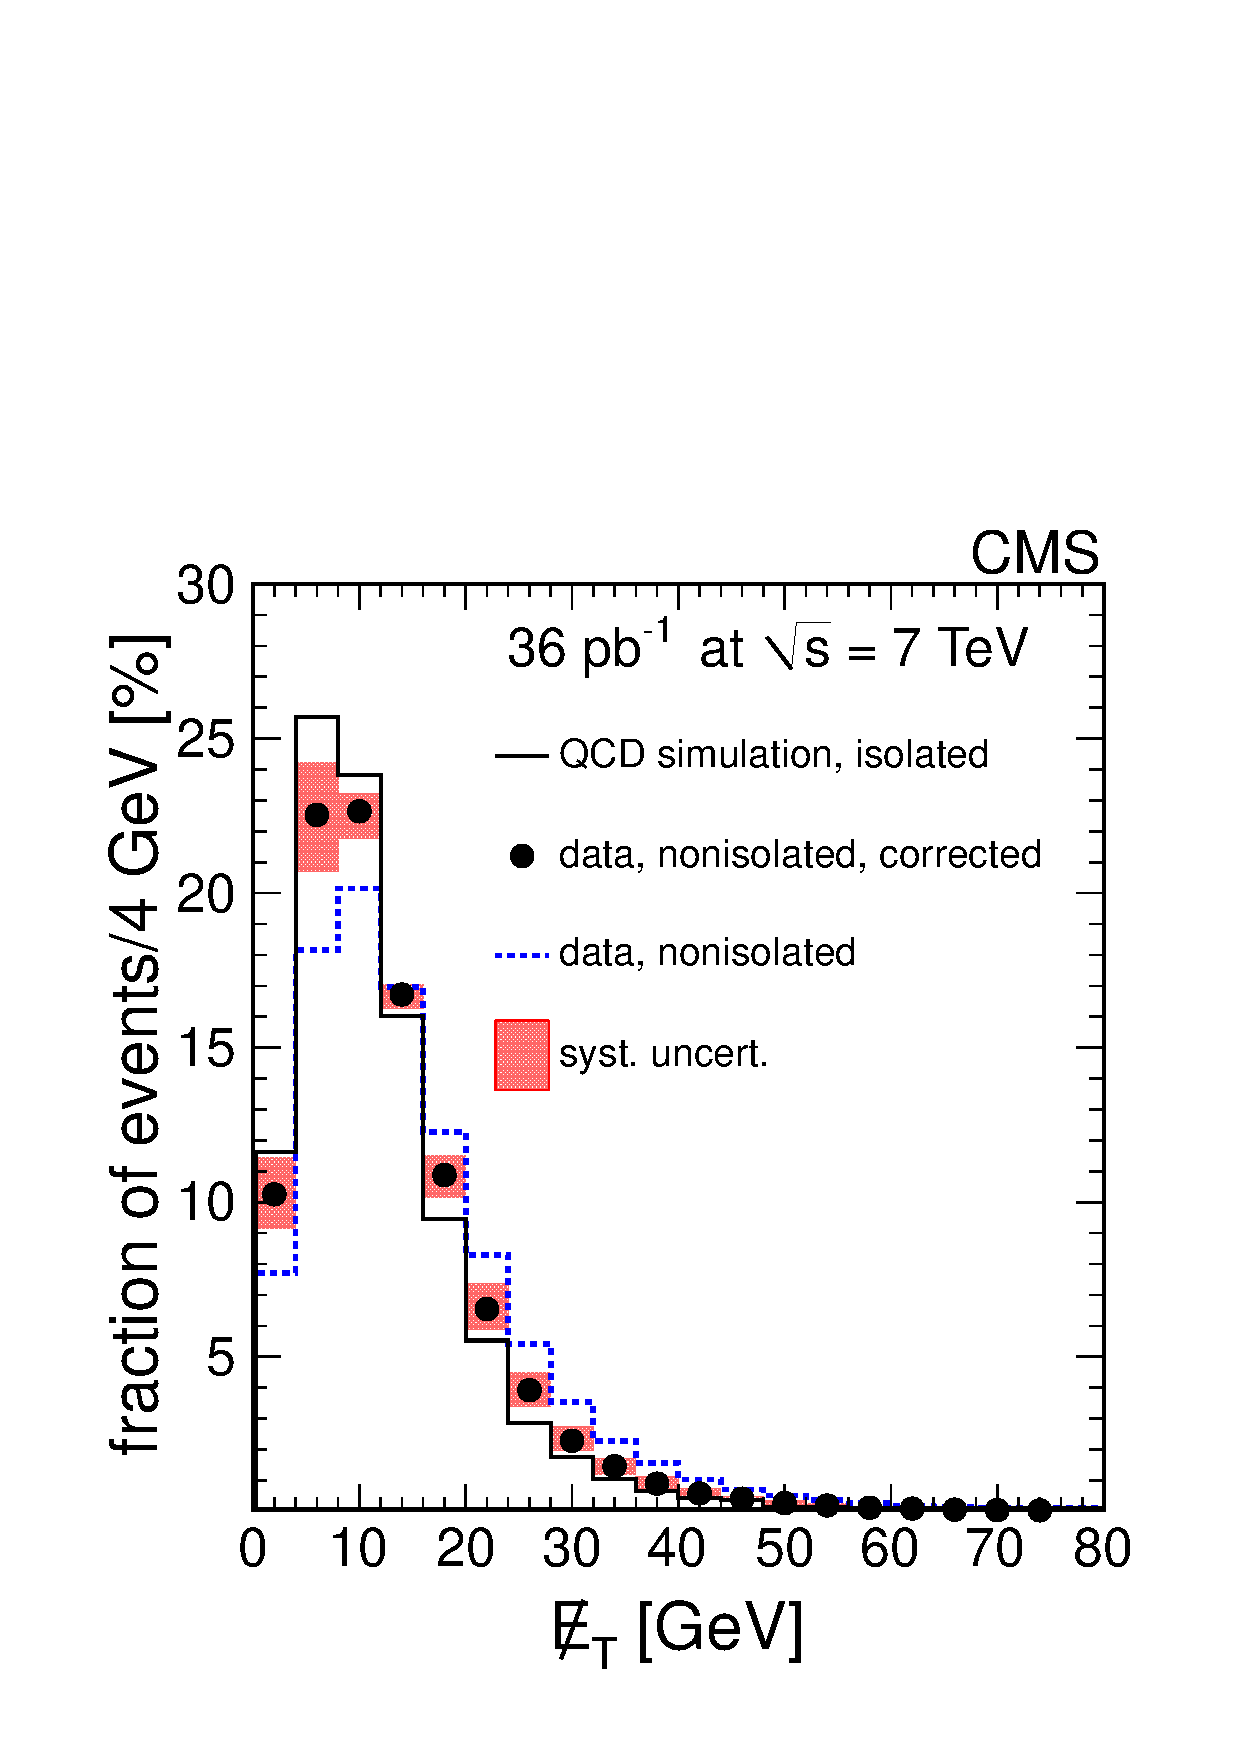
\includegraphics[width=7.5cm]{figs/qcd_template.pdf}
    \caption{
Distribution of the corrected $\MET$ for selected events
with a nonisolated muon in data (black points) superimposed
on the uncorrected $\MET$ distributions for data (blue dashed line) and
simulated QCD events (black, solid histogram, same as
the black, solid histogram in Fig.~\ref{figure:Wmunu_QCD}).
The shaded area represents the systematic uncertainty due to corrections with factors
$\alpha \pm \Delta \alpha$ for $\Delta \alpha = 0.08$.
    \label{figure:Wmunu_QCD_data}}
}
\end{figure}

The same positive correlation between $\MET$ and $\IRelComb$ is observed in the data
(blue squares in Fig.~\ref{figure:Wmunu_QCD}, right).
A correction $\MET^\prime = \MET/(1+\alpha\,\IRelComb)$, with $\alpha \approx 0.2$,
was applied.
The shapes obtained in data are shown in Fig.~\ref{figure:Wmunu_QCD_data} where
the uncorrected and corrected data shapes from events selected by inverting the isolation requirement, together with the
simulation expectation for events with an isolated muon, are shown.
The shaded area in Fig.~\ref{figure:Wmunu_QCD_data} is bounded by the two distributions, obtained using two extreme correction
parameters $\alpha \pm \Delta \alpha$, with $\Delta \alpha = 0.08$, as evaluated in simulations.
This area is taken as a systematic uncertainty on the QCD background shape.

Several parameterizations for the correction are considered,
but the impact on the corrected distribution and therefore on the final result is small.
Associated uncertainties on the cross section and ratios are evaluated as the differences between
the fit results obtained with the optimal $\alpha$ value and
two extreme cases, $\alpha \pm \Delta \alpha$.


The following signal yields are obtained: $140\,757 \pm 383$ for the inclusive sample,
$56\,666\pm240$ for the $\Wmmn$ sample, and $84\,091\pm291$ for the $\Wpmn$ sample.

The $\MET$ distributions are presented in
Fig.~\ref{figure:Wmunu_exp_fit} (full sample) and Fig.~\ref{figure:Wmn_PlusMinus}
 (samples selected by the muon charge) superimposed on the individual fitted
contributions of the W signal and the EWK and QCD backgrounds.
Figures~\ref{figure:Wmunu_exp_fit} and~\ref{figure:Wmn_PlusMinus}
show the $\MET$ distributions for data and fitted signal, plus background components.
 Figure~\ref{figure:Wmunu_exp_fit_mt}
% and~\ref{figure:Wmn_PlusMinus_mt}
shows the $\MT$ distributions for data and signal, plus background components, fitted
from the $\MET$ spectra.

% The fitted W parameters are summarized in Tables~\ref{table:Wmunu_tot_xs}
% for the two choices of fit parameters. The error shown is only statistical.
 \begin{figure}[!ht] {\centering
   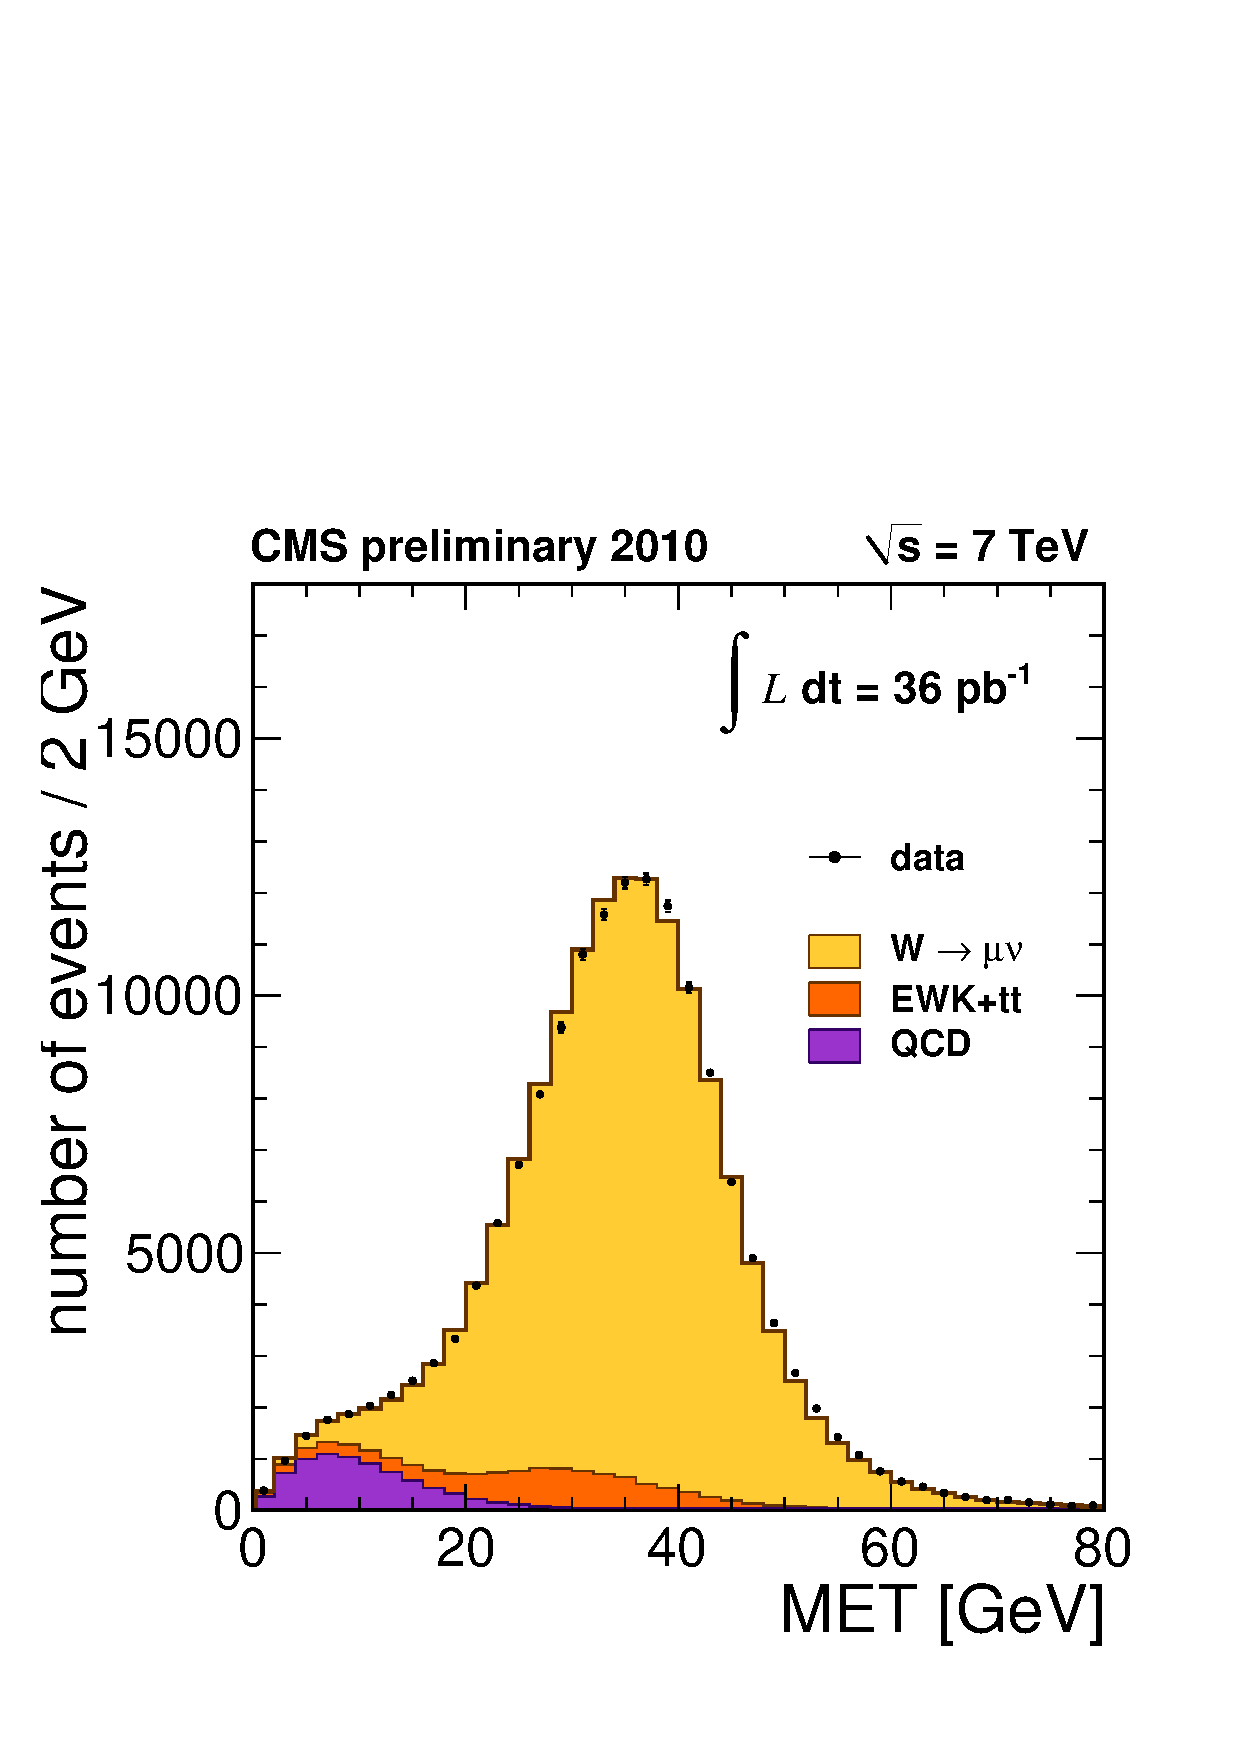
\includegraphics[width=7cm]{figs/Wmn_MET.pdf}
   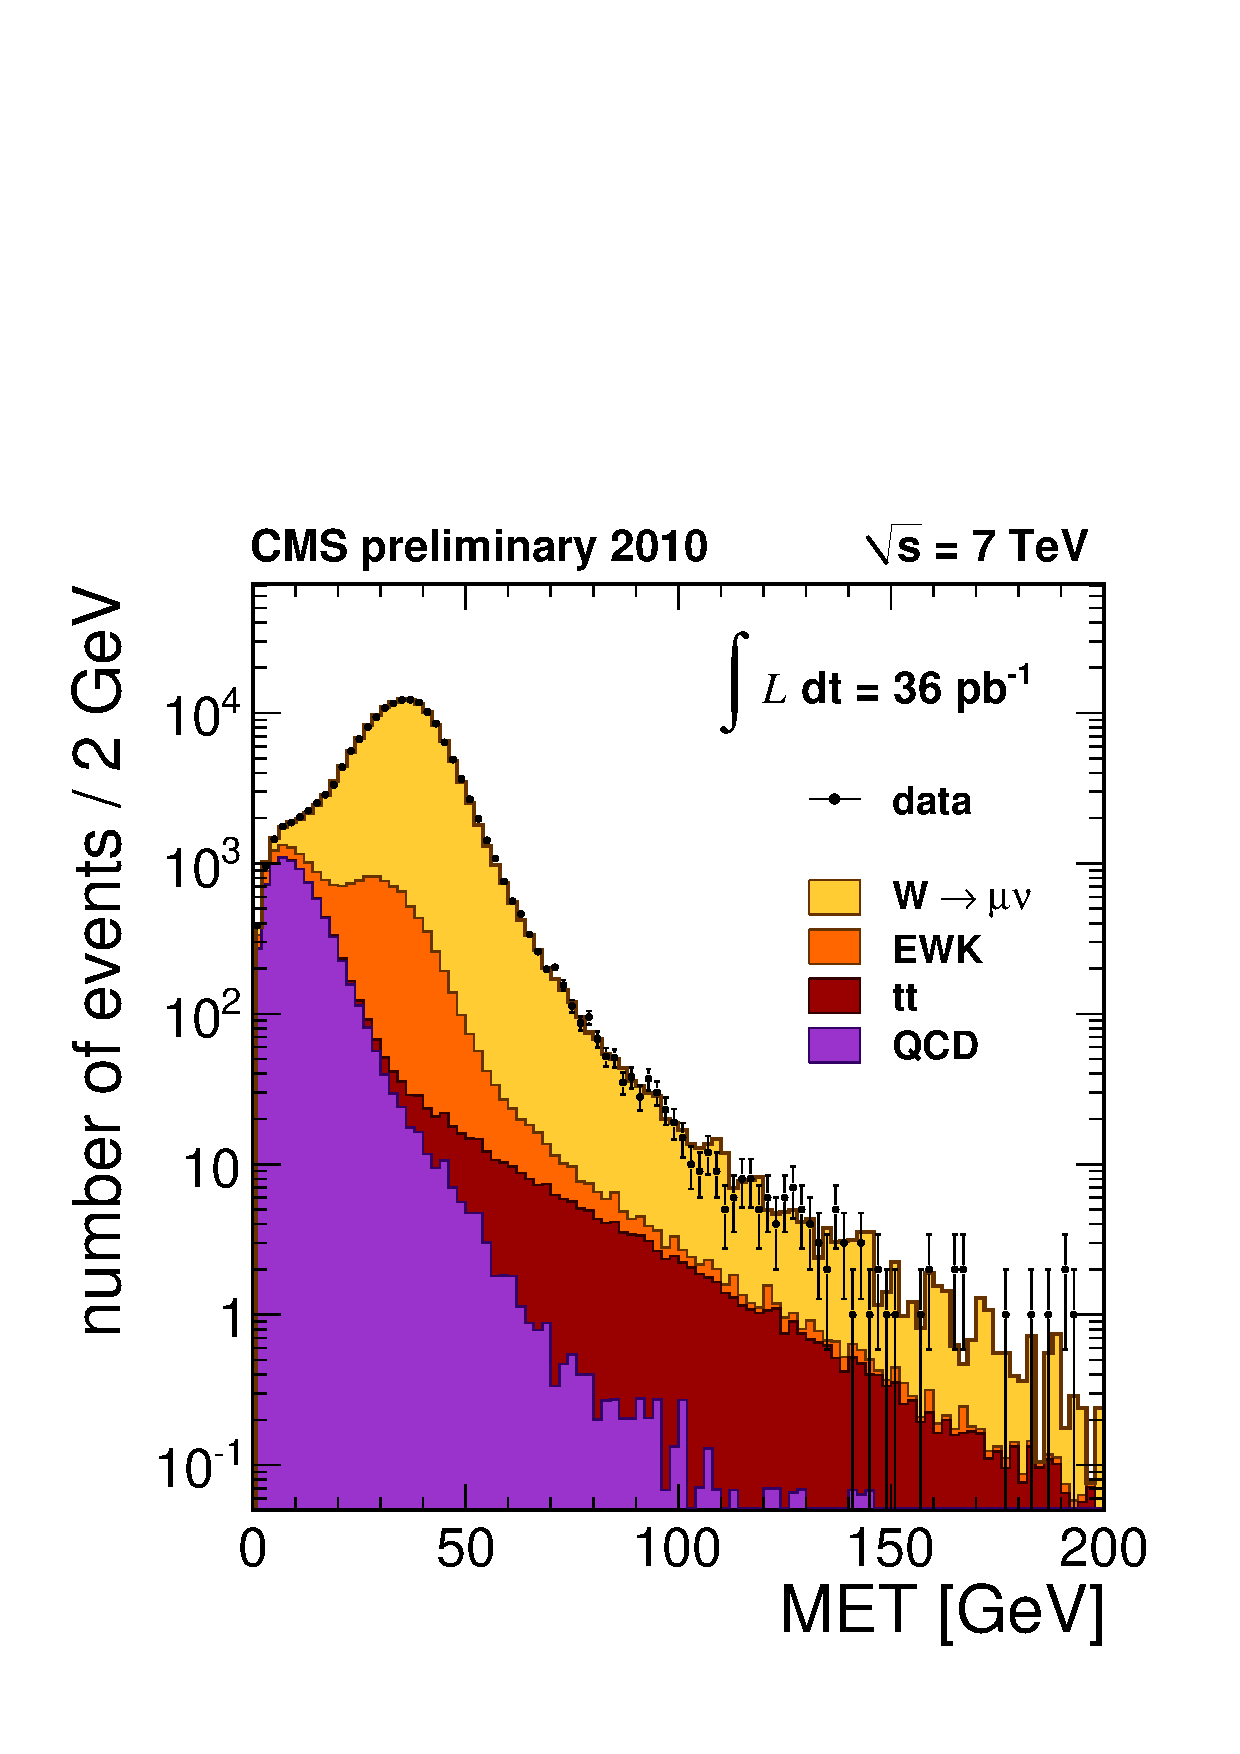
\includegraphics[width=7cm]{figs/Wmn_MET_log.pdf}
     \caption{
The $\MET$ distribution for the selected $\Wmn$ candidates on
a linear scale (left) and on a logarithmic scale (right).
The points with the error bars represent the data. Superimposed are the
contributions obtained with the fit
for QCD background (violet, dark histogram), all other backgrounds
(orange, medium histogram), and signal plus  background (yellow, light histogram).
The black dashed line is the fitted signal contribution.
     \label{figure:Wmunu_exp_fit}}
}
 \end{figure}

\begin{figure}[!ht] {\centering
   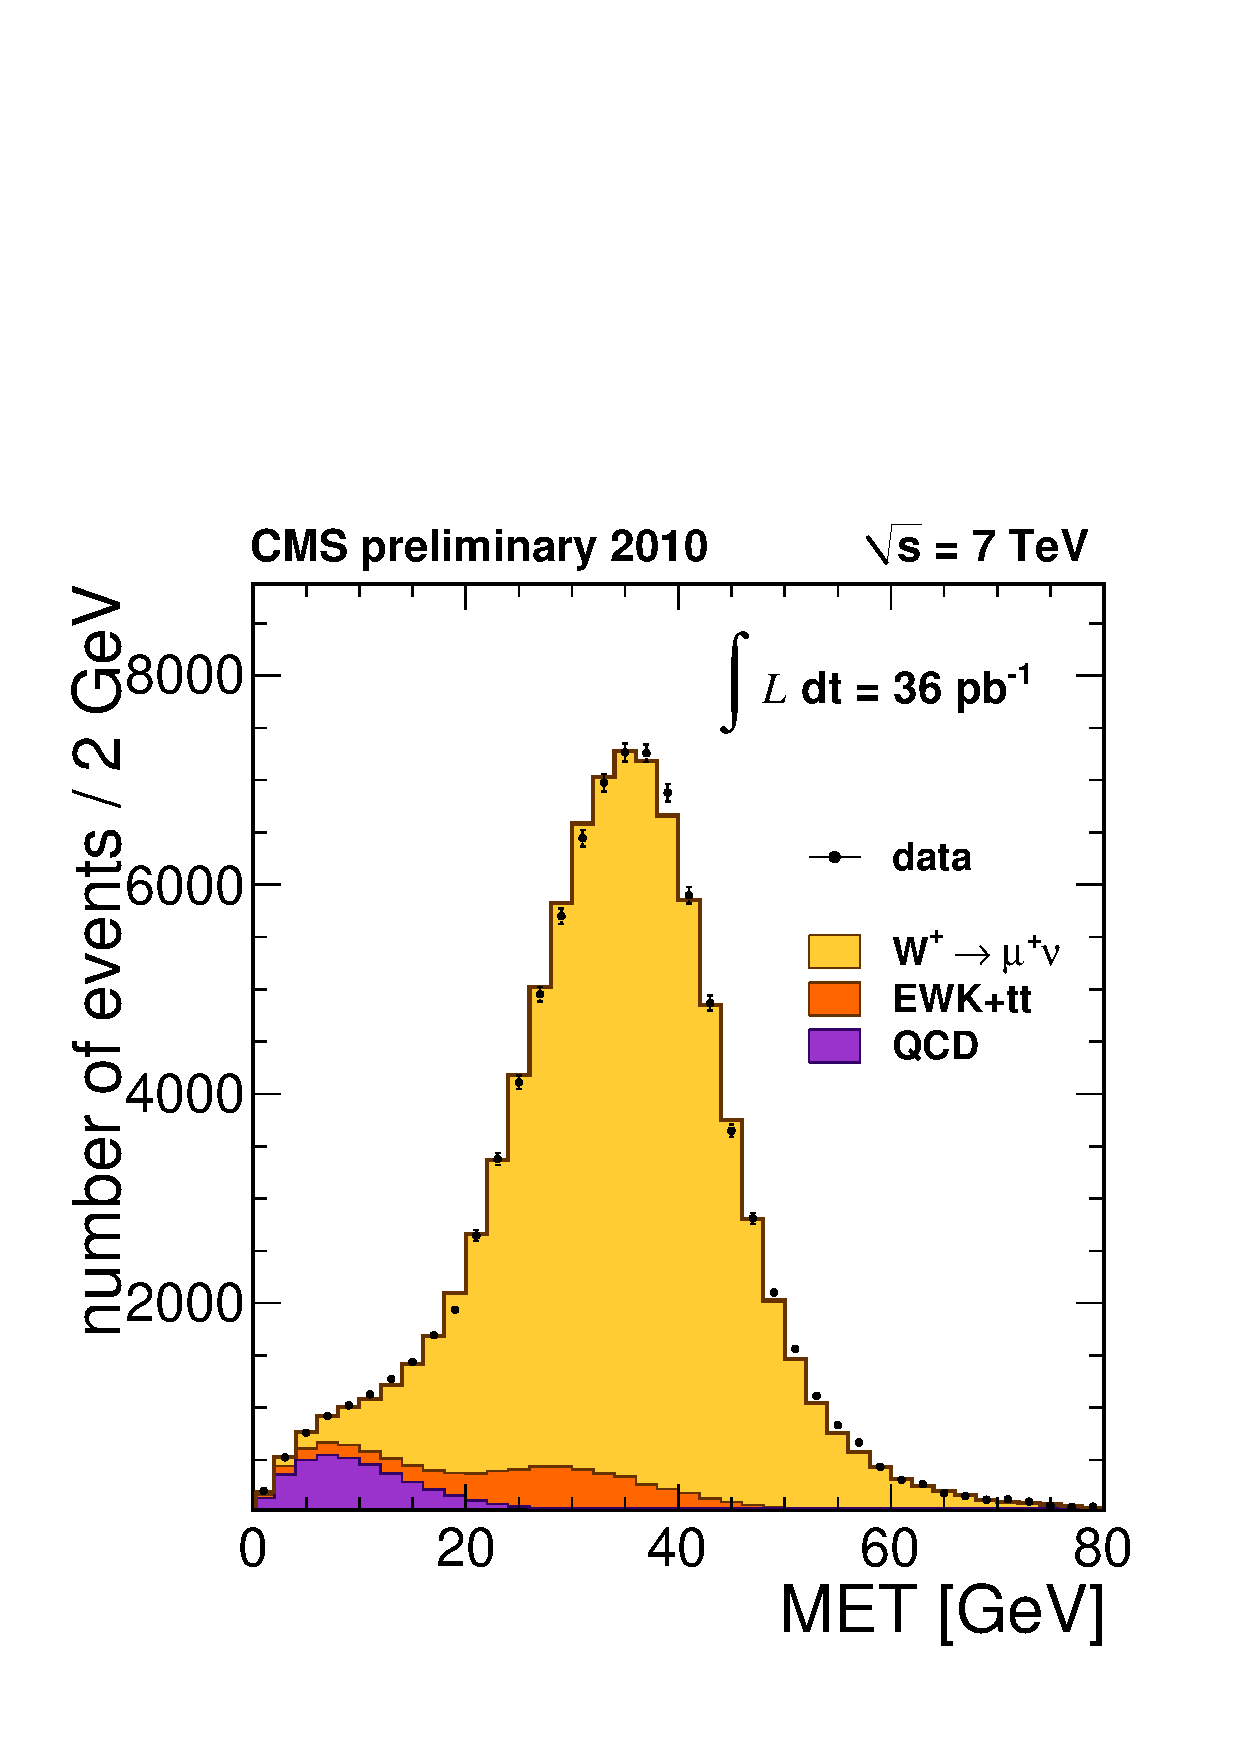
\includegraphics[width=7cm]{figs/Wmn_MET_plus.pdf}
   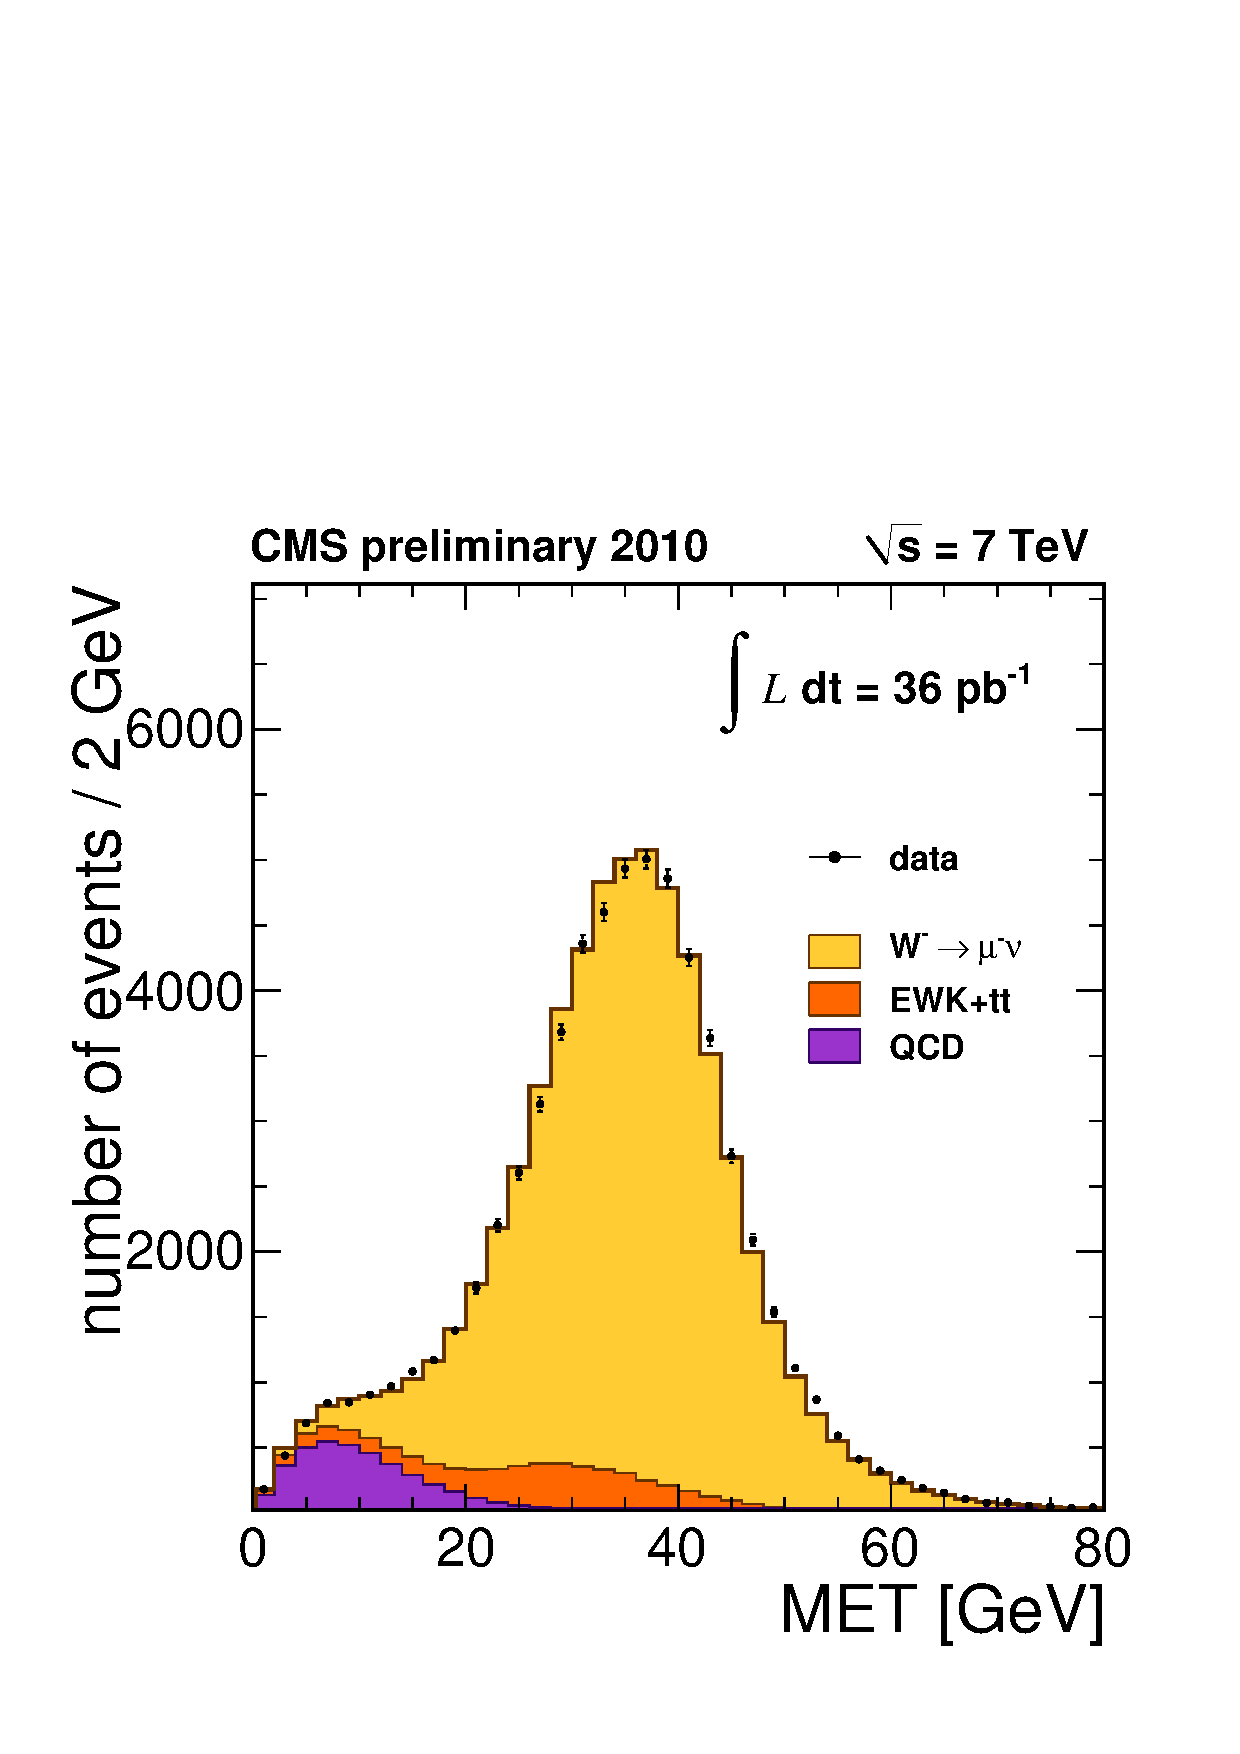
\includegraphics[width=7cm]{figs/Wmn_MET_minus.pdf}
    \caption{
The $\MET$ distributions for the selected W$^+$ (left) and W$^-$ (right) candidates.
The points with the error bars represent the data. Superimposed are the contributions
obtained with the fit for QCD background (violet, dark histogram), all other backgrounds
(orange, medium histogram), and signal plus background (yellow, light histogram).
The black dashed line is the fitted signal contribution.
    \label{figure:Wmn_PlusMinus}}
}
\end{figure}

 \begin{figure}[!ht] {\centering
   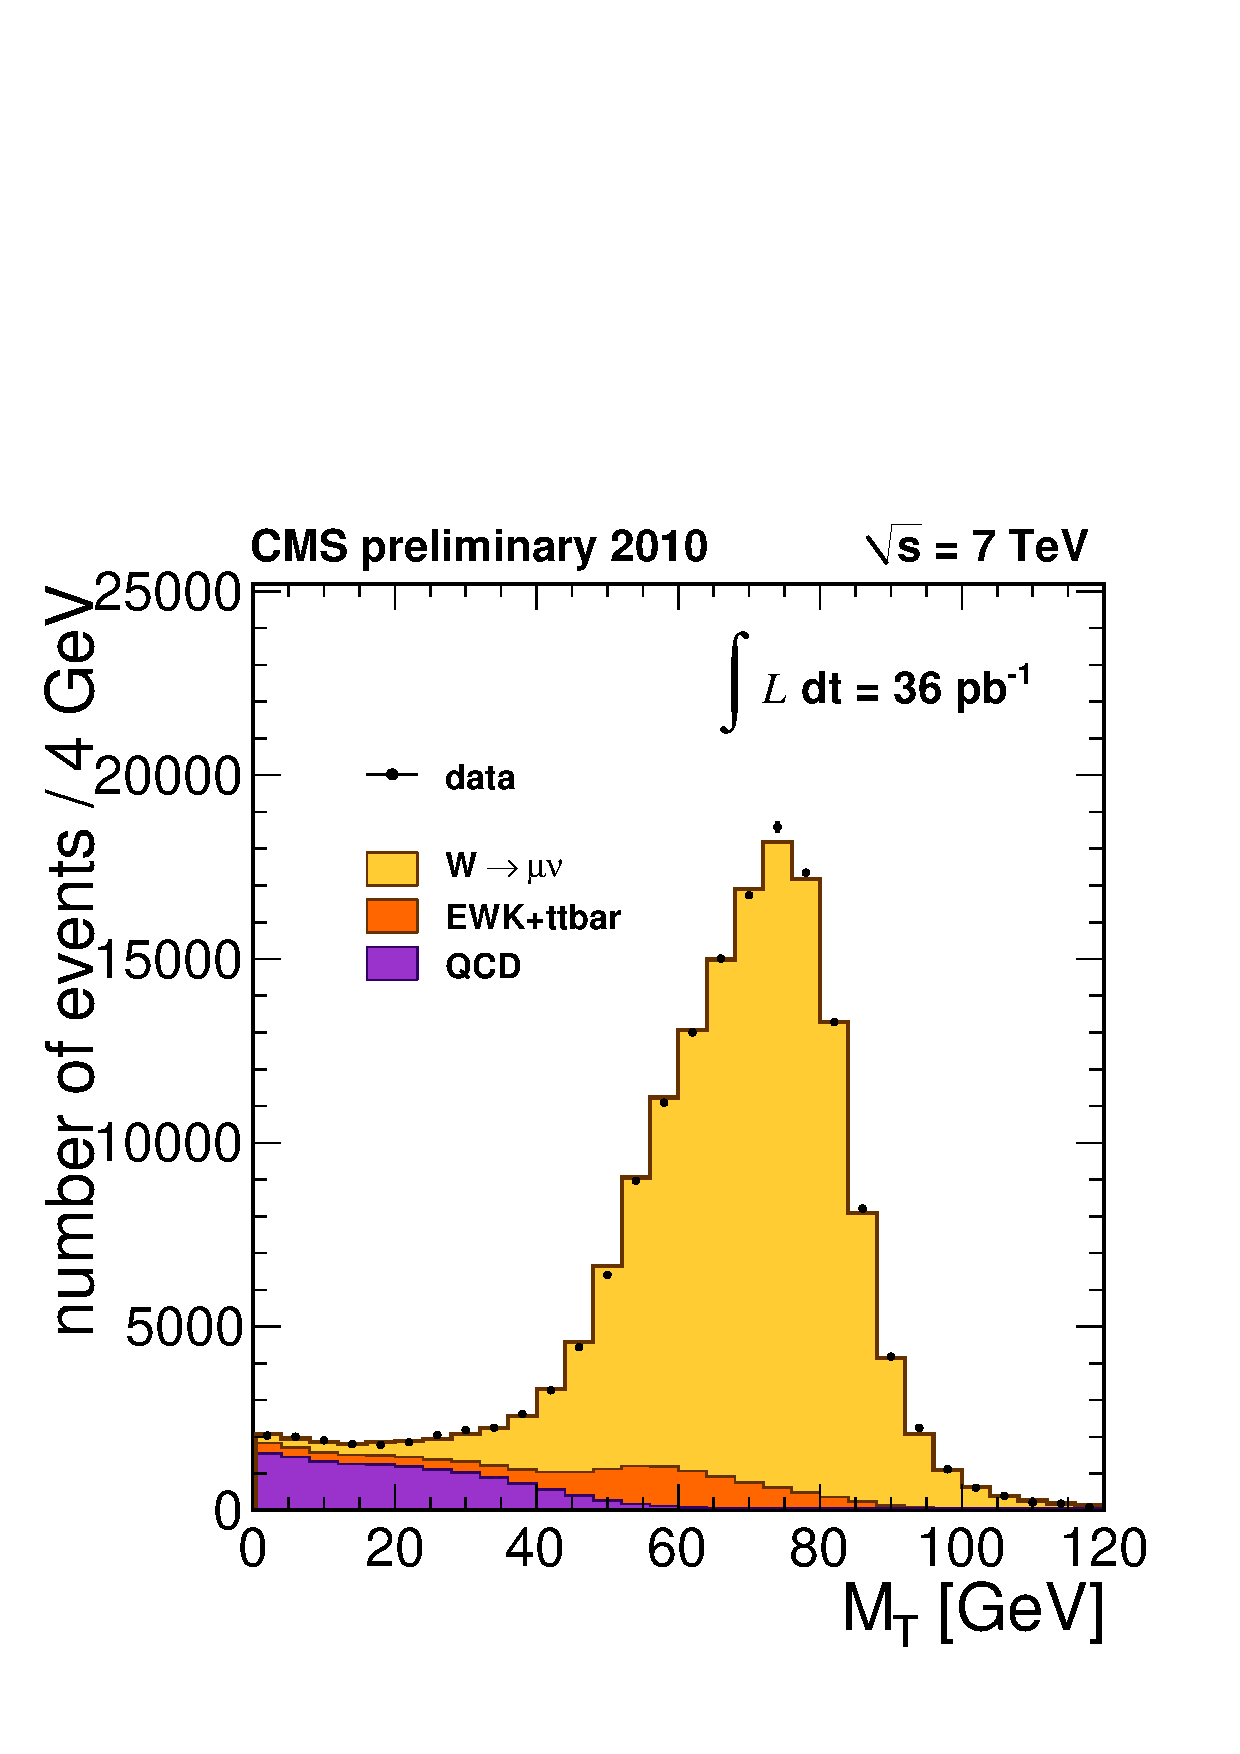
\includegraphics[width=7cm]{figs/Wmn_MT.pdf}
   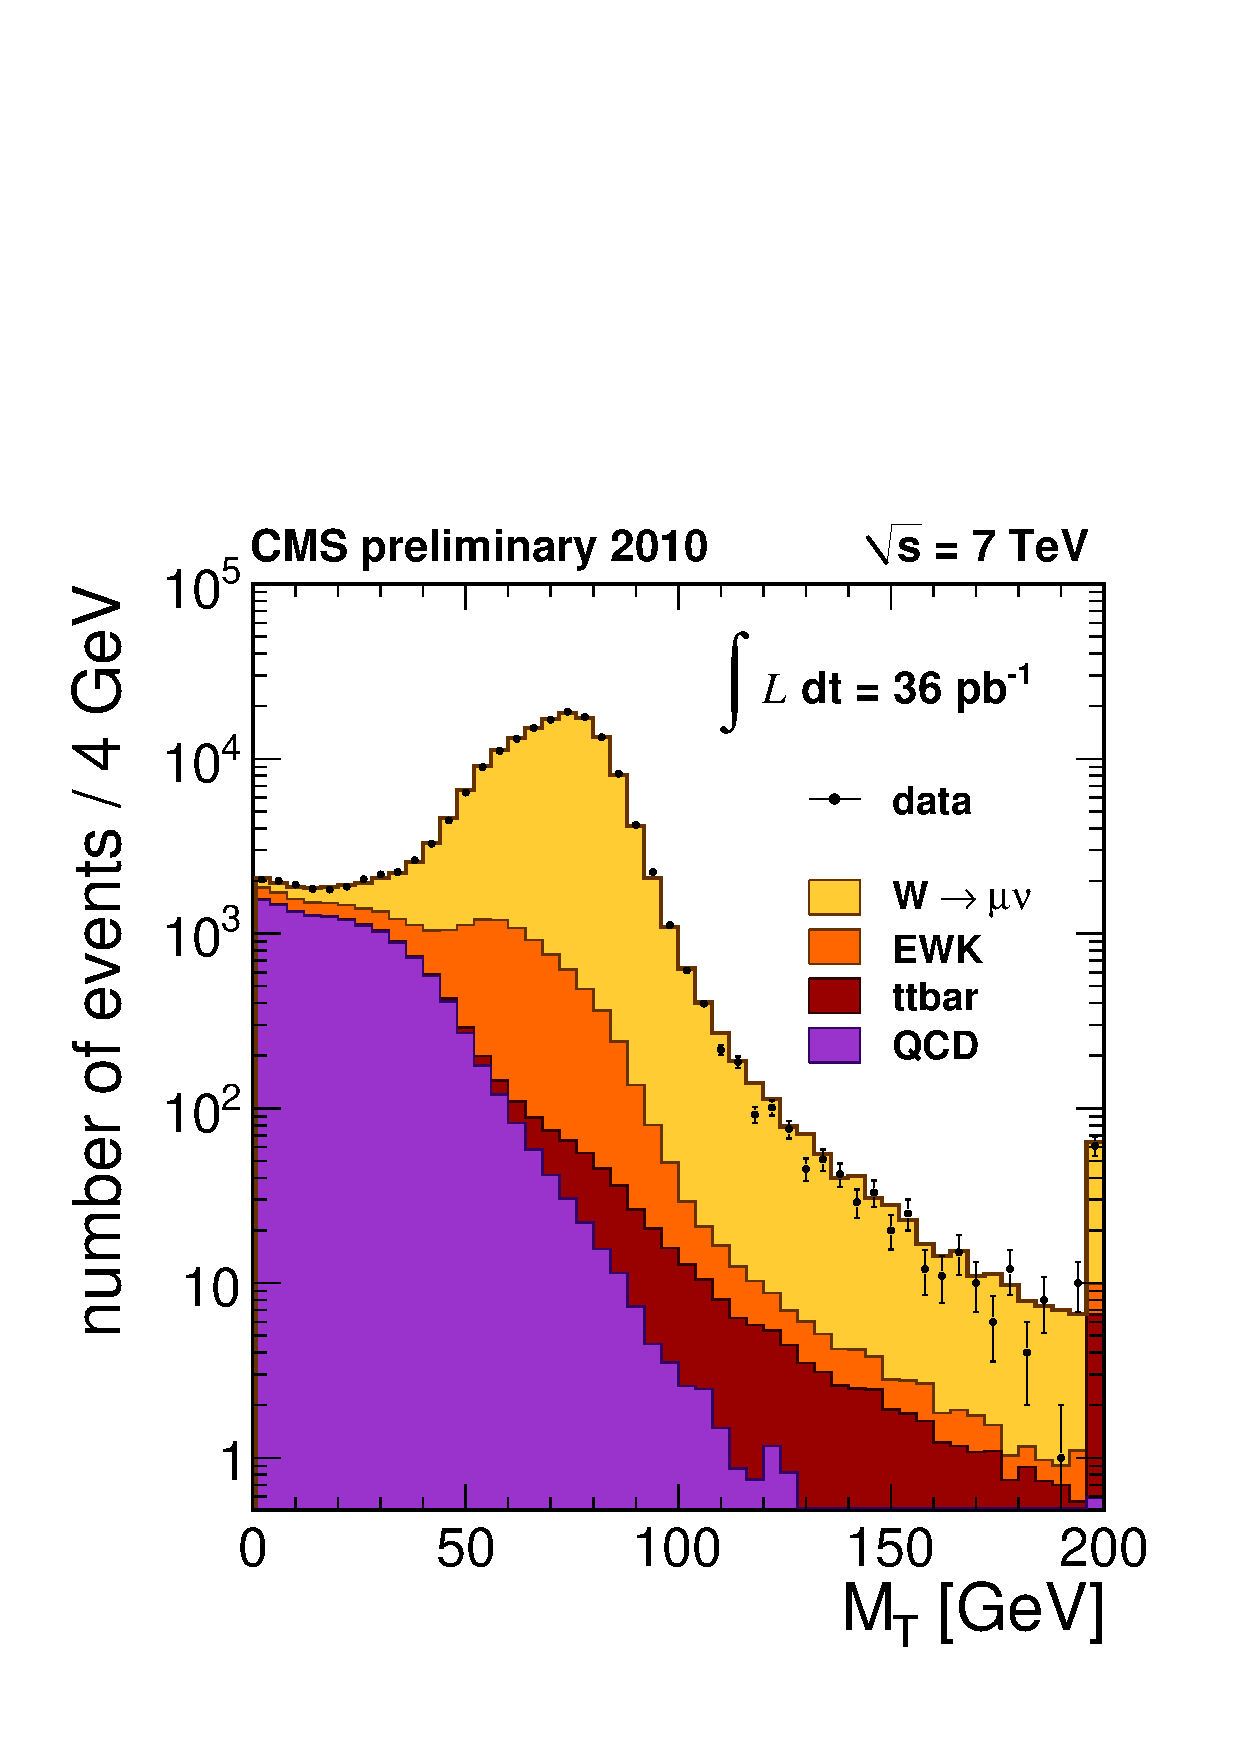
\includegraphics[width=7cm]{figs/Wmn_MT_log.pdf}
     \caption{
The $\MT$ distribution for the selected $\Wmn$ candidates on
a linear scale (left) and on a logarithmic scale (right).
The points with the error bars represent the data. Superimposed are the
contributions obtained with the fit
for QCD background (violet, dark histogram), all other backgrounds
(orange, medium histogram), and signal plus background (yellow, light histogram).
The black dashed line is the fitted signal contribution.
     \label{figure:Wmunu_exp_fit_mt}}
}
 \end{figure}

\subsection{\texorpdfstring{The $\Zee$ Signal Extraction}{The Z->ee Signal Extraction}}

In the following sections the use of a pure $\Zee$ sample
for the determination of the residual energy-scale and resolution corrections is first discussed.
Then the signal extraction with the counting analysis and the
simultaneous fit methods are presented.

\subsubsection{Electron Energy Scale}
\label{sec:e-escale}

The lead tungstate crystals of the ECAL are subject to transparency loss
during irradiation, followed by recovery in periods with no
irradiation. The magnitude of the changes to the energy response is
dependent on instantaneous luminosity and was, at the end of the 2010
data taking period, up to 1$\%$ in the barrel region, and 4$\%$ or more in
parts of the endcap. The changes are monitored continuously by injecting
laser light and recording the response. The corrections derived from
this monitoring are validated by studying the variation of the $\pi^0$ mass
peak as a function of time for different regions of the ECAL (using $\pi^0$ data
collected in a special calibration stream), and by studying the overall $\Zee$ mass peak and width.
%The correction
%calculations are still being developed and commissioned, and the
%corrections provided for the current reconstruction do not yet achieve
%the target precision. However, the validation and testing show that the
%residual variation of the energy scale with time, using these
%corrections, is less than 0.3$\%$ in the barrel and less than 1$\%$ in the
%endcap.
%
% from Isabel
%
With the current corrections, residual variations of the energy scale with time are
at the level of 0.3\% in the barrel and less than 1\% in the endcaps.


\par
%
% Isabel suggests to rewrite this section
%
%
The remaining mean scale correction factors to be applied to the data and the
resolution corrections (smearing) to be applied to the simulated sample
are estimated from $\Zee$ events. Invariant mass distributions for electrons
in several $\eta$ bins in the EB and EE are derived
from simulations and compared to data. A simultaneous fit of a Breit--Wigner convolved with a
Crystal-Ball function to each $\Zee$ mass distribution is performed  in order
to determine the energy scale correction factors for the data and the resolution
smearing corrections for the simulated samples. The energy scale correction
factors are below 1$\%$ while the resolution smearing corrections are below 1$\%$
everywhere, with the exception of the transition region between the EB and the EE,
where they reach 2$\%$.
Those corrections are propagated in the analysis and proper systematic uncertainties
for the cross section measurements are estimated as discussed in Section~\ref{subsec:ELEsystematics}.
%
%
% The remaining mean scale correction factors to be applied to the data and the
% resolution correction (smearing) to be applied to the simulated sample
% are estimated as follows.
% The $\Zee$ events are divided into categories that correspond to all possible
% combinations of four $\eta$ bins in the EB and two $\eta$ bins in the EE.
% An invariant mass distribution is derived from simulations in each category.
% A simultaneous fit of a Breit-Wigner convolved with a Crystal-Ball function
% to the $\Zee$ mass distribution is performed in each of the $\eta$ bins, in order
% to determine the energy scale correction factors for the data and the resolution
% smearing correction factors for the simulated samples.
% The energy scale correction factors for the data and the resolution smearing correction
% factors for the simulated samples for the tight selection are reported
% in Table~\ref{tab:EnergyScaleResolution}.
%
% \begin{table}[ht] %
%   \begin{center}
%   \caption{ Energy scale correction factors for the data and
% resolution smearing correction factors for the simulated samples
% to be applied per electron for various $\eta$ bins.
%   \label{tab:EnergyScaleResolution}}
%   \begin{tabular}{|l|c|c|}
%     \hline
%     Region  & Energy scale & Resolution Correction (smearing) [GeV] \\
%     \hline\hline
% $0.0<|\eta|<0.4$ & $0.9940\pm0.0010$ & $0.29\pm0.20$ \\
% $0.4<|\eta|<0.8$ & $0.9958\pm0.0011$ & $0.30\pm0.23$ \\
% $0.8<|\eta|<1.2$ & $0.9992\pm0.0012$ & $0.37\pm0.22$ \\
% $1.2<|\eta|<1.5$ & $1.0079\pm0.0020$ & $1.07\pm0.19$ \\
% $1.5<|\eta|<2.0$ & $0.9955\pm0.0019$ & $1.04\pm0.22$ \\
% $2.0<|\eta|<2.5$ & $1.0003\pm0.0013$ & $0.18\pm0.15$ \\
%     \hline
%     \end{tabular}
%   \end{center}
% \end{table}

\par
%
% This probably deserves to be put in a separate section instead of "Electron energy Scale"
% (Luca)
%
\subsubsection{Counting Analysis}
After energy scale corrections, applied to electron ECAL clusters before
any threshold requirement, 10 fewer events ($-0.12\%$) were selected compared to the number of selected
events before the application of the energy scale corrections.
This brings the final $\Zee$ sample to $\ZEESAMPLEN$ and, after
background subtraction, the $\Zo$ yield is $\ZEEYIELD$ events.
This yield is used for the cross section estimation.
%
% If this is not the result of the fit but just the counting
%


\par
The dielectron invariant mass spectra for the selected sample
with the tight selection before and after the application of the corrections are
shown in Fig.~\ref{fig:Zee} along with the predicted distributions.
The data and simulation distributions are normalized to account for the difference in selection
efficiency.

%%%%%
\begin{figure}
  \begin{center}
   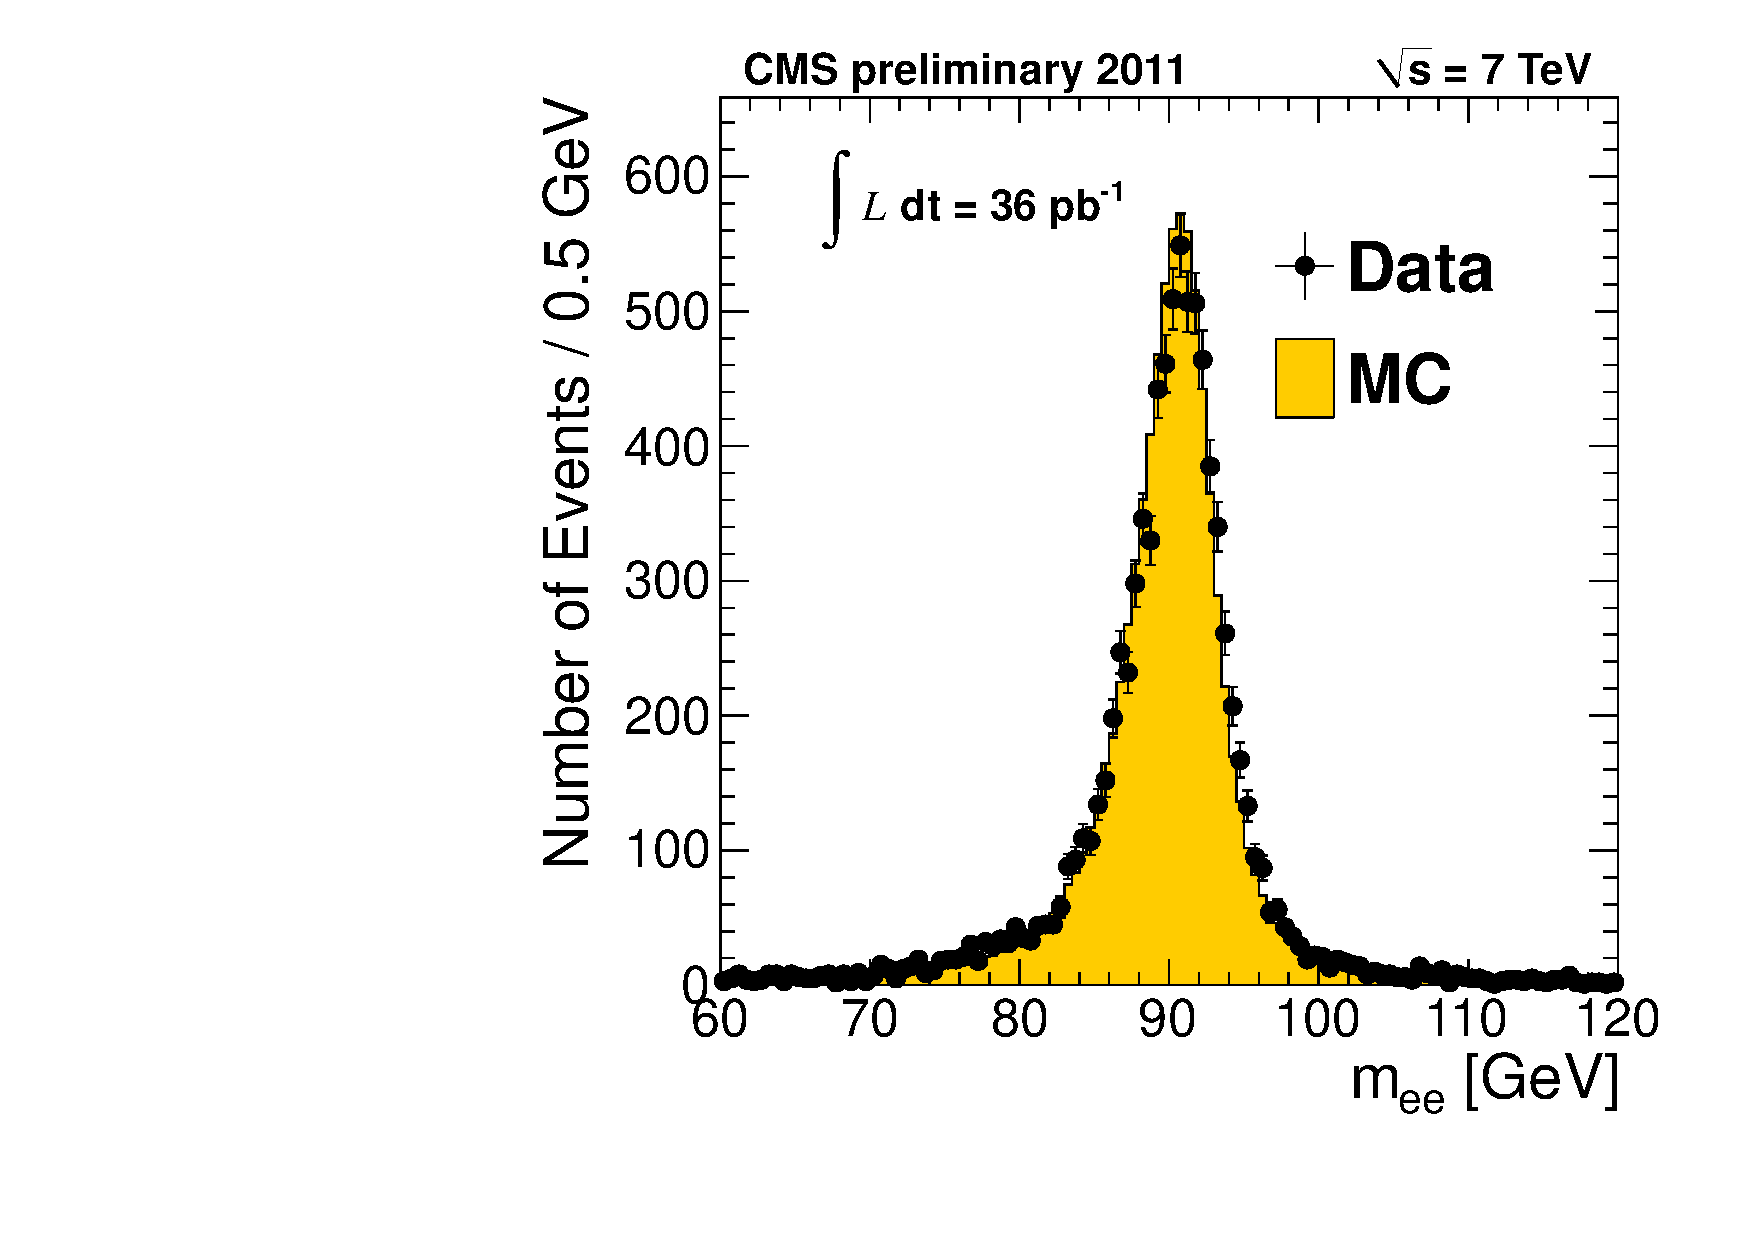
\includegraphics[width=0.48\textwidth]{figs/Zee_mass_Linear.pdf}
   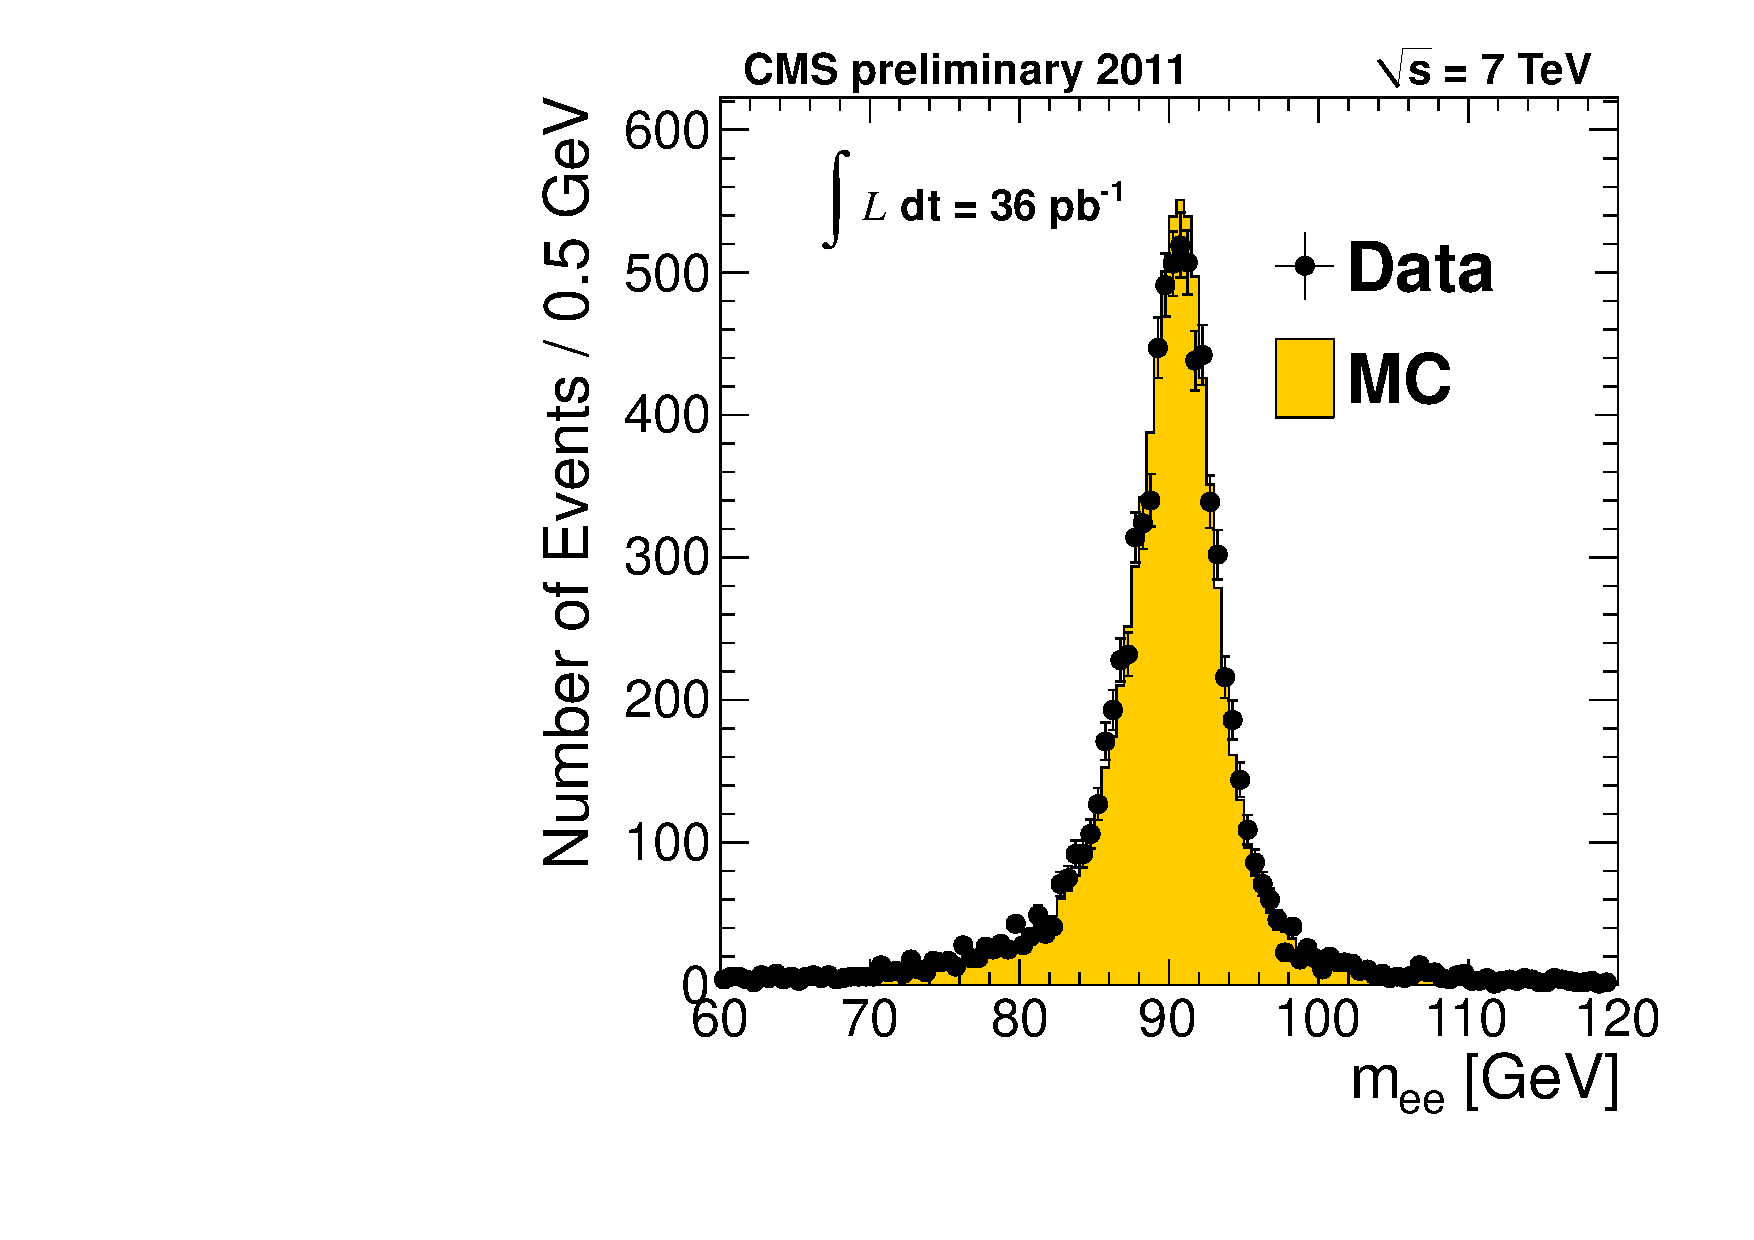
\includegraphics[width=0.48\textwidth]{figs/Zee_mass_Linear_corrected.pdf}
   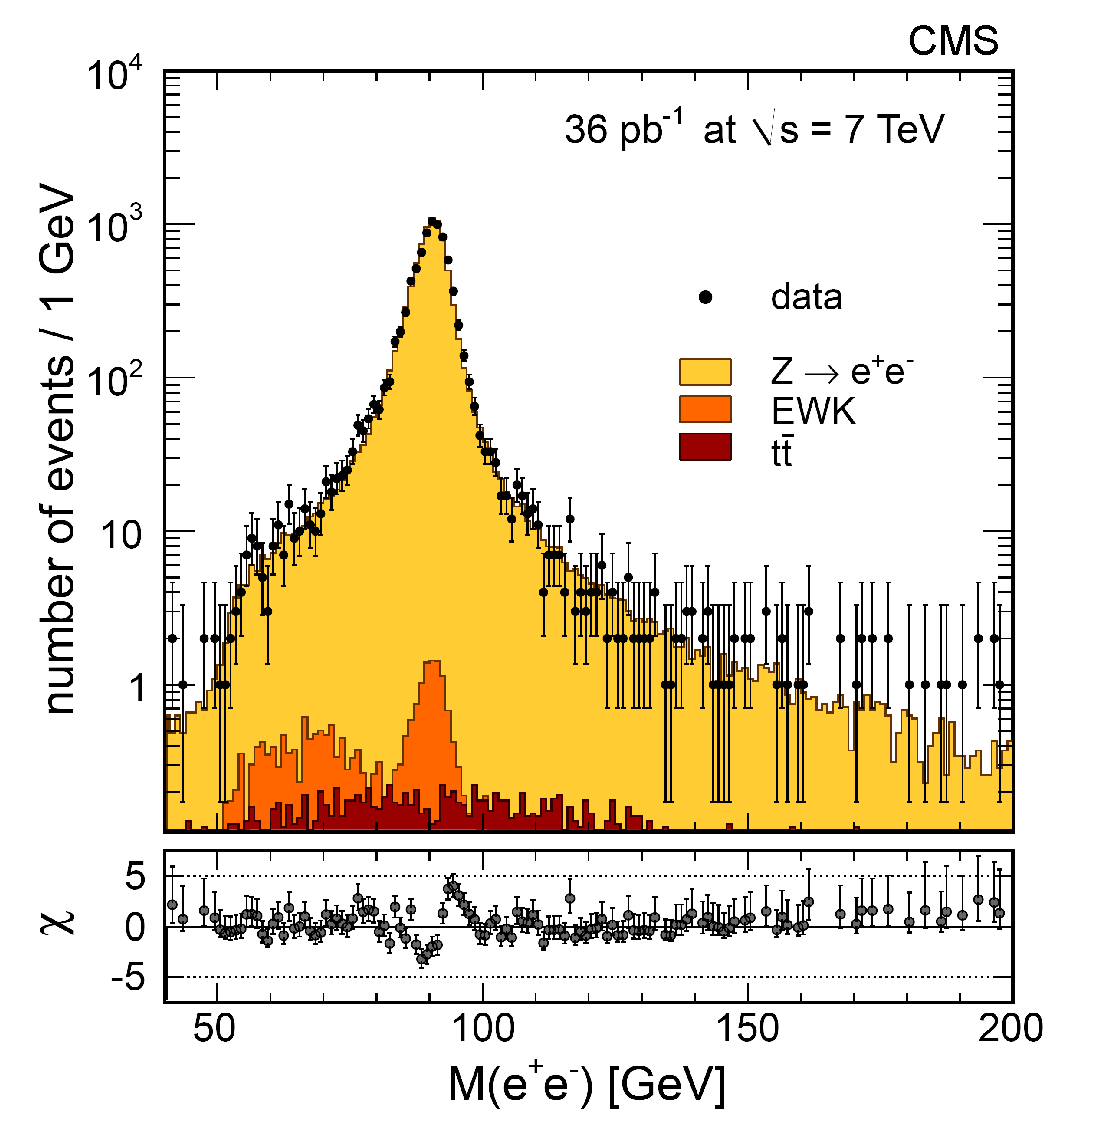
\includegraphics[width=0.48\textwidth]{figs/Zee_mass_Logarithmic.pdf}
   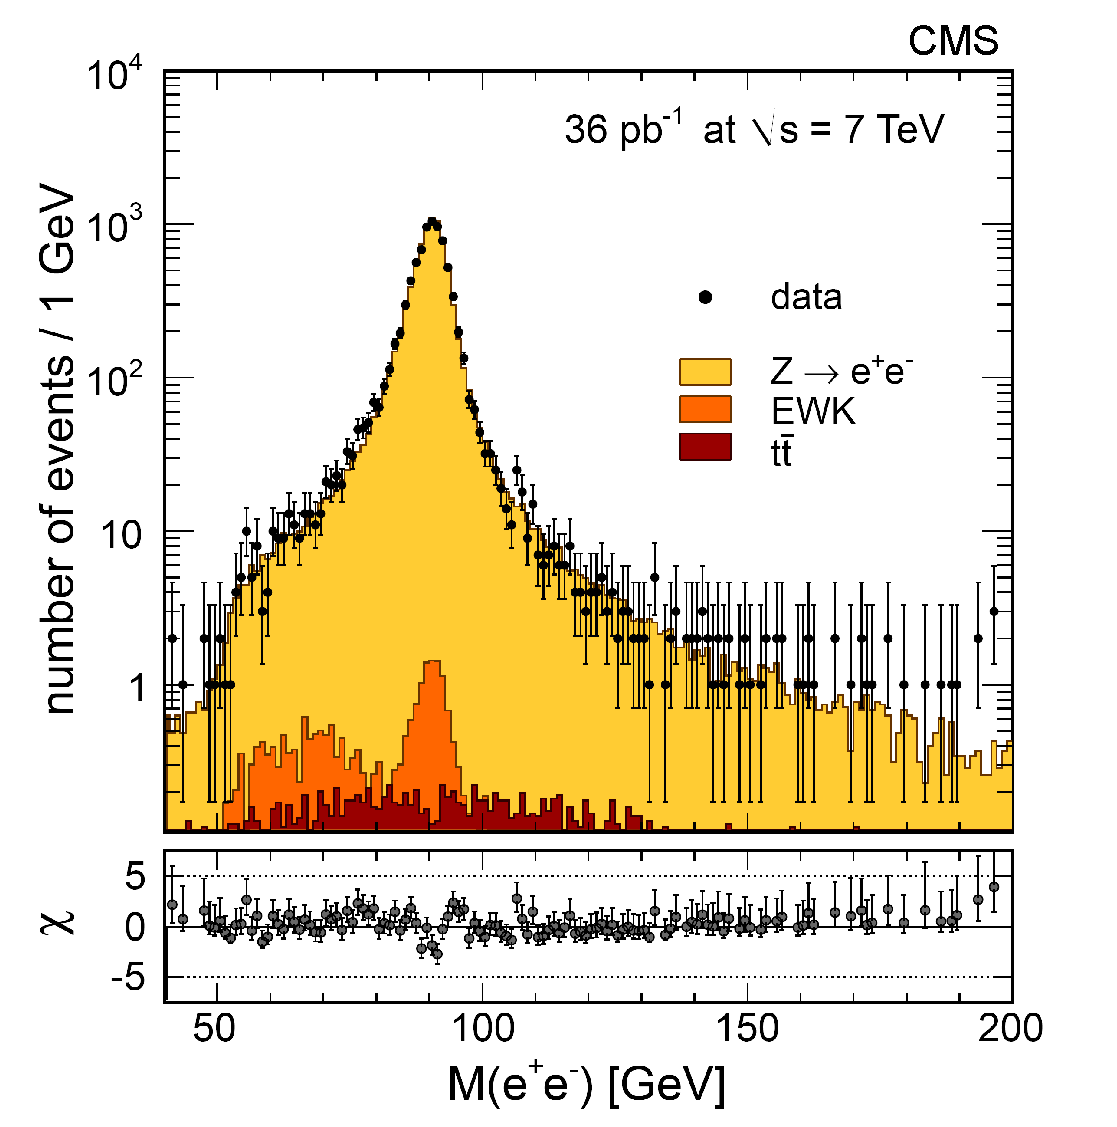
\includegraphics[width=0.48\textwidth]{figs/Zee_mass_Logarithmic_corrected.pdf}
   \caption{ \label{fig:Zee}
Distributions of the dielectron invariant mass for the selected $\Zee$ candidates on
a linear scale (top) and on a logarithmic scale (bottom) before (left)
and after (right) applying energy-scale correction factors.
The points with the error bars represent the data.
Superimposed are the expected distributions from simulations, normalized
to an integrated luminosity of $36$~pb$^{-1}$. The expected distributions are
the Z signal (yellow, light histogram), other EWK processes (orange, medium histogram),
and $\ttbar$ background (red, dark histogram).
Backgrounds are negligible and cannot be seen on the linear-scale plots.
}
  \end{center}
\end{figure}
%%%%%


\subsubsection{Simultaneous Fit}

The $\Zo$ event yield and the electron efficiencies can be extracted from
a simultaneous fit. Two categories of events are
considered: events where both electrons satisfy
the tight selection with $\Et>25\GeV$, and events that consist of
one electron with $\Et>25\GeV$ that passes the tight selection, and one
ECAL cluster with $\Et>25\GeV$ that fails
the selection, either at the reconstruction or electron identification level.

In each category, a signal-plus-background function is fitted to the observed mass spectrum.
The signal shape is taken from signal samples simulated with POWHEG at the NLO generator level,
and is convolved with a Crystal-Ball function modified to include an extra
Gaussian on the high end tail with floating mean and width.
In the first category, the nearly vanishing background is fixed to the
value reported in Table~\ref{tab:ZllBG}. In the second
category of events, the background is modeled by an exponential distribution.

%Fig.~\ref{fig:Zmass_TT_TF} shows the fit to the Tag-Tag events (left plot) and to
%Tag-Fail events (right plot).
The estimated cross section is $988 \pm 10\, \mathrm{(stat.)} \pm 4\mathrm{(syst.)}\,\mathrm{pb}$.
The cross section is in good agreement with the counting analysis estimate of
 $992 \pm 11\, \mathrm{(stat.)}\,\mathrm{pb}$, considering only the statistical uncertainty.
Both techniques give equivalent results. The counting analysis estimate is used for the
cross section measurement in the $\Zee$ channel.

%\begin{figure}
%  \begin{center}
%   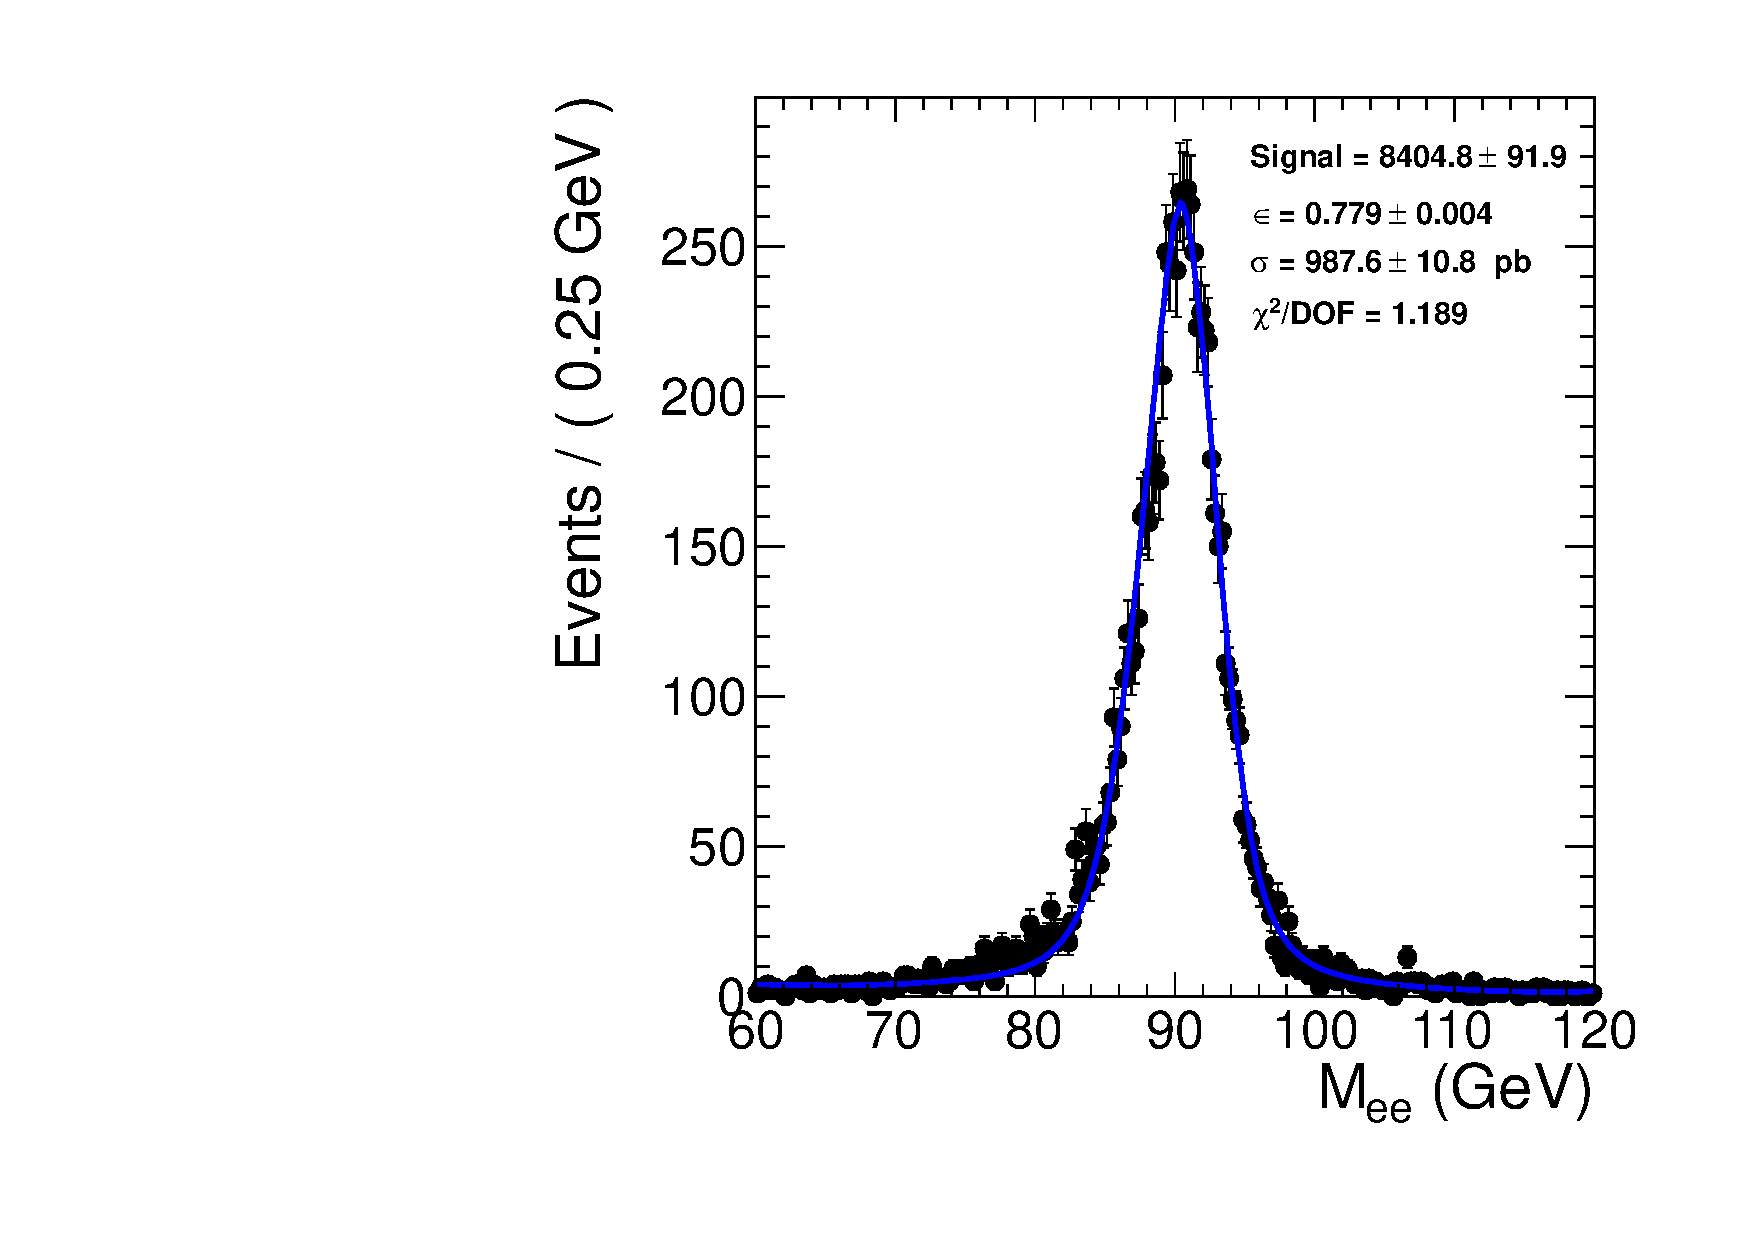
\includegraphics[width=0.48\textwidth]{figs/Zmass_TT_36143nb.pdf}
%   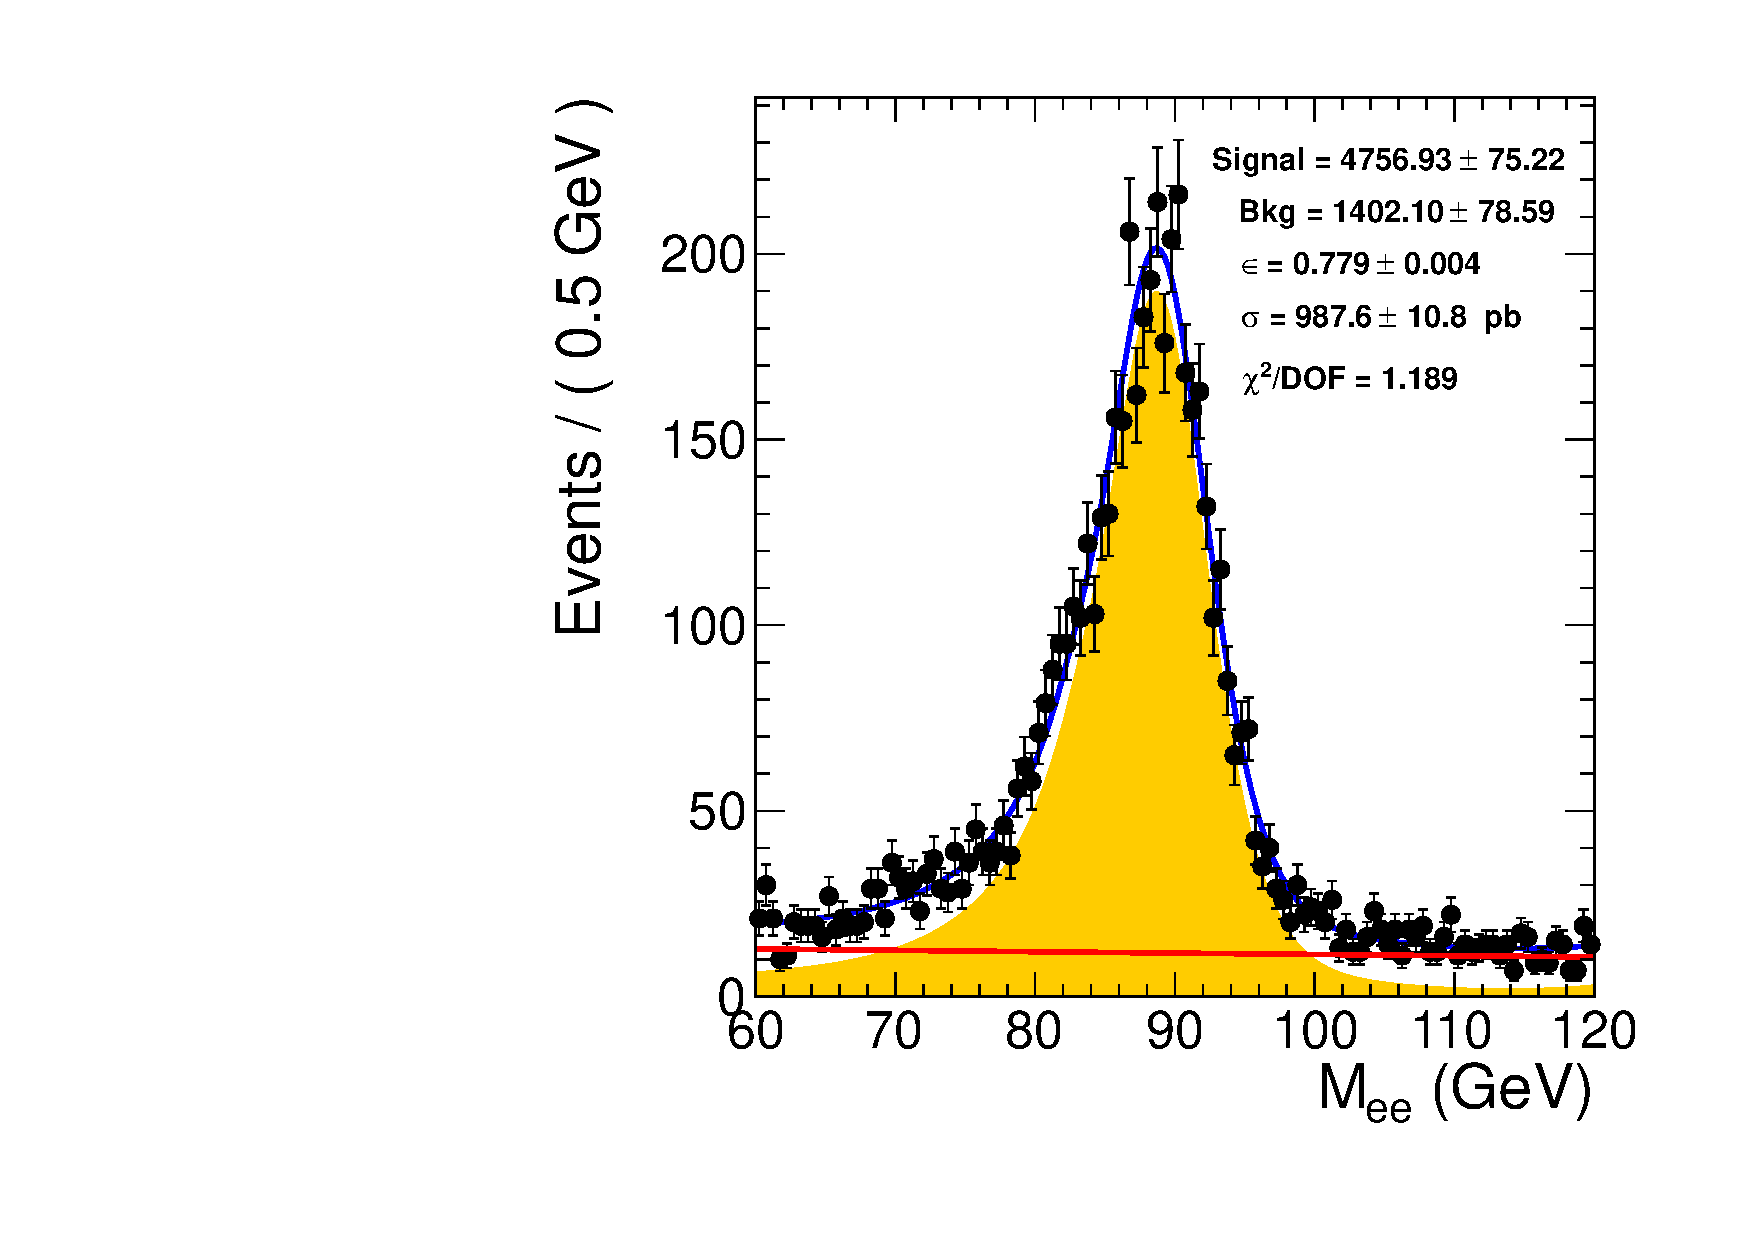
\includegraphics[width=0.48\textwidth]{figs/Zmass_TF_36143nb.pdf}
%   \caption{ \label{fig:Zmass_TT_TF}
%Fits to the Tag-Tag mass distributions (left plot) and Tag-Fail mass distributions (right plot)
%used in the simultaneous determination of the Zee yield and the electron efficiencies. }
%  \end{center}
%\end{figure}

%The electron $p_T$ distribution for $\Zee$ is shown in
%Fig.~\ref{fig:ZpT} in Appendix~\ref{sec:KinDist}.  Also,
%Fig.~\ref{fig:Zkin} shows the dielectron transverse
%momentum ($q_T$) and rapidity ($Y$) distributions.



\subsection{\texorpdfstring{The $\Zmm$ Signal Extraction}{The Z->mu mu Signal Extraction}}
\label{sec:Zmumu}

The yield of the $\Zmm$ events is determined from a fit simultaneously with the
average muon reconstruction efficiencies in the tracker and in
the muon detector, the muon trigger efficiency,
as well as the efficiency of the applied isolation requirement.
\Zmm candidates are obtained as pairs of muon candidates of different types
and organized into categories according to different requirements:
\begin{itemize}
\item $\Zmumu$: a pair of isolated global muons, further split into two samples:
\begin{itemize}
\item $\ZmumuTwoHlt$: each muons associated with an HLT trigger muon;
\item $\ZmumuOneHlt$: only one of the two muons associated with an HLT trigger muon;
\end{itemize}
\item $\Zmus$: one isolated global muon and one isolated
  stand-alone muon;
\item $\Zmut$: one isolated global muon and one isolated tracker track;
\item $\ZmumuNonIso$: a pair of global muons, of which one is isolated and the
other is nonisolated.
\end{itemize}

%The $\Zmumu$ category is also referred to as ``golden'' sample.
With the exception of the $\ZmumuOneHlt$ category, each global muon must correspond to an HLT trigger muon.
The five categories are explicitly forced to be mutually exclusive in the event
selection: if one event falls into the first category it is excluded from the second;
if it does not fall into the first category and falls into the second, it is excluded
from the third, and so on. In this way non-overlapping, hence statistically
independent, event samples are defined. The expected number of events in which more than
one dimuon combination is selected is almost negligible.
In those few cases all possible combinations are considered.

The five signal yields in each category can be written in terms of
the five unknowns, the Z signal yield $\NZtomumu$ and four efficiency terms, as follows:
\begin{eqnarray}
 \label{eqNmumuTwoHlt}
   \NmumuTwoHlt & = & \NZtomumu \effHlt^2 \effIso^2 \effTrk^2 \effSa^2,  \\
  \label{eqNmumuOneHlt}
   \NmumuOneHlt & = & 2 \NZtomumu \effHlt (1 - \effHlt) \effIso^2 \effTrk^2 \effSa^2,  \\
  \label{eqNmus}
   \Nmus & = & 2 \NZtomumu \effHlt \effIso^2 \effTrk (1 - \effTrk) \effSa^2,  \\
  \label{eqNmut}
   \Nmut & = & 2 \NZtomumu \effHlt \effIso^2 \effTrk^2 \effSa(1 -\effSa), \\
  \label{eqNmumuNonIso}
   \NmumuNonIso & = & 2 \NZtomumu \effHlt^2  \effIso (1 - \effIso)  \effTrk^2 \effSa^2.
\end{eqnarray}
The various efficiency terms in Eqs.~(\ref{eqNmumuTwoHlt}) to~(\ref{eqNmumuNonIso}),
the average efficiencies
of muon reconstruction in the tracker, $\effTrk$, in the muon detector as
a stand-alone muon, $\effSa$, the average efficiency of the isolation requirement,
$\effIso$, and the average trigger efficiency, $\effHlt$,
can be factorized because the muon selection
factorizes the requirements on the tracker and muon detector quantities separately.
Neither selection on $\chi^2$ per degree of freedom nor requirement of the muon reconstruction through the
tracker-muon algorithm is applied in order to
avoid efficiency terms that cannot be described as a product of contributions from the tracker and
the muon detector.
%We verified on Monte Carlo that the possible effects of any residual correlation
%can be either incorporated in the proper definition of the efficiencies or
%is negligible.
% Above, $\effTrk$ is
% the efficiency to reconstruct a track {\it and} to pass the track selection,
% and $\effSa$ is the efficiency to reconstruct a track in the muon detector {\it and} to pass the
% stand-alone muon selection, according to the selection described in Section~\ref{sec:muonid}.

The dimuon invariant mass spectra for the five categories are divided into
bins of different sizes, depending on the number of observed events.
The distributions of the dimuon invariant mass for the different categories can be written
as the sum of a signal peak plus a background component.


Figure~\ref{fig:zGolden36pb} shows the dimuon invariant mass spectrum for the $\Zmm$ golden events
on both a linear scale and a logarithmic scale, and Figs.~\ref{fig:zNoGold1}
and~\ref{fig:zNoGold2} show the
invariant mass distributions for the remaining categories.
The spectra are in agreement with the simulation.

\begin{figure}[hbtp]
    \begin{minipage}{73mm}
      \begin{center}
%        \resizebox{1.0\textwidth}{!}{{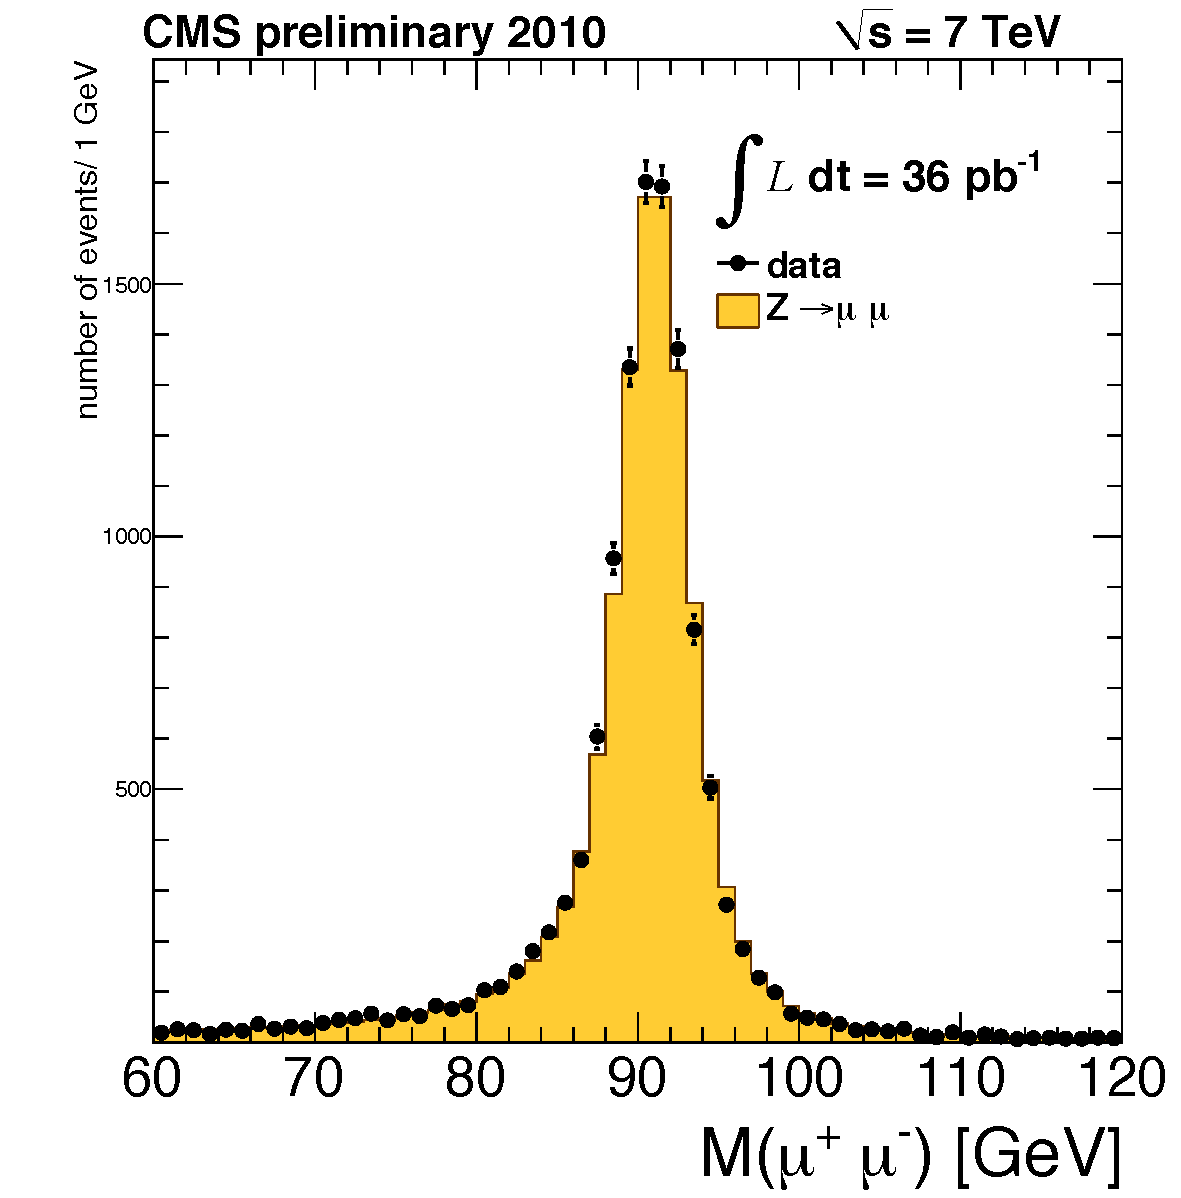
\includegraphics{figs/zGoldenLin_36pb.pdf}}}
        \resizebox{1.0\textwidth}{!}{{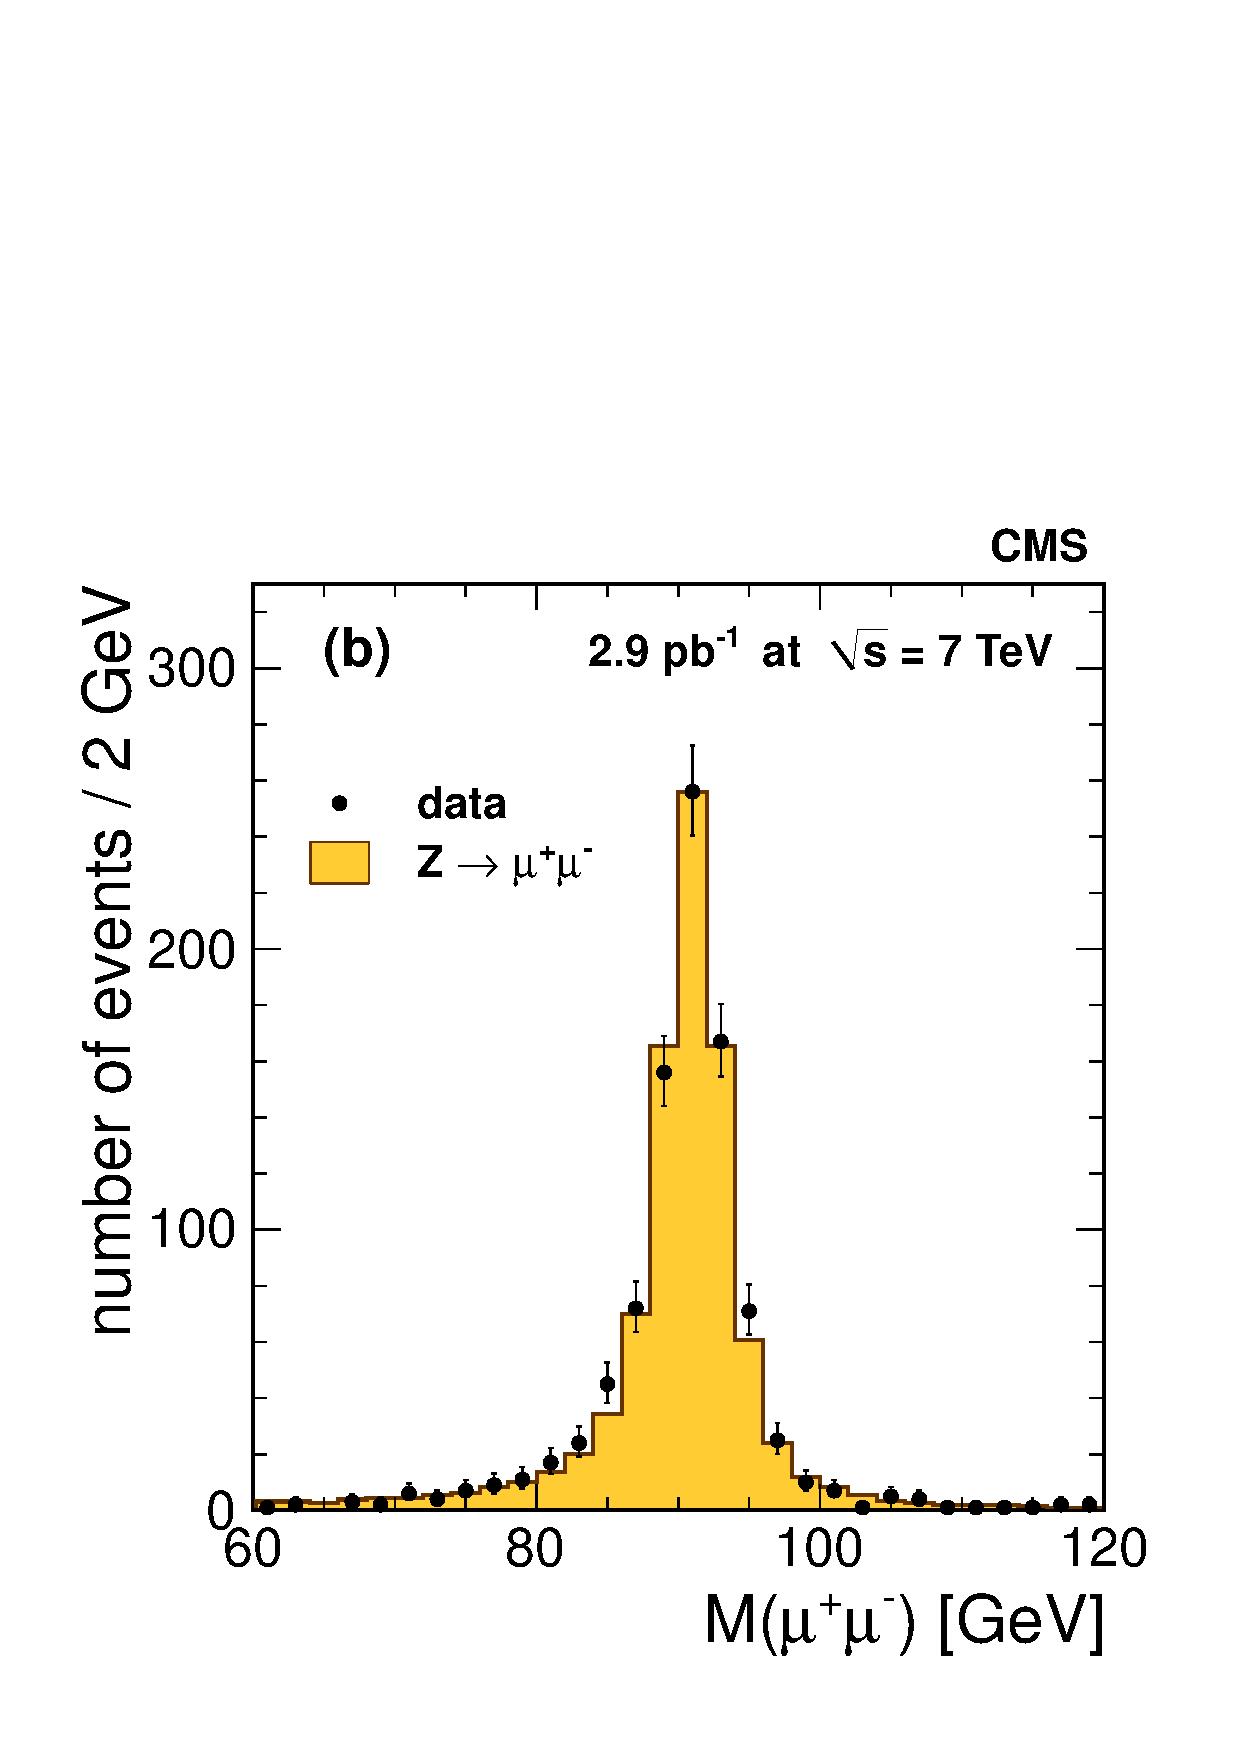
\includegraphics{figs/Zmumu_lin.pdf}}}
      \end{center}
    \end{minipage}
    \begin{minipage}{73mm}
       \begin{center}
%       \resizebox{!}{1.0\textwidth}{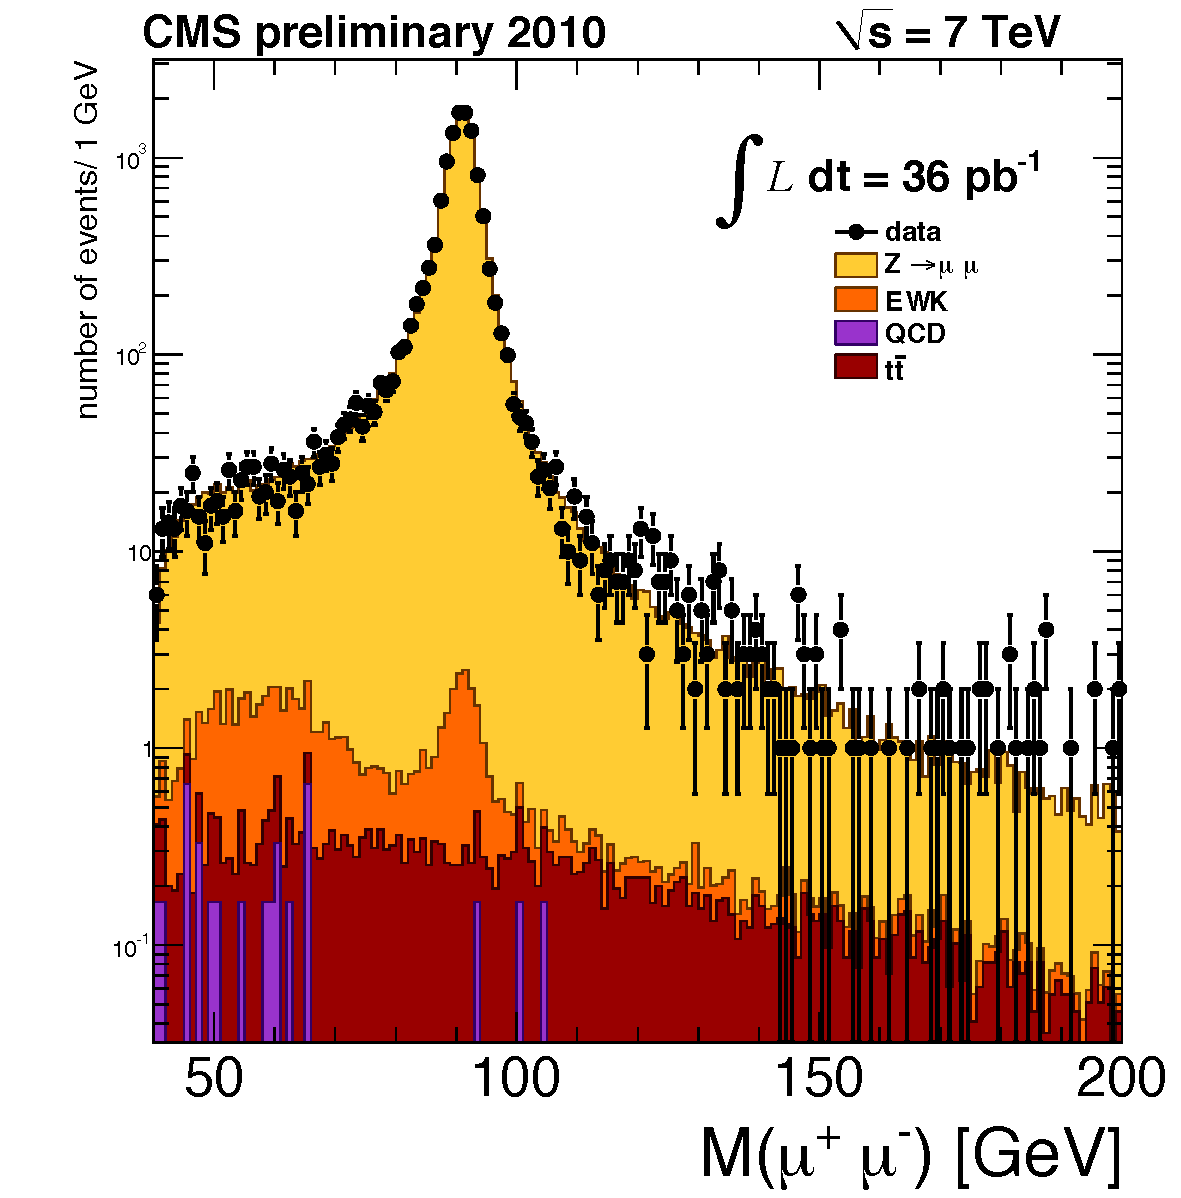
\includegraphics{figs/zGoldenLog_36pb.pdf}}
       \resizebox{!}{1.0\textwidth}{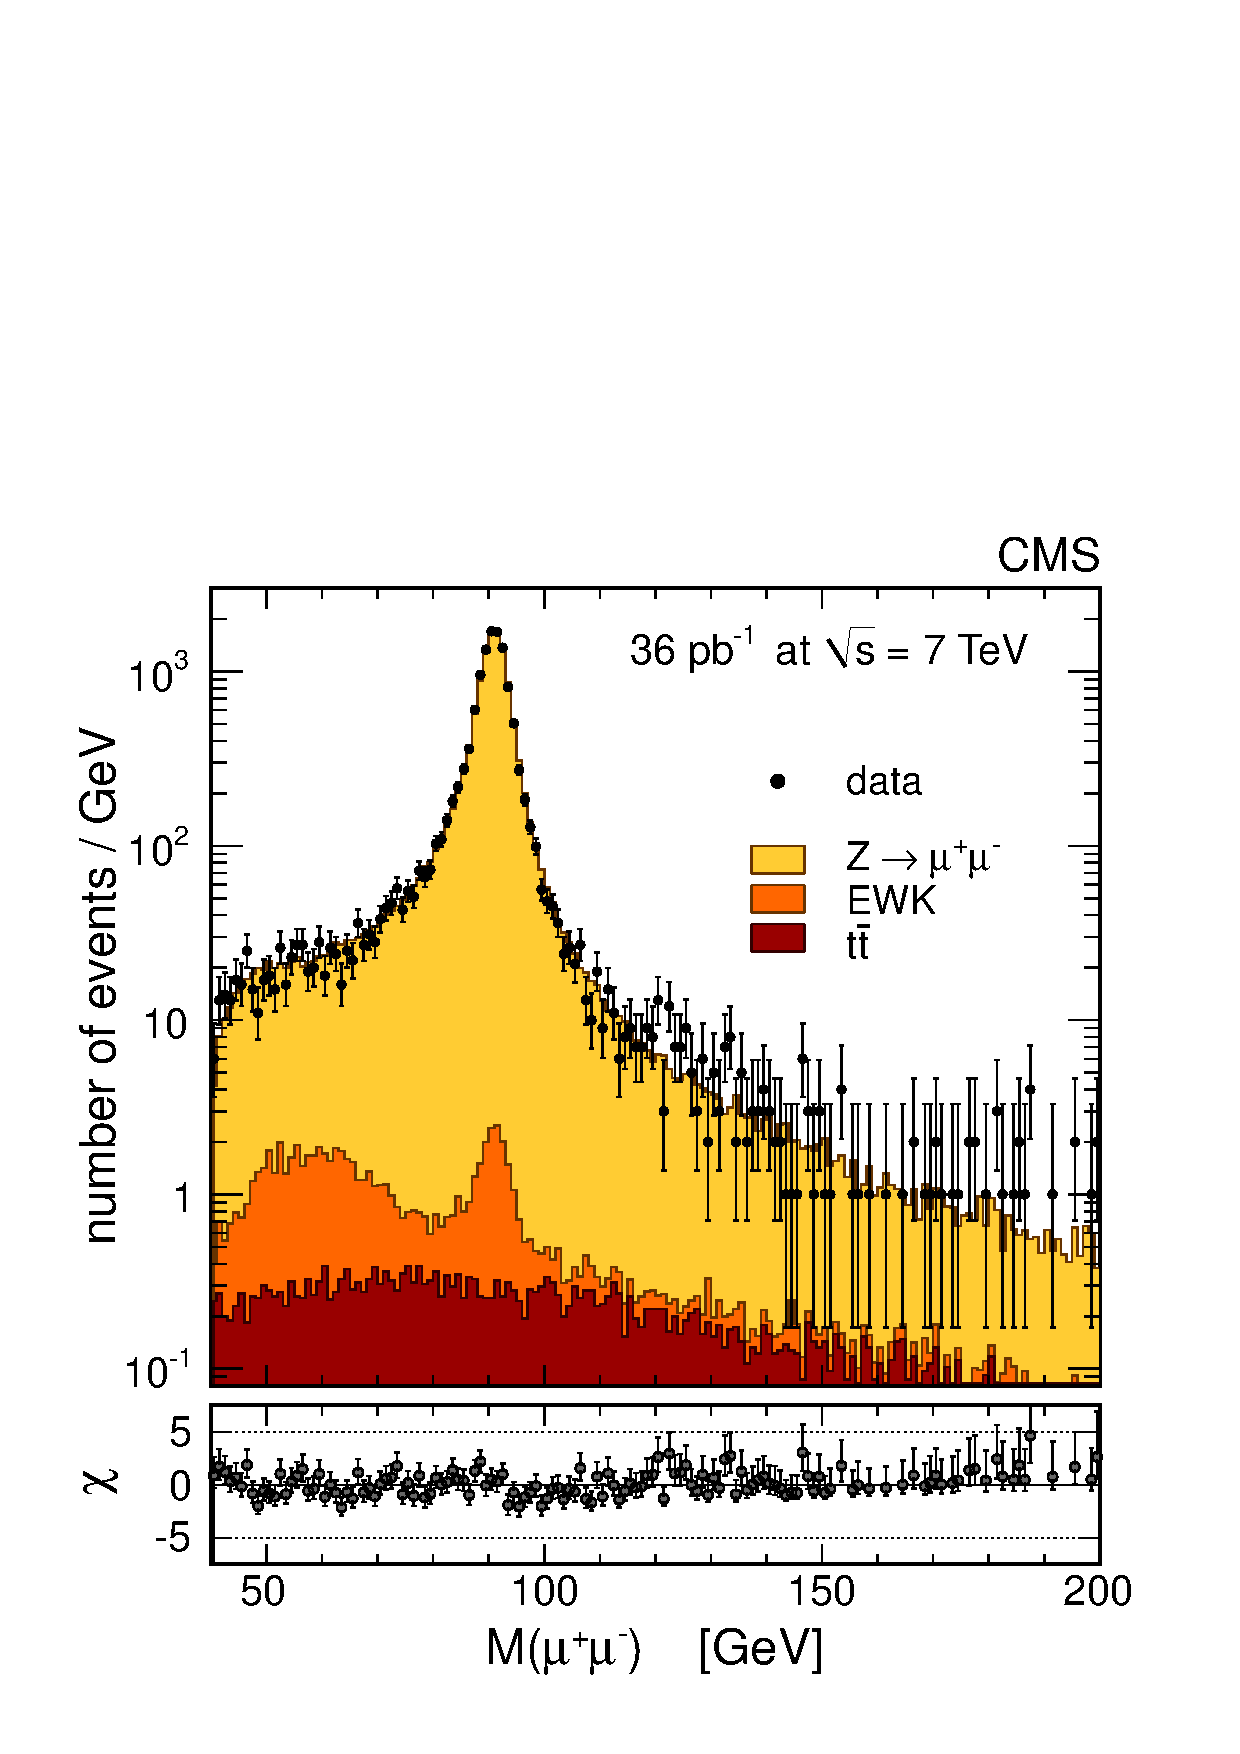
\includegraphics{figs/Zmumu_log.pdf}}
      \end{center}
    \end{minipage}
\caption{
Distributions of the dimuon invariant mass for the selected $\Zmm$ golden candidates on
a linear scale (left) and on a logarithmic scale (right).
The points with the error bars represent the data.
Superimposed are the expected distributions from simulations, normalized
to an integrated luminosity of $36$~pb$^{-1}$. The expected distributions are
the Z signal (yellow, light histogram), other EWK processes (orange, medium histogram),
and $\ttbar$ background (red, dark histogram).
Backgrounds are negligible and cannot be seen on the linear-scale plots.
}
\label{fig:zGolden36pb}
\end{figure}

\begin{figure}[hbtp]
    \begin{minipage}{73mm}
      \begin{center}
        \resizebox{1.0\textwidth}{!}{{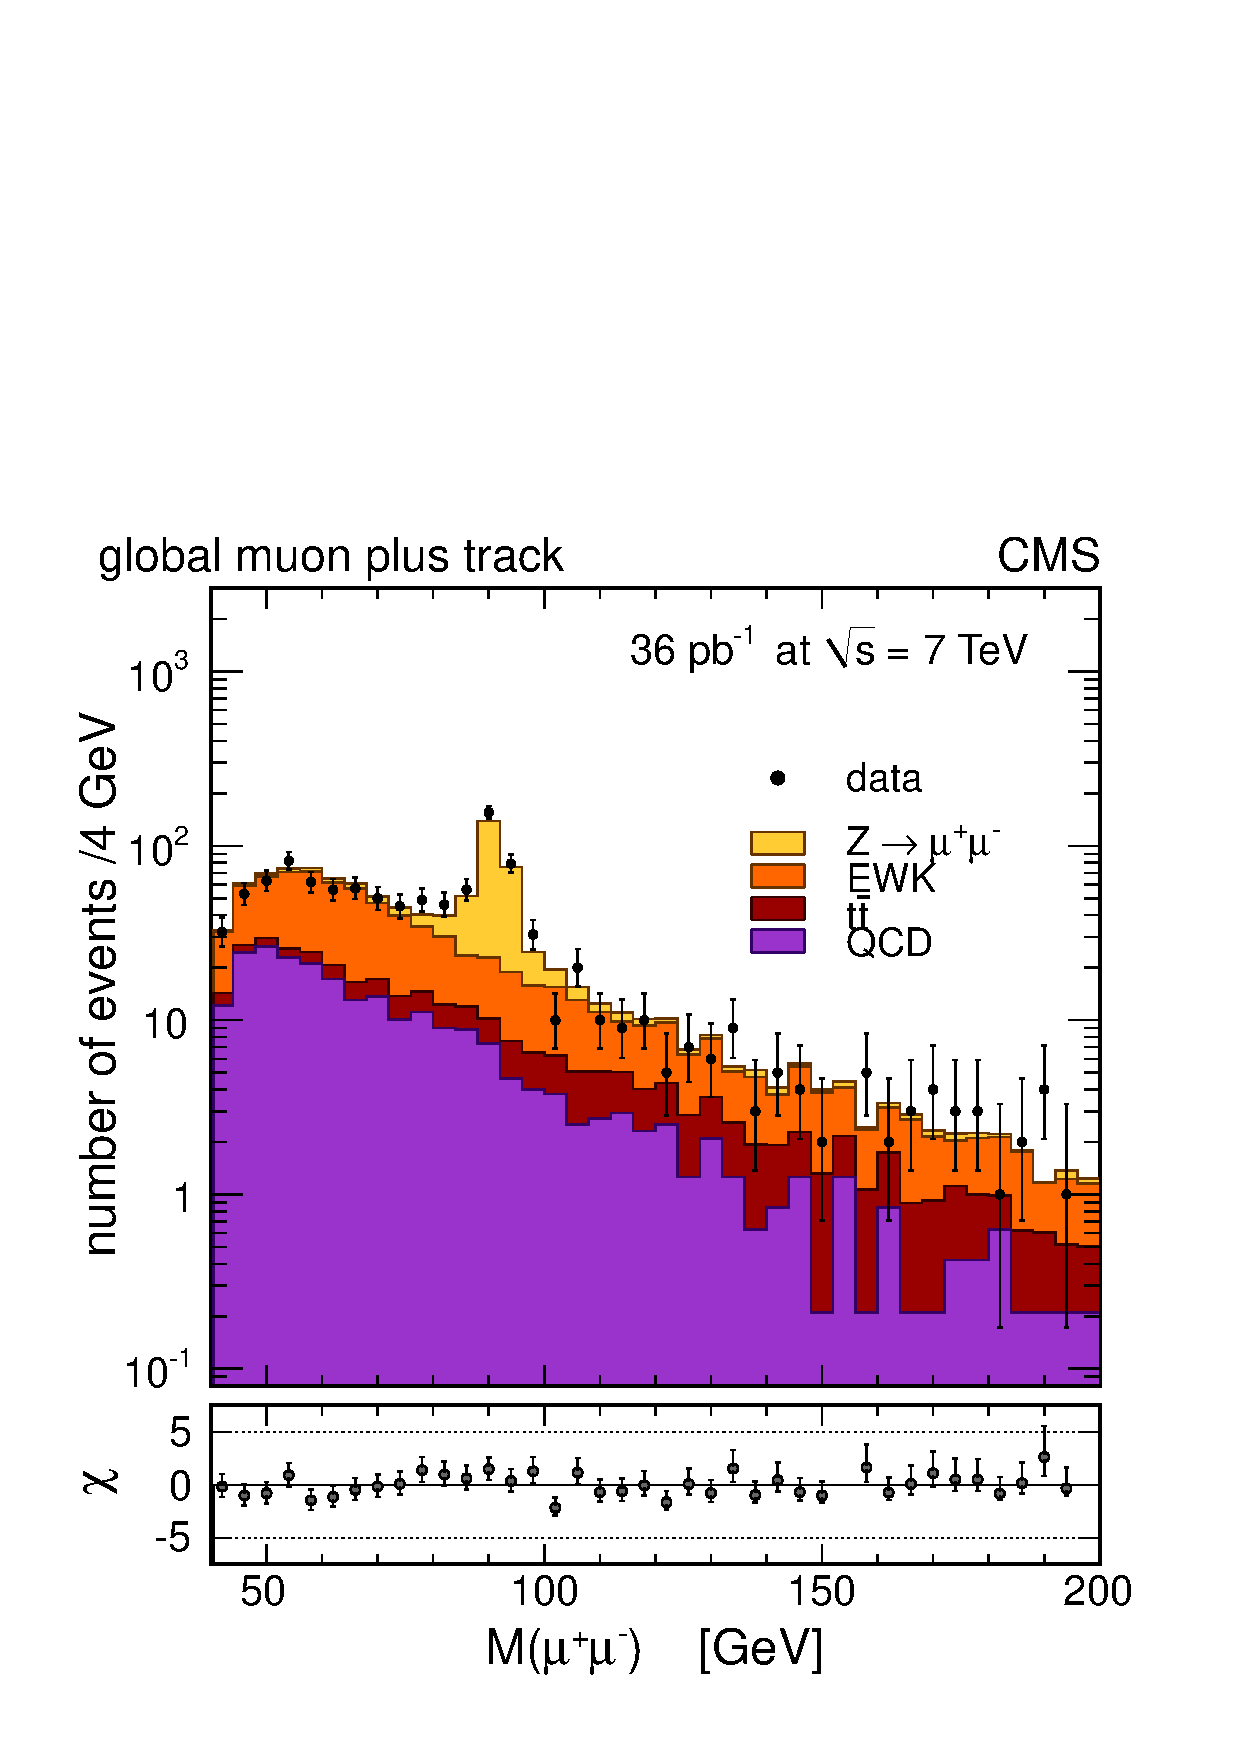
\includegraphics{figs/ZMuTrk_log.pdf}}}
      \end{center}
    \end{minipage}
    \begin{minipage}{73mm}
       \begin{center}
       \resizebox{!}{1.0\textwidth}{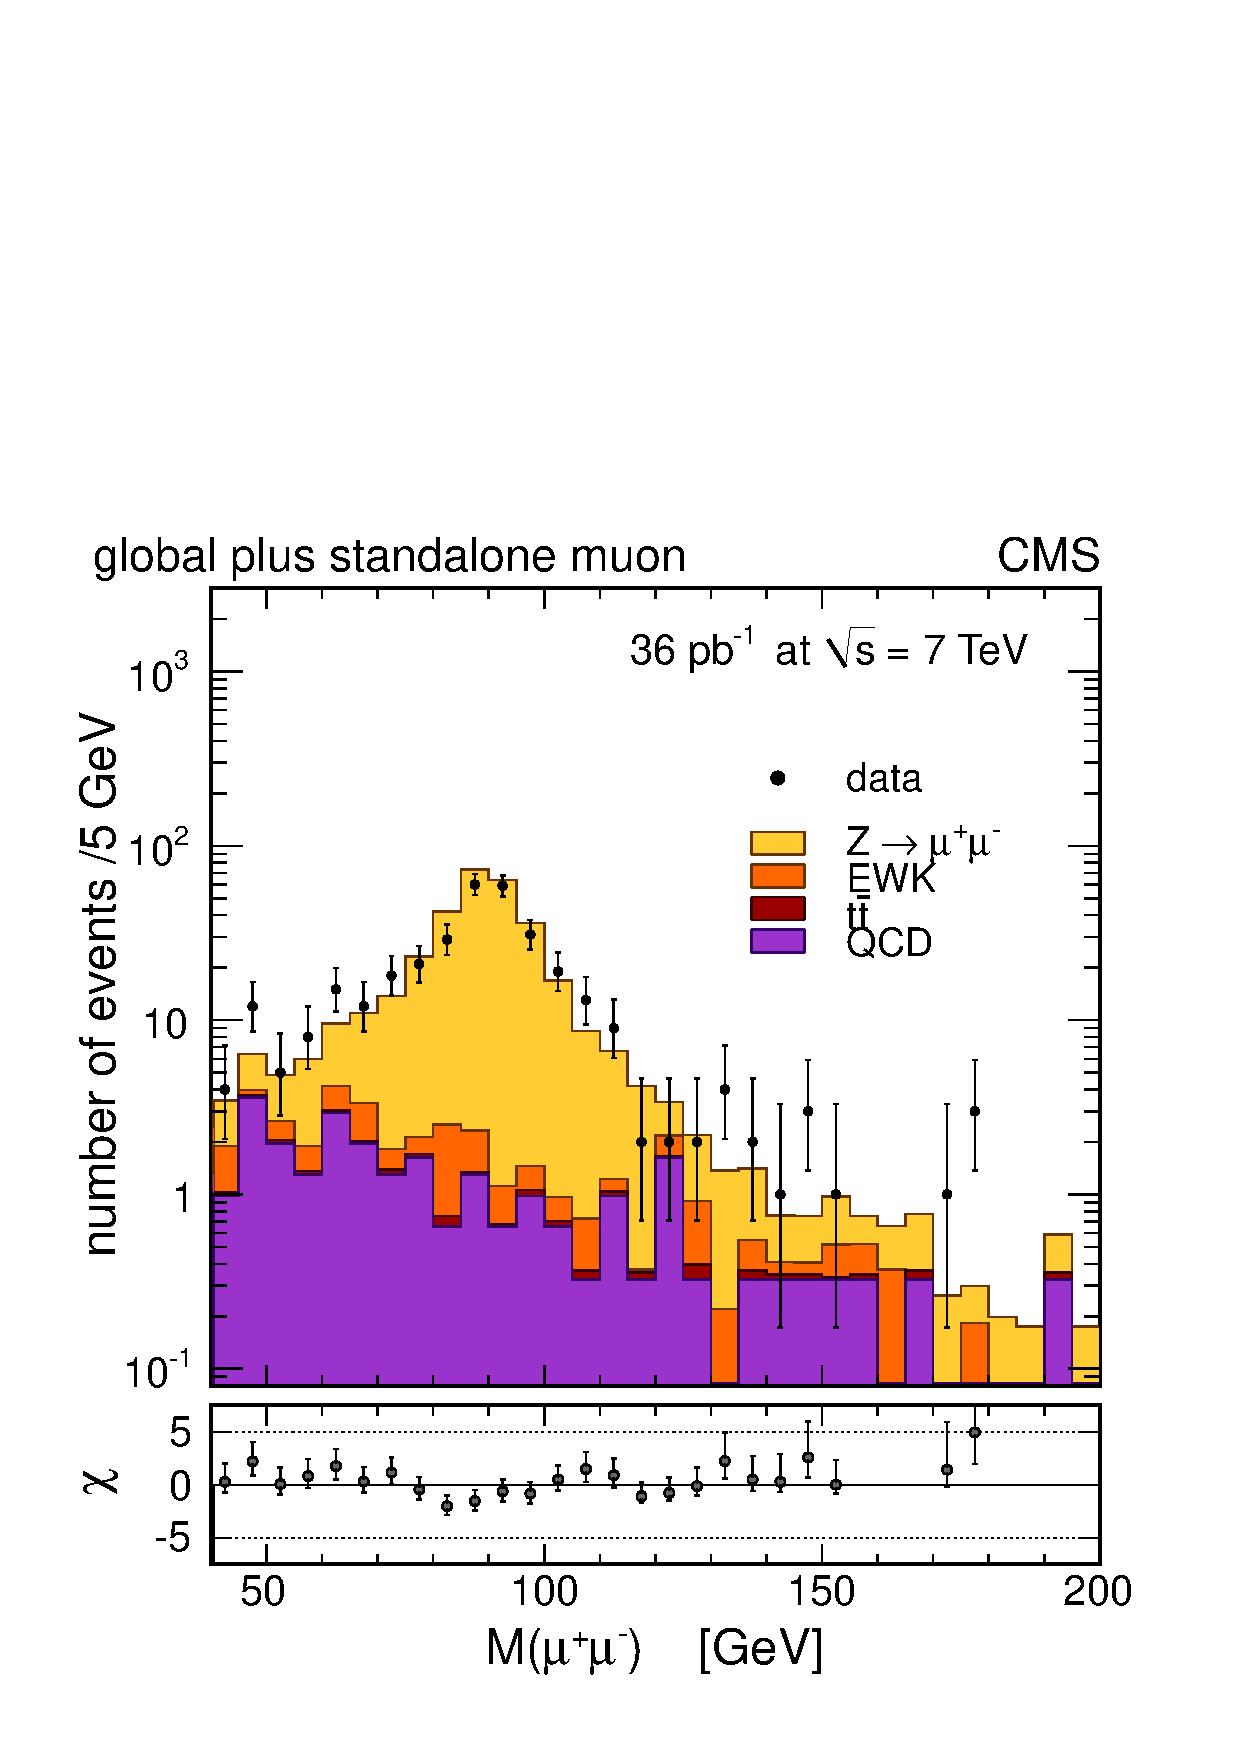
\includegraphics{figs/ZMuSta_log.pdf}}
      \end{center}
    \end{minipage}
\caption{Distributions of the dimuon invariant mass for the selected
$\Zmut$ (left) and $\Zmus$ (right) candidates.
The points with the error bars represent the data.
Superimposed are the expected distributions from simulations, normalized
to an integrated luminosity of $36$~pb$^{-1}$. The expected distributions are
the Z signal (yellow, light histogram), other EWK processes (orange, medium histogram),
$\ttbar$ background (red, dark histogram) and QCD background (violet, black histogram).
}
\label{fig:zNoGold1}
\end{figure}
\begin{figure}[hbtp]
    \begin{center}
     \begin{minipage}{73mm}
       \begin{center}
        \resizebox{!}{1.0\textwidth}{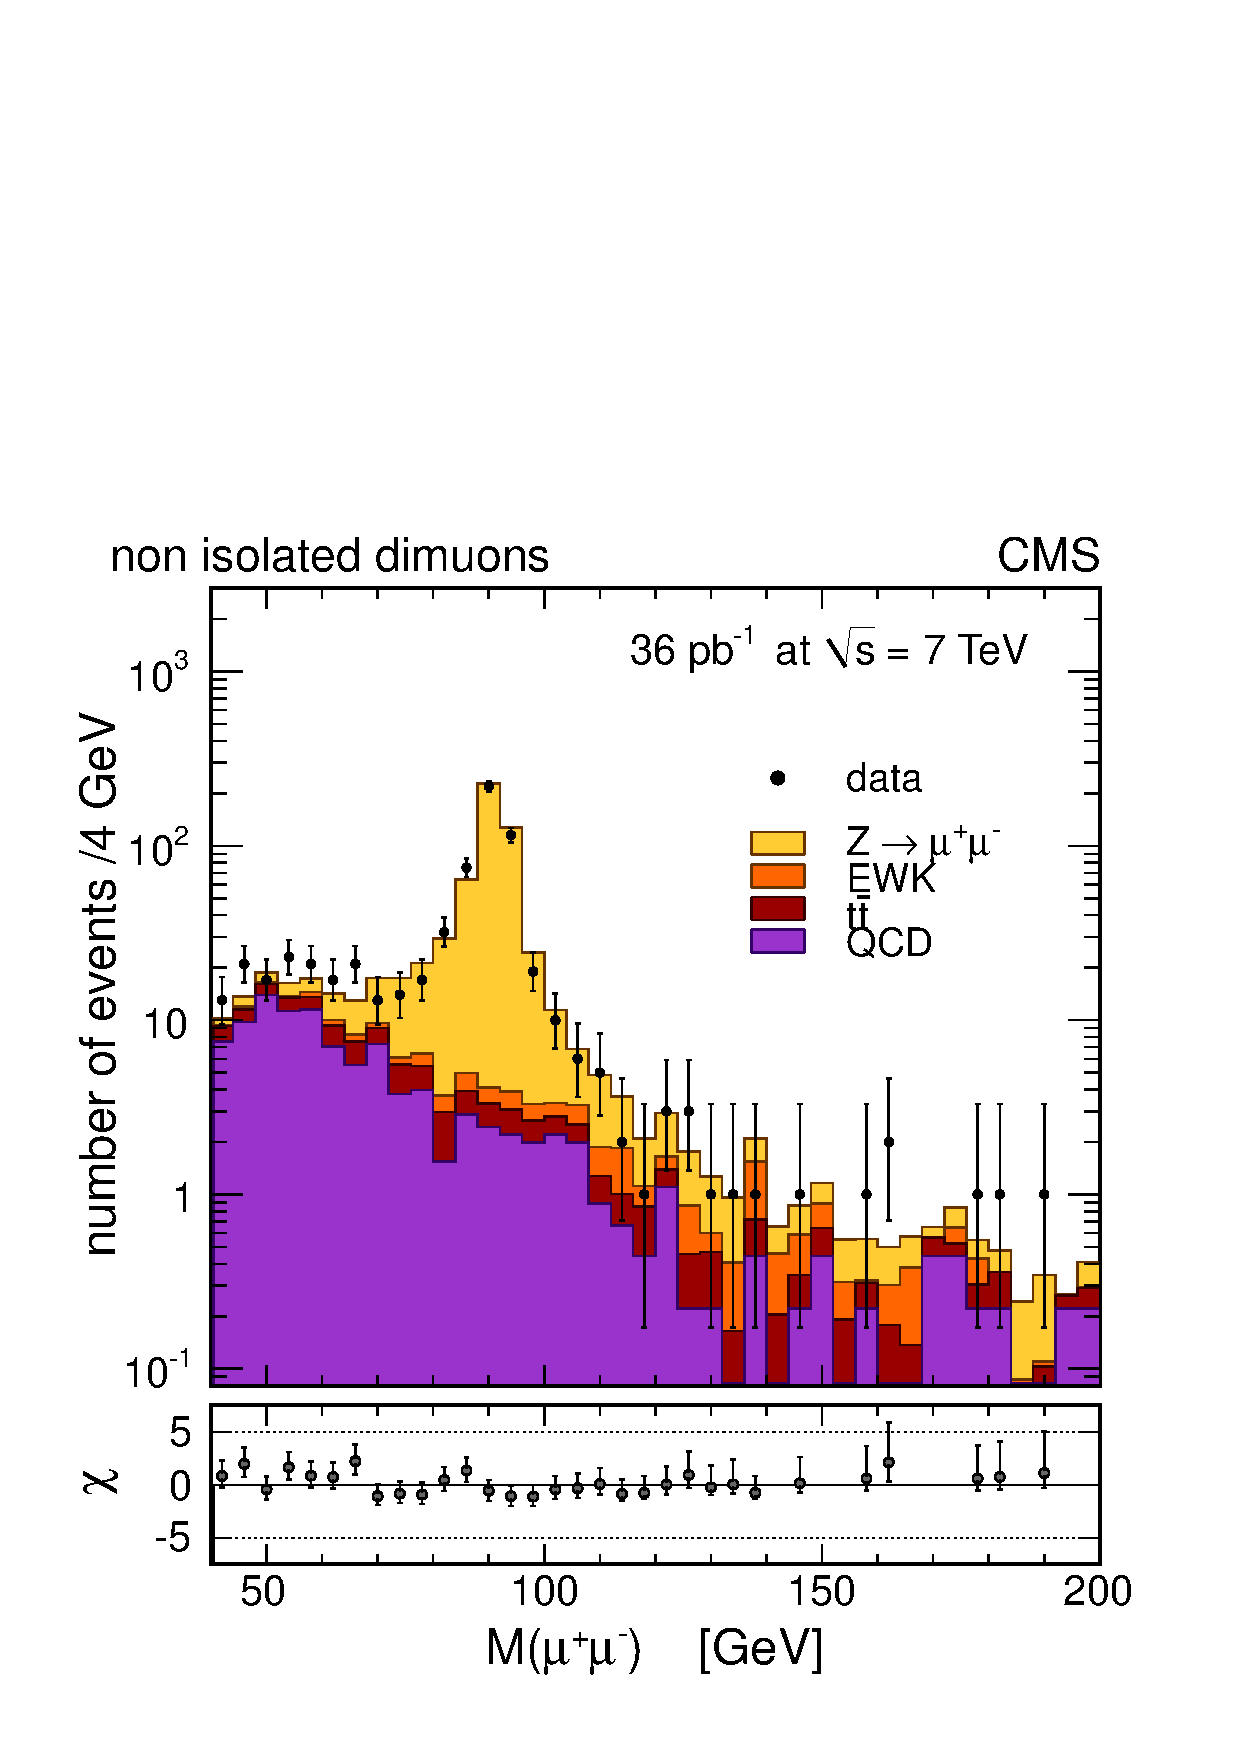
\includegraphics{figs/ZNotIso_log.pdf}}
       \end{center}
     \end{minipage}
   \end{center}
\caption{Distributions of the dimuon invariant mass for the selected
$\ZmumuNonIso$ candidates.
The points with the error bars represent the data.
Superimposed are the expected distributions from simulations, normalized
to an integrated luminosity of $36$~pb$^{-1}$. The expected distributions are
the Z signal (yellow, light histogram), other EWK processes (orange, medium histogram),
$\ttbar$ background (red, dark histogram), and QCD background (violet, black histogram).
}
\label{fig:zNoGold2}
\end{figure}

%, and the background can be considered
%negligible in the 'golden' categories (of the order of few per mille).
% \begin{eqnarray}
%    \NmumuTwoHlt (m) & = & \NmumuTwoHlt f_{peak}(m)\,, \\
%    \NmumuOneHlt (m) & = & \NmumuOneHlt f_{peak}(m)\,, \\
%    \Nmus (m) & = & \Nmus f^s_{peak}(m) + b_{\mu s}(m)\,, \\
%    \Nmut (m) & = & \Nmut f_{peak}(m) + b_{\mu t}(m)\,, \\
%    \NmumuNonIso (m) & = & \NmumuNonIso f_{peak}(m) + b_{\mu\mu}^{\mathrm{non\,iso}}(m)\,. \\
% \end{eqnarray}
The signal-peak distribution can be considered to be identical in the categories
$\Zmumu$ and $\Zmut$  because the momentum resolution in CMS is determined predominantly
by the tracker measurement for muons with $\Pt \leq 200$ GeV.
The binned spectrum of the dimuon invariant mass in the
$\Zmumu$ category, which has the most events of all categories,
is taken as shape model for all categories but $\Zmus$.
The large size of the golden sample ensures that the statistical
uncertainty of the invariant mass distribution has a negligible effect on the cross
section measurement.
The small presence of background is neglected in this distribution.
The uncertainty due to this approximation has been evaluated and
taken as the systematic uncertainty as described in Section~\ref{sec:muonSyst}.

Because only tracker isolation is used, the shape obtained from golden events
can also be used to model the $\ZmumuNonIso$ peak distribution.
A requirement on calorimetric isolation would have distorted the dimuon invariant mass
distribution of events with one nonisolated muon because of FSR,
as has been observed both in simulation and data.

The model of the invariant mass shape for the $\Zmus$ category is also derived from golden dimuon events.
The three-momentum for one of the two muons is taken from only the muon detector track fit,
in order to emulate a stand-alone muon.
To avoid using the same event twice in forming the $\Zmus$ shape model,
the higher-$\Pt$ (lower-$\Pt$) muon is chosen for even (odd) event numbers.

Background shapes are modeled as products of an exponential times a polynomial
whose degree depends on the category.
% :
% \begin{eqnarray}
%   b_{\mu t}(m) & = & N^b_{\mu t} (1 + a_1 m + a_2 m^2) e^{-\alpha m} \\
%   b_{\mu\mu}^{\mathrm{non\,iso}}(m) & = &
%   N_{\mu\mu}^{b\,\,{\mathrm{non\,iso}}} (1 + b_1 m + b_2 m^2) e^{-\beta m} \\
%   b_{\mu s}(m) & = & N^b_{\mu s} (1 + c_1 m + c_2 m^2) e^{-\gamma m}
% \end{eqnarray}
Different background models and different binning sizes are considered for the
categories other than $\Zmumu$ and a systematic uncertainty related to the fitting
procedure is determined accordingly.

%  f_{peak}^{s}(m) & = & \frac{1}{\sqrt{2\pi\sigma_s^2}} e^{-\frac{(m - M)^2}{2 \sigma_s^2} } \\
%The peak function for the $\Zmus$ category, $f_{peak}^{s}(m)$, is modeled as a
%Gaussian, due to the poor resolution, and the low statistics in that sample:

A simultaneous binned fit based on a Poissonian likelihood~\cite{PoisLR} is performed
for the different categories.
%We define, for each category, minus two times the negative logarithmic
%of the following Poissonian likelihood ratio~\cite{PoisLR}:
% \begin{equation}
% \chi^2_{\lambda} = -2 \ln{\lambda(m)} =  -2 \ln{\frac{\mathrm{Poiss}(n_i,
%     \nu_i)}{\mathrm{Poiss}(n_i, n_i)}} = \sum_{i=1}^{n_{\mathrm{bins}}} \nu_i - n_{i} + n_i \log{\frac{n_i}{\nu_i}}\,,
% \end{equation}
% where $\nu_i$ is the expected number of events in the $i^{\mathrm{th}}$-bin in $m$,
% $n_i$ is the measured number of events in that
% bin, and $\mathrm{Poiss}(n,\nu)$ is a Poissonian distribution.
% The simultaneous fit is performed minimizing the sum $R$ of the five $\chi^2_\lambda,j$ from
% the different categories $j=1,\cdots, 5$, i.e.:
% \begin{equation}
% R =  \sum_{j=1}^{5} \chi^2_{\lambda,j}   = 2  \sum_{j=1}^{5} \sum_{i=1}^{n_{\mathrm{bins}}^{(j)}} \nu^{(j)}_i - n^{(j)}_{i} + n^{(j)}_i \log{\frac{n^{(j)}_i}{\nu^{(j)}_i}}\,.
% \label{eq:PoisLR}
% \end{equation}
% For sufficiently large $\nu_i$, as in our case, the minimum of $R$ follows with good approximation a $\chi^2$ distribution,
% allowing a goodness-of-fit test.
% Using only the number of events for the two categories with the largest statistics,
% $\ZmumuTwoHlt$ and $\ZmumuOneHlt$, the Z yield and the four efficiencies can be obtained minimizing the
% following expression, which can be obtained from Eq.~\ref{eq:PoisLR} using a single bin in the Gaussian approximation for $\ZmumuTwoHlt$
% and $\ZmumuOneHlt$:
% \begin{eqnarray*} \label{chi2}
% R & = &
% \frac{(\NmumuTwoHlt - \NZtomumu\effHlt^2\effIso^2\effTrk^2\effSa^2)^2}{\NmumuTwoHlt} +  \\
% & & \frac{(\NmumuOneHlt - 2\NZtomumu\effHlt(1-\effHlt)\effIso^2\effTrk^2\effSa^2)^2}{\NmumuOneHlt} +  \\
% & & \chi^2_{\lambda, \mu s} +
% \chi^2_{\lambda, \mu t} +
% \chi^{\nonIso\,\, 2}_{\lambda, \mumu}\, ,
% \end{eqnarray*}
% where we use the event counts only in the  $\ZmumuOneHlt$ and $\ZmumuTwoHlt$ 'golden'
% categories and the Poissonial terms $\chi^2_{\lambda, \mu s}$, $\chi^2_{\lambda, \mu t}$ and
% $\chi^{\nonIso\,\, 2}_{\lambda, , \mumu}$ for the remaining categories.
% The likelihood ratio fit is equivalent to an ordinary $\chi^2$
% for sufficiently large statistics and we verified that, with the current data sample,
% it gives the same central value and statistical uncertainty.
%We perform the fit in the range $60 < m < 120~\mathrm{GeV}/c^2$.
%Full details on the signal and background modeling assumptions and
%correlation studies are present in~\cite{CMS_AN_2010-345}.
Table~\ref{fig:fitRes_36pb} reports the signal yield and single-muon efficiencies determined from
the simultaneous fit and the ratios of the fitted to simulation efficiencies.
A goodness-of-fit test gives a probability ($p$-value) of 0.36 for this fit.

%The resulting fit $p$-value shows the good quality of the fit.
%With the analyzed statistics, a second degree polynomial function is
%taken for modeling  the background shape.

\begin{table}[htbp] %L.L.
\begin{center}
\caption{Signal yield and efficiencies determined from data with the simultaneous fit, and
  ratios of efficiencies determined from the fit and the simulation.}
\label{fig:fitRes_36pb}
\begin{tabular}{|c|c|c|}
\hline
Quantity & Fit results from data & Data/simulation\\
\hline\hline
$\NZtomumu$ &13\,728 $\pm$ 121   & \\
\hline
$\effHlt$ & 0.9203 $\pm$ 0.0019  &0.9672 $\pm$ 0.0020   \\
$\effIso$ & 0.9813 $\pm$ 0.0010& 0.9962 $\pm$  0.0011 \\
$\effSa$ & 0.9762  $\pm$ 0.0012 & 0.9964 $\pm$ 0.0013 \\
$\effTrk$ & 0.9890 $\pm$ 0.0006  & 0.9949 $\pm$ 0.0007  \\
\hline
\end{tabular}
\end{center}
\end{table}

%In order to correct the fitted yield $\NZtomumu$ for the presence of background,
%the estimated irreducible background fraction is subtracted.
%$f_{bkg}=0.44 \pm 0.02\%$.

The background in the $\Zmumu$ golden category (of the order of few per mille)
was neglected in the fit. In order to correct the fitted yield $\NZtomumu$ for
the presence of this background, we subtract the small estimated irreducible
background fraction.

A $(1.0\pm 0.5)\%$ overall efficiency correction due to the loss of muon events because of trigger
prefiring is also applied (Section~\ref{sec:muonEff}).

The estimated cross section is $968\pm 8 \mathrm{(stat.)}$~pb.

As cross-check, a simpler analysis based on event counting was also performed.
The same selection was applied, and the number of events with two global muon, reported
in Sec~\ref{sec:muonid}, was used as signal yield. 
The signal yield was then corrected for the relevant efficiencies that have 
been evaluated with a \TNP method in a single $\Pt$ and $\eta$ bin, resulting in a
cross section estimate of $969\pm 8 \mathrm{(stat.)}$~pb, in good agreement
with the simultaneous fit method.

\section{Systematic uncertainties}
\label{sec:syst}
We consider several sources of systematic uncertainty, taking into
account their effect on both the signal acceptance and on the template
shapes for the signal extraction fit.  The uncertainty on the
normalization of the backgrounds is taken as part of the statistical
uncertainty.  The largest source of systematic uncertainty is the
shape uncertainty of the W+jets template.  Other sources of systematic
uncertainty considered include jet energy scale (JES) as well as
trigger and lepton identification efficiencies.
%%%%%%%%%%%%%%%%%%%%%%%%%%%%%%%%%%%%%%%%%%%%
\subsection{Systematics due to the W+jets shape}
\label{sec:syst_mjj}
%%%%%%%%%%%%%%%%%%%%%%%%%%%%%%%%%%%%%%%%%%%%%
The $m_{jj}$ shape for W+jets events is taken from the MC.  Its shape
could be different due to NLO corrections and other effects.
Figure~\ref{fig:wjetshapes} shows possible shapes derived from our MC
samples.  To evaluate the effect of these shapes and propagate them
into our limit, we use the five MadGraph samples, which are the large
statistics nominal sample, one sample with the $q^2$ factorization and
renormalization scale doubled, one with the $q^2$ scale halved, one
with the matching scale doubled and one with the matching scale
halved.  We find an ``optimal'' mixture of the MC samples during our
nominal fit and its uncertainty is propagated by the fitter into the
yields and thus into our final limit. %the technique described in
%Section~\ref{sec:wjetsShape} separately for the 2- and 3-jet bins.
%The shapes that are produced corresponding to the different systematic
%variations on the parameters are propagated to the limit setting as a
%systematic error.

%\subsubsection{Uncertainty due to limited amount of MC}
%The main source of systematic error on the W+jets shape is due to the limited amount of MC
%events in the samples. We evaluate this error by producing Toy MC $m_{jj}$ templates
%based on those from the centrally produced sample. The toy templates are passed through the 
%same optimization procedure and a new optimal mixture is obtained. The resulting uncertainty
%on the W$jj$(Diboson) yield is $XX$($XX$) events for the 2-jet bin and $XX$($XX$) events for 
%the $3$-jet bin.
%Using the distributions of the 
%parameters of the mixture we can evaluate the error on those parameters 
%and propagate that error to the limit setting machinery.

%\subsubsection{Uncertainty due to Factorization Scale and ME-PS Matching}
%The fractions of $q^2$ and matching samples in the overall
%(``optimal'') mixture, obtained from the optimization procedure, have
%corresponding uncertainties.  In order to take the $q^2$-matching
%correlations into account it is necessary to perform a scan in both
%dimensions. Specifically, we vary the scaling and matching fractions
%within $\pm 0.2$ of the optimal values. The systematic error on the
%W$jj$ yield is the difference between the value at the minimum
%-loglikelihood ($nll_{Min}$) and the value at $nll_{Min}+1/2$.
%We scan the $nll_{Min}+1/2$ contour and take the largest difference
%(between the W$jj$ yield at the minimum and on the contour) to be the
%systematic error. The scan results are shown in
%Figs.~\ref{fig:NLL2DScan_2j},~\ref{fig:NLL2DScan_3j}.  The error on
%the W$jj$ yield is 153 events (174 events) in the 2-jet (3-jet) bin.
%%%%%%%%%%%%%%%%%%%%%
%\begin{figure}[htb] 
%  {\centering
%    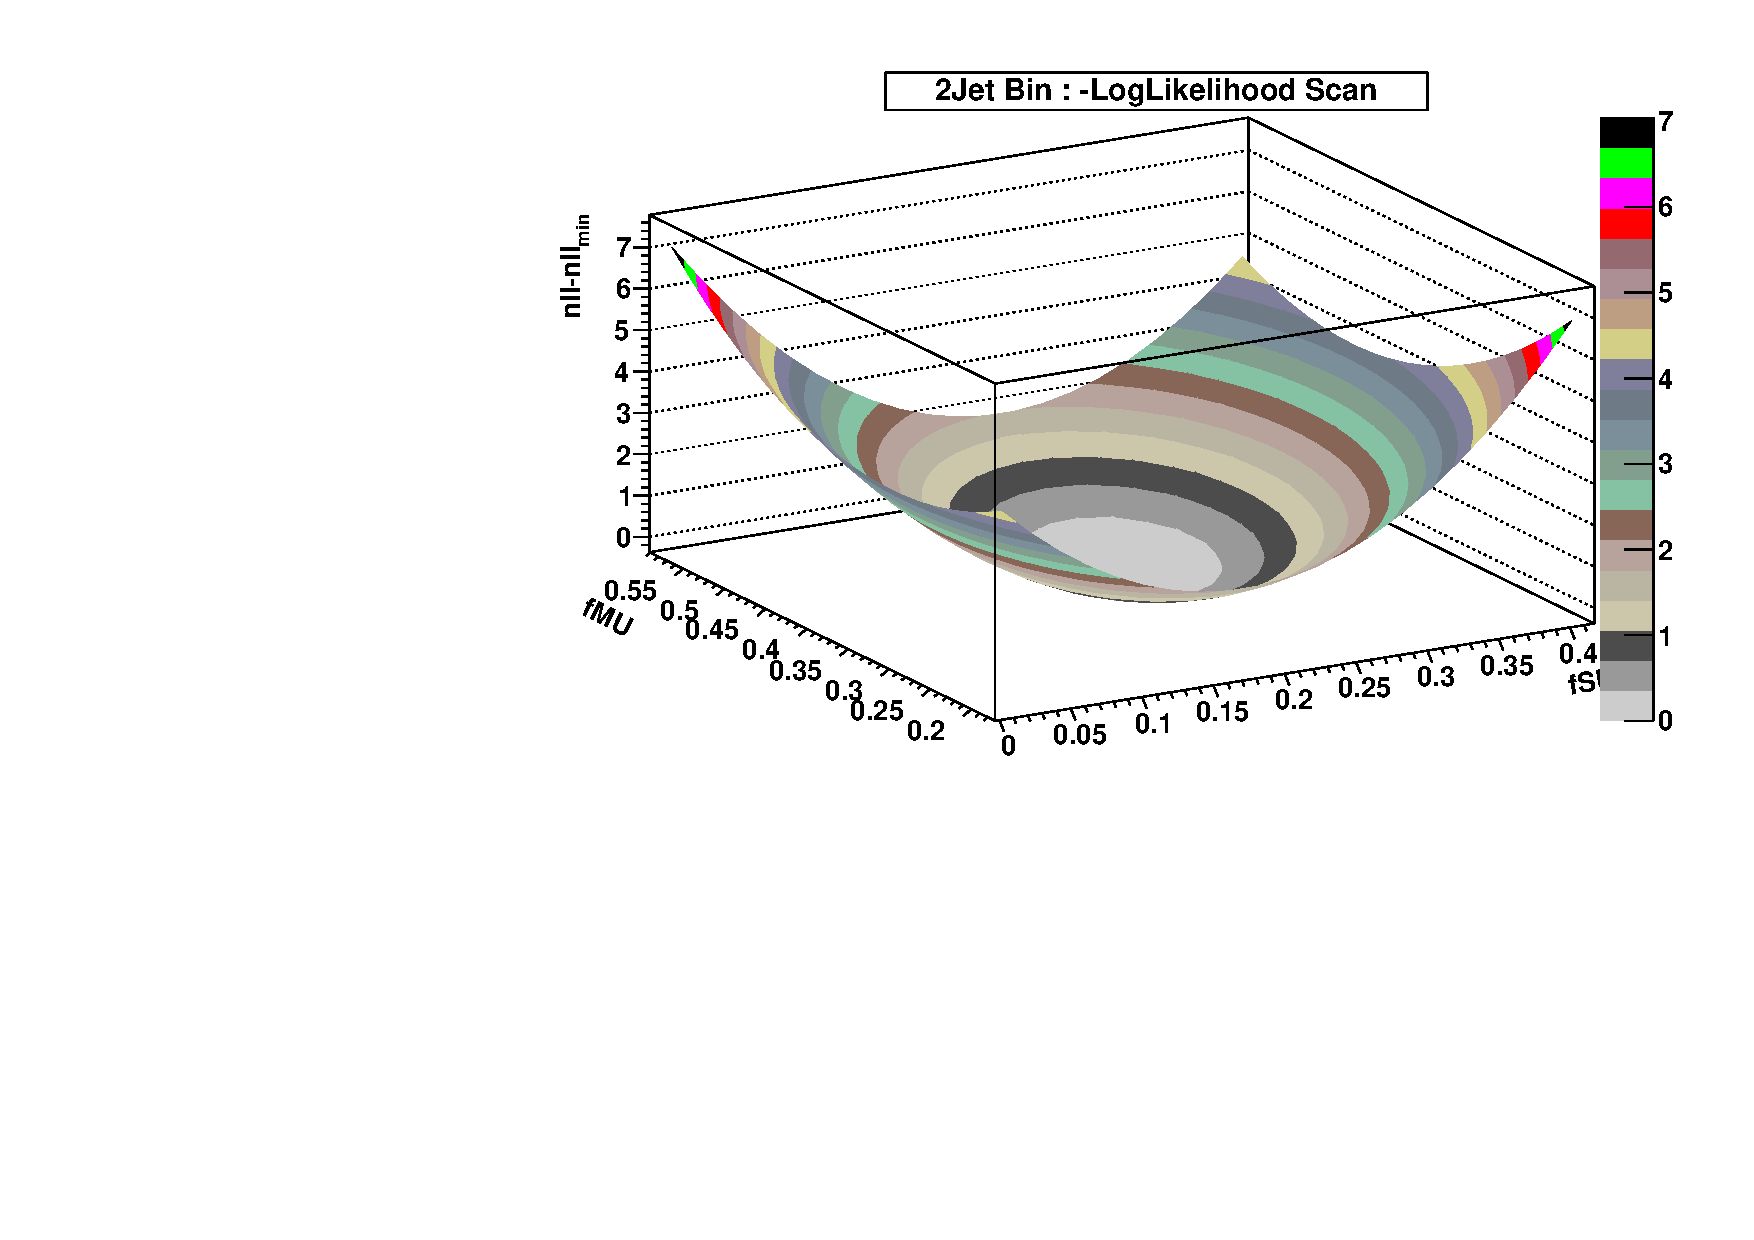
\includegraphics[width=0.49\textwidth]{figs/NLL2DScan_2j_surf.pdf}
%    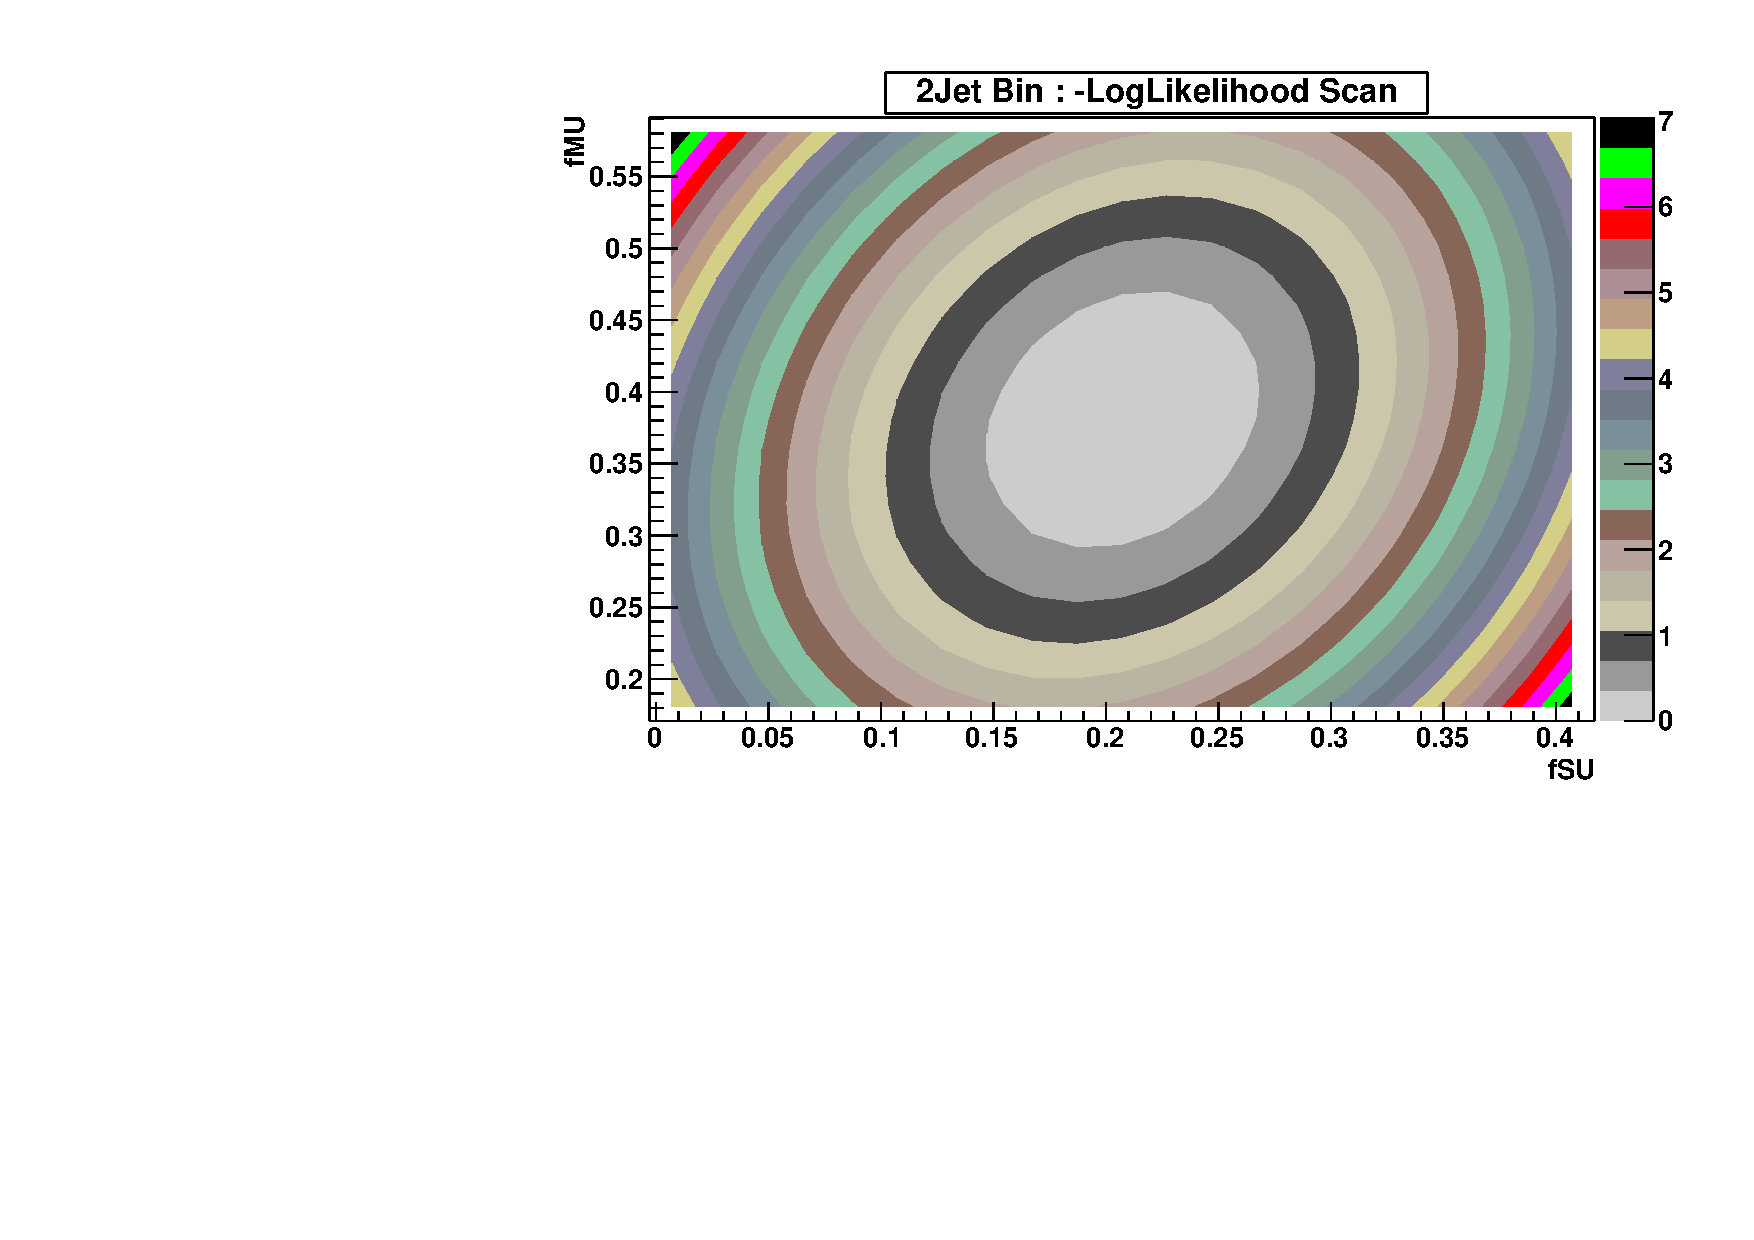
\includegraphics[width=0.49\textwidth]{figs/NLL2DScan_2j_cont.pdf}
%    \caption{Scan over the relative fractions for $q^2$ and matching in the 2-jet bin: Surface (left) and Contour (right).}
%    \label{fig:NLL2DScan_2j}}
%\end{figure}
%%%%%%%%%%%%%%
%\begin{figure}[htb] 
%  {\centering
%    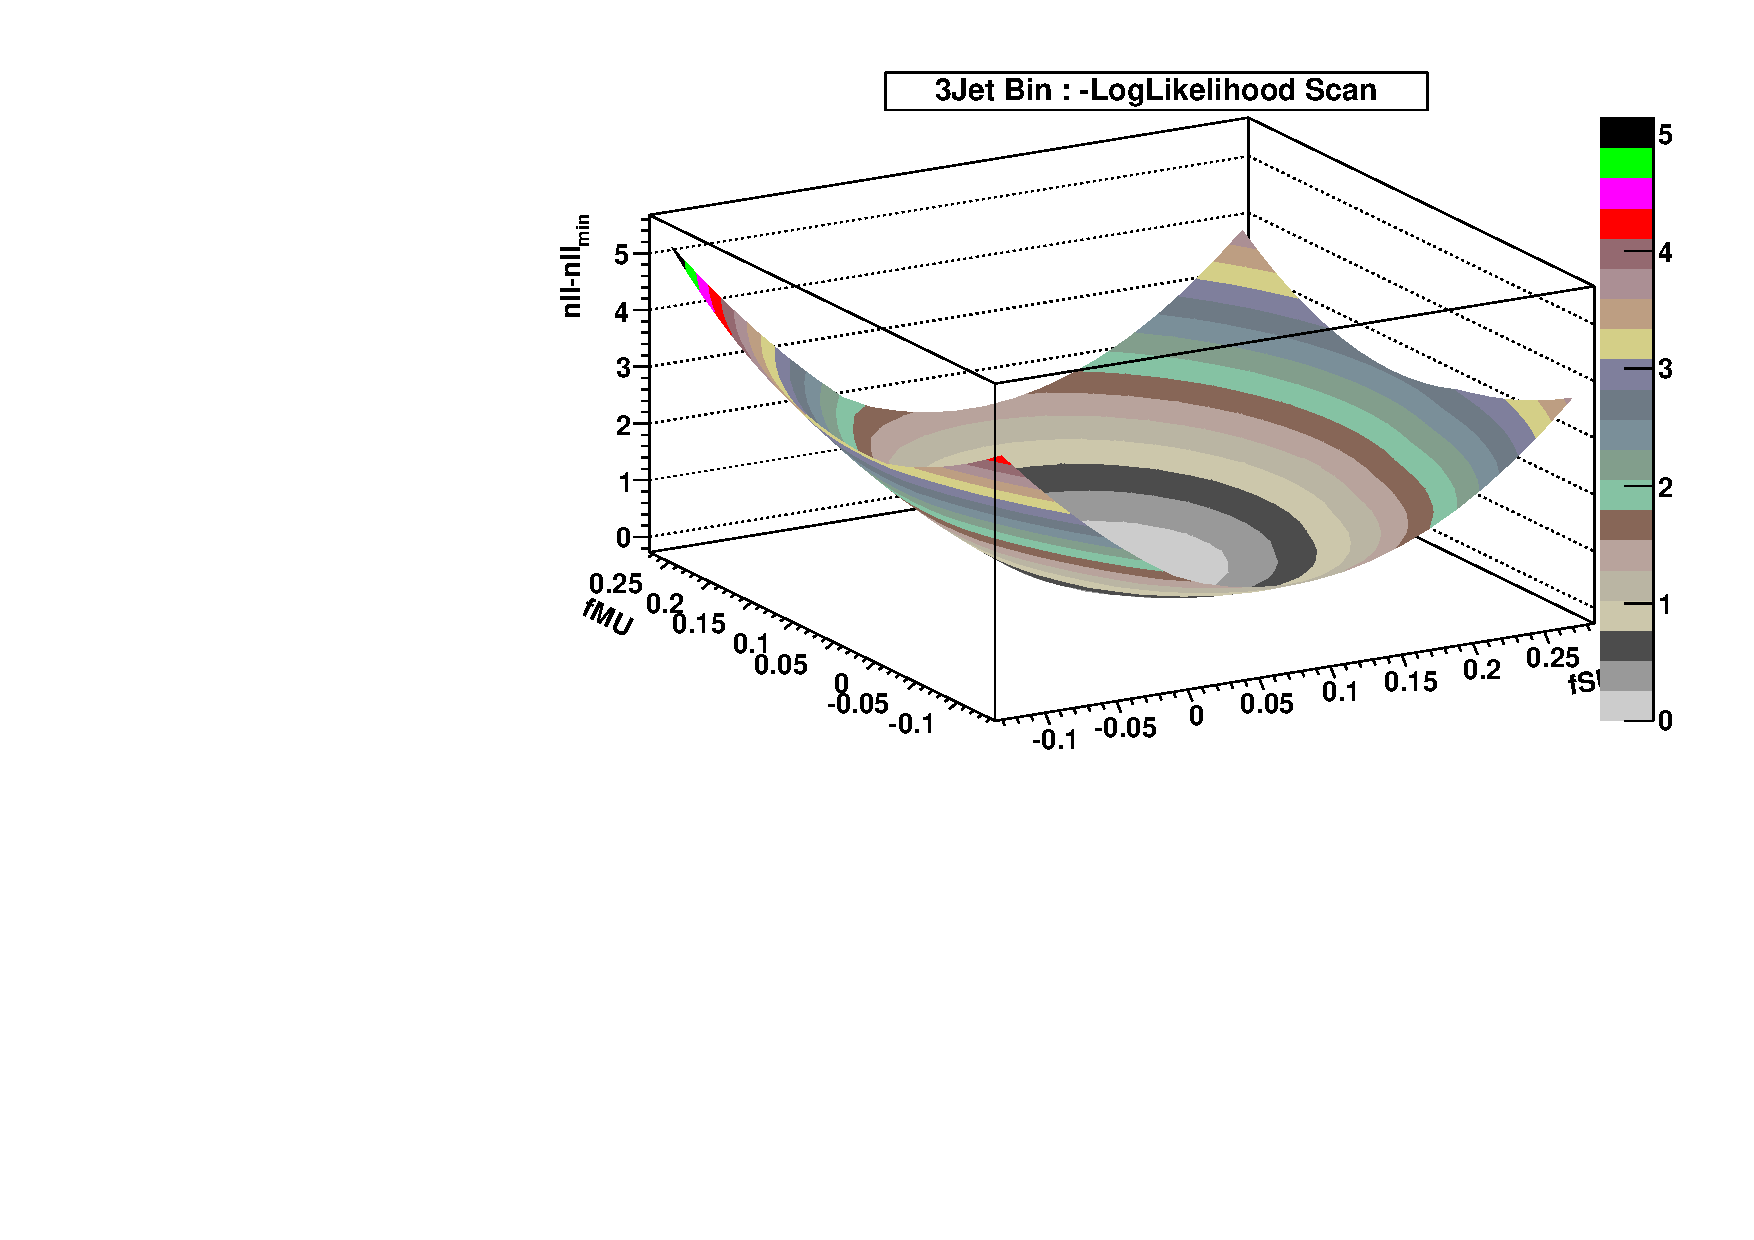
\includegraphics[width=0.49\textwidth]{figs/NLL2DScan_3j_surf.pdf}
%    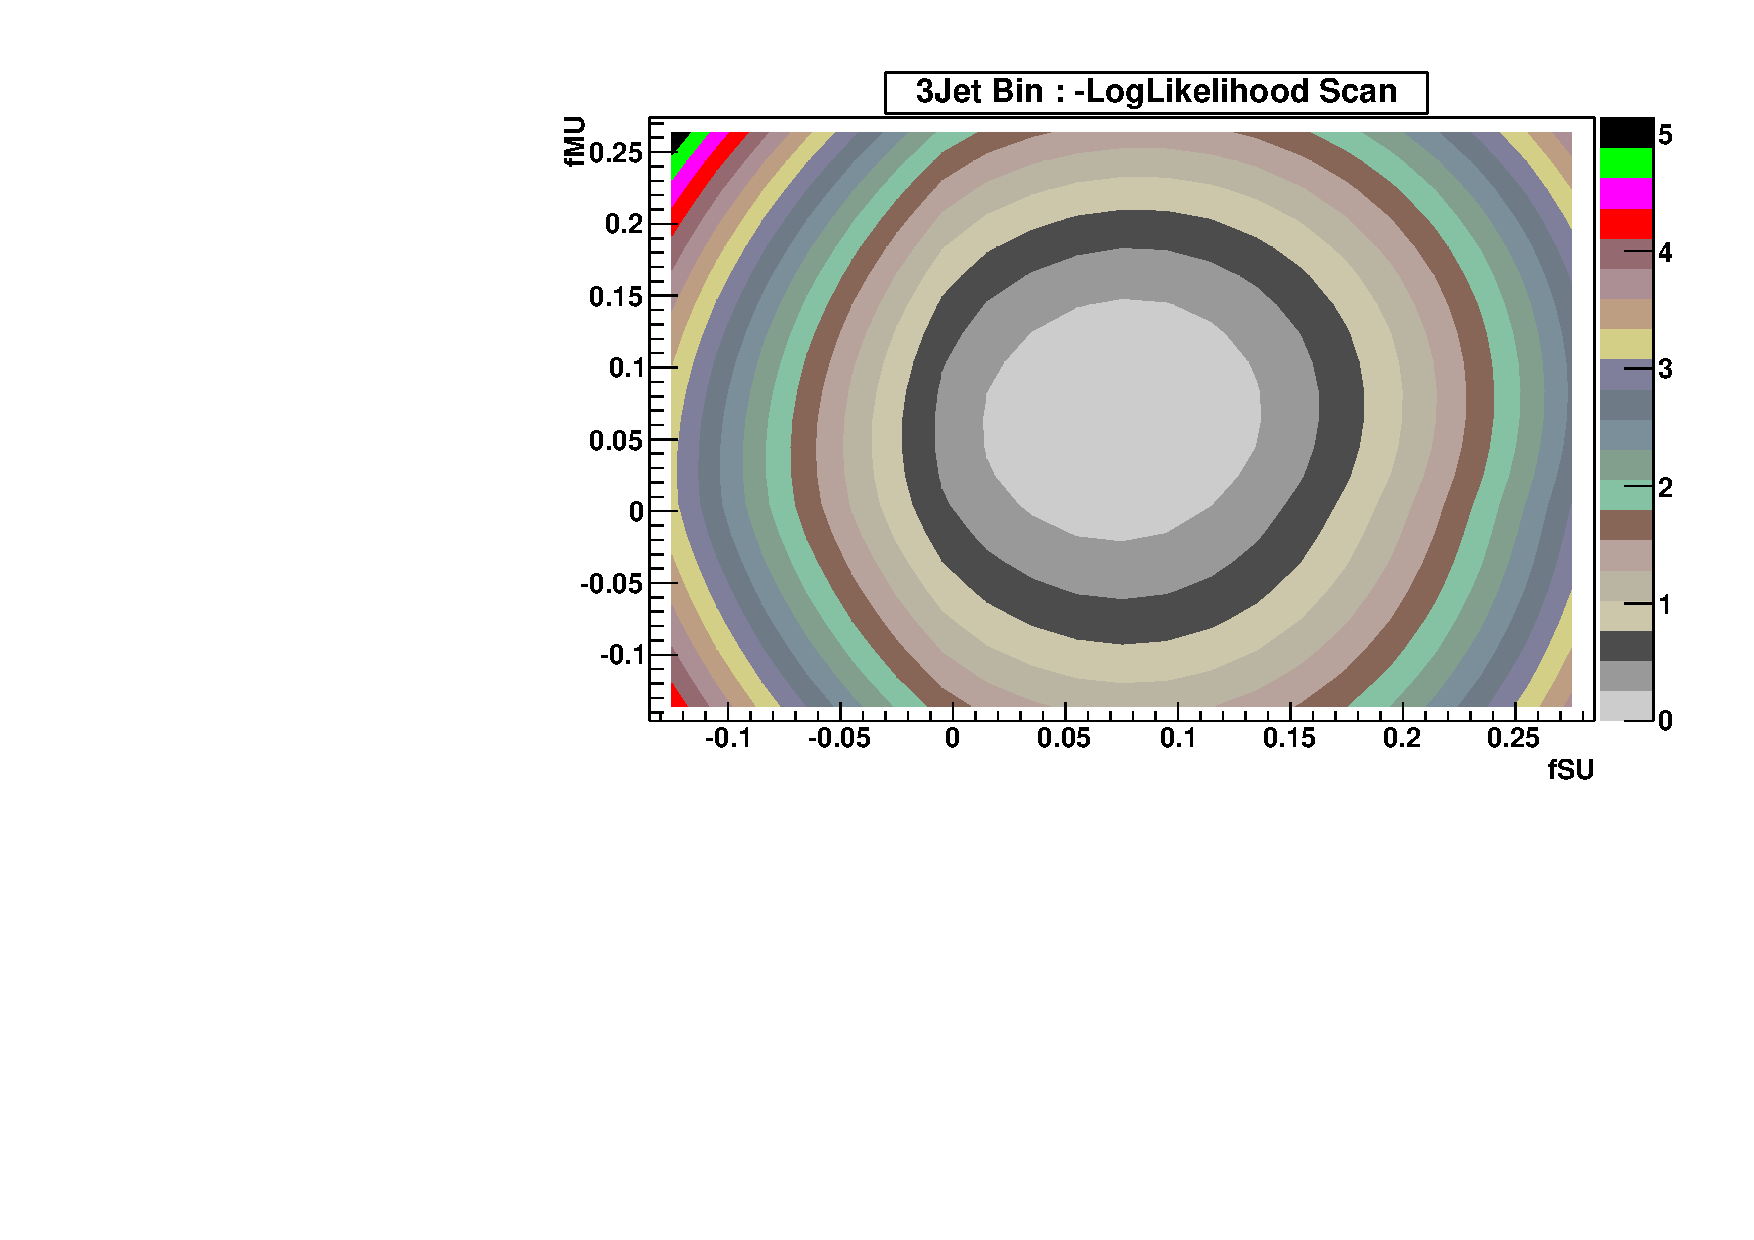
\includegraphics[width=0.49\textwidth]{figs/NLL2DScan_3j_cont.pdf}
%    \caption{Scan over the relative fractions for $q^2$ and matching in the 3-jet bin: Surface (left) and Contour (right).}
%    \label{fig:NLL2DScan_3j}}
%\end{figure}
%%%%%%%%%%%%%%
%%%%%%%%%%%%%%%%%%%%%%%%%%%%%%%%%%%%%%%%
%%%%%%%%%%%%%%%%%%%%%%%%%%%%%%%%%%%%%%%%
\subsection{Jet Energy Scale from the hadronic W in top quark events}
\label{sec:topw}
We reconstruct the hadronic W candidate from an almost pure top data control sample. 
The semileptonic top
events are selected by requiring exactly four jets in the event, out of
which two are b-tagged and the other two are anti-btagged. The
hadronic W candidates are formed from two anti-btagged jets. 
The invariant mass of the hadronic W candidates in the muon,
electron, and combined channels are shown in 
Figs.~\ref{fig:topw:mu},~\ref{fig:topw:el}, and 
\ref{fig:topw:muel}, respectively.  When we propagate the difference in the JES to our
templates they make a negligible difference.
%%%%%%%%%%%%%%%%%%%%%
\begin{figure}[htb] 
  {\centering
    \includegraphics[width=0.75\textwidth]{figs/topwjes/top_overlap_mu.pdf}
    \includegraphics[width=0.49\textwidth]{figs/topwjes/top_data_fit_mu.pdf}
    \includegraphics[width=0.49\textwidth]{figs/topwjes/top_mc_fit_mu.pdf}
    \caption{The invariant mass distribution of the hadronic 
      W candidates in the muon semileptonic top sample. 
      The upper plot shows good agreement between the data and MC. 
      We fit the distribution with a Gaussian and extract the peak
      location for the data (left) and MC (right).}
    \label{fig:topw:mu}}
\end{figure}
%%%%%%%%%%%%%%
\begin{figure}[htb] 
  {\centering
    \includegraphics[width=0.75\textwidth]{figs/topwjes/top_overlap_el.pdf}
    \includegraphics[width=0.49\textwidth]{figs/topwjes/top_data_fit_el.pdf}
    \includegraphics[width=0.49\textwidth]{figs/topwjes/top_mc_fit_el.pdf}
    \caption{The invariant mass distribution of the hadronic 
      W candidates in the electron semileptonic top sample. 
      The upper plot shows good agreement between the data and MC. 
      We fit the distribution with a Gaussian and extract the peak
      location for the data (left) and MC (right).}
    \label{fig:topw:el}}
\end{figure}
%%%%%%%%%%%%%
\begin{figure}[htb] 
  {\centering
    \includegraphics[width=0.75\textwidth]{figs/topwjes/top_overlap_muel.pdf}
    \includegraphics[width=0.49\textwidth]{figs/topwjes/top_data_fit_muel.pdf}
    \includegraphics[width=0.49\textwidth]{figs/topwjes/top_mc_fit_muel.pdf}
    \caption{The invariant mass distribution of the hadronic 
      W candidates in the semileptonic top sample (electron and 
      muon combined). 
      The upper plot shows good agreement between the data and MC. 
      We fit the distribution with a Gaussian and extract the peak
      location for the data (left) and MC (right).}
    \label{fig:topw:muel}}
\end{figure}
%%%%%%%%%%%%%%%%%%%%%%%%%%%%%%%%%%%%%%%%%%%%%%%%%%%%%%%%%%%%%%%%%%%%%%%%%%%
%--------------------------------------------------
\subsection{Lepton selection and trigger efficiency}
\label{sec:LeptonSelectionAndTriggerEfficiency}
%%The lepton trigger and selection is common among several CMS analyses and 
%%we benefit from common studies based on tag-and-probe techniques. 
%%
Systematic uncertainties in the trigger efficiencies in Section~\ref{sec:trigger}
are of the order of 1\%. Systematic uncertainties in the lepton reconstruction
and identification efficiency scale factors are of the order of 2\%. These uncertainties
are accounted for in the final systematics that are input to the limit setter.
%--------------------------------------------------
\subsection{MET uncertainty}
MET directly affects our signal acceptance. 
The uncertainty prescription is discussed in Ref.~\cite{met}.
%https://twiki.cern.ch/twiki/bin/viewauth/CMS/MissingETUncertaintyPrescription
In addition, the MET distribution in the data is $\simeq$3\% wider 
than the MC, and placing a hard MET$>30.0$ cut creates an uncertainty. 
We estimate it by smearing the MET for each event by a Gaussian with 
a $\sigma =0.03*$MET and observing how many events pass the cut. 
Specifically, (Events Passing After Smearing)/(Events Passing Before Smearing) 
=0.998 for both muons and electrons.
%%%%%%%%%%%%%%%%%%%%%%%%%%%%
\subsection{Cross-section of nuisance backgrounds}
The uncertainty in the the cross sections of other backgrounds 
like $\ttbar$,  single top, QCD multi-jets, and Z+jets processes 
is already propagated by letting their normalization (i.e., yield) 
float in the fit within a constraint.
%%%%%%%%%%%%%%%%%%%%%%%%%%%%
\subsection{Luminosity uncertainty}
The latest recommendation for the uncertainty on LHC luminosity is 4.5$\%$~\cite{lumiPAS}.
We propagate this uncertainty to the expected yield of the New Physics 
signal while setting limits.
%%%%%%%%%%%%%%%%%%%%%%%%%%%%

%%%%%%%%%%%%%%%%%%%%%%%%%%%%%%%%%%%%%%%%%%%%%%%%%%%%%%%%%%%%%%%%%%%%%%%%%%
%%%%%%%%%%%%%%%%%%%%%%%%%%%%%%%%%%%%%%%%%%%%%%%%%%%%%%%%%%%%%%%%%%%%%%%%%%
\clearpage{}
\section{Results}
\label{sec:results}
% ---- ---- ---- ---- ---- ---- ---- ---- ---- ---- ---- ---- ---- ---- ----
\par
The well-known formula for the extraction of  a cross section is:
\begin{equation}
\label{eq:xsec}
 \sigma = \frac{N^{\text{Sig}}}
               { A \, \epsilon \, {\cal{L}} }
\end{equation}
where $N^{\text{Sig}}$ is the number of extracted signal events,
$A$ is the signal acceptance corrected for the branching fraction,
$\epsilon$ is the efficiency for all requirements on 
the event selection, and ${\cal{L}}$ is the integrated luminosity.
Using the number of signal diboson events from 
table~\ref{table:FitTotalsAndComparisons} and efficiency $\times$ 
acceptance values from table~\ref{tab:signals}, we obtain the 
WW+WZ cross section values for each disjoint sub-sample as shown in 
table~\ref{tab:measuredCrossSection}
%%%%%%%%%%%%%%%%%%%%%%%%%%%%%
\begin{table}[h]
\begin{center}
  \begin{tabular}{l c}
    \hline  \hline
    Event category &  Measured cross section\\
    \hline
    $\mu jj$        &    $73.41 \pm 15.07$  pb\\
    $ejj$           &    $60.14 \pm 21.50$  pb\\   \hline 
    $\mu jj$,b-tag  &    $76.85 \pm 60.68$  pb\\
    $ejj$,b-tag     &    $22.71 \pm 49.27$  pb\\   \hline 
    Theory prediction~\cite{Campbell:2011bn} &  $65.6 \pm 2.2$ pb\\
    \hline  \hline
  \end{tabular}
\end{center}
\caption{\label{tab:measuredCrossSection}
The measured values of the sum of WW and WZ cross section in each disjoint sub-sample. 
The uncertainties include both statistical and systematic.}
\end{table}
%%%%%%%%%%%%%%%%%%%%%%%%%%%%%

Combining all four channels, we obtain:

WW+WZ cross section = 66.70 $\pm$ 11.74 pb.\\
[Breaking down the uncertainties: 66.70 $\pm$ 8.08 (stat) $\pm$ 8.52 (syst) pb]


We produce combined plots for electrons and muons in
Figs~\ref{fig:combinedNoBtag} and~\ref{fig:combinedWithBtag} for no $b$
tags and with $b$ tags, respectively.

\begin{figure}
\begin{center}
\includegraphics[width=0.45\textwidth]{figs/mjjfit_2jetsample/Diboson_Stacked_combined}
\includegraphics[width=0.45\textwidth]{figs/mjjfit_2jetsample/Diboson_Subtracted_combined}
\includegraphics[width=0.45\textwidth]{figs/mjjfit_2jetsample/Diboson_Pull_combined}
\end{center}
\caption{Combined results of both muons and electrons without btags}
\label{fig:combinedNoBtag}
\end{figure}

\begin{figure}
\begin{center}
\includegraphics[width=0.45\textwidth]{figs/mjjfit_2jetsample/Diboson_btag_Stacked_combined}
\includegraphics[width=0.45\textwidth]{figs/mjjfit_2jetsample/Diboson_btag_Subtracted_combined}
\includegraphics[width=0.45\textwidth]{figs/mjjfit_2jetsample/Diboson_btag_Pull_combined}
\end{center}
\caption{Combined results of both muons and electrons with btags}
\label{fig:combinedWithBtag}
\end{figure}


\subsection{Results including only non b-tag categories}
\label{sec:results2ch}
% ---- ---- ---- ---- ---- ---- ---- ---- ---- ---- ---- ---- ---- ---- ----
Including only non b-tag (both muon and electron) categories, we 
observe 2682 $\pm$ 339 (stat) $\pm$ 357 (syst) WW+WZ events, 
in agreement with the Standard Model expectation. 
This corresponds to a significance of $8.8~\sigma$ 
($7.8~\sigma$ in muon data and $4.4~\sigma$ in electron data) 
when computed using a simple likelihood 
ratio where the nuisance parameters are fixed to their nominal fit 
values in case of the null hypothesis. 
Using the profile likelihood ratio, where the nuisance parameters are 
allowed to vary also for the null hypothesis, the significance 
becomes $4.34~\sigma$ ($4.31~\sigma$ in muon data 
and $1.60~\sigma$ in electron data).


Combining results of muon and electron non b-tag categories, we obtain
the following result for cross section:
$\sigma = 68.89 \pm 8.71 \text{(stat)} \pm 9.70 \text{(syst)}  \pm 1.52 \text{(lumi)}$~pb, 
which is in agreement with the NLO prediction 
$65.6 \pm 2.2$~pb that includes $gg\to\text{WW}$ contribution.

\section{Conclusions}
\label{sec:conclusions}
We have studied the electroweak production 
of two heavy gauge bosons  in events 
with a leptonically decaying W boson and exactly two jets.
The analyzed dataset 
corresponds to an integrated luminosity of 5.0~fb${}^{-1}$ at 
$\sqrt{s} = 7$~TeV collected by the CMS detector at the Large Hadron Collider.
With the kinematic requirements imposed in the analysis, we 
observe 2979 $\pm$ 361 (stat) $\pm$ 402 (syst) WW+WZ events, 
in agreement with the Standard Model expectation. 
The measured value of the sum of WW and WZ cross sections is 
66.7 $\pm$ 8.1 (stat) $\pm$ 8.5 (syst) pb, consistent 
with the standard model prediction of 65.6~pb. 
This is the first observation of diboson events in 
the semi-leptonic final state in a pp collider.
We derive limits on anomalous triple gauge couplings  
using the $p_T$ distribution of the dijet system: 
$ -0.038 < \lambda_Z < 0.030$, 
$ -0.111 < \Delta{\kappa_\gamma} < 0.142$.
These limits are the most stringent at a hadron collider to-date 
and are approaching the sensitivity of combined LEP measurements.


%%%%%%%%%%%%%%%%%%%%%%%%%%%%%%%%%%%%%%%%%%%%%%%%%%%%%%%%%%%%%%%%%%%%%%%%%%
%\newpage
\bibliography{auto_generated}
